\documentclass[12pt]{ruthesis}
\usepackage{latexsym}
%\usepackage{theorem}
%\newtheorem{proposition}{Proposition}

\usepackage{graphicx}	% adds graphics into documents
	\graphicspath{{./figures/}{./figures/ch1/}{./figures/ch2/}{./figures/ch3/}{./figures/ch4/}{./figures/ch5/}{./figures/ch6/}{./figures/apps/}}
\usepackage{grffile}	% allows spaces in figures names
\usepackage{epstopdf}	% converts eps images
\usepackage{bm}			% bold math
\usepackage{amssymb}	% math package
\usepackage{amsmath}	% math package
\usepackage{array}
\usepackage{mathtools}
	\newcolumntype{d}{>{\displaystyle}c}
\usepackage{booktabs}
\usepackage{lscape}
%\usepackage{parskip}	% helps tidy up paragraphs
%	\setlength{\parindent}{35pt}
\usepackage{multirow}	% mutliline cells in tables
\usepackage[usenames,dvipsnames]{xcolor}   % add color to text
%\usepackage[caption=false]{subfig}   	   % Creates subfigures
\usepackage[square,numbers,sort&compress]{natbib}		   % Formats references
\usepackage[colorlinks,citecolor=darkgray,linkcolor=.]{hyperref} % Hyperlinks references
\usepackage[normalem]{ulem} % allows for highlighting, use normalem to protect \emph
\usepackage{enumitem}% Enumerate has too much white space
	\setenumerate[1]{label=\Roman*.}
	\setenumerate[2]{label=\Alph*.}
	\setenumerate[3]{label=\roman*.}
	\setenumerate[4]{label=\alph*.}
\usepackage{outlines} % for displaying outlines
\usepackage{pdfpages} % insert pdf pages from other pdfs

\interfootnotelinepenalty=10000 % make maintaining a single footnote a higher priority, default is 100

% this stuff came with the RU thesis template
\usepackage[toc,page]{appendix}
%\usepackage{cite}
\usepackage{pictex}
\usepackage{fancyhdr}
	\fancypagestyle{frontmatterStyle}{
	\fancyhf{} % clear all header and footer fields
	%\fancyhead[l]{\bfseries \nouppercase \rightmark} % except the center
	\fancyfoot[C]{\thepage} % except the center
	\renewcommand{\headrulewidth}{0pt}
	\renewcommand{\footrulewidth}{0pt}}

%\usepackage{amsmath}
%\usepackage{amssymb}
%\usepackage{graphics}
%\usepackage{epsfig,epsf,rotating}
%\usepackage{subfigure}

%\theoremheaderfont{\itshape} {\theoremstyle{break}
%\newtheorem{Fact}{Fact}[chapter]} \theoremstyle{break}
%\newtheorem{Lem}{Lemma}[chapter] \theoremstyle{break}
%\newtheorem{Thm}{Theorem}[chapter] {\theoremstyle{plain}
%  \theorembodyfont{\rmfamily}  \newtheorem{Prf}{Proof}[chapter]}
%{\theoremstyle{plain}
%  \theorembodyfont{\rmfamily}  \newtheorem{Def}{Definition}[chapter]}

% Custom macros
\let\vec\mathbf % changing \vec from over arrow to bold font

\def\rcurs{{\mbox{$\resizebox{.09in}{.08in}{
\includegraphics[trim= 1em 0 14em 0,clip]{ScriptR}}$}}}
\def\brcurs{{\mbox{$\resizebox{.09in}{.08in}{
\includegraphics[trim= 1em 0 14em 0,clip]{BoldR}}$}}} 

%\newcommand{\hl}{\bgroup\markoverwith
%  {\textcolor{yellow}{\rule[-.5ex]{2pt}{2.5ex}}}\ULon} % creates a highlight command \hl
\newcommand\hl[1]{\colorbox{yellow}{\textcolor{red}{#1}}}
\newcommand{\ket}[1]{\ensuremath{\left| {#1} \right>}} % for Dirac kets
\newcommand{\bra}[1]{\ensuremath{\left< {#1} \right|}} % for Dirac bras
\newcommand{\innerProd}[2]{\ensuremath{\left< {#1} | {#2} \right>}} % for writing the inner product between states
\newcommand{\heaviside}[1]{\ensuremath{\Theta \left( {#1} \right)}} % shortcut for writing the Heaviside function  
\newcommand{\intPot}[2]{\ensuremath{ {#1} + {#2} }} % for writing interatomic potentials
\newcommand{\gs}{\ensuremath{^1S_0}} % saving keystrokes on ground state
\newcommand{\ex}{\ensuremath{^3P_1}} % saving keystrokes on excited state
\newcommand{\Li}[2]{\ensuremath{\text{Li}_{#1}\!\left[ #2 \right]}} %easy polylog
\newcommand{\ssfrac}[2]{\scriptscriptstyle\frac{#1}{#2}\!}
 
\providecommand{\degreeC}{\ensuremath{^\circ}C }  % degree symbol
\providecommand{\e}[1]{\ensuremath{\times 10^{#1}}} % scientific notation
\providecommand{\peakDens}[2]{\ensuremath{n_0 = #1 \times 10^{#2} \, \text{cm}^{-3}}} % shorthand for densities
\providecommand{\abs}[1]{\ensuremath{\lvert {#1} \rvert}} % notation for absolute value

\renewcommand{\inf}{\ensuremath{\infty}} % don't care for \infty, rather \inf for symbol
\renewcommand{\exp}[1]{\ensuremath{\text{exp}\left( {#1} \right)}} % simplify writing exp(x)
  
%%%---%%%---%%%---%%%---%%%---%%%---%%%---%%%---%%%---%%%---%%%---%%%---%%%---%%%---%%%---%%%---%%%---%%%---%%%---
\title{Two-photon photoassociative spectroscopy of ultracold strontium-86}
\ctitle{Two-photon photoassociative spectroscopy of ultracold strontium-86}
\author{James Allen Aman}
\department{Physics and Astronomy}
\school{Rice University}
\degree{Doctor of Philosophy}

\committee {
        Thomas C. Killian, Chair \\
        Professor of Physics and Astronomy \and
        Randall G. Hulet \\
        Fayez Sarofim Professor of Physics and Astronomy \and
        Kevin F. Kelly\\
        Associate Professor of Electrical and Computer Engineering
}

\address{Houston, Texas}
\donemonth{July} \doneyear{2019} 

\makeindex

\begin{document}
  \begin{frontmatter}
  \pagestyle{frontmatterStyle}
   \pagenumbering{roman}
   \maketitle
   
   \phantomsection
   \begin{abstract}

"Lorem ipsum dolor sit amet, consectetur adipiscing elit, sed do eiusmod tempor incididunt ut labore et dolore magna aliqua. Ut enim ad minim veniam, quis nostrud exercitation ullamco laboris nisi ut aliquip ex ea commodo consequat. Duis aute irure dolor in reprehenderit in voluptate velit esse cillum dolore eu fugiat nulla pariatur. Excepteur sint occaecat cupidatat non proident, sunt in culpa qui officia deserunt mollit anim id est laborum."

\end{abstract}



   
   \phantomsection
   \begin{acknowledge}

It is difficult to over state how much I have learned during my time in grad school. Not only pertaining to physics, engineering, and computer science but also about myself, my friends, and my communities.

I owe so much to Brian DeSalvo for being an inspiration. It was Brian who showed me my first Bose-Einstein condensate 

I bugged him relentlessly as a naive undergraduate with so many questions.



\end{acknowledge}
   
   \tableofcontents
   \listoffigures
   \listoftables
  \end{frontmatter}
  
\pagenumbering{arabic}
\linespacing{1.7}

%Main chapters
\chapter{Introduction}
\label{ch:intro}

The ability to engineer and manipulate quantum states lies at the heart of modern atomic physics experiments using ultracold gases \cite{Davis1995,Anderson1995,Bradley1995,DeMarco1999,Lang2008,Ni2008}. Two important tools for this pursuit are Feshbach resonances \cite{Chin2010,Kohler2006} and optical lattices \cite{Bloch2008}. This proposal will detail our recent work building and characterizing a three-dimension optical lattice for use with ultracold and quantum degenerate gases of neutral strontium. Furthermore, we will present the first experiment we hope to pursue with the optical lattice; the creation of Feshbach molecules using an optical Feshbach resonance. We will also briefly discuss other future plans such as the production of highly excited ground state Sr$_2$ dimers through adiabatic internal state transfer.

Should probably mention somewhere that this is long-range PA, in contrast to short-range stuff being explored now.

Julienne form of the corss section 6.16 in CM. Discuss how important the phase space density is, the timescale for interactions, and the complex 

\cite{Aman2018}

\section{Few-body physics}
\label{sec:few-body}

field of photoassociation in ultracold gases, wherein studies of molecular structure have revealed the most accurate descriptions of atomic interactions and have become a fundamental probe of the ultracold toolbox \cite{Jones2006}.

\section{Halo molecules}
\label{sec:halo}

Mostly studied in helium

Comes from bound state of the dirac potential. Unsure how much detail I want right here

Check out CM Juleinne pg 229. He has a ref

\section{Properties of strontium}
\label{sec:sr}

	\begin{figure}
		\centerline{
		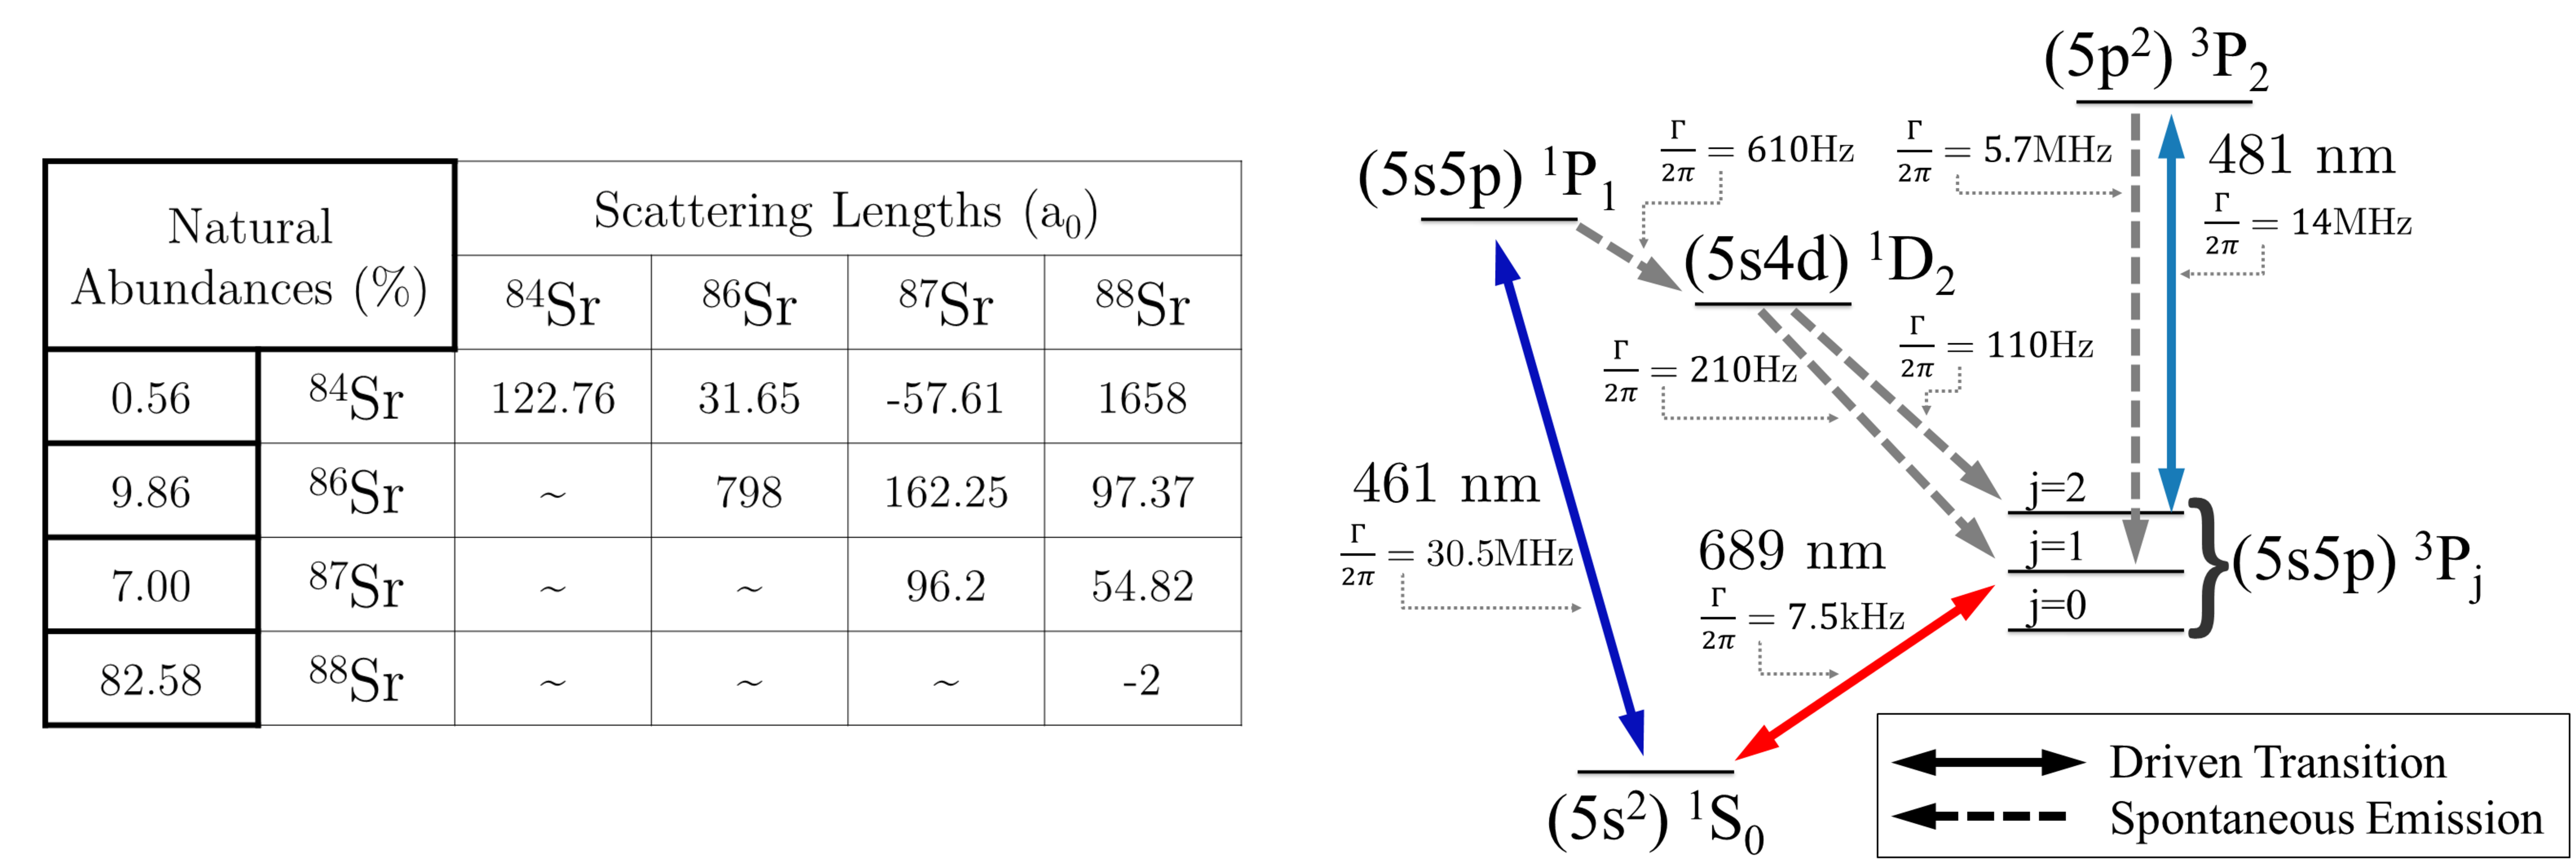
\includegraphics[height=0.25\textheight]{Fig1_strontium_properties.pdf}}
		\caption{Properties of strontium. Left: Natural abundances and s-wave scattering lengths for all mixtures of Sr. Right: Simplified energy level diagram of Sr showing the relevant states used for trapping and cooling of the atomic gas}
		\label{fig:energy_level_diagram}
	\end{figure} 
The experiments in this proposal will be realized using an ultracold gas of atomic strontium. Fig.\;\ref{fig:energy_level_diagram} shows all of the stable isotopes of strontium, their natural abundance, as well as their inter-particle scattering lengths. The isotopic differences in strontium have important implications for their use in certain experiments. For example, none of the bosonic isotopes of strontium ($^{88}$Sr, $^{86}$Sr, or $^{84}$Sr) display hyperfine structure since they have no nuclear spin, $\vec{I}=0$. However, the fermionic isotope $^{87}$Sr has a large nuclear spin, $\vec{I}=9/2$, which makes it an ideal candidate for exploring exotic phases of quantum magnetism \cite{Beverland2016,Cazalilla2014,Chen2015}. In the studies presented in this proposal, we are sensitive to the isotopic shifts of the bosonic photoassociation lines along the $^1S_0\!\rightarrow\!^3P_1$ transition as well as the various interspecies scattering lengths.

\begin{figure}
\label{fig:energy_level_diagram}
	\centerline{
	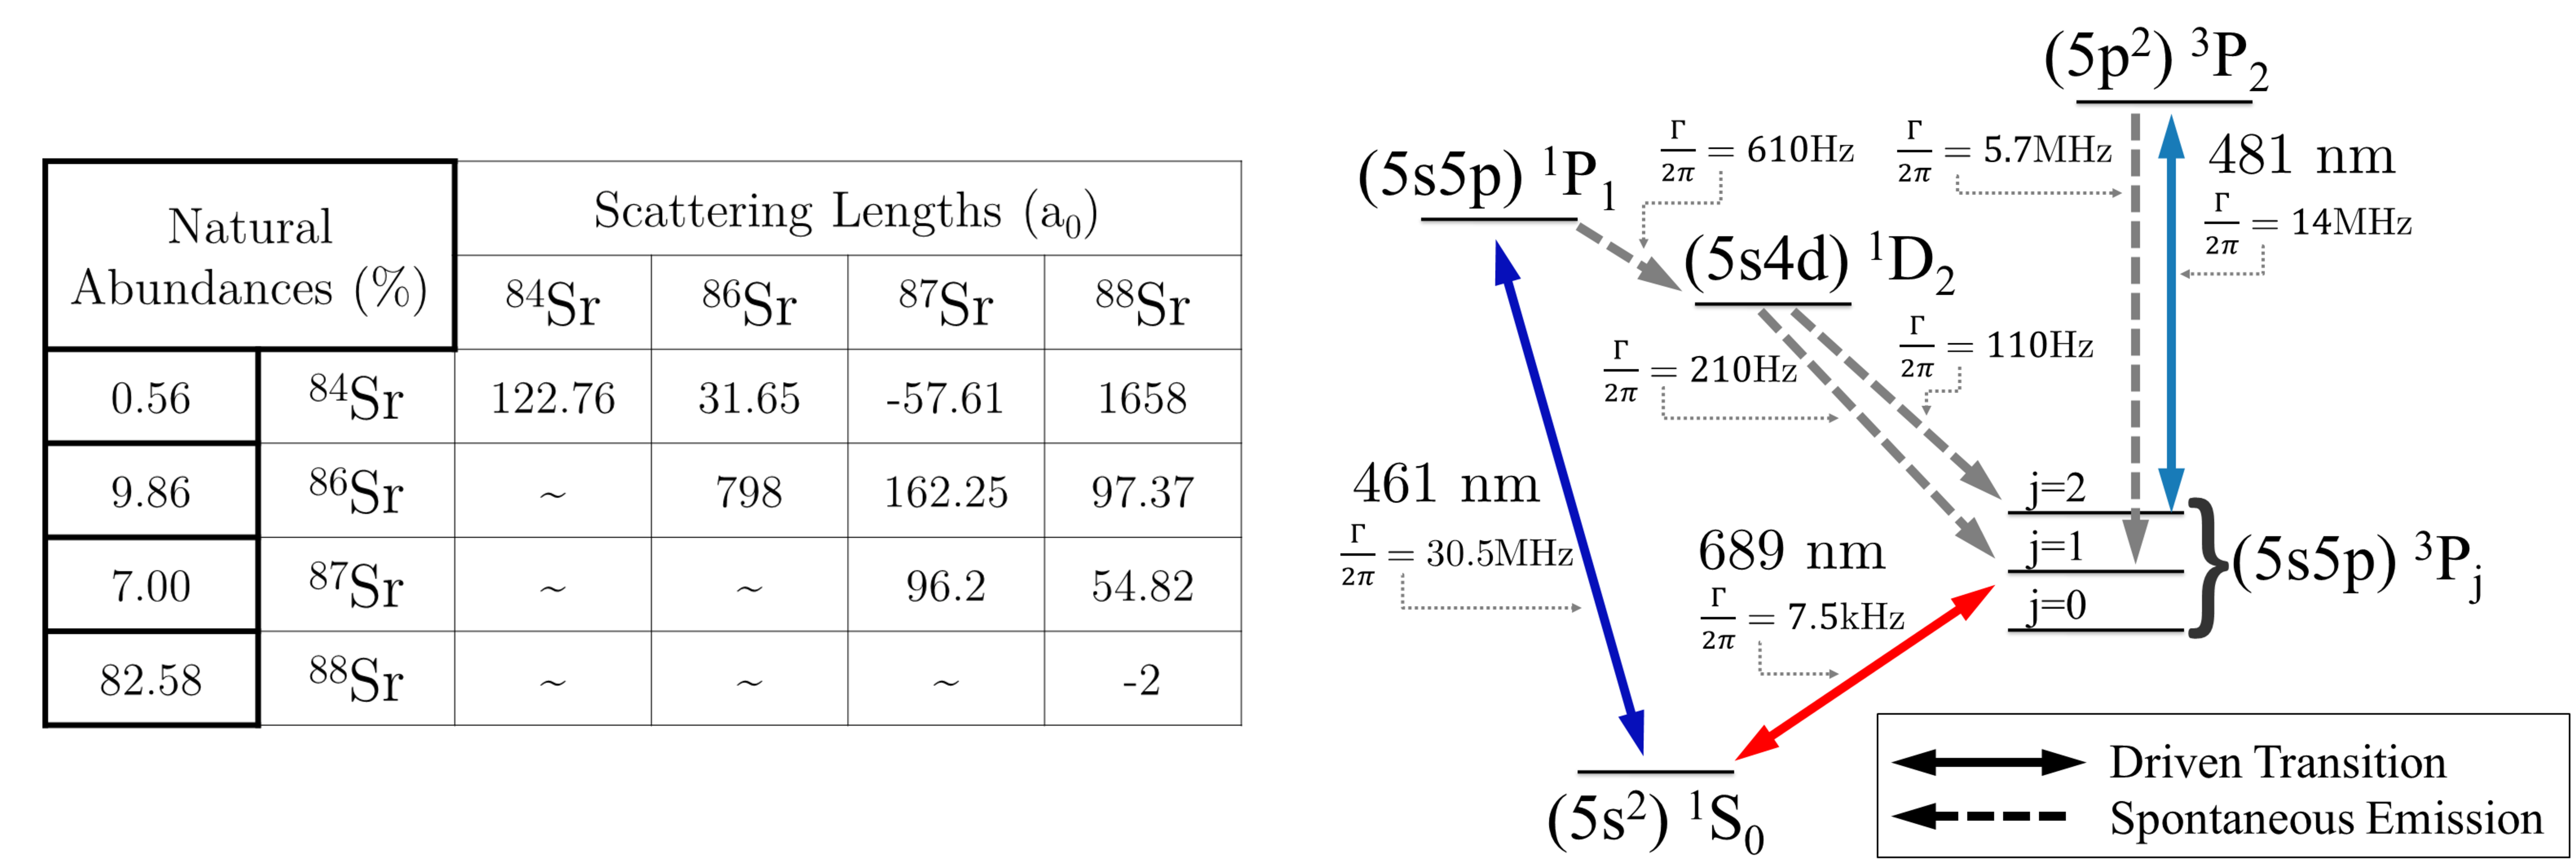
\includegraphics[height=0.25\textheight]{strontium_properties.pdf}}
	\caption{Properties of strontium}{Properties of strontium. Left: Natural abundances and s-wave scattering lengths for all mixtures of Sr. Right: Simplified energy level diagram of Sr showing the relevant states used for trapping and cooling of the atomic gas}
\end{figure} 

\section{Thesis Outline}
\label{sec:outline}

"Lorem ipsum dolor sit amet, consectetur adipiscing elit, sed do eiusmod tempor incididunt ut labore et dolore magna aliqua. Ut enim ad minim veniam, quis nostrud exercitation ullamco laboris nisi ut aliquip ex ea commodo consequat. Duis aute irure dolor in reprehenderit in voluptate velit esse cillum dolore eu fugiat nulla pariatur. Excepteur sint occaecat cupidatat non proident, sunt in culpa qui officia deserunt mollit anim id est laborum."


\begin{equation} 
\label{eq:1dlattice}
		 V(x) = V_{lat} \; \sin^2(k_L x)
\end{equation}




\chapter{The Neutral apparatus}
\label{ch:chap2}

The Neutral apparatus has been one of the pioneering experiments for the trapping, cooling, and creation of quantum degenerate gases of neutral strontium \hl{BEC refs}. 
As such, there is a plethora of previous theses and publications which extensively outline the details for how to achieve these goals. \hl{refs}. 
In particular, we refer the reader to the PhD theses of previous Killian lab students: Francisco Camargo, Brian DeSalvo, Mi Yan, Pascal Mickelson, Natali Martinez de Escobar, and Sarah Nagel. 
Additionally, the PhD work of Simon Stellmer \cite{SimonStellmer2013} and review of strontium quantum degenerate gases are also highly recommended reading \cite{StellmerRev2013}.

Building upon this previous work, this chapter will forego an extensive review of the basic laser cooling techniques for strontium. 
We refer the reading to the works listed above for a formal discussion of the theory behind laser cooling and trapping.
Instead, we will focus on the systems and processes which are crucial to the operation of the experiment with an emphasis on technical findings and changes which remain, as of yet, mostly undocumented.

Furthermore, it has been nearly a decade since the last broad apparatus overview \cite{MartinezdeEscolar2010} and the experiment has grown significantly in complexity in the intervening years.
Therefore, the goal of this chapter is to serve as a reference for future work and students. 
In this spirit, this chapter will be highly technical and provide an in-depth review of the operation and current status of the Neutral apparatus.
Where appropriate we will refer the reader to the relevant original thesis or published work.

This chapter will begin with a brief overview of our trapping procedure in order to contextualize the remaining sections focusing on the hardware including the vacuum system, various laser systems, and RF and electronics.
Furthermore, we will conclude with an outline of recent software implementations used to interface the digital world to the physical.
Detailed guides for this software can also be found in App. \ref{app:neuKLEIN}.

\section{Experimental procedure} \label{sec:trapping}
\setcounter{footnote}{0}
% Intro
Our experiments begin by cooling and trapping atomic strontium utilizing well-established atomic physics techniques \cite{Metcalf1999,Katori1999,Ido2000,Nagel2003,Mukaiyama2003a,Loftus2004,mmy09a,sth09a,Mickelson2010ja,Tey2010a,dym10a,stg10}. 
Fig.\,\ref{fig:energyLevels} shows the simplified energy level diagram employed in our cooling process. 
Once cooled, we typically obtain bulk samples in an optical dipole trap containing on the order of $10^6$ atoms at temperatures $<1\mu$K and densities between $10^{12} - 10^{15}\,$cm$^{-3}$ depending upon the isotope. 

The procedure outlined below is generally followed for trapping all isotopes of strontium with the major difference being timescales and laser frequencies.
Trapping of the bosonic isotopes of strontium is nearly identical across isotopes while fermionic $^{87}$Sr presents a greater challenge due to its high nuclear spin, $I=9/2$.
In short, due to the change in spin between the singlet and triplet series, there is a mismatch in the Zeeman shifts of the $^1S_0$ and $^3P_1$ states which leads to a change in sign of the Zeeman shift across the magnetic sublevels of the $^3P_1\,(F=11/2)$ hyperfine state of 87.
This sign change results in anti-trapped states causing atoms to be expelled from the MOT laser acting on the $^1S_0\,(F=9/2)\,\rightarrow\,^3P_1\,(F=11/2)$ transition.
The solution is then to add an additional laser addressing the $^1S_0\,(F=9/2)\,\rightarrow\,^3P_1\,(F=9/2)$ transition to randomize the $m_F$ populations in the $^1S_0$ ground state.
For a more thorough and detailed discussion of the relevant physics of trapping $^{87}$Sr in the red MOT, we refer the interested reader to the fermion portion of section 2.7.3 in the PhD thesis of Simon Stellmer \cite{SimonStellmer2013} and section 2.2.1 of Pascal Mikelson's PhD thesis \cite{Mickelson2010b}.

\noindent \rule{75pt}{0.5pt} \newline
The trapping process begins with vaporizing metallic strontium loaded in an oven heated to approximately 400 $^{\circ}$C. 
This strontium vapor escapes through thin collimating tubes to produce a partially collimated beam with a mean velocity of $\sim450$ m/s.
To aid in collimation, the atoms undergo a stage of transverse two dimensional optical molasses which is elongated and retro-reflected.
This helps increase the atom flux into the Zeeman slowing stage and we typically observe an approx. 7x improvement in trapped atom number with the 2D collimator versus without.
The majority of cooling is done using 461\,nm light acting on the strongest dipole allowed transition between the $^1S_0\,\rightarrow\,^1P_1$ states.
The excited state lifetime of 5 ns ($\Gamma=30.5$MHz) and large energy separation between the states results in a hefty saturation intensity of 40.5 mW/cm$^2$ for this transition.
Therefore laser power on order of 100 mW are necessary to produce large optical forces and rapid cooling rates.

Once atoms have entered the magnetic field of the Zeeman slower, the highest velocity atoms begin to scatter photons from the Zeeman beam red detuned by approx. 16x the natural linewidth.
Large detunings help to eliminate unwanted photon scattering from the Zeeman beam once atoms have been sufficiently cooled and are accumulating in the MOT fields of the science chamber\footnote{
We note that while the principle functioning of the Zeeman slower only relies on the magnitude of the B-field along the solenoid, there is an interaction to be considered between the anti-Helmholtz MOT field and the decaying fringe fields of the Zeeman slower which can either lead to the fields adding or subtracting near the interface of the Zeeman and science chamber.
This subtle detail can have a large impact on trapping efficiency as we determined around 2014 when the current direction of the Neutral Zeeman slower was reversed from clockwise to anti-clockwise and we observed a 2x increase in trapped atom number at the conclusion of the blue MOT stage.}.

Once atoms have been slowed down to approx. 30 m/s we can capture using a magneto-optical trap (MOT) also working on the $^1S_0\,\rightarrow\,^3P_1$ transition. 
The optimal trapping frequency is tweaked for each isotope using our tunable sat. abs described in Sec. \hl{give ref}.
However, the typical detuning is approx $-3\Gamma/2 \approx -45$ MHz. 

MOT operation using this transition comes with the significant drawback that the Doppler temperature is relatively high at $T_D\approx1$ mK. 
The $J=0$ ground state of strontium also precludes the use of standard Sisyphus cooling techniques as there is only a single $m_J$ state available for bosonic strontium and far too many $m_F$ states in fermionic strontium.
Additionally, the $^1S_0\,\rightarrow\,^3P_1$ transition is not completely closed as shown in \;\ref{fig:energyLevels} resulting in population of the long-lived $^3P_2$ state. 
Fortunately, both of these obstacles are easily overcome.

The leak to the $^3P_2$ state results in population of magnetically trappable low-field seeking $m_j$ states. 
These atoms are trapped by the anti-Helmholtz field of the MOT and are dark to the 461\,nm light \hl{natali refs (I think) [78, 79, 80, 65]}.
This allows us to take advantage of the long lifetime of the metastable $^3P_2$ state and accumulate a large number of atoms which can then be repumped back down to the $^1S_0$ ground state.
One drawback to this process is the long timescale required for a significant number of atoms to accumulate in the magnetic trap compared to the MOT.
However, the lifetime of the magnetic trap is typically limited by background pressure (approx. 15 - 25s) and therefore the maximum number of atoms which can be held by the magnetic trap is much greater than in the MOT.
On average, an atom will fall into the $^3P_2$ state after scattering $10^5$ photons from the $^1S_0\,\rightarrow\,^3P_1$ transition and even then, only 2 out of 5 of the magnetic sub-levels are trappable.
Repumping is achieved via a 481\,nm transition along the $(5s5p)\,^3P_2\,\rightarrow\,(5p^2)\,^3P2$ transition for approx. 50ms.
During the repumping exposure we continue to illuminate the cloud with 461\,nm light but reduce the light intensity by an order of magnitude.
We refer to this stage as the "cold" blue MOT and find that reduction of the intensity, while maintaining consistent laser detuning, increases the transfer efficiency into the red MOT stage.
\footnote{We have explored ramping the laser intensity closer to atomic resonance as we expected reduced intensity at farther red-detuning to result in a weakened trapping force.
However, we did not find any improvement with the added complexity of varying the blue laser frequency during this stage.}

Once the atoms have been returned to the ground state, we begin a second MOT stage using the narrow intercombination transition $^1S_0\,\rightarrow\,^3P_1$ to cool below 1 mK.
\hl{would like to address the saturation intensity and say how the time scale between scattering can become important}
The $(5s5p)\,^3P_1$ state has a reasonably long lifetime of 21 $\mu$s ($\Gamma/2\pi=7.5$ kHz).
This long lifetime and near-IR wavelength transition has a Doppler limit of approx. \hl{450 nK??} and a recoil temperature of \hl{900 nK??}.
The narrow line MOT operates in a different regime compared to typical dipole allowed MOTs as the narrow linewidth means that only a thin shell of the atomic cloud is resonant at a given laser detuning and magnetic field value.
We can simulate the behavior of a broad transition by frequency modulating the 689\,nm light using voltage controlled RF sources coupled to the light via an acouto-optic modulator (AOM). 
Additionally, we begin the narrow line cooling with the center frequency, amplitude of modulation, and laser intensity at large values in order to trap the initially hotter atoms from the blue MOT stage. 
As cooling with the 689\,nm light becomes effective, we dynamically vary these three parameters along with the magnetic field gradient in order to cool the entire sample.
Ultimately, the MOT is reduced to single frequency operation at low laser intensity to and we achieve final temperatures between 1 - 2 $\mu$K after 400 ms of cooling.

During the last 50 - 100 ms of the 689 MOT (typically during single frequency operation) we additionally overlap the high intensity 1064\,nm optical dipole trap (ODT).
The red MOT can then cool atoms into the typically 10 $\mu$K deep ODT with relative ease with transfer efficiencies as high as 75\%. 
Next, we extinguish the red MOT and allow a period of free evaporation for the sample to equilibrate in the ODT before beginning forced evaporative cooling to produce our final sample of ultracold or quantum degenerate gas.

The end of the evaporation typically marks the beginning of the experimental phase and the divergence of our protocol into the specific procedures necessary. 
These may include ramping or pulsing on lattice beams, exciting a collective mode, probing the gas with PAS laser, shelving, etc. 
Once we have completed the experimental phase, we measure the cloud characteristics via absorption imaging along the $^1S_0\,\rightarrow\,^1P_1$ transition. 
Typically we perform absorption imaging following a time-of-flight so as to measure both the atom number and temperature at the time of release. 
However, this is not strictly necessary and certain experiments may result in low atomic densities which are not amenable to a time-of-flight due to their low optical depth.

\subsection{Characteristic performance} \label{sec:benchmark_trapping}
The following tables outline typical trapping performance at various stages of the cooling precedure for each isotope. Note, that while we have demonstrated the ability to dual trap 84 and 87, full characterization and optimization of this process is currently the subject of investigation.




%Remember the switch to single frequency
%What about values for the experiments?
%\paragraph{Daily statistics} \label{sec:dailyStats}
%The following is a table of daily measurements used for monitoring the long-term performance of various laboratory systems..
%We have found these parameters to be most the most informative and therefore should be recorded on days the apparatus will performing trapping.
%Some columns do not contain data as the requisite measurements have evolved over the years\footnote{The full spreadsheet is currently located at \texttt{KillianDrobo:\textbackslash\textbackslash Neutral\textbackslash Daily Statistics.xlsx}}.

\pagebreak
\section{Vacuum system and atom source} \label{sec:vac}
\setcounter{footnote}{0}
\paragraph{Overview}
	
The Neutral apparatus is built around a custom stainless steel chamber positioned above the table to facilitate optical access. Typical pressures are in the ultrahigh vacuum regime, $<1\times10^{-10}$ torr. 
Details on the original construction can be found in Natali (App. A.10) and Pascal's theses \cite{MartinezdeEscolar2010,Mickelson2010b}. The master's of Francisco Camargo \cite{Camargo2015} outlines the construction of the similar Rydberg apparatus. This more recent apparatus has benefited from the many lessons learned during the early life of the Neutral experiment.
\newline

% Complete assembly
\noindent Figure \ref{fig:vacuumSystem} shows a complete overview of these assemblies which form our vacuum system.
	\begin{figure} 
		\centerline{
		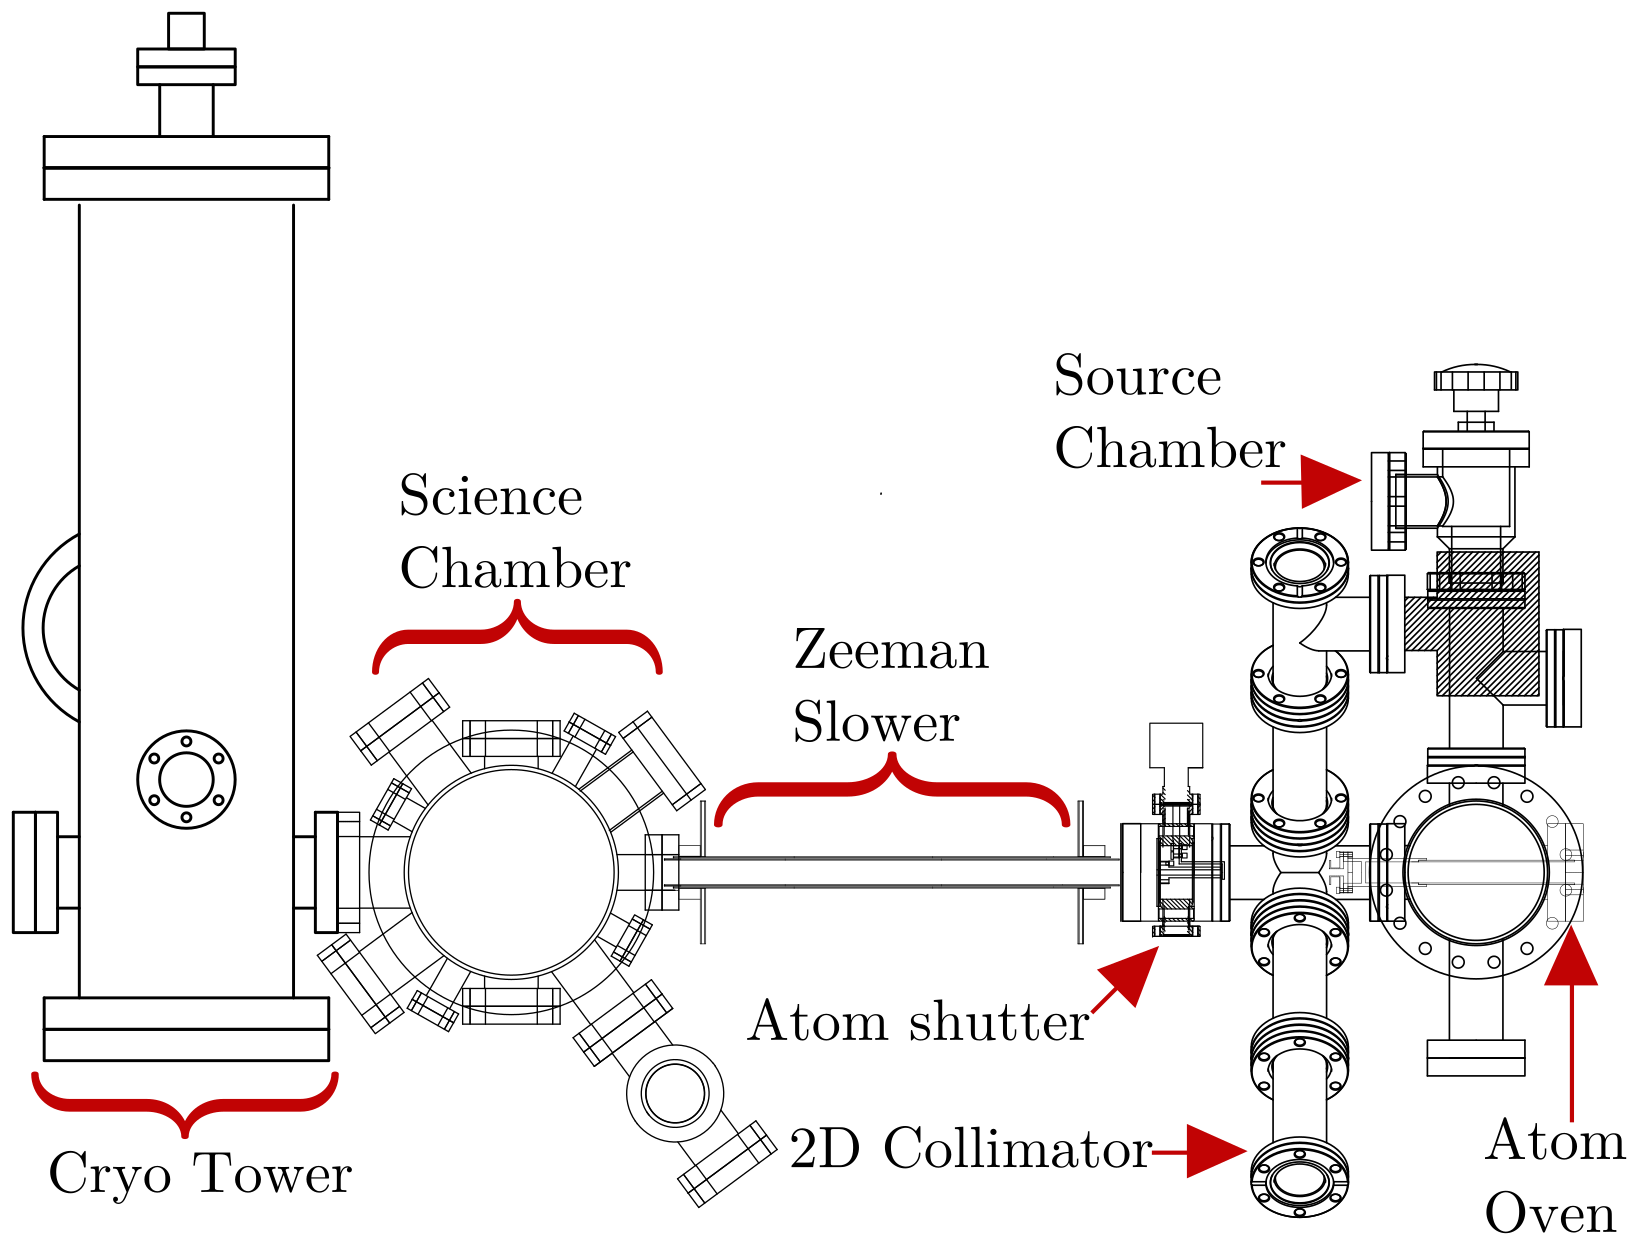
\includegraphics[width=\textwidth]{Vaccum_overview.png}}
		\caption{Neutral apparatus vacuum system}{Some components are rotated to provide easier identification. Not shown are the bellows which extend from the upper angle valve of the source chamber to the metal valve shown in Fig.\,\ref{fig:cryoTower}.}
		\label{fig:vacuumSystem}
	\end{figure}		
Figures \ref{fig:sourceSideView} - \ref{fig:cryoTower} also show various views of the atom source, 2D collimator, and cryo tower assemblies. Note the red markers and green arrows denote the positions of heater bands and thermo-couples respectively. For more information please see App. \ref{app:breakingVacuum}.
	\begin{figure} 
		\centerline{
		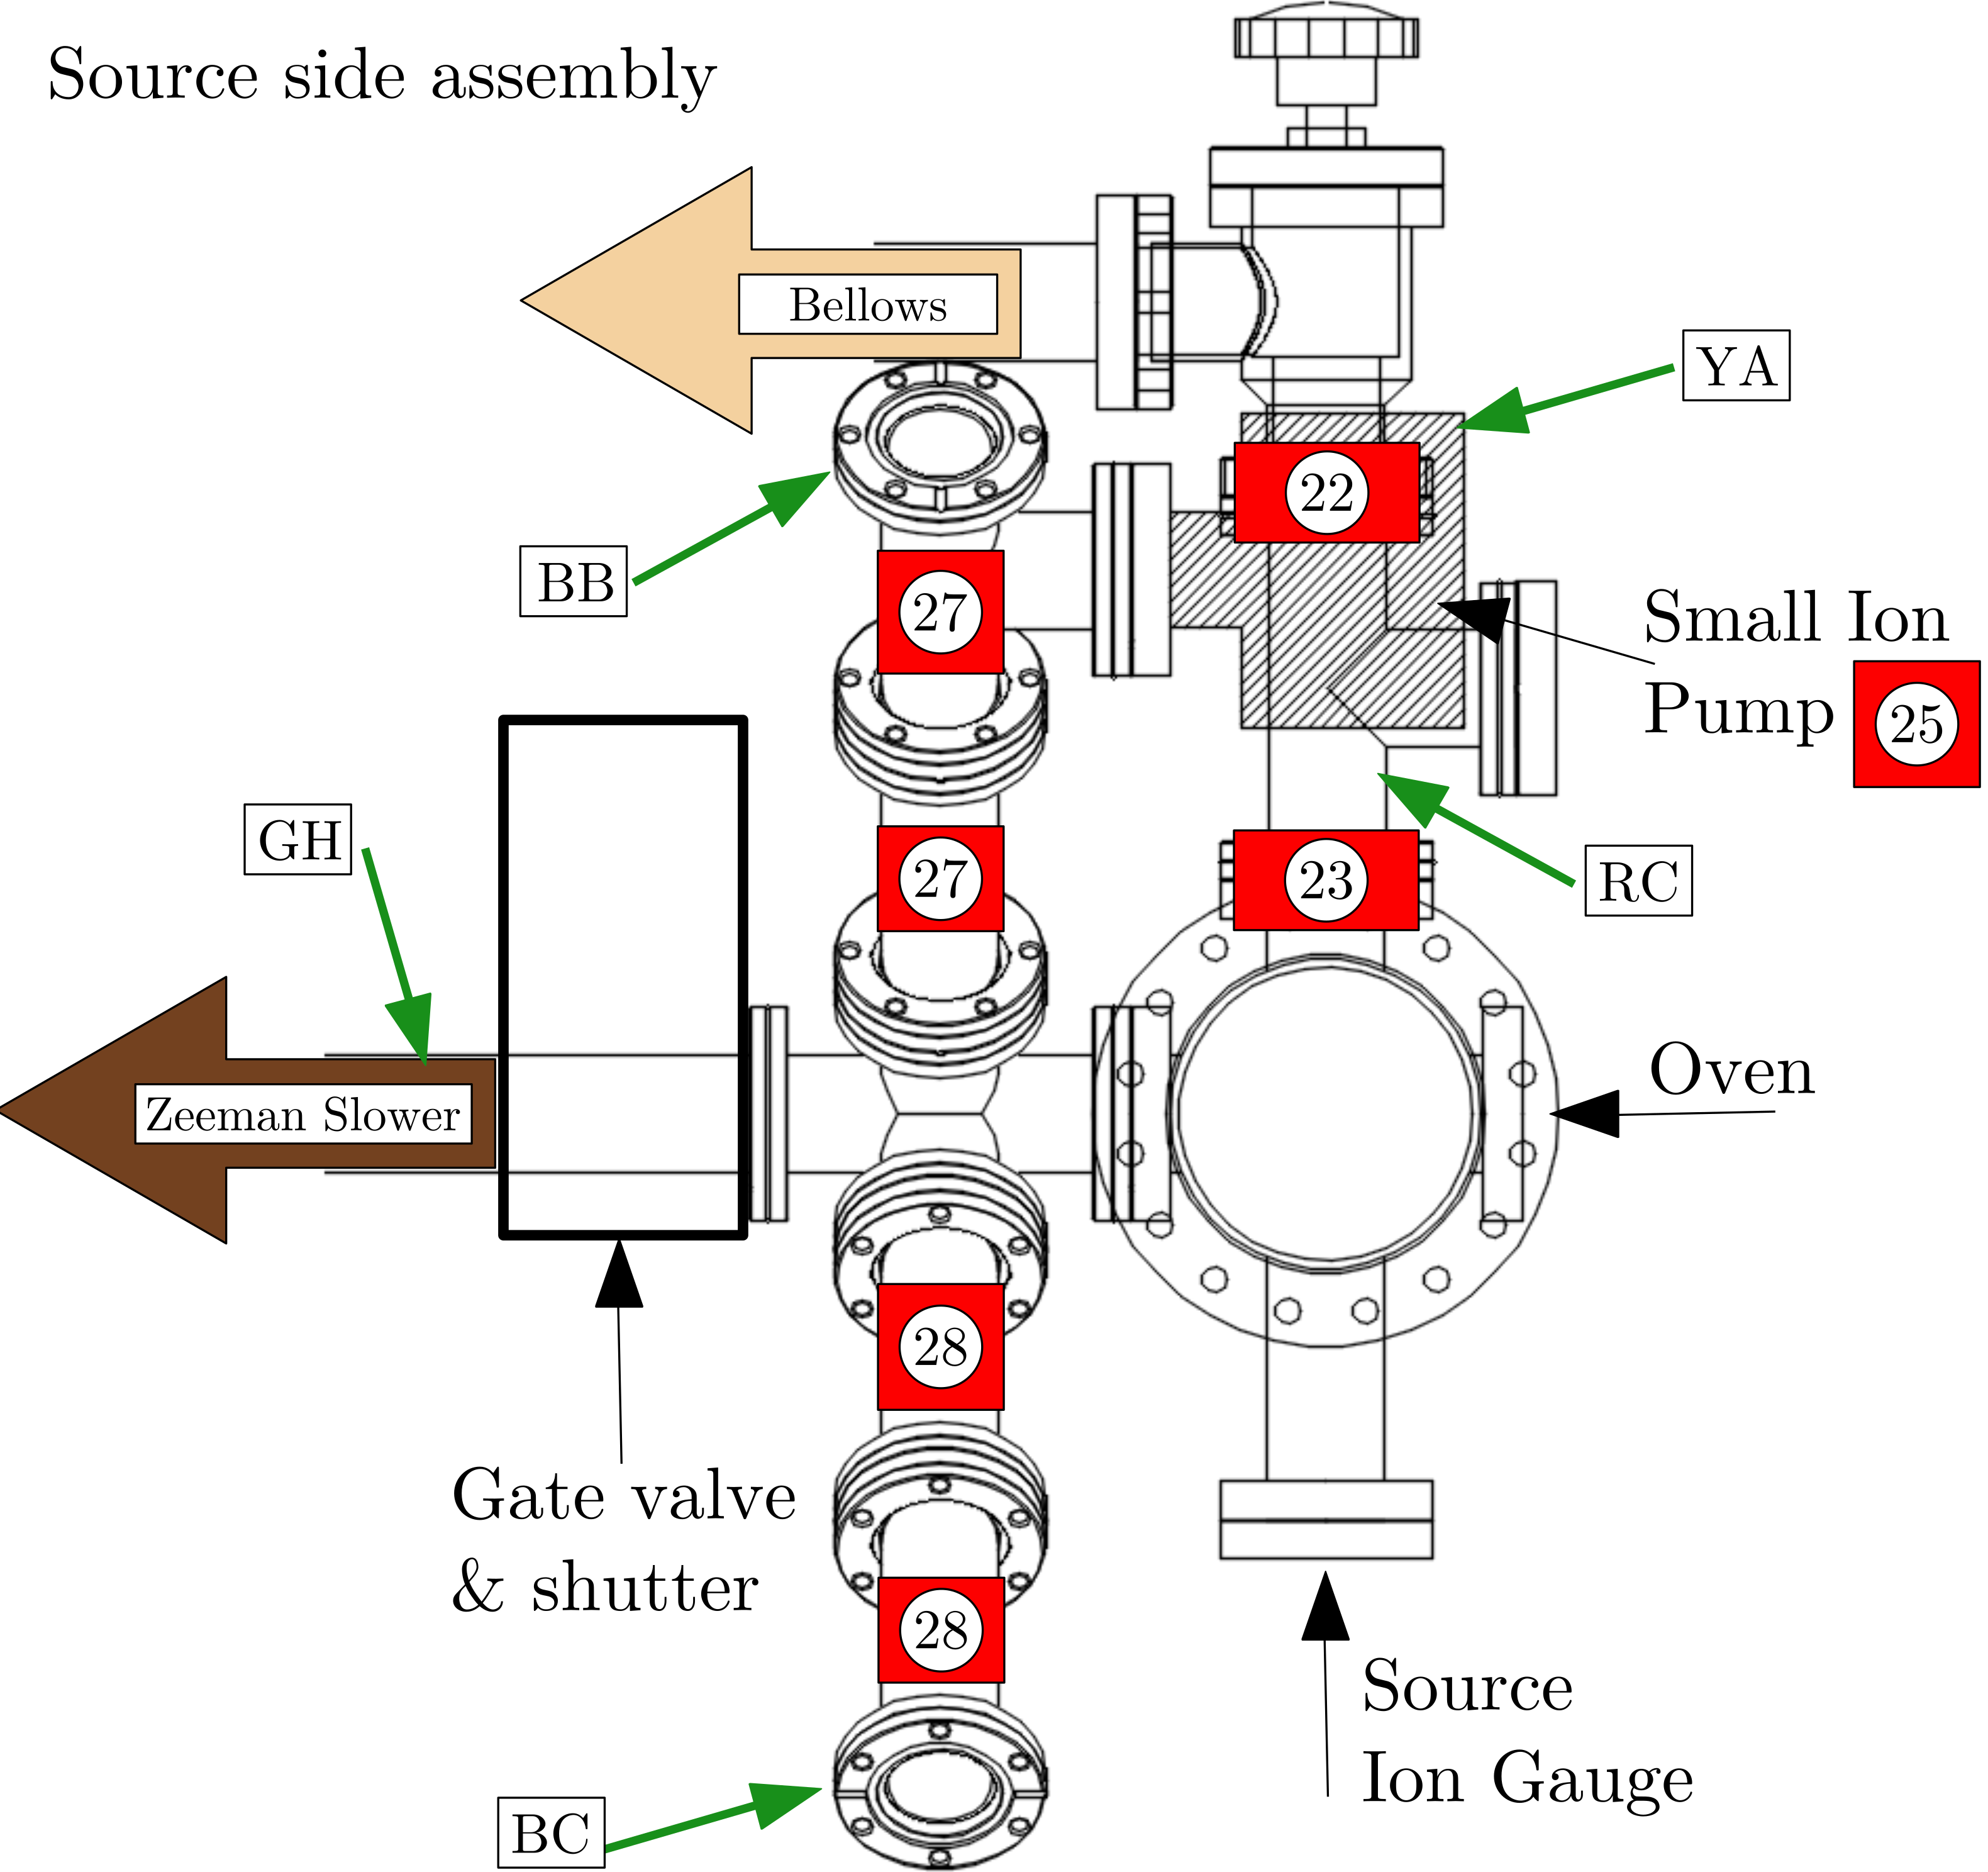
\includegraphics[height=0.4\textheight]{vacuum_source_assembly.png}}
		\caption{Source assembly - side view}
		\label{fig:sourceSideView}
	\end{figure}
	
	\begin{figure} 
		\centerline{
		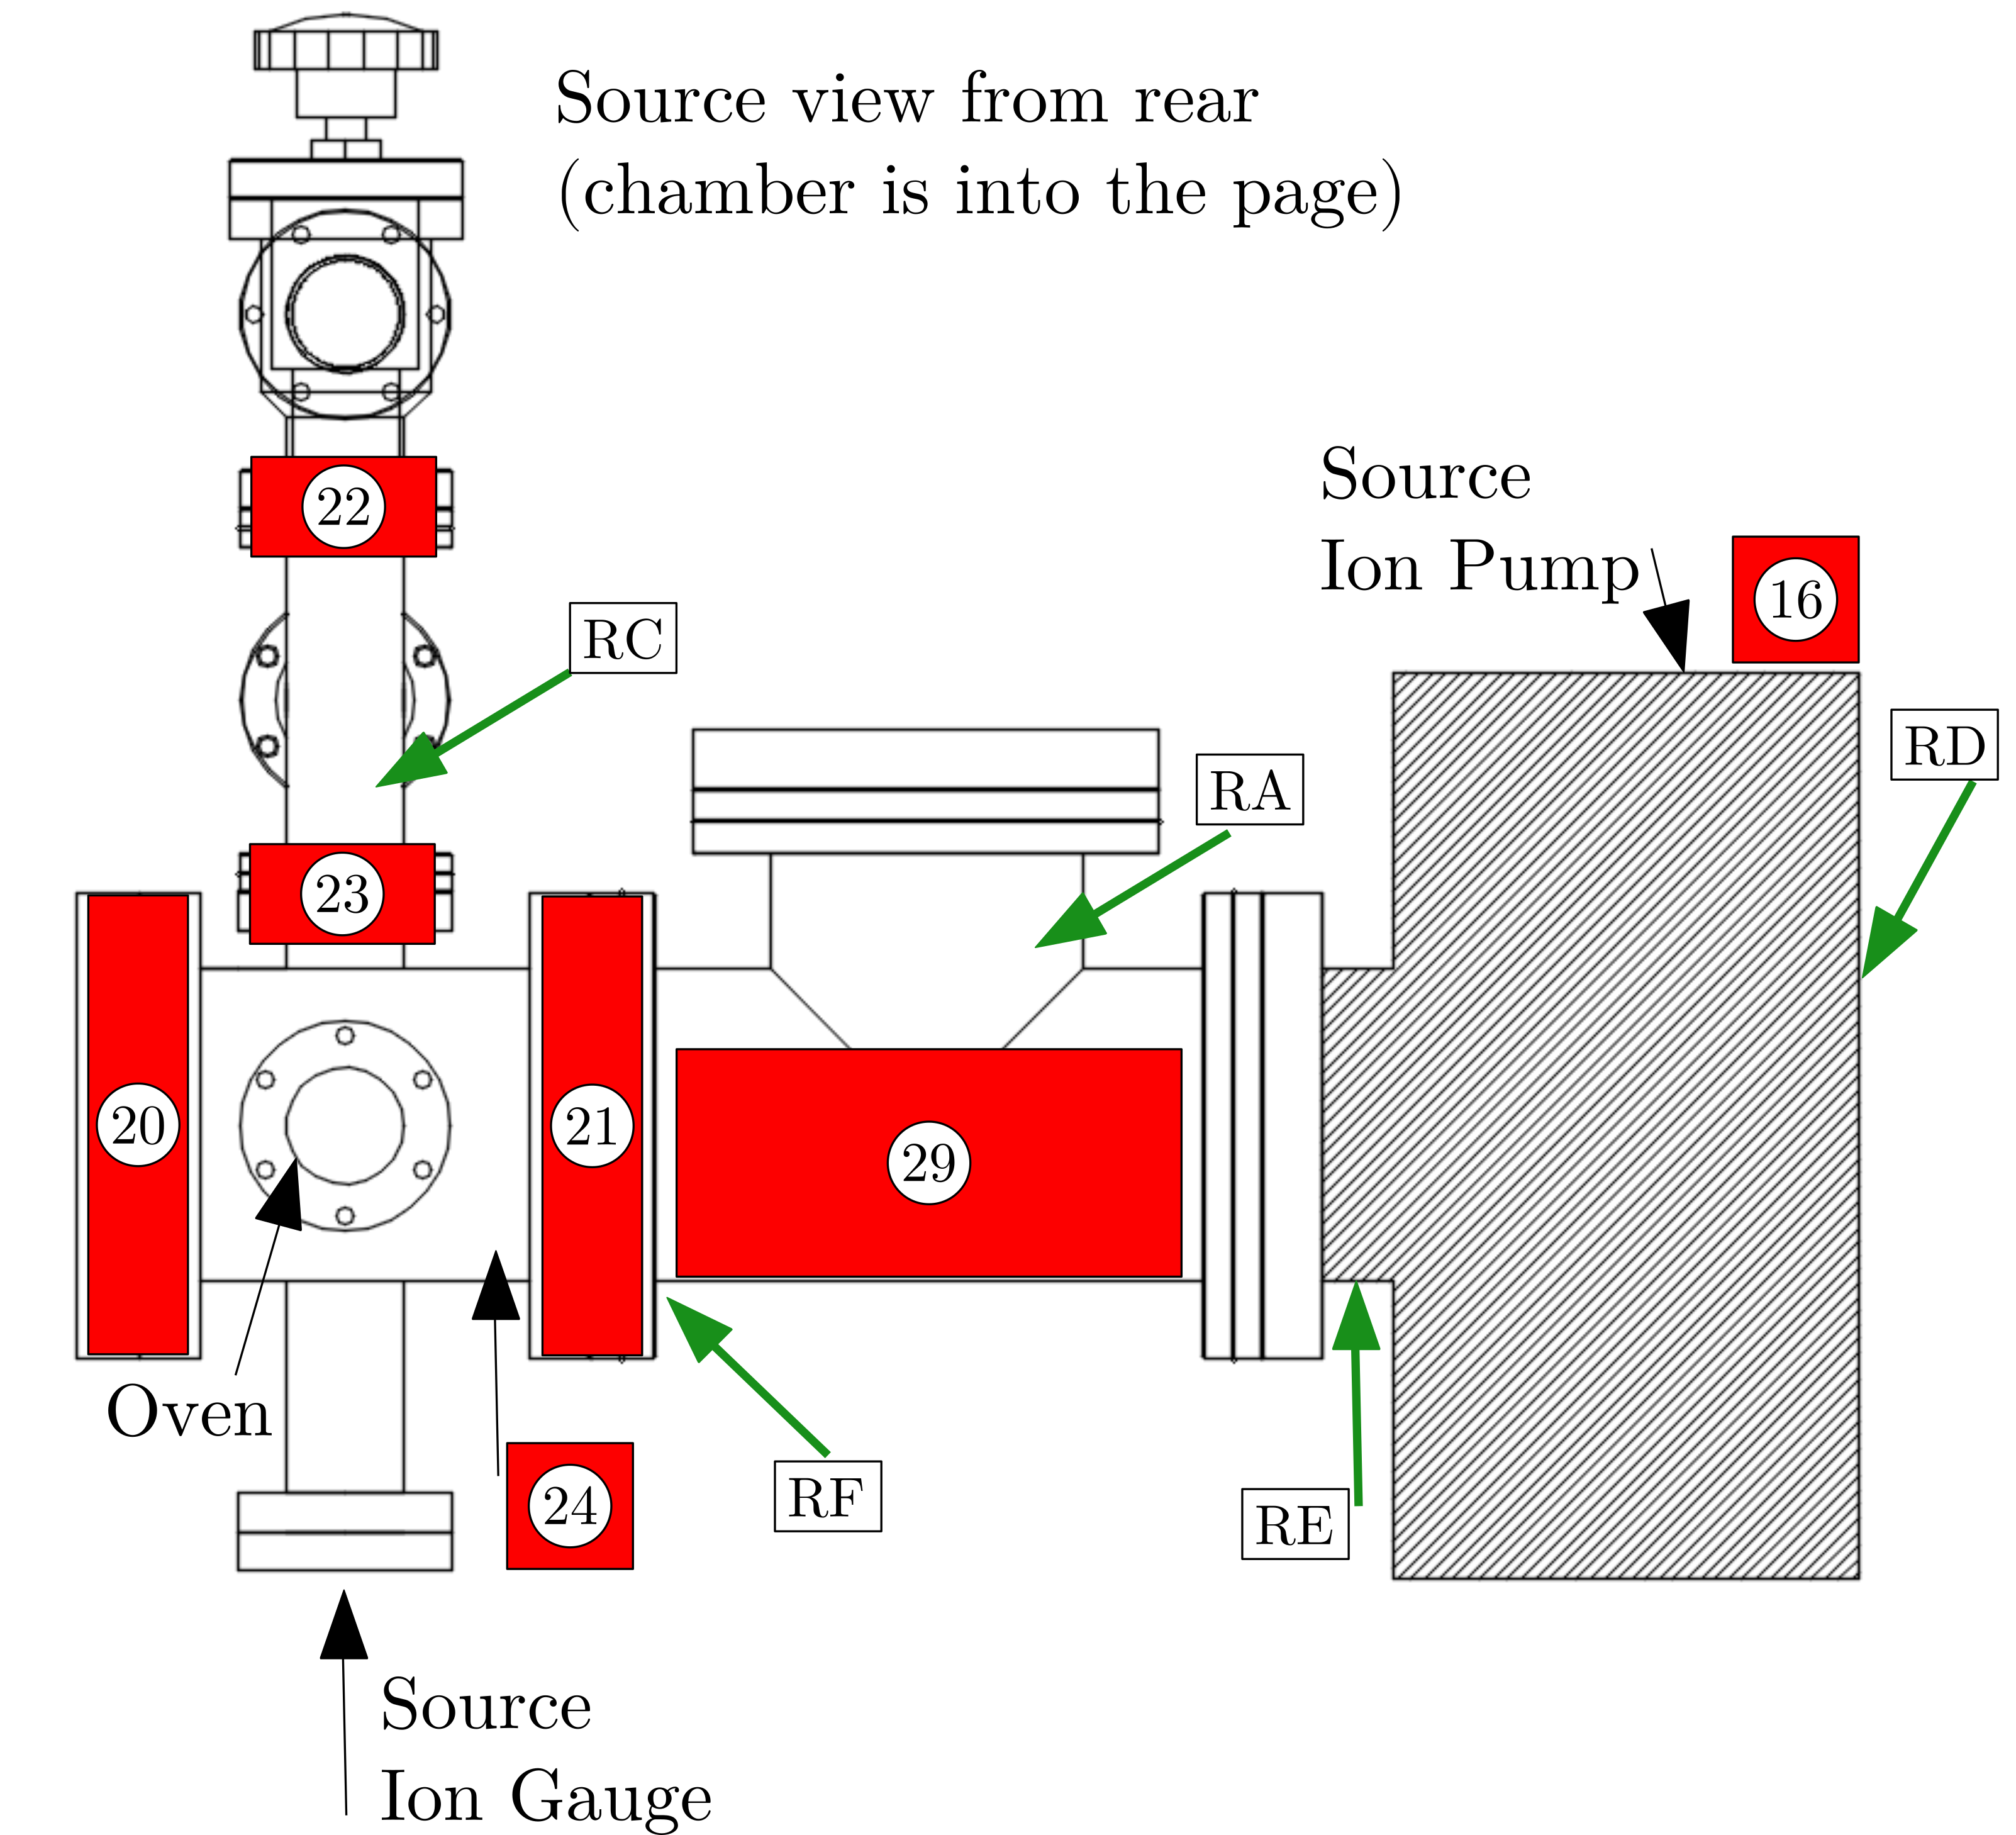
\includegraphics[height=0.4\textheight]{vacuum_source_rearView.png}}
		\caption{Source assembly - rear view}
		\label{fig:sourceRearView}
	\end{figure}
	
	\begin{figure} 
		\centerline{
		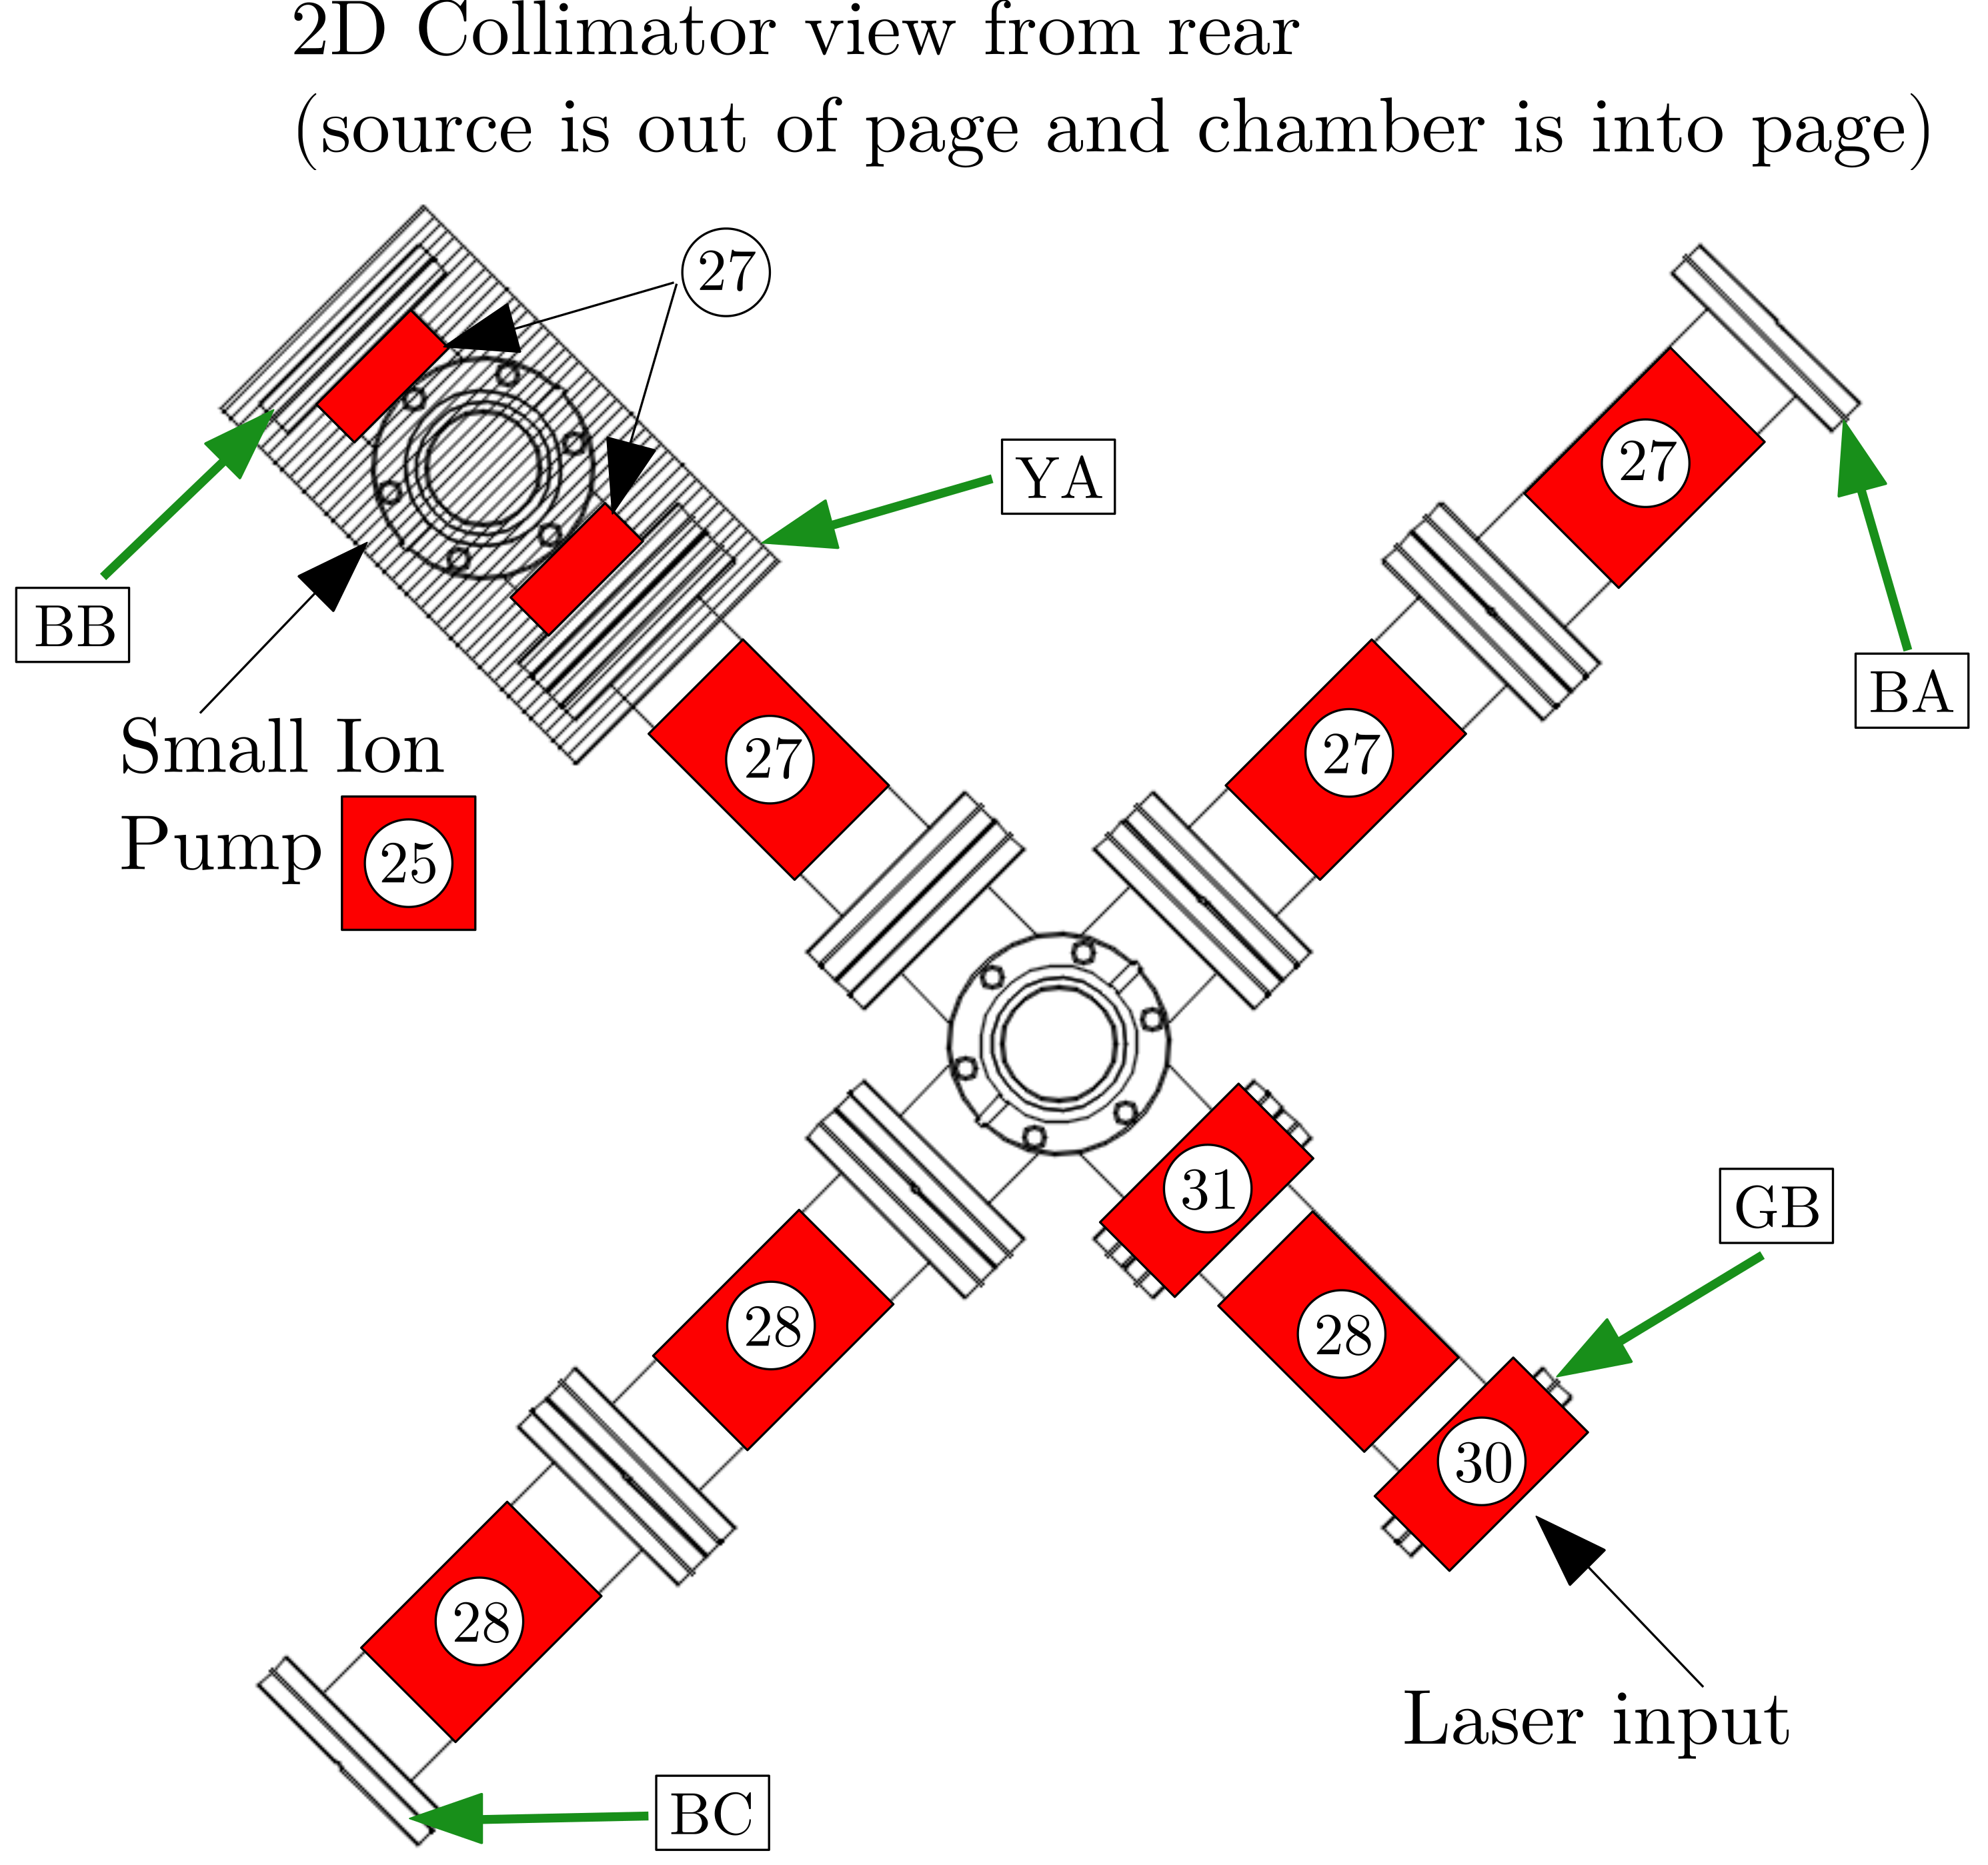
\includegraphics[height=0.5\textheight]{vacuum_2D_collimator.png}}
		\caption{2D collimator assembly}
		\label{fig:assembly_2Dcoll}
	\end{figure}
	
	\begin{figure} 
		\centerline{
		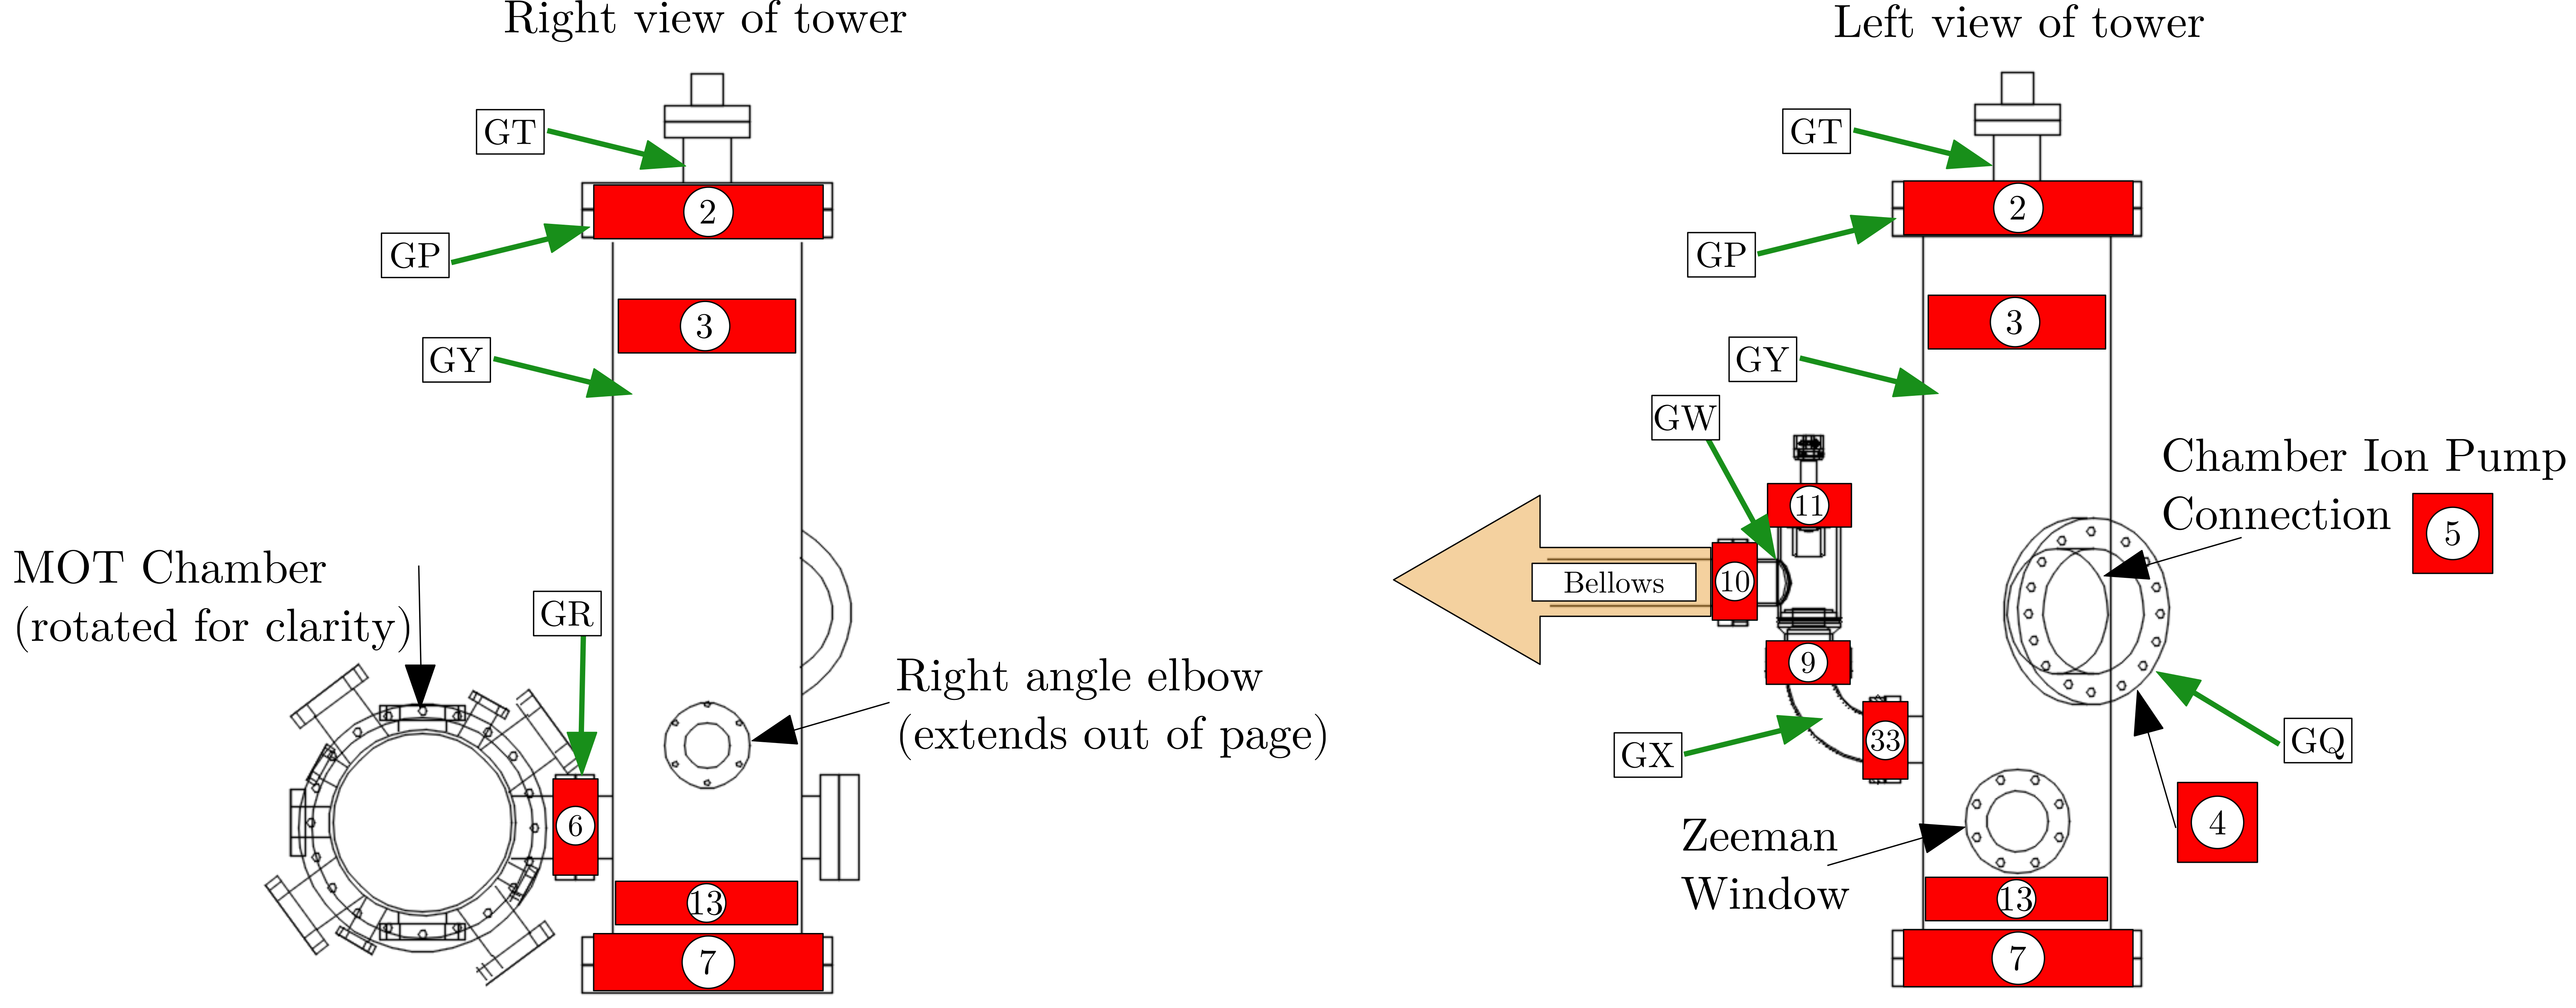
\includegraphics[width=1.25\textwidth]{vacuum_tower.png}}
		\caption{Cryo tower assembly}
		\label{fig:cryoTower}
	\end{figure}
From right to left, the system starts with an oven source based around a custom nozzle design which uses a rod heater to vaporize elemental strontium.
Next, there is a 6 way tee used for the optical molasses step which we refer to as the 2D collimator. 
From here atoms pass through a narrow differential pumping tube and into the entry port of the Zeeman slower where a majority of the laser cooling takes places as atoms traverse the 10.5\,inch one dimensional cooling stage. 
Following the Zeeman slower, atoms enter the science chamber where a plethora of lasers are used to manipulate and probe their behavior.
Chief among these laser systems are the MOT sequences and high intensity far off-resonant optical dipole traps used for the final stage of confinement.
Lastly, the body of the science chamber is supported by the cryo tower which houses a titanium sublimation catridge (model: Varian 916-0061 series) and is the entry point for the Zeeman laser.
It is worth explicitly noting that this Zeeman window is necessarily directly opposite the atomic source and therefore is subject to a flux of hot atomic strontium which will eventually coat the vacuum side. A brief note on a possible solution to this problem is explored at the end of this section.

While the source and science chamber have remained largely unchanged since the publication of Natali's thesis, several key improvements and events have occurred over the last few years\footnote{As of April 2019, the most up to date CAD drawing for the Neutral apparatus is located at \texttt{KillianDrobo:\textbackslash Neutral\textbackslash Laboratory Systems\textbackslash Vacuum Chamber\textbackslash Neutral Chamber\textbackslash 2017.12.26\_strontiumvacuum35\_latticetable.dwg}. Additionally, please consult the README file located in this folder for further information.}.
These differences will be the subject of our discussion in the latter part of this section.


% Orientation of lasers to chamber 
Fig \hl{something} shows a closer view of the science chamber and defines a coordinate system as well as directional labels used throughout this thesis. 
We will use this reference when illustrating the orientation of various lasers through the science chamber to help the reader.

The original drawings of these components can be found in App. A.10 of \cite{MartinezdeEscolar2010} along with detailed information on the window coatings.

\paragraph{Recent changes}
\subparagraph{Addition of platform:}
While exploring routes to produce quantum degenerate gases of strontium, it was determined that different geometries of traps were necessary to achieve efficient forced evaporation. 
The task of redesigning the optical dipole traps was undertaken by Ying Huang and is detailed in her master's thesis \cite{Huang2013}. 
As part of this project, a raised platform was designed and built around the chamber to facilitate beam shaping and launching of the ODT laser.
Details of the platform are available in the main apparatus CAD drawing.
%Unfortunately, while a major portion of this platform design is available in the main apparatus CAD file, the platform opposite of the oven is not documented.
%Nor is there a complete assembly drawing incorporating the chamber and platform, which may confound future efforts to build around the chamber as more complexity is introduced. 

The raised platform has become the primary method for directing lasers into the chamber including the 1064\,nm bulk optical dipole trap and the 532\,nm optical lattice, both of which are outlined below. 
During installation of the free space optical lattice we observed heating and hypothesized that relative movement of the platform and chamber may be a cause.
Supporting struts were then added beneath the chamber in an attempt to secure it to the platform around 2016.
However, the extreme sensitivity of cold atoms and occasional observation of shot to shot fluctuations persists the concern of relative movement between non-rigid components.

These concerns were reinforced when we observed increased stability with the addition of a partial cover over the platform optics for the optical dipole and lattice traps. 
Initially meant as an optical safety measure for enclosing the high power beams, the cover led to a marked decrease in shot to shot fluctuations of the cloud position after a time of flight.
With further testing we were able to attribute the increased stability to a mitigation of air currents caused by close proximity of the platform optics to the ventilation system meant to thwart dust accumulation inside the experimental enclosure.

% Running out of strontium
\subparagraph{Running out of strontium:}
In the winter of 2017 the neutral apparatus had been under vacuum for approx 8 years when suddenly we were no longer able to trap a significant number of atoms \footnote{It is was expected any trapping loss due to low strontium would be gradual and we were not able to determine the cause of the abrupt behavior.}.
After extensive testing, we hypothesized that we had run out of elemental strontium within the atomic source.
This led us to break vacuum, reload strontium, and perform a light bakeout procedure to reestablish the requisite ultrahigh vacuum for experiments.
Details of this bakeout procedure can be found in App. \ref{app:breakingVacuum}. 
Through this process we confirmed our hypothesis that lack of strontium was the cause of the issue. 
Figure \ref{fig:2d_coll_flourescence} shows the atom beam fluorescence after refilling the oven.
This image was taken while using the Zeeman laser to cause photon scattering and looking down the 2D collimator.
	\begin{figure}
		\centerline{
		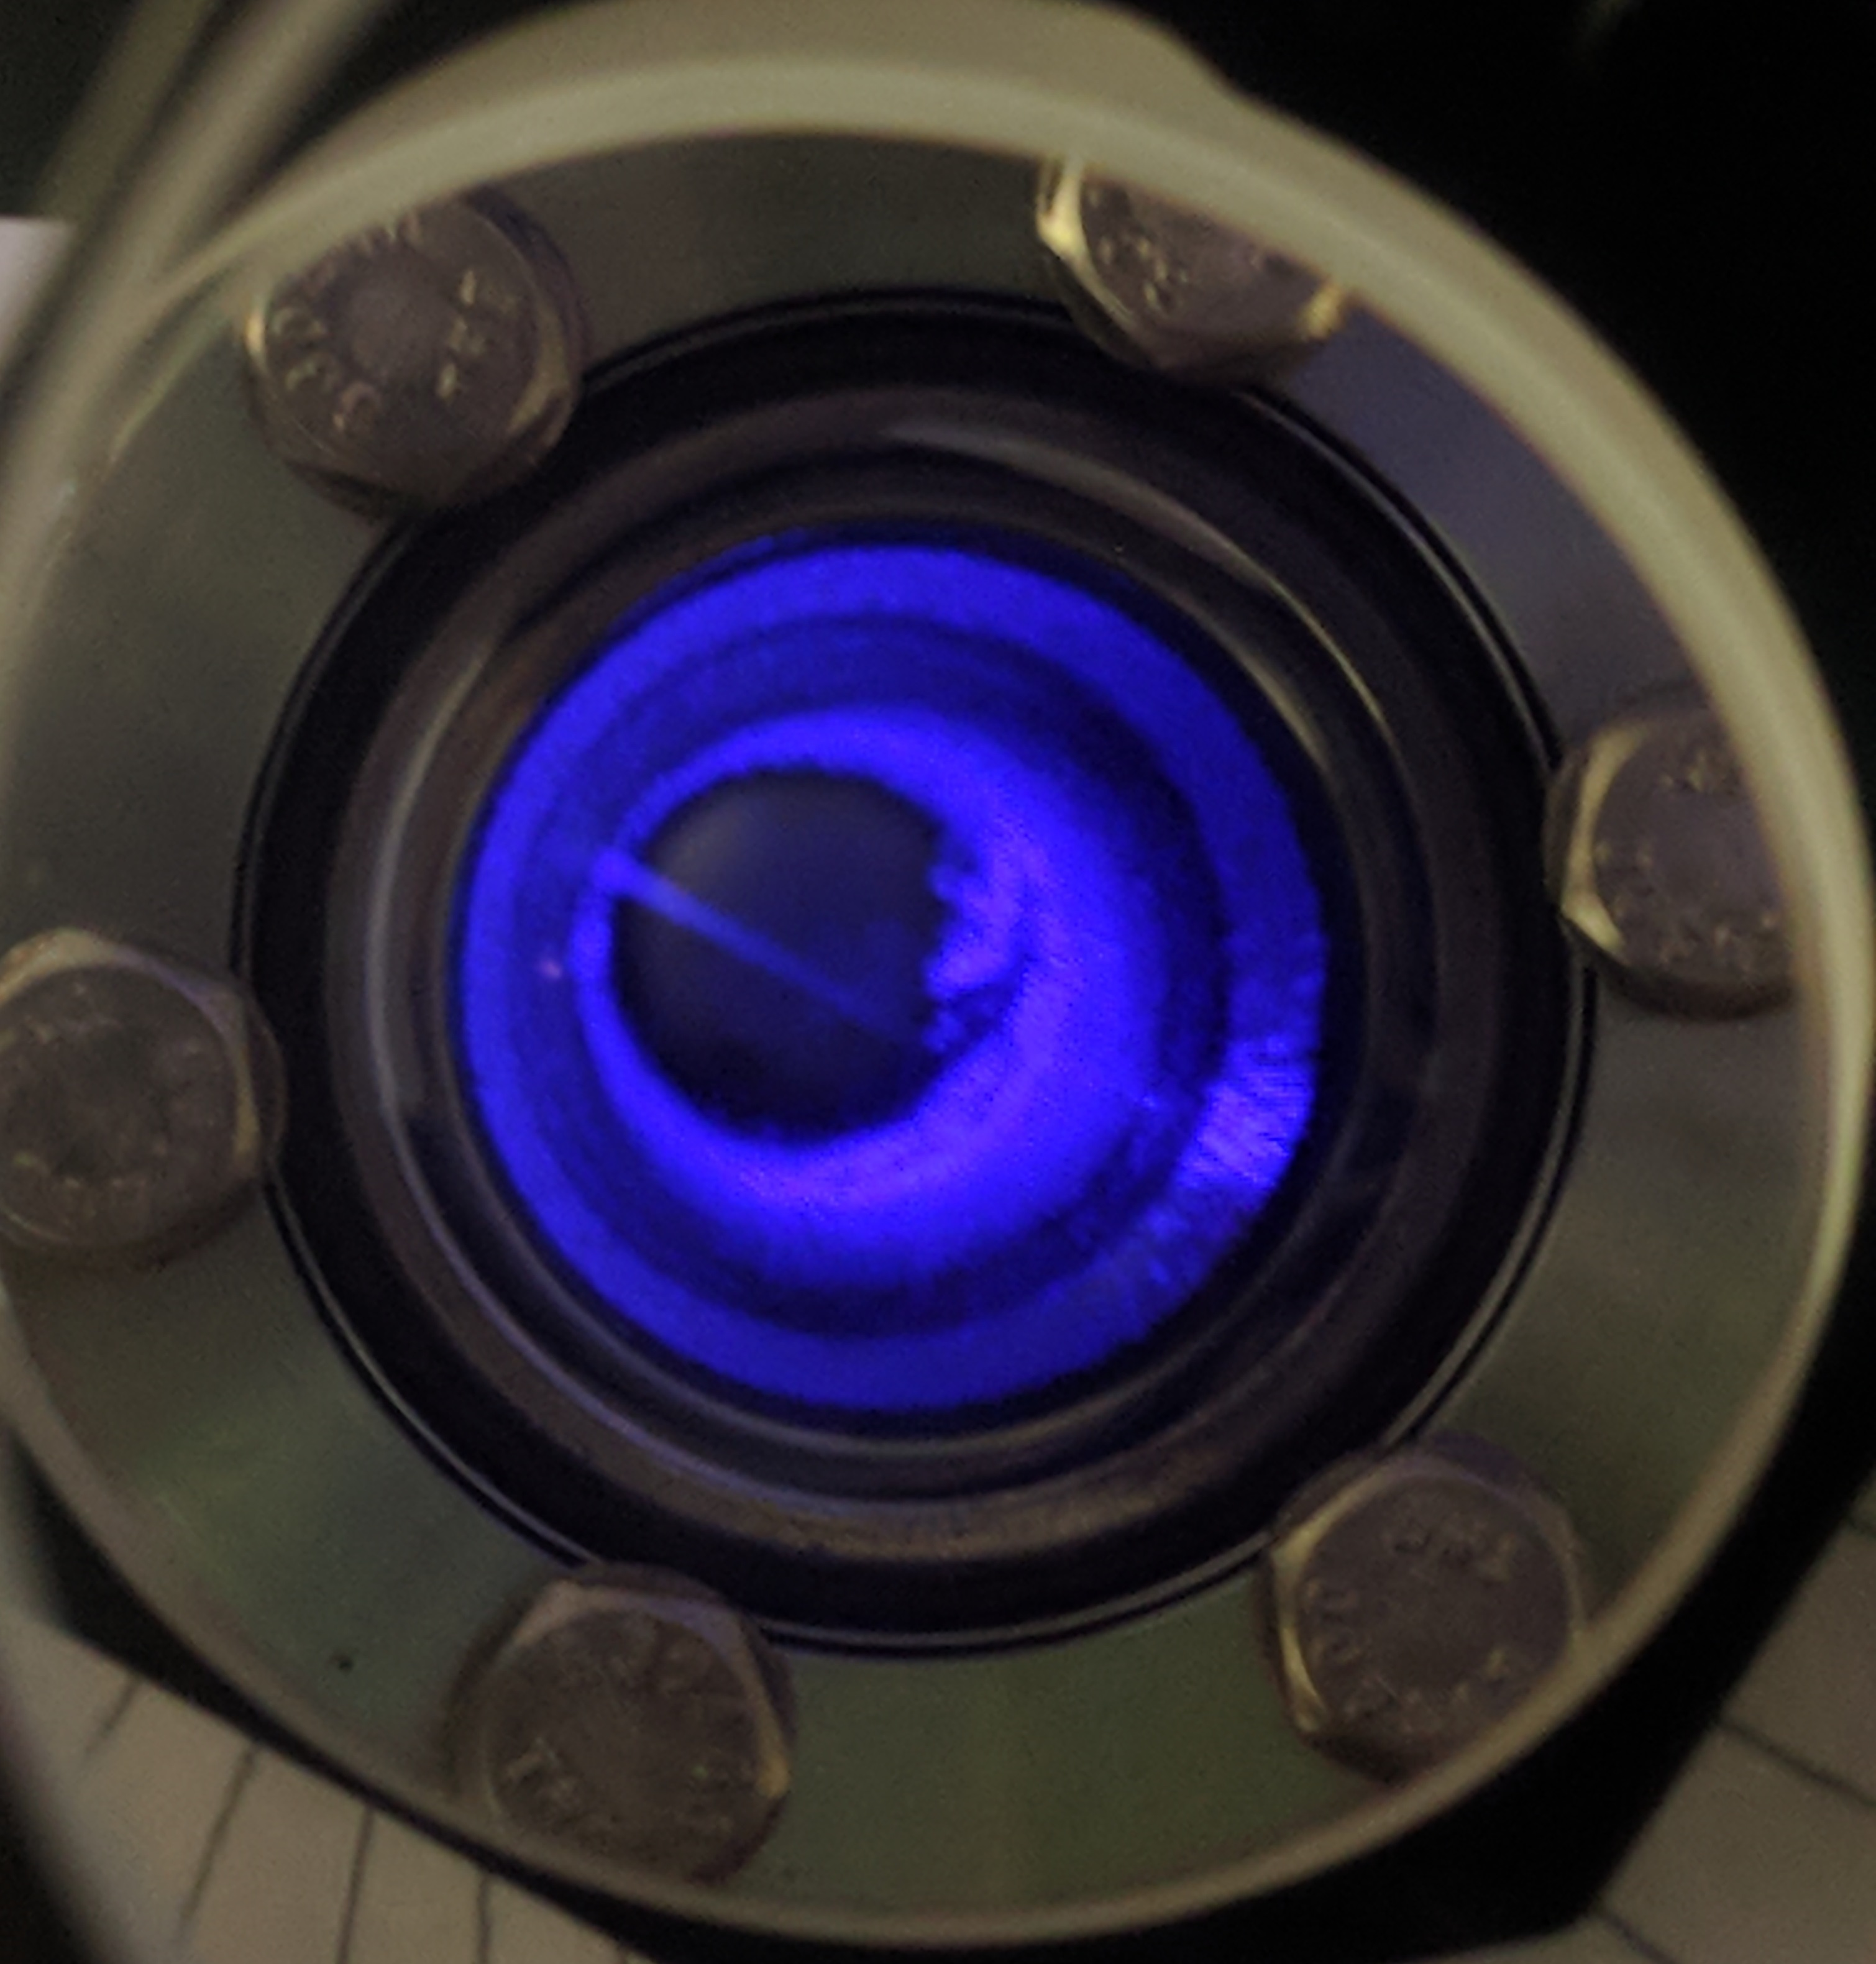
\includegraphics[height=0.5\textheight]{vacuum_IMG_20171103_184vacuum_230.jpg}}
		\caption{Typical fluorescence of Zeeman beam looking down 2D collimator}{This view is found using a 2 in mirror aligned along the path of the first pass of the 2D collimator and looking down the collimator tube. While looking at this angle, we are able to see the Zeeman beam move across the atom column when moving the last turning mirror. Reduction in this fluorescence signal from that shown was the primary indicator of lack of strontium in the source.}
		\label{fig:2d_coll_flourescence}
	\end{figure}  
Prior to this event the Neutral apparatus enjoyed lifetimes of approx. 25s as measured by background lifetimes measurements within the IR optical dipole trap. 
Approximately a year after restoring vacuum we have measured lifetimes on the order of 15s, the cause of the discrepancy is not rigorously known.

During the process of breaking vacuum we attempted several upgrades to the apparatus including adding a gate valve between the cryo tower and the Zeeman window and redesigning the atom nozzle source to incorporate a fixed heat shield around the heating element. 
Details of the nozzle design can also be found in App. \ref{app:breakingVacuum}.
Unfortunately, multiple issues arose during construction which led us to re-establish vacuum without these upgrades in place.
Therefore, they are documented in the appendices for potential future use.

Finally, after removing the atom oven to replace strontium, we placed a temporary viewport to facilitate alignment of the Zeeman beam through the length of the vacuum system. 
While aligning we observed an unexpected partial occlusion of the Zeeman beam and upon further investigation learned that the differential pumping tube is noticeably not parallel to the atom trajectory.
We were not able to determine the severity of the misalignment since the tube is not easily accessible and replacement is problematic as the tube is attached to a copper gasket held between flanges connecting the atom source chamber and the 6-way tee of the 2D collimator. 
The main readily measurable symptom is the occlusion of the Zeeman beam, which with an input power of approx. 120 mW before expansion optics and entering the chamber, only measures approx. 60 mW of transmitted power through the length of the vacuum system. 
A solution to bend the soft copper with a rod was proposed but abandoned due to concerns of cracking the thin copper.
As adequate repair of the tube necessitates a drastic and practically infeasible deconstruction of the vacuum system our goal here is to document the issue for future students.
It is currently hypothesized that this problem is the primary cause of the much longer load times needed in the Neutral apparatus compared to the newly designed Rydberg machine.

\paragraph{Clarifications from de Escobar thesis}
\subparagraph{HV version 1 \& 2:}
As a point of clarification, Natali's thesis \cite{MartinezdeEscolar2010} presents two versions of the HV chamber in figures A.42 - A.47 while referencing that the original construction proceeded with version 1. 
However, version 2 (the cryo tower) was installed around 2011 and is currently in use. Version 2 is shown in Fig.\,\ref{fig:cryoTower} and details are available in the apparatus CAD drawing.

\subparagraph{Collimating array in nozzle:}
% hypodermic needle nozzle
Once more, Natali's thesis refers to the installation of an improved nozzle design incorporating an array of collimating tubes constructed from 2$\mu$ hypodermic needles (model: \hl{find}). 
Modeling and construction of this design was done by Anton Mazurenko, \cite{Mazurenko2010}, with the goal of improving the angular discrimination of the oven assembly to produce a more highly collimated beam of atoms.
Figure \ref{fig:2010_nozzle} shows the improved nozzle design \footnote{For reference, this nozzle design is labeled "new nozzle summer 2010" in the apparatus CAD file to distinguish it from the other nozzle drawings also present.}.
	\begin{figure}
		\centerline{
		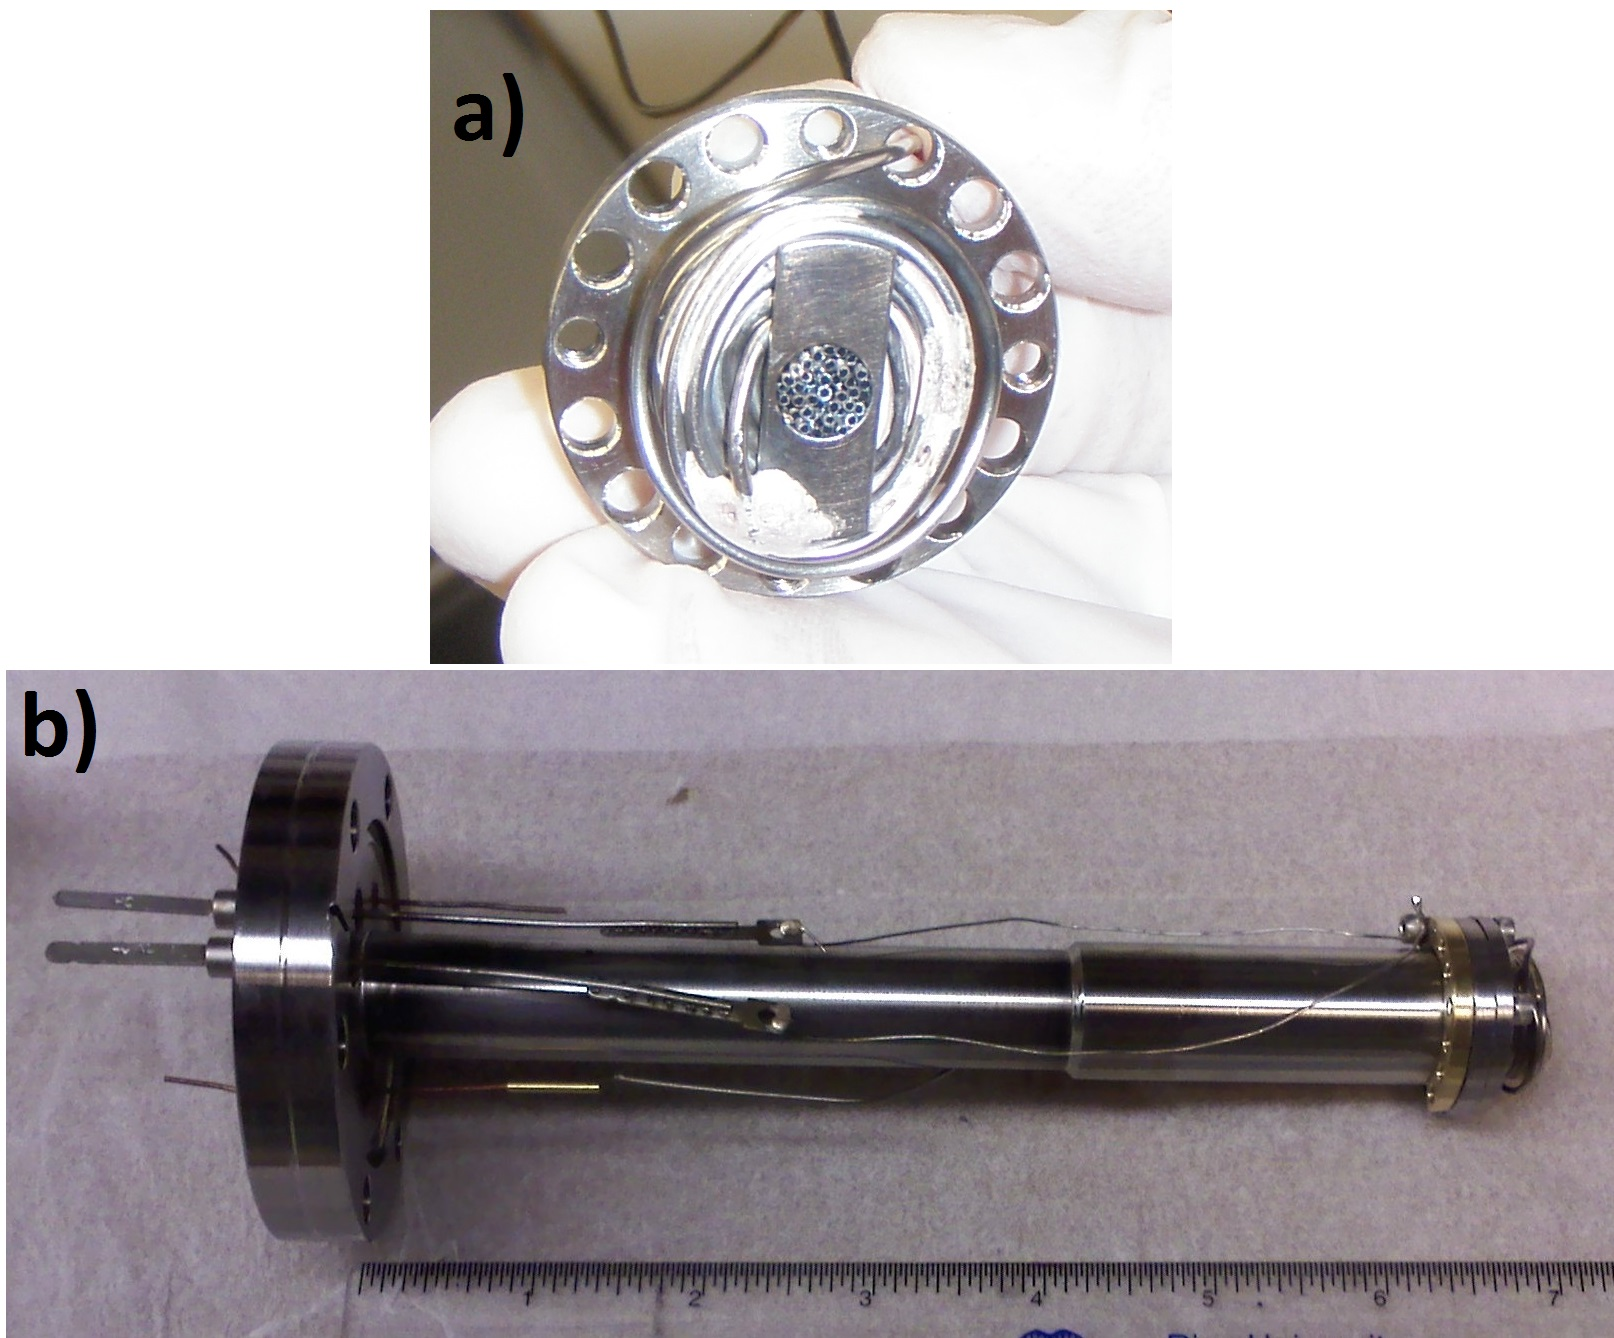
\includegraphics[height=0.4\textheight]{vacuum_nozzle.jpg}}
		\caption{Atom oven and nozzle construction}{a) The nozzle through which vaporized strontium enters the experiment. Here we see the array of collimating tubes behind which solid strontium is packed. b) The complete oven construction which houses the cartridge heater and the nozzle at the tip.}
		\label{fig:2010_nozzle}
	\end{figure}
The original assembly of this oven also incorporated a heat shield that would insert over the construction shown in Fig.\,\ref{fig:2010_nozzle}b) but this shield is not currently installed on the source oven.
%was ultimately abandoned since there was no way to fasten it to the flange which led the shield to fall off. 
 
\paragraph{Ablating strontium off window} \label{p:ablatingSr}
While not directly related to any experiment or typical procedure, this sub-section summarizes a brief side project of using a pulsed 532\,nm Verdi to ablate strontium from a vacuum window.
As discussed previously, a common problem faced by strontium experiments is the accumulation of strontium on the Zeeman entry port. 
These deposits may then act as a partial mirror leading to attentuation of the crucially important Zeeman beam. 
It was shared through private communication with professor Killian that pulsed 532\,nm light (such as from a q-locked Verdi system used in the Plasma laboratory) might vaporize the strontium off the window and restore any loss in transmitted Zeeman power. 
Using a test apparatus we were able to verify that indeed we could ablate the strontium off of an uncoated window, as shown in figure \ref{fig:ablating_strontium}.
	\begin{figure}
		\centerline{
		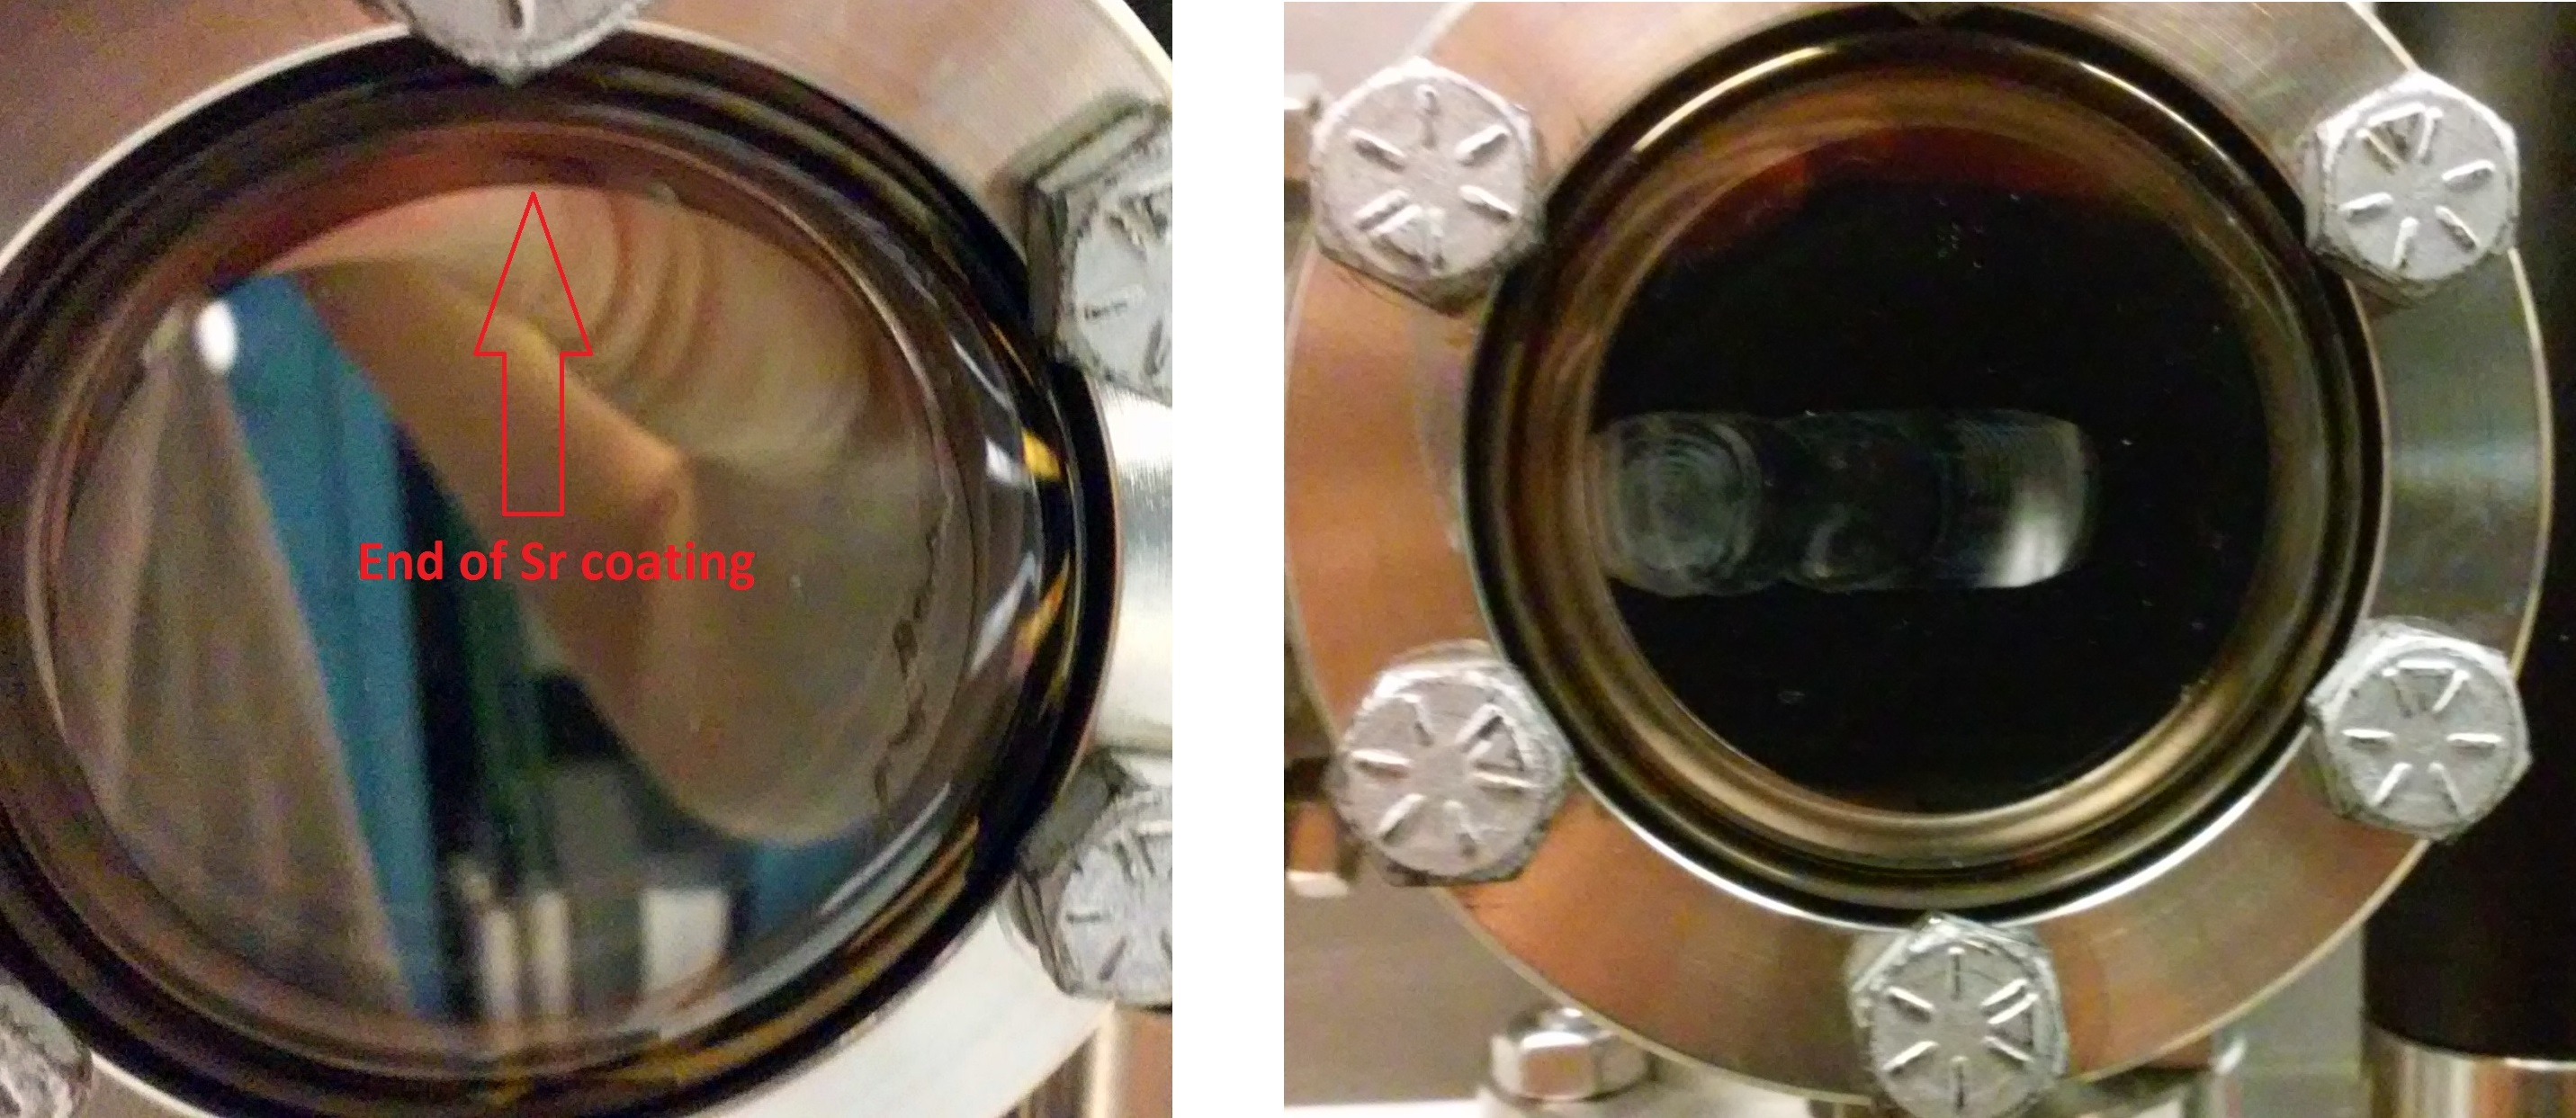
\includegraphics[width=0.8\textwidth]{vacuum_ablated_sr2.jpg}}
		\caption{Ablating strontium coating from window}{Comparison of the before (left) and after (right) when using a pulsed 532\,nm Verdi to ablate strontium. The residue visible in the after image we hypothesize to be caused by high pulse energy. We reduced the pulse energy as we moved towards the center of the window.}
		\label{fig:ablating_strontium}
	\end{figure}
This promising test led us to install an optical traversal port connecting the Plasma and Neutral labs. 
Unfortunately, while flashing the Verdi on a small section of the Neutral Zeeman window we found that the energy needed to ablate the strontium was accompanied by deformation of the window.
We discontinued the ablation upon observing this behavior to avoid further damage and we subsequently replaced the window after breaking vacuum as previously noted.

In an effort to mitigate the time the window is exposed to the hot strontium beam, we have also installed a small servo motor to drive the atom shutter valve and integrated this mechanism into the experimental runtime. 
This integration only opens the shutter during times of actively trapping atoms. 
Details of the servo motor trigger integration into the neuKLEIN control system are available in App \hl{somewhere}.

\pagebreak
\section{Laser systems}\label{sec:laser_systems}
\setcounter{footnote}{0}
The heart of any atomic physics experiment are the laser systems which are the basis for laser cooling and various probes.
Our lab has transitioned to mainly using diode lasers and relies heavily upon the use of injection locked master - slave setups. \hl{ref}
Below we will outline the specifics of our light generation systems.
In particular, future experiments on the Neutral apparatus aim to explore quantum magnetism using strontium 87 and as such we will emphasize several key changes which have been made to the 461 locking and 689 trapping systems to facilitate these experiments.

\subsection{Wideband cooling stage: 461\,nm} \label{ssec:461sys}
\subsubsection{Overview}
As discussed in the experimental overview, the majority of our laser cooling is done using 461\,nm light. 
We generate and control these photons by amplifying and frequency doubling 922\,nm light from a master ECDL diode laser. 
Fig.\,\ref{fig:461blockSys} shows an overview of how we generate and use the 461\,nm light.
We will explore each of these sections in detail below, with emphasis on the MOT sub-system since it is the basis for many different components of the overall 461 generation.
	\begin{figure}
		\centerline{
		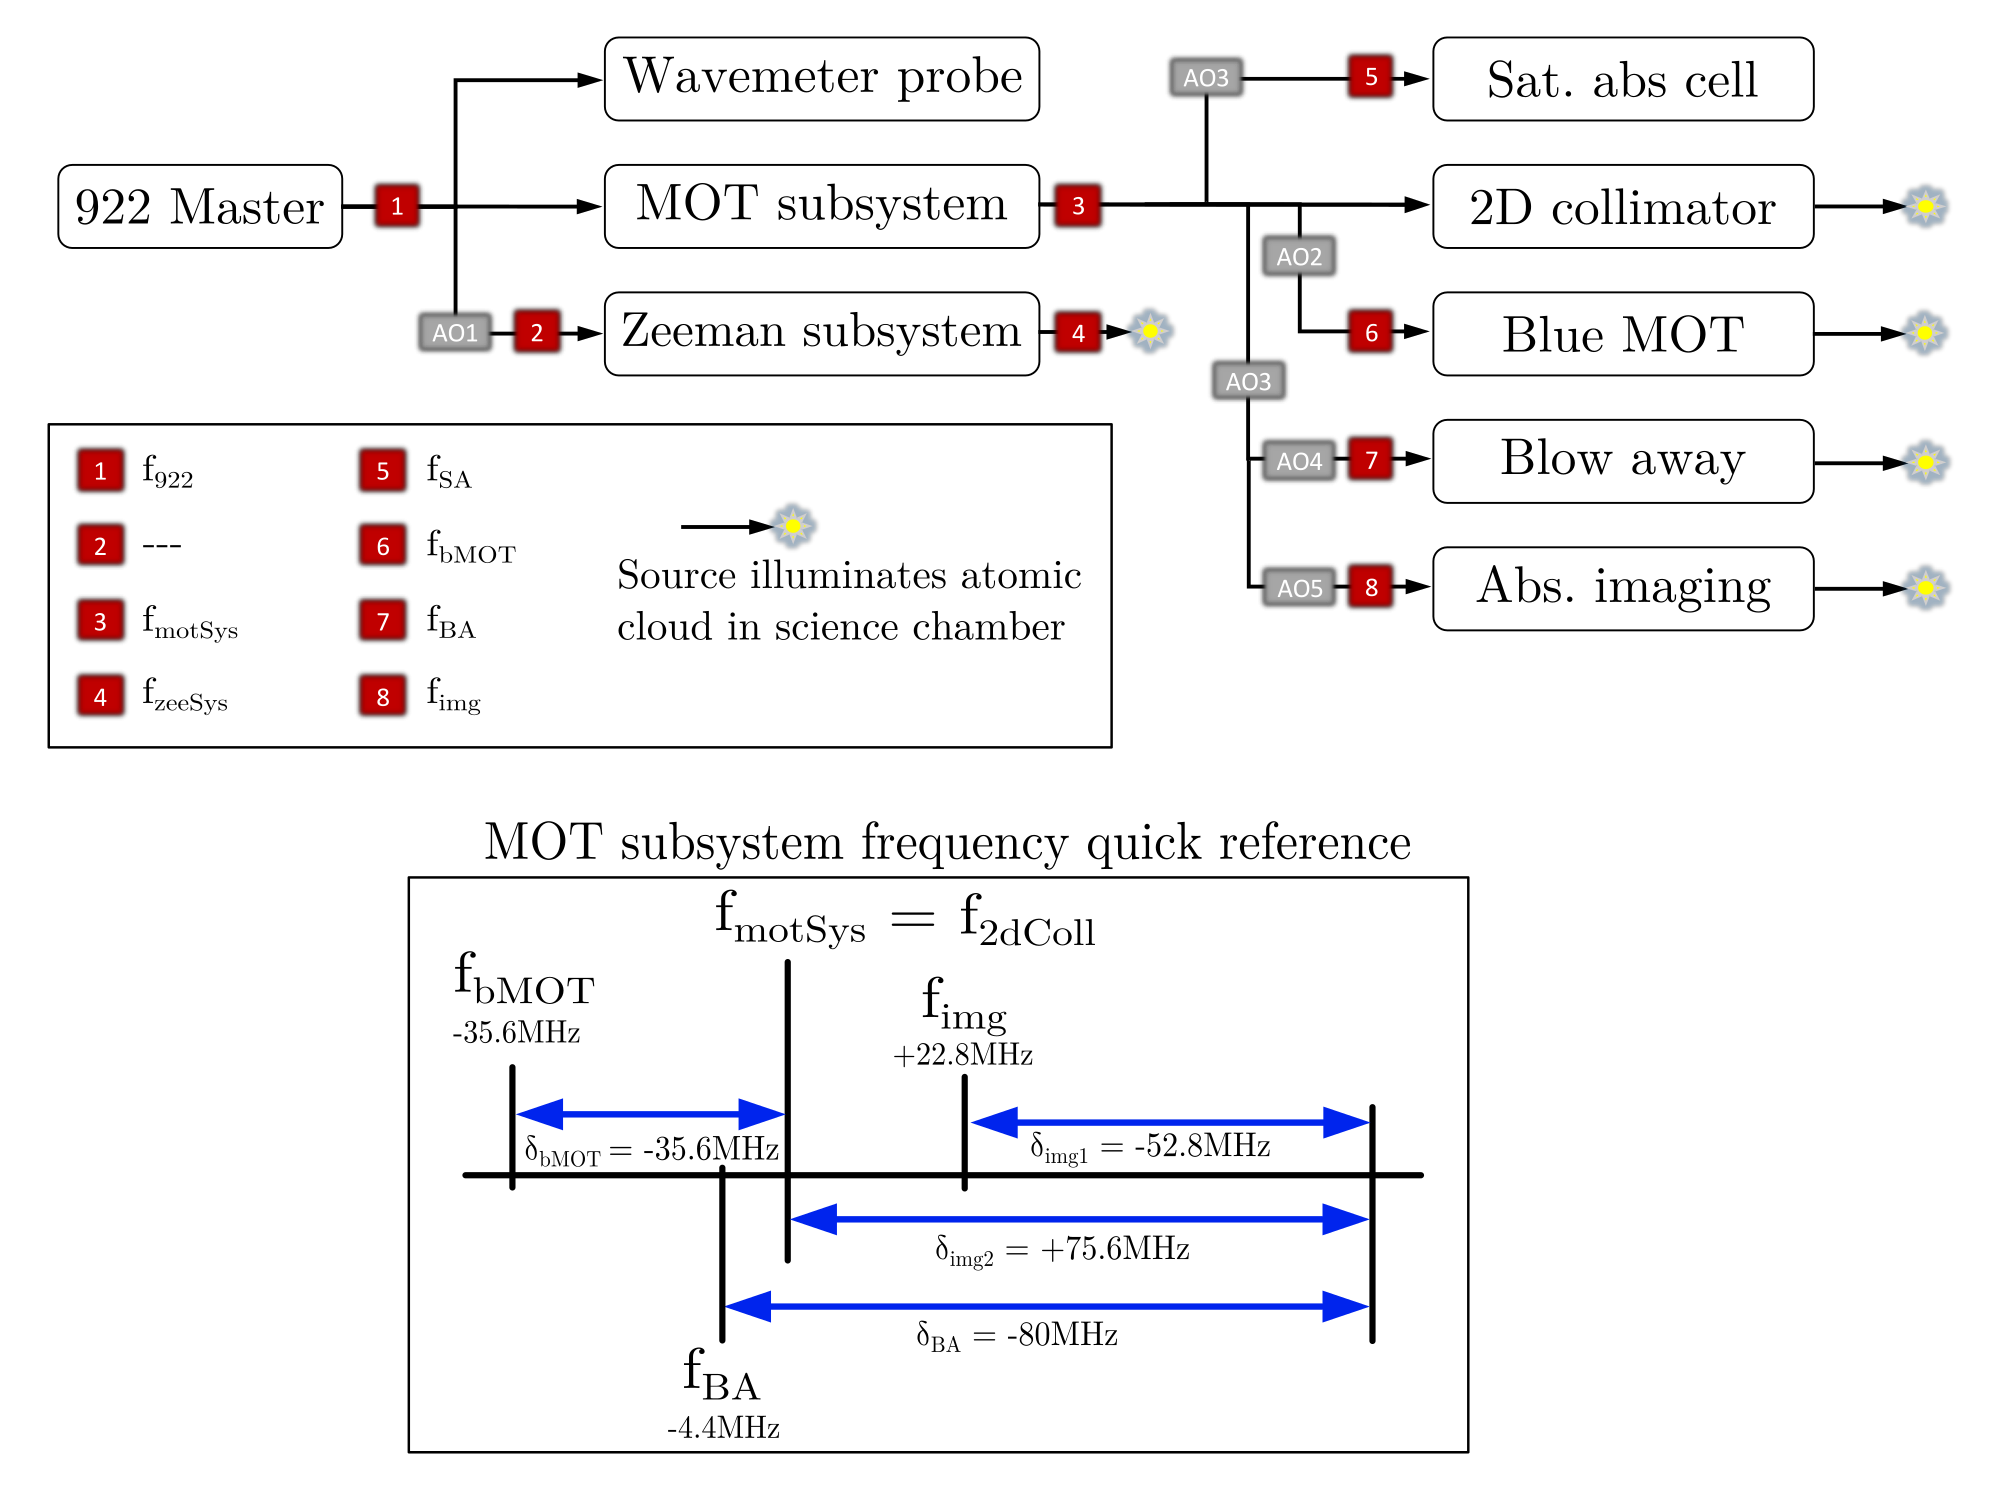
\includegraphics[width=\textwidth]{461_blueSystem.png}}
		\caption{461\,nm light generation system}{Top - Block schematic showing the relations of the various systems, AOMs, and frequencies used to lock the system for 461\,nm trapping and spectroscopy. See Table \ref{tab:461AOM} for information on the AOMs. Bottom - Relative frequencies of the MOT subsystem at various stages of the 461 system. Frequencies are quoted with respect to f$_{\text{motSys}}$ which in turn is controlled via the tunable sat. abs. to address different isotopes.}
		\label{fig:461blockSys}
	\end{figure} 

In conjunction with the block diagram, Table \ref{tab:461AOM} shows the details of the frequency shifts and AOM details. 
The position of these AOMs is represented by the numbered black circles while the labeled red squares define the various system frequencies.
The primary frequency relations for trapping and imaging are schematically represented in the lower portion of Fig.\,\ref{fig:461blockSys} and are determined via Eq. \ref{eq:461freqs}.
Table \ref{tab:461AOM} defines the shift variables used in these equations.
\begin{landscape}
\begin{table}[]
\centerline{
\begin{tabular}{@{}|l|c|c|c|c|l|l|l|@{}}
\toprule
\multicolumn{1}{|c|}{\textbf{Label}} & \textbf{Ind.} & \textbf{System} & \textbf{\begin{tabular}[c]{@{}c@{}}Shift\\ variable\end{tabular}} & \textbf{\begin{tabular}[c]{@{}c@{}}Nominal \\ Freq. {[}MHz{]}\end{tabular}} & \multicolumn{1}{c|}{\textbf{Freq. Source}} & \multicolumn{1}{c|}{\textbf{Freq. control}} & \multicolumn{1}{c|}{\textbf{AOM Model}} \\ \midrule
Zeeman & AO1 & 922 master & $\delta_{zeeman}$ & -252.4 & \begin{tabular}[c]{@{}l@{}}Mini Circuits\\ ZOS-300\end{tabular} & Static voltage & \begin{tabular}[c]{@{}l@{}}Crystal Tech. \\ 3200-1113\end{tabular} \\ \midrule
Blue MOT & AO2 & MOT & $\delta_{bMOT}$ & -35.5 & \begin{tabular}[c]{@{}l@{}}Mini Circuits\\ ZOS-50\end{tabular} & Static voltage & \begin{tabular}[c]{@{}l@{}}IntraAction \\ AOM-402A1\end{tabular} \\ \midrule
Image 2 & AO3 & \begin{tabular}[c]{@{}c@{}}Abs. imaging\\ \& Blow away\end{tabular} & $\delta_{img2}$ & +75.6 & \begin{tabular}[c]{@{}l@{}}Mini Circuits\\ ZOS-75+\end{tabular} & Static voltage & \begin{tabular}[c]{@{}l@{}}IntraAction \\ ATM-1001A1\end{tabular} \\ \midrule
Image 1 & AO4 & Abs. imaging & $\delta_{img1}$ & -52.8 & \begin{tabular}[c]{@{}l@{}}Mini Circuits \\ ZOS-150\end{tabular} & Static voltage & \begin{tabular}[c]{@{}l@{}}IntraAction \\ AOM-602A1\end{tabular} \\ \midrule
Blow away pulser & AO5 & Blow away & $\delta_{BA}$ & -80 & \begin{tabular}[c]{@{}l@{}}IntraAction \\ ME-801T7\end{tabular} & Internal synth. & \begin{tabular}[c]{@{}l@{}}IntraAction \\ ATM-802DA1\end{tabular} \\ \midrule
Sat. abs. shifter & AO6 & Sat. abs & $\delta_{SA}$ & +317.3 & \begin{tabular}[c]{@{}l@{}}Mini Circuits \\ ZOS-400+\end{tabular} & Static voltage & \begin{tabular}[c]{@{}l@{}}Crystal Tech. \\ 3200-141\end{tabular} \\ \bottomrule
\end{tabular}
}
\caption{461\,nm systen AOM details}{Ind. labels the AOMs as shown in Fig.\,\ref{fig:461blockSys}. The sign of the nominal freq. indicates the AOM order used.}
\label{tab:461AOM}
\end{table}
\end{landscape}

\begin{align} \label{eq:461freqs}
	&f_{\text{motSys}}  = 2f_{922}          & &f_{\text{zeeSys}}  = 2(f_{922} + \delta_{\text{zeeman}}) \nonumber \\
	&f_{\text{2dColl}}  = f_{\text{motSys}} & &f_{\text{bMOT}}    = f_{\text{motSys}} + \delta_{\text{bMOT}} \nonumber \\
	&f_{\text{img}}     = f_{\text{motSys}} + \delta_{\text{img2}} + \delta_{\text{img1}} & &f_{\text{SA}} = f_{\text{motSys}} + \delta_{\text{SA}} \nonumber \\
	&f_{\text{BA}}      = f_{\text{motSys}} + \delta_{\text{img2}} + \delta_{\text{BA}}
\end{align}

Overall frequency control, $f_{922}$, is determined via the magnetically tunable saturated absorption cell.
The use of magnetic tunability to control the 461\,nm light frequency is well documented in section 2.2.1 of Natali's thesis \cite{MartinezdeEscolar2010} and section 2.1.1 of Pascal's thesis \cite{Mickelson2010b}.
A more recent undergraduate project also explored optimizations of this scheme for the Rydberg apparatus \cite{MichaelViray2014}.

\subsubsection{922\,nm master}
The master 922 laser is derived from Sacher Lynx 922\,nm IR diode laser in a Littrow ECDL configuration.
Fig.\,\ref{fig:922optical}, shows a simplified optical schematic and Table \hl{some} gives typical running characteristics.
	\begin{figure}
		\centerline{
		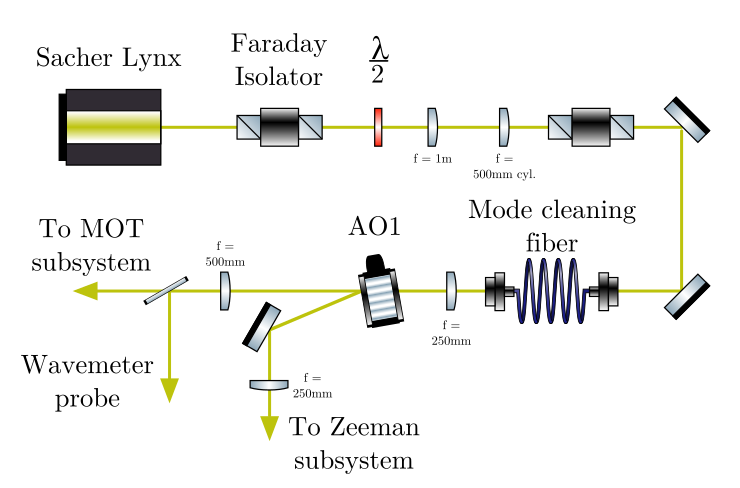
\includegraphics[width=\textwidth]{461_922schematic.png}}
		\caption{922\,nm master optical schematic}
		\label{fig:922optical}
	\end{figure} 
	
Starting at the master output, the beam is shaped and sent through a two optical isolators before it is coupled into an optical fiber.
The fiber output immediately goes through an AOM which detunes the diffracted order by approx. 250 MHz.
The diffracted and zeroth order are then separated with the unshifted beam sent towards the MOT generation subsystem and the shifted light towards the Zeeman subsystem.
We find it necessary to include dual isolators in front of the master laser and have found that inadequate alignment of these isolators can lead to significant instability in the frequency of the master which in turn may lead the doubling cavities to be unable to maintain a lock.

Fig.\,\ref{fig:922cavityLock} shows a simplified schematic of the negative feedback path for stabilizing the length of the doubling cavities.
	\begin{figure}
		\centerline{
		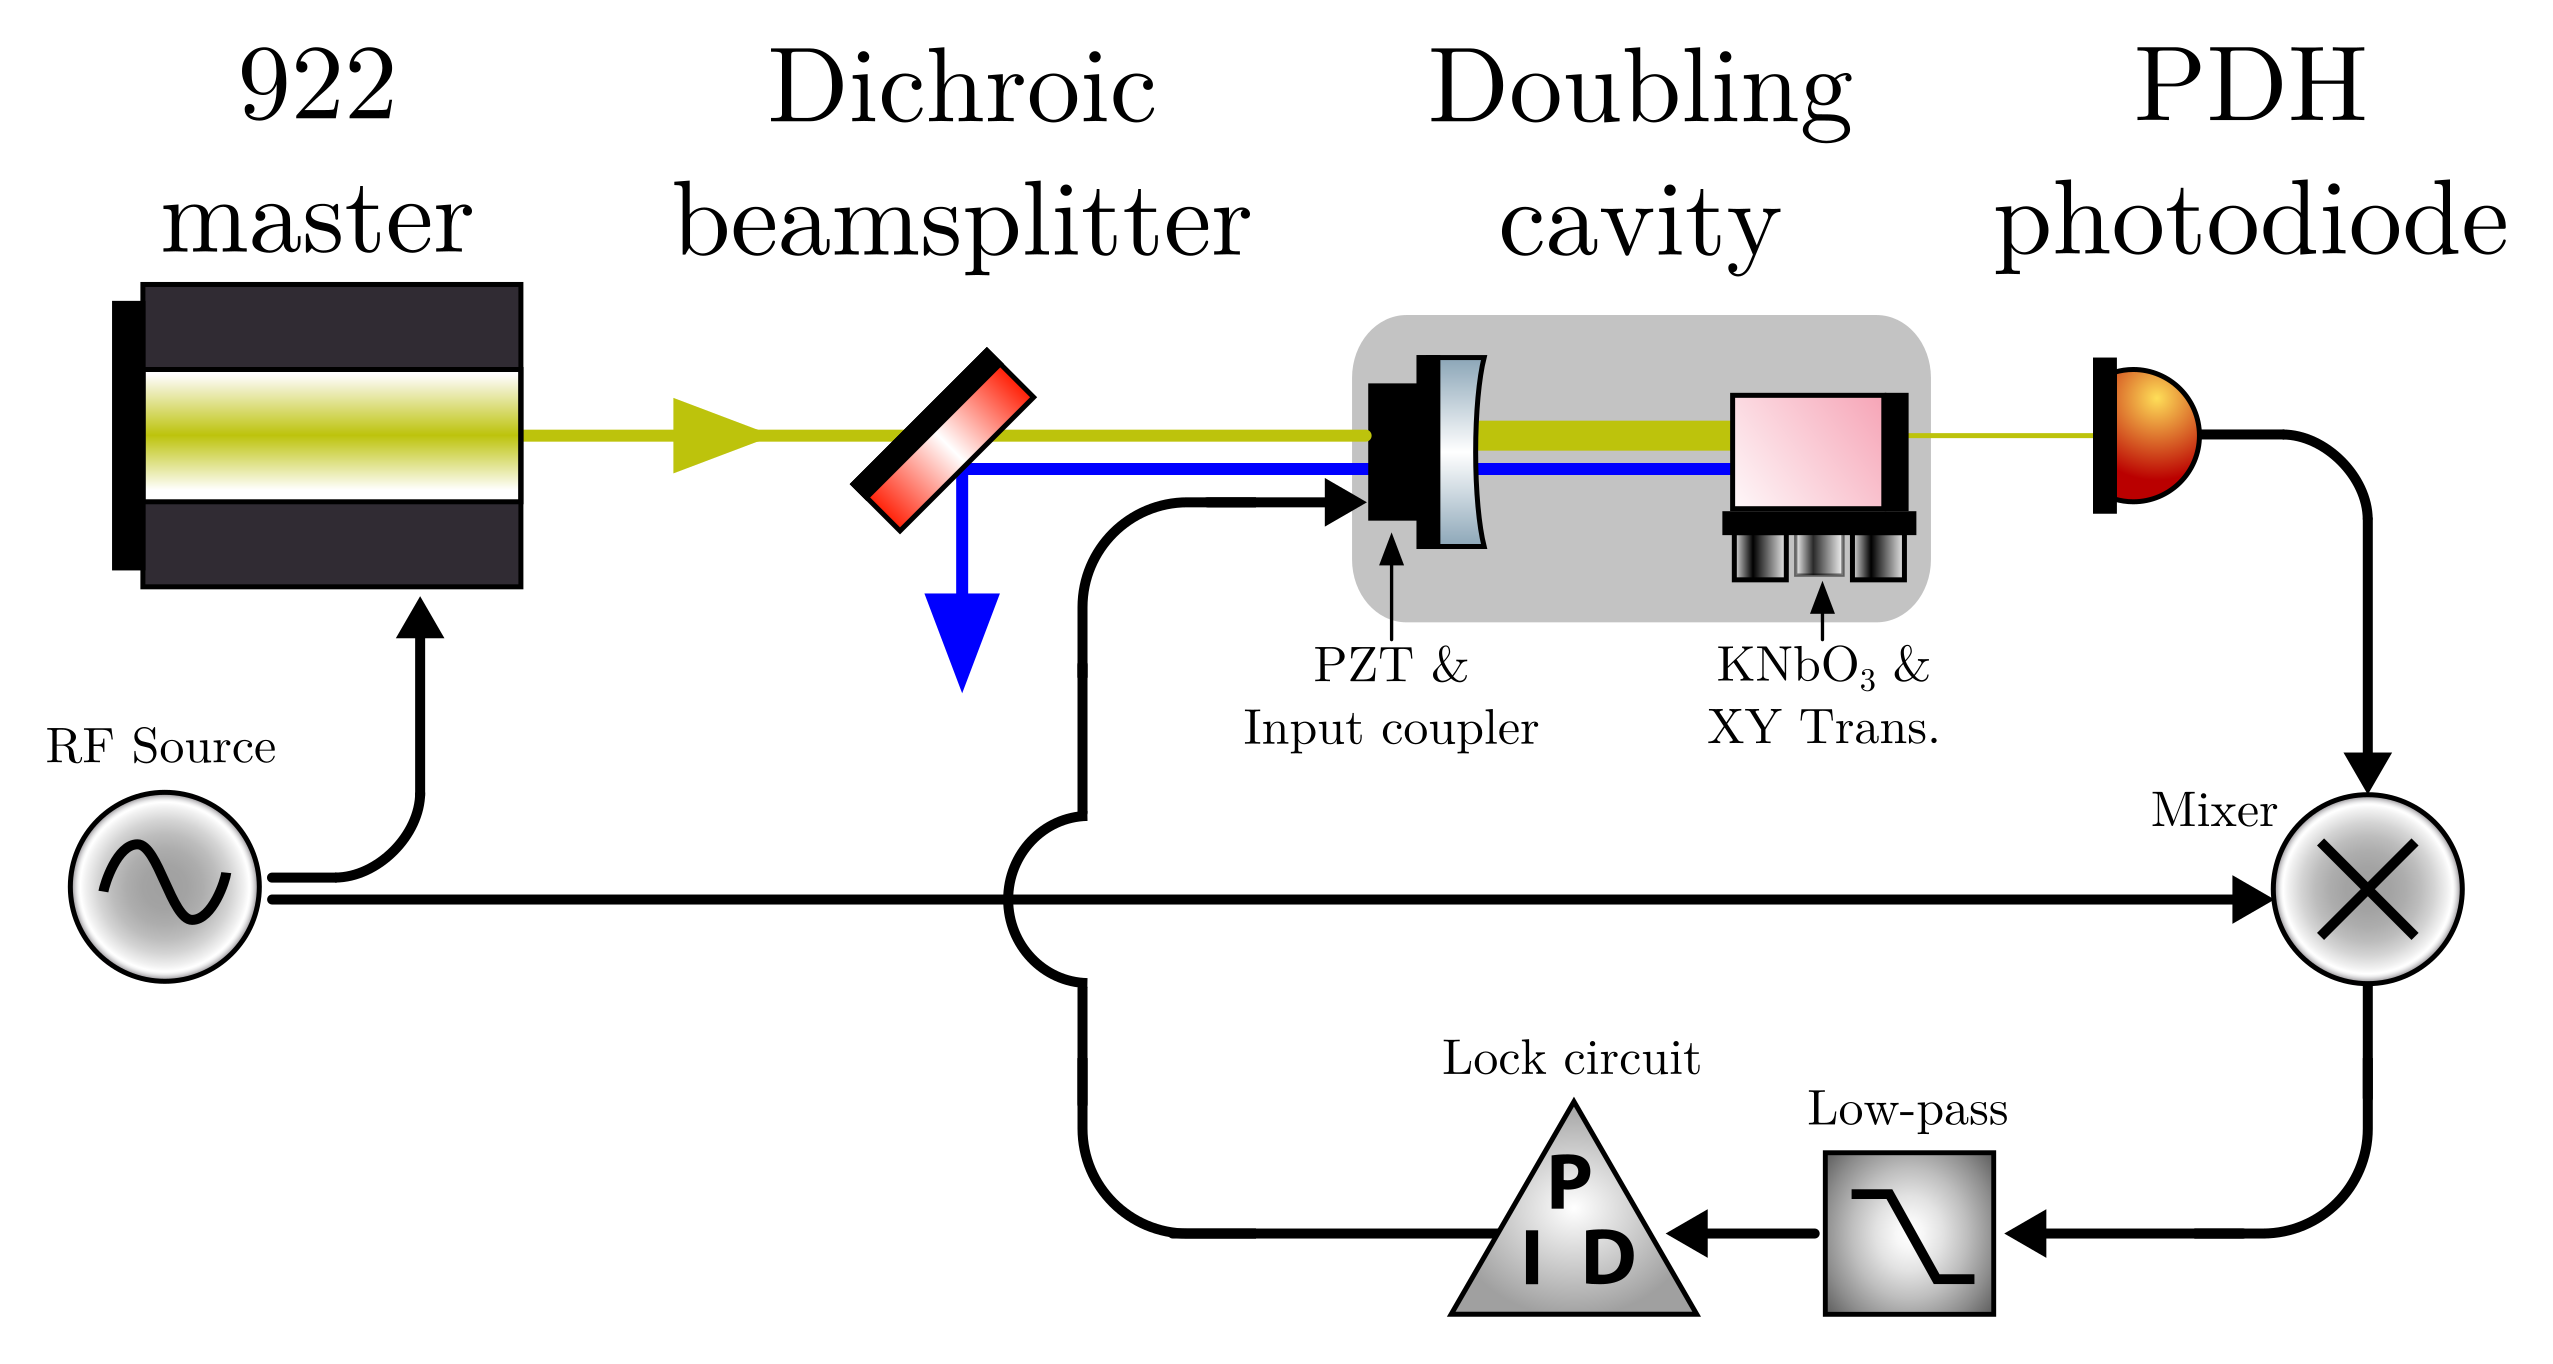
\includegraphics[width=\textwidth]{461cavitystabilization.png}}
		\caption{922\,nm doubling cavity length stabilization feedback diagram}
		\label{fig:461cavityLock}
	\end{figure}
Light out of the 922 master has sidebands added via a high bandwidth AC coupled current modulation directly to the laser diode 
\footnote{This direct coupling means the RF must be turned on prior to enabling the DC current. 
Conversely, the DC current should be disabled before turning off the RF source. 
Failure to follow this order may result in destruction of the laser diode.}.
The doubling cavities of the MOT and Zeeman sub-systems are length stabilized via these sidebands using the Pound-Drever-Hall (PDH) technique \hl{refs}.
Currently, the reference oscillator RF source is a PTS 160 from Programmed Test Sources with an output power of 12 dbm and frequency of 39.55 MHz.
This RF is sent to a 3-way power splitter (model: Mini Circuits ZSC-3-1) which sends roughly a third of the power ($\sim$ 4 dbm) to each of the MOT and Zeeman PDH mixers for demodulation. 
The remaining third is attentuated by 3db before coupling directly to the laser diode.

Once 461\,nm light is available, we stabilize the frequency of the 922\,nm using light from the MOT sub-system to interrogate a strontium heat pipe via frequency modulated Doppler-free saturated absorption from which an error signal of the $^1S_0\,\rightarrow\,^1P_1$ transition is derived.
As shown in Fig.\,\ref{fig:922freqLock}, this error signal is sent into a homemade integrator circuit with a fast feedback path controlling the 922\,nm diode current and a super low-bandwidth\footnote{This super low-bandwidth lock is based on an Arduino PID controller with a low time constant and was built by Josh Hill.
We refer the interested reader to Josh's forthcoming thesis for details of this general purpose slow lock.} 
path controlling for long term frequency drifts via the ECDL's internal PZT.
	\begin{figure}
		\centerline{
		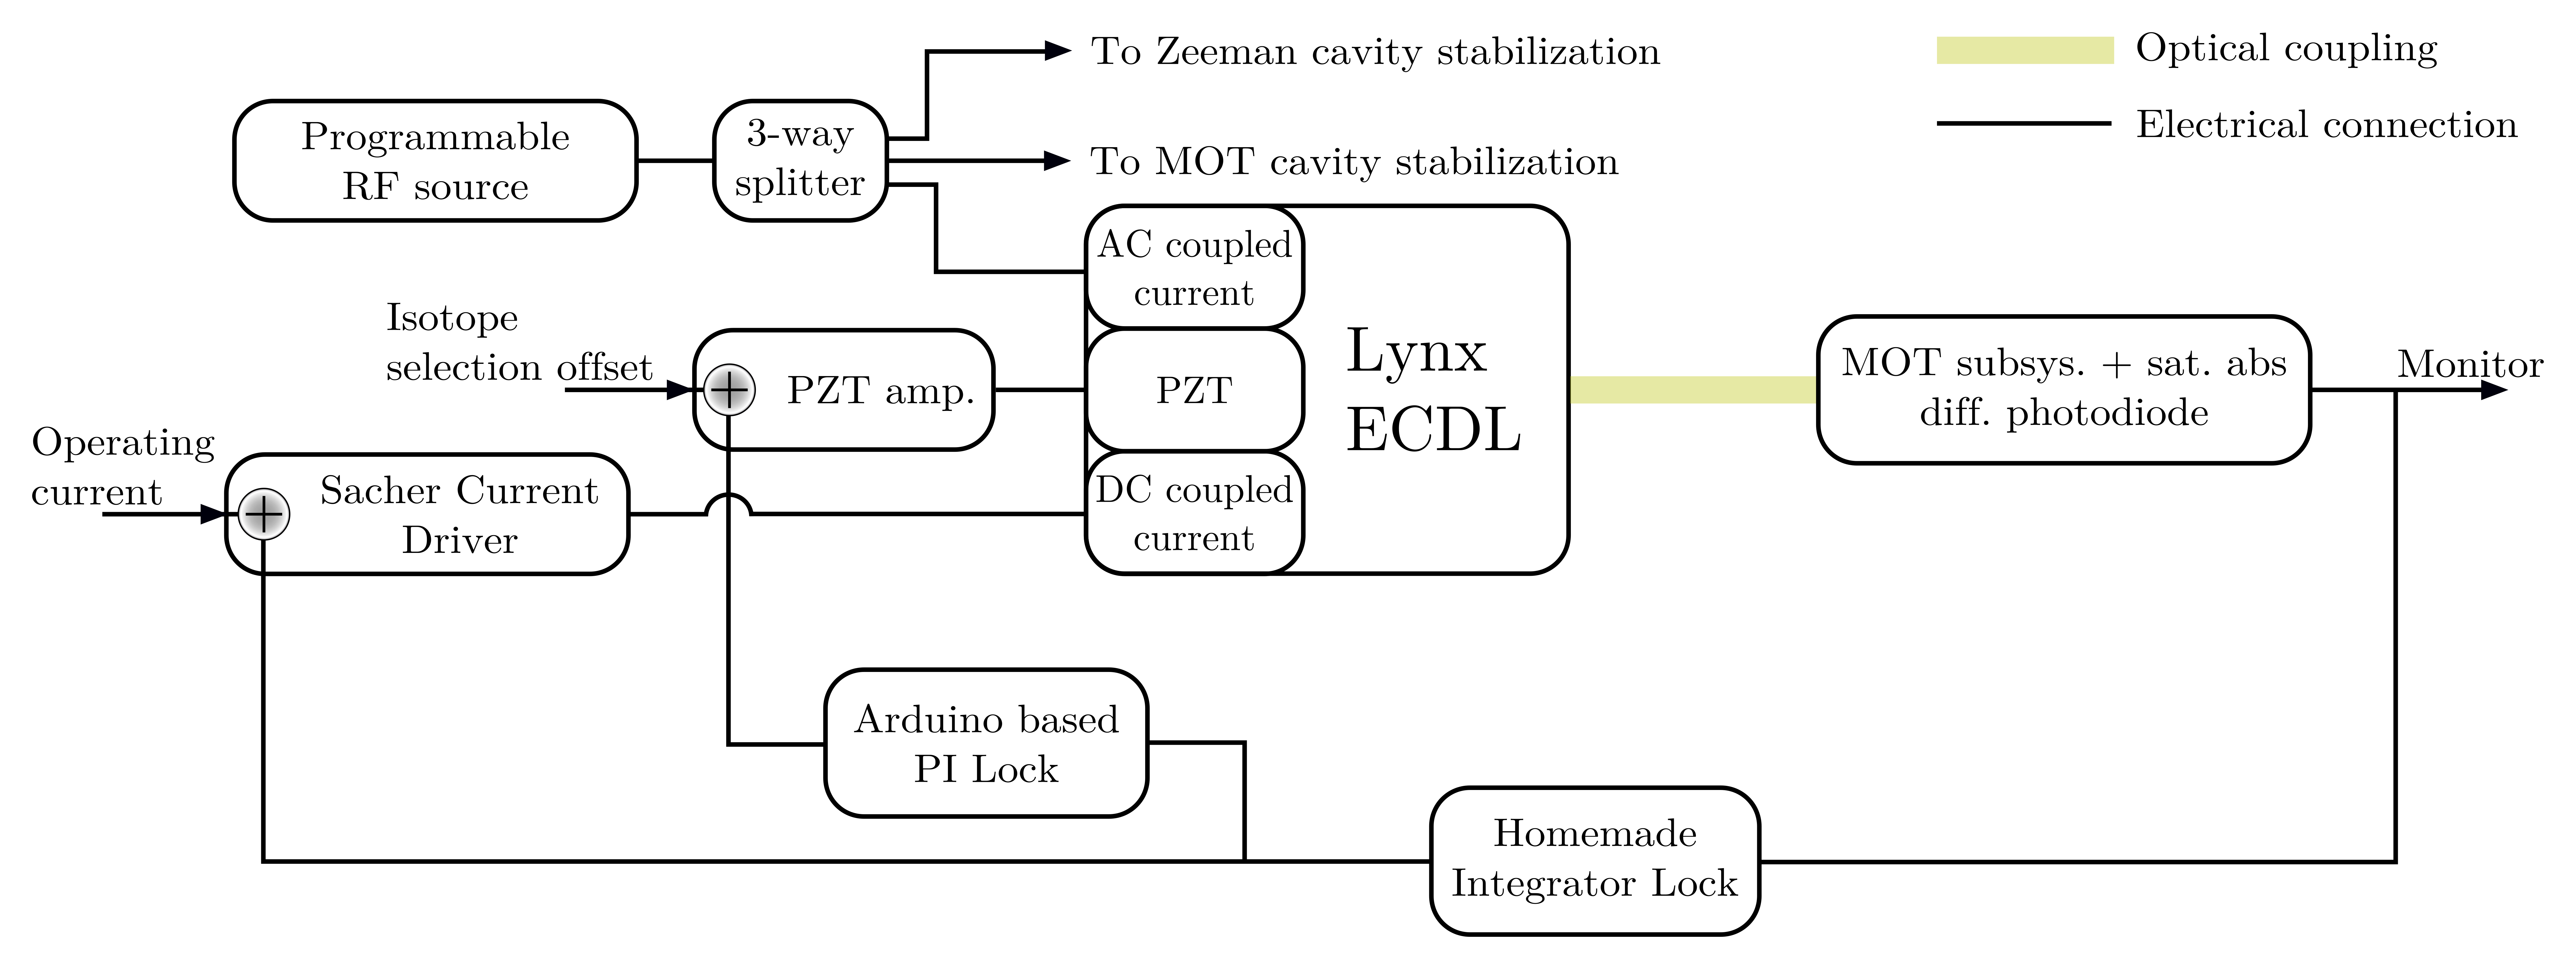
\includegraphics[width=\textwidth]{461_922feedback.png}}
		\caption{922\,nm frequency stabilization block diagram}{Multiple feedback paths allow for controlling the 922 master across disparate timescales. Note that the generation of the error signal used in the feedback is optically connected to the 922 master via the MOT subsystem and sat. abs. setup discussed in Sec.\,\ref{sec:motsubsystem}.}
		\label{fig:922freqLock}
	\end{figure} 
We found that addition of this super low-bandwidth lock has significantly improved the continuous lock time of the 461 system. 
When enabled, the experiment may stay locked for upwards of 24 hours at a time. 
As expected, such an increase in stability has greatly improved our ability to take data over long periods.
Additional details on the original construction of the 922\,nm system can be found in App. A.8 of Natali's thesis \cite{MartinezdeEscolar2010}.

\paragraph{Historical notes and tips for usage}
\subparagraph{PZT driver and replacement:}
The PZT driver provided by Sacher has become problematic over the laser few years.
When varying the voltage we would occasionally hear a "clicking" noise from the Lynx laser as if the voltage was abruptly changing.
We moved to a Thorlabs analog PZT driver (model: MDT694A) and have not had this issue since the switch.
Note that the maximum voltage for the Sacher PZT is 100 V so the driver should be limited accordingly.
Additionally, we attempted to use the newer Thorlabs MDT694B which incorporates an enable control on the voltage knob via a digital potentiometer instead of the analog pot of the "A" model.
However, we quickly abandoned the "B" model as the resolution of the digitization caused the laser frequency to jump large amounts and we were unable to maintain the frequency lock.

In early 2017, we found that the Lynx PZT was no longer responding to applied voltage.
We believe this was caused by the afore mentioned "clicking" issue and was the motivation for changing PZT drivers.
Details and pictures of the PZT replacement are available in App. \hl{something}.

\subparagraph{Sacher temperature setpoint:}
Unfortunately, the woes of the Sacher equipment have not been limited to their PZT controller.
Great care must be taken when attempting to change the set temperature of the laser diode as it seems that the internal potentiometer does not maintain full contact such that when attempting to turn it ever so slightly the set point temperature may jump from approx 16 \degreeC to 11 \degreeC.
Worse yet, we have observed that after changing the temperature there is a settling time during which the temperature setpoint may change while not be monitored.
For these reasons we generally avoid touching this control as the present setpoint of 16.1 \degreeC is adequate and no major improvements have been found when changing this temperature.

\subparagraph{Daily alignment:}
The input coupler for the 922 cleanup fiber is not a reliable mount and tends to drift significantly from day-to-day.
Therefore, we find it useful to peak up the alignment into this fiber while monitoring the output power at a fixed position after the fiber.
Importantly, the positioning of the power meter head seems to effect the amount of power measured by the device (especially as the head ages).
Thus, we use optical mounts in an attempt to reproduce the spatial position everyday and typically acheive a coupling efficeincy of $\sim$51\% through the fiber.
See Sec. \ref{sec:dailyStats} for more details.
		
\subsubsection{Zeeman subsystem}
The Zeeman sub-system is a dedicated TA + doubling cavity for generating approx. 125 mW of 461\,nm light exclusively used for the one-dimensional Zeeman cooling stage.
%There are numerous works exploring the construction and optimization of Zeeman coolers for use with strontium \hl{genetic ref, francy ref, others?}.
This system was originally constructed by Aaron Saenz \cite{AaronDSaenz2005} with additional details available in App A.8 of Natali's thesis \cite{MartinezdeEscolar2010}.
Figure \hl{something} shows a simplified optical schematic of this system.
	\begin{figure} 
		\centerline{
		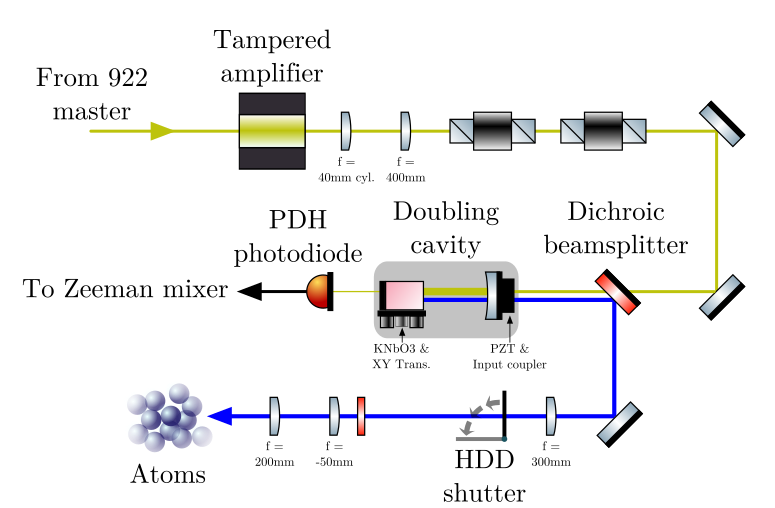
\includegraphics[height=0.4\textheight]{461_zeemanSubsystem.png}}
		\caption{Zeeman subsystem optical schematic}
		\label{fig:zeemanSchematic}
	\end{figure}
Light from the 922 master (approx. 20 mW) is shaped and coupled into a tapered amplifier to produce nearly 300 mW of 922\,nm light.
After being shaped further and passed through dual isolators, the light is then coupled into the homemade doubling cavity where a potassium niobate crystal is held within an optical resonance cavity to produce the 461\,nm light.
For approx. 300 mW into the cavity we are able to produce approx. 125 mW of 461\,nm light.
This light is sent through a final beam expander and into the chamber where we have designed the system to focus the Zeeman beam just at the tip of the atom nozzle to maximize the spatial and temporal interaction between hot atoms and the Zeeman beam.
Table \hl{something} provides typical running characteristics of the system \hl{note thermistor in table}

\paragraph{Historical notes and tips for usage}
\subparagraph{Mode hop:} 
Doubling cavities at such short wavelengths are known to be mercurial \hl{aaron refs} so stabilizing them can be difficult. 
We find that this cavity tends to become stable with \hl{whatever the input power is} as increases of the input power beyond this result in an initial cavity lock producing more 461\,nm light but which quickly mode hops into a lower power mode.
While we have seen cavity output powers of up to 150+ mW, these are not stable modes.
Additionally, the locking circuit contains an auto re-lock feature that can occasionally result in locking to a lower power mode, usually around $\sim$80 mW.
We have found that power cycling the TA current driver is the least intrusive and typically successful method to reattain the 125 mW output.
If cycling does not work, then the TA current output may need to be adjusted.

%\subparagraph{Beam quality:}
%Great care has been taken to minimize any structure present on the 461\,nm Zeeman beam in order to maximize the amount of stopping force which can be derived from this beam.
%Fig. \ref{fig:461zeemanBeam} shows the Zeeman beam just before entering the chamber.
%The cause of the intensity asymmetry which can be seen to the right is unknown, but has been confirmed to be present even directly out of the doubling cavity.
%	\begin{figure}
%		\centerline{
%		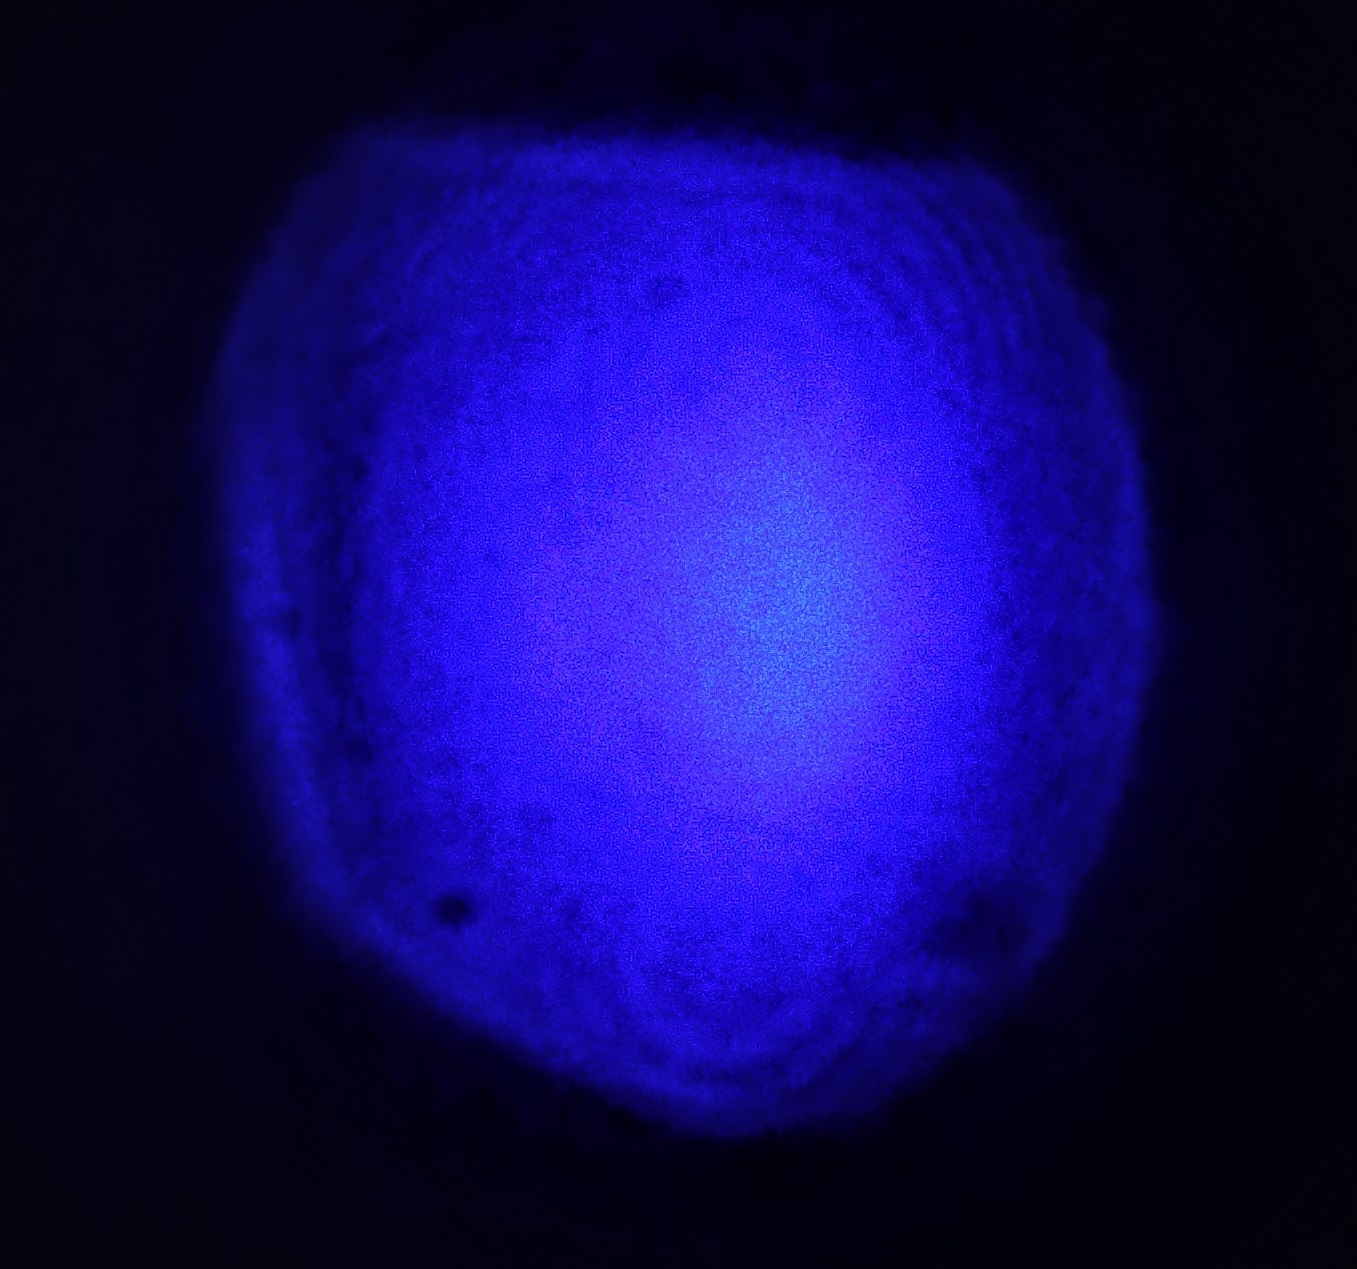
\includegraphics[height=0.25\textheight]{461_IMG_20171213_13048.jpg}}
%		\caption{Characteristic beam quality of the Zeeman laser}
%		\label{fig:461zeemanBeam}
%	\end{figure}
%	
%	Zeeman TA
%		Components
%			Mounts
%			Optics
%			Circuits
%				current control board
%				temp control board
%					note the thermistor in use
%		Typical running values
%			in power
%			out power
%			TA current
%			TA temp
%		
%	Cavity
%		Components
%			Optics
%		Typical running
		
\subsubsection{MOT subsystem} \label{sec:motsubsystem}
The MOT path generates light used for a multitude of processes as shown in Fig \ref{fig:461blockSys}.
Here we detail the systems required for laser cooling and trapping, leaving the details of the blow away pulser and absorption imaging to be discussed in Sec. \ref{ssec:op_tools}.
Furthermore, we begin our discussion wih a focus on the light generation of the MOT subsystem and next we will explore the child setups derived from this subsystem.

Fig.\,\ref{fig:motSchematic} shows a simplified optical schematic of the MOT subsystem which is modeled after the Zeeman setup described previously.
Light from the 922\,nm is shaped, amplified, and coupled into the doubling cavity where the same feedback mechanism shown in Fig.\,\ref{fig:922cavityLock} is used to stabilize the cavity length.
	\begin{figure} 
		\centerline{
		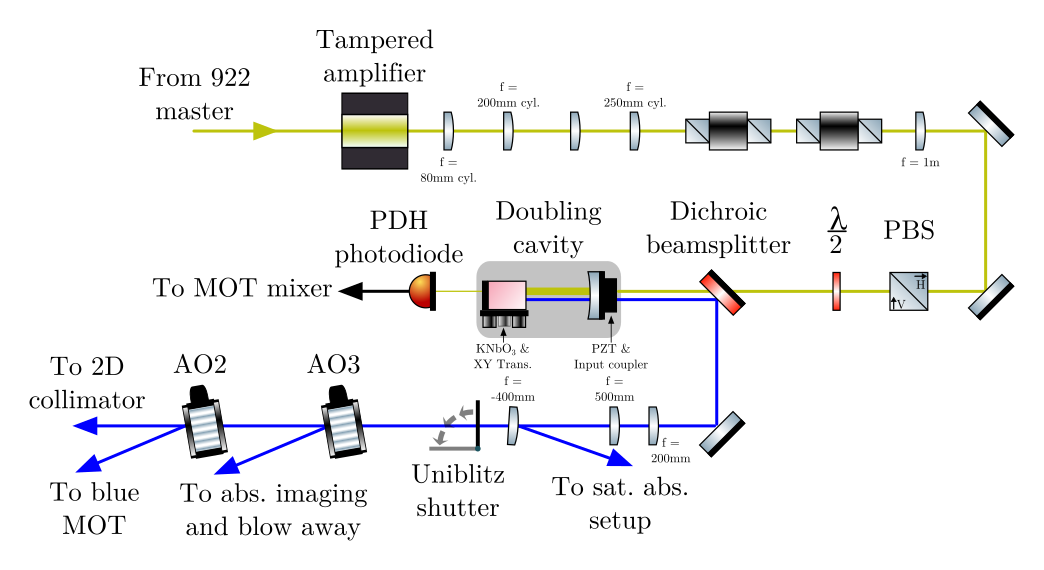
\includegraphics[width=\textwidth]{461_motSubsystem.png}}
		\caption{MOT subsystem optical schematic}{Note the sharing of power between the 2D collimator and blue MOT paths. While the blue MOT is power stabilized as shown in Fig.\,\ref{fig:blueMOTSchematic} the 2D collimator utilizes the remaining laser power.}
		\label{fig:motSchematic}
	\end{figure}
Since the MOT system is situated close to the experimental chamber, a "black-house" wall and shroud were constructed to minimize stray reflections.
This enclosure was placed around the MOT subsystem to mitigate stray 461\,nm light which can significantly hinder the achievement of quantum degenerate strontium gases.
\footnote{Even stray reflected light off the glossy ceiling of the experimental enclosure has been found to cause atom heating!}
Part of this enclosure is a fast ($\sim$2 ms) shutter (model: Uniblitz CS45) used to block the 461\,nm light during the red MOT and evaporation stages.
Additional hard drive (HDD) shutters are also placed along the MOT path behind the black-house shutter as leakage light through the blue MOT AOM (AO2) specifically was seen to cause additional heating when utilizing the blow away pulser.

One concern we face with this MOT setup is the coupling of power between the various paths.
Typically we do not operate the imaging \& blow away pulser while trapping so all available power from the doubling cavity is available for these processes.
However, the 2D collimator and 461\,nm MOT operate concurrently during the first stages of trapping so the available laser power must be split between these two systems and thus an equilibrium must be found which balances the optimum trapping force and the optical molasses of the collimator.
We have observed the 2D collimator to increase the number of trapped atoms in the 461\,nm MOT by about a 7x factor when operating optimally.

\paragraph{461\,nm MOT}
Fig.\,\ref{fig:blueMOTSchematic} gives an overview of the 461\,nm MOT optics\footnote{The MOT arms are labeled as they are organized on the table, where Arm B is closest to the "computer side" of the table.}.
Separation of the laser beams is performed on the table level where custom dichroics are used to combine the 461 and 689 MOT paths.
Following the dichroics, the MOT beams are directed up to the platofrm layer via periscopes and subsequently pass through dual wavelength waveplates which retard 461\,nm light by three-quarters of a period and 689\,nm by one-quarter.
This setup allows us to maintain well defined polarization along the MOT paths.
	\begin{figure} 
		\centerline{
		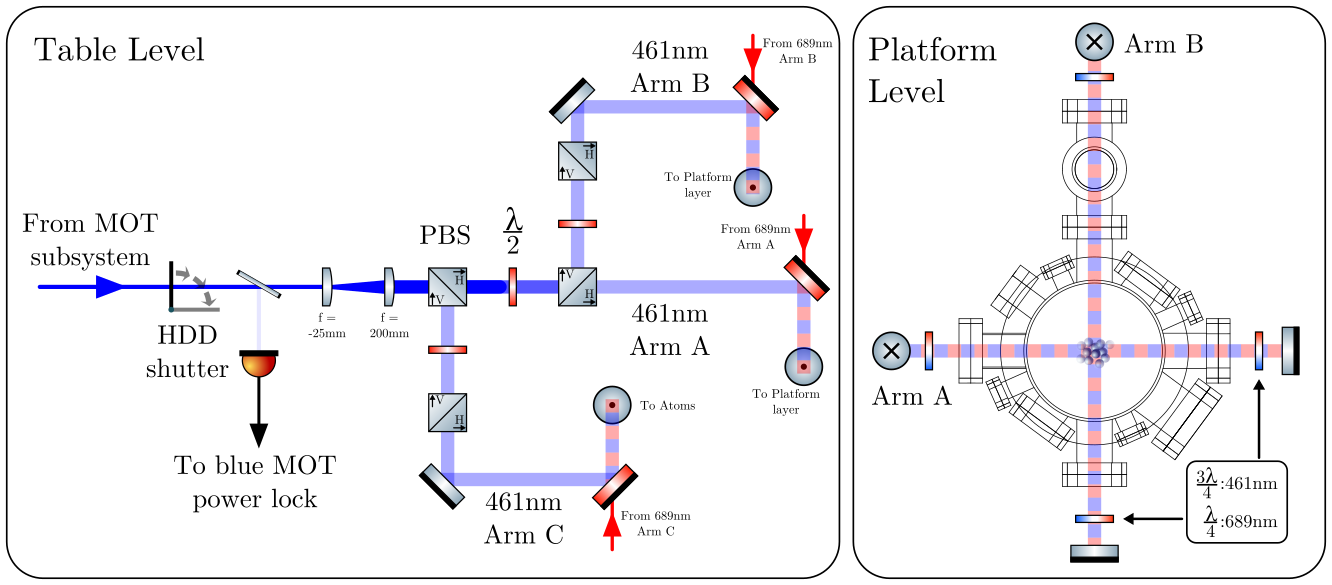
\includegraphics[height=0.4\textheight]{461_blueMOTschematic.png}}
		\caption{461\,nm MOT schematic}{Typical MOT setup with an additional HDD shutter to mitigate light leakage from AO2. Transparency of the laser beams represents the intensity. Note the 461\,nm and 689\,nm light follow the same path through the science chamber. Custom waveplates acting on both wavelengths are used to provide the appropriate polarization.}
		\label{fig:blueMOTSchematic}
	\end{figure}
Each MOT beam operates with $\sim$\hl{num}\,mW of power with a beam size $\sim 1$\,in. for a trapping intensity \hl{??}.
During MOT operation this intensity is locked via an intensity stabilization circuit.

%Characteristic power in each beam
%MOT beams are power controlled via the feedback system shown in fig.
%The custom power lock integrated circuit is given in \hl{figure in appendix}.
%This design is based off the work report by Ying Huang but with several modifcations for adding a transimpedence amplifier as the input stage.
%The power setpoint is a controlled input from the 	

\paragraph{Saturated absorption}
The saturated absorption cell is used to interrogate the $^1S_0\,\rightarrow\,^1P_1$ transition in order to lock the frequency of the 922 master.
App. \ref{app:dopSpec} outlines a brief derivation for determining the lock point when a constant offset is added to the laser frequency, as is the case here.
As outlined in the derivation, by utilizing the Zeeman tunability of magnetic sublevels, we can shift the resonance frequency of the atoms in the heat pipe.
Thus, by interrogating and locking to the transition frequency of the most abundant isotope, $^{88}$Sr, we can shift it's resonance to cover the isotope shifts of the other strontium isotopes.
This provides a simple method for trapping various isotopes and mixtures of strontium.

A detailed walkthrough of the construction and relevant physics of a blue sat. abs. cell can be found in the undergraduate report of Michael Viray \cite{MichaelViray2014}.
Additionally, the original construction of the Neutral cell is covered in section 2.2.1 of Natali's thesis.
Fig.\,\ref{fig:blueSatAbs} shows the optical setup used to generate the error signal and reference traces of Doppler bowl and frequency lock error signal.
This error signal is generated by frequency modulating the magnetic field of the cell and performing Doppler free saturated absorption.
	\begin{figure} 
		\centerline{
		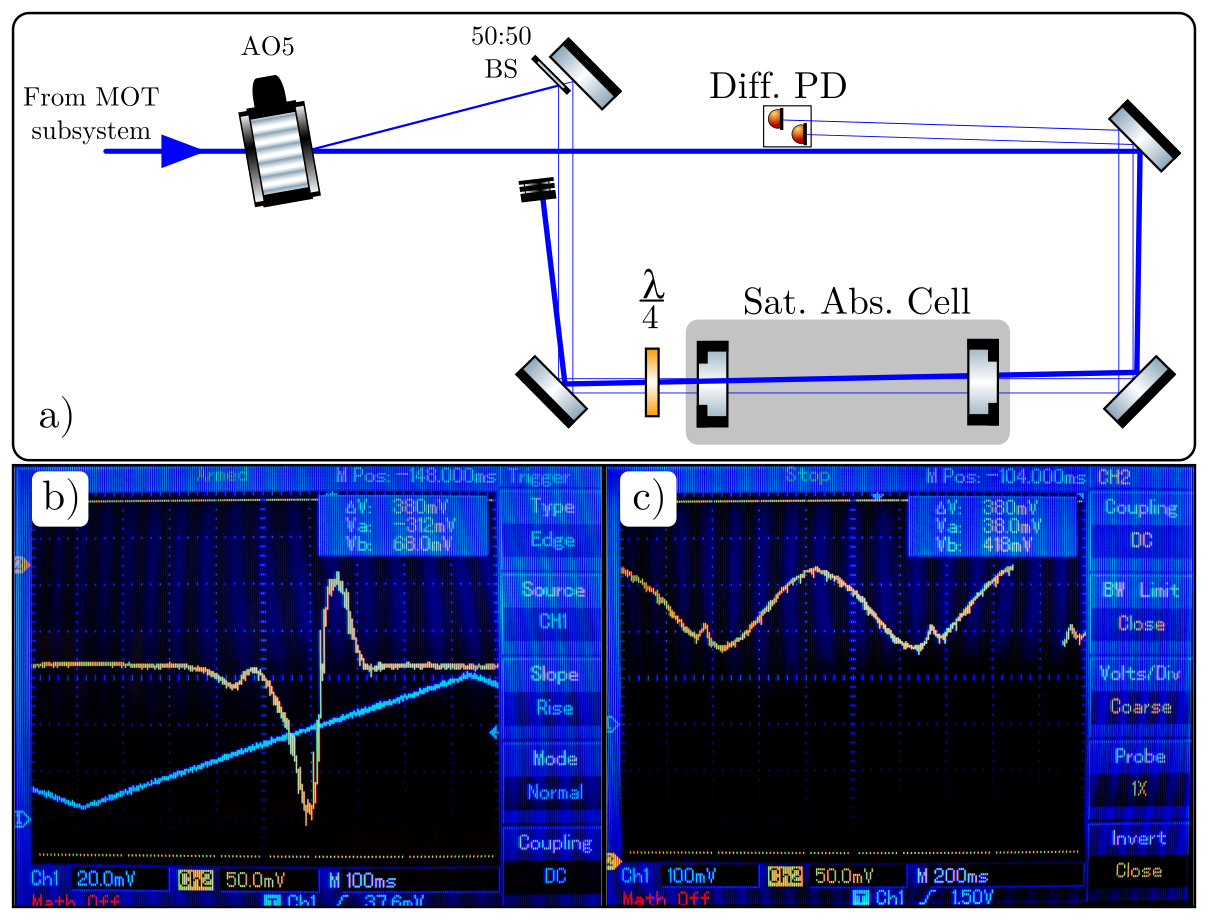
\includegraphics[width=0.7\textwidth]{461_satAbsSchematic.png}}
		\caption{461\,nm saturated absorption setup}{a) Optical setup for frequency locking the 922\,nm master. b) Example error signal. The cause of the asymmetry is unknown but occurs around approx. $\pm$1.7A drive. The offset seen here can be nulled by balancing the amplification applied to the differential photodiode inputs. c) Example of the Doppler bowl where the Lamb dip can be seen. Note that the Lamb dip interacts with a specific velocity class determined by $\delta_{SA}$.}
		\label{fig:blueSatAbs}
	\end{figure}

\paragraph{Historical notes and tips for usage}
\subparagraph{Daily alignment of MOT TA:}
The simplified optical schematic of the MOT subssytem in Fig.\,\ref{fig:motSchematic}, does not reflect the approx. two meter lever arm which is present between the Zeeman split AOM and the input to the MOT TA due to the relative positions of the cavities.
We have found this requires us to peak up the alignment of the 922 master beam into the MOT TA on a daily basis and is hypothesized to be the cause of large long time power variations ($\sim$15\%) on the output power of the MOT cavity which we observe throughout the course of the day.
Typically with an input power of approx. 300 mW of 922\,nm light we get between 100 - 115 mW out on a daily basis.

\subparagraph{Note on changing isotopes:} \label{para:change_iso}
While the basic setup has not changed over the many years, we have recently moved away from the original current source based on a home built high-current FET amplifier to a Bi-polar current source (BOP) (model: Kepco BOP-20-10DL).
This change allows for more expansive coverage of the $^1S_0\,\rightarrow\,^1P_1$ isotopes shifts. The previous current source limited our dual trapping capability to 87+88, and required an AOM to be tweaked and the sat. abs. to be realigned for trapping 84 and 86. 
Using the BOP, we can now easily shift the transition frequency over approx. $\sim$200 MHz which allows us to span the range between 84 and 87 within a single experimental cycle.
Given the geometry of our solenoid, large currents are required to apply such large Zeeman shifts.
We have observed that these large currents increase the heat load on the cell, which can lead to a reduction in the error signal.
We mitigate this additional heating by varying the heater current to maintain approx. 50\% absorption of the pump beam.
As we expect, the timescale for these effects are minutes, so short term variations (i.e. when doing spectroscopy) do not cause significant heating when the duty cycle is kept low.

Due to the heating from the Zeeman coil, we chose to balance the currents needed to trap 84 and 87 by "centering" the pump-probe beams frequency such that the magnitude of the currents needed for both isotopes is similar, but with 84 requiring a $(+)$ current and 87 a $(-)$ current.
However, trapping of 88 still requires the realignment of the sat. abs. pump-probe beams as this shift is just beyond the capabilities of the current drive. 
Care should be taken when adjusting this alignment as the paths are highly coupled as can be seen in Fig.\,\ref{fig:blueSatAbs}a).

%Simplifed optical schematic
%
%While realigning the sat. abs. is not always necessary
%
%Give calibration plot?
%
%MOT light path
%	Components
%		TA
%		Cavity
%		AOMs
%		Shutters
%	
%	MOT TA
%		Components
%			Mounts
%			Optics
%			Circuits
%				current control board
%				temp control board
%					note the thermistor in use
%		Typical running values
%			in power
%			out power
%			TA current
%			TA temp
%		
%	Cavity
%		Components
%			Optics
%		Typical running

%\subsection{Repumping: 481\,nm}
%\label{ssec:481sys}
%
%Plot from Rydberg
%
%Discuss the change with the EOM
%	Frequency center of EOM and range?
%	
%Data on picking the timescale?
%	I know I choose like 40ms (including delay, but did I take data on this)
%
%This system is based on a Toptica DL-100 littrow laser which produces about 8mW of power at 481\,nm. 
%Excitation to a doubly excited state is an eay way to do the repumping.
%As it is difficult to create and maintain a population of atoms in the $^3P_2$ state, we use a telerium oven to lock the laser.
%The original setup of this system was done by Pakorn \hl{ref} who setup a side of peak locking scheme. 
%Ten by dithering the laser current we can broaden that laser and extend to the strontium transition.
%
%Recently, we have begun to trap multiple isotopes across the different labs and have found our naive appraoch to locking the repumper to be inadequate.
%Working with the Rydberg apparatus, we performed spectroscopy of the repumping transition by counting the number of atoms which were returned to the ground sate as a function of repumping frequency.
%During these experimens we found that very small amounts of power, on the order of $\mu$W's, is needed to obtain large ground sate populations when the laser is tuned precisely to the isotopic transtion energy. 
%Fig.\,\hl{something} shows the result of this spectroscopy for multiple strontium iotopes.
%It was not feasible to dither the current across the GHz of detuning needed without mode hoping the laser so we decided to use an EOM driven at high power to place multiple orders of sidebands onto the laser light.
%
%What frequency is the EOM running at?
%What frequecnies do we aim to hit precisely?
%
%The current setup uses the EOM in addition to dithering the laser current a small amount to address these transitions.
%With this finding we decided to use an EOM to place multiple orders of sidebands on the laser light
%This allows us to address multiple transitions more precisly
%
%Optical schematic
%Light from this laser is split into five paths.
%One for each experiment, another for monitoring the wavelength, and the last for probing the tellerium transtion.
%
%Feedback diagram
%We have found
%
%\subparagraph{Historical note:}
%The lead screw, which is part of the internal alignment mechanism of the Littrow ECDL, was nearly stripped at some point when attempting to peak up the frequency stability. 
%Extreme care should therefore be taken when using this adjustment as the brass baseplate of the DL-pro is soft and there is a potential to strip out the remaining threads.
%	\begin{figure}
%		\centerline{
%		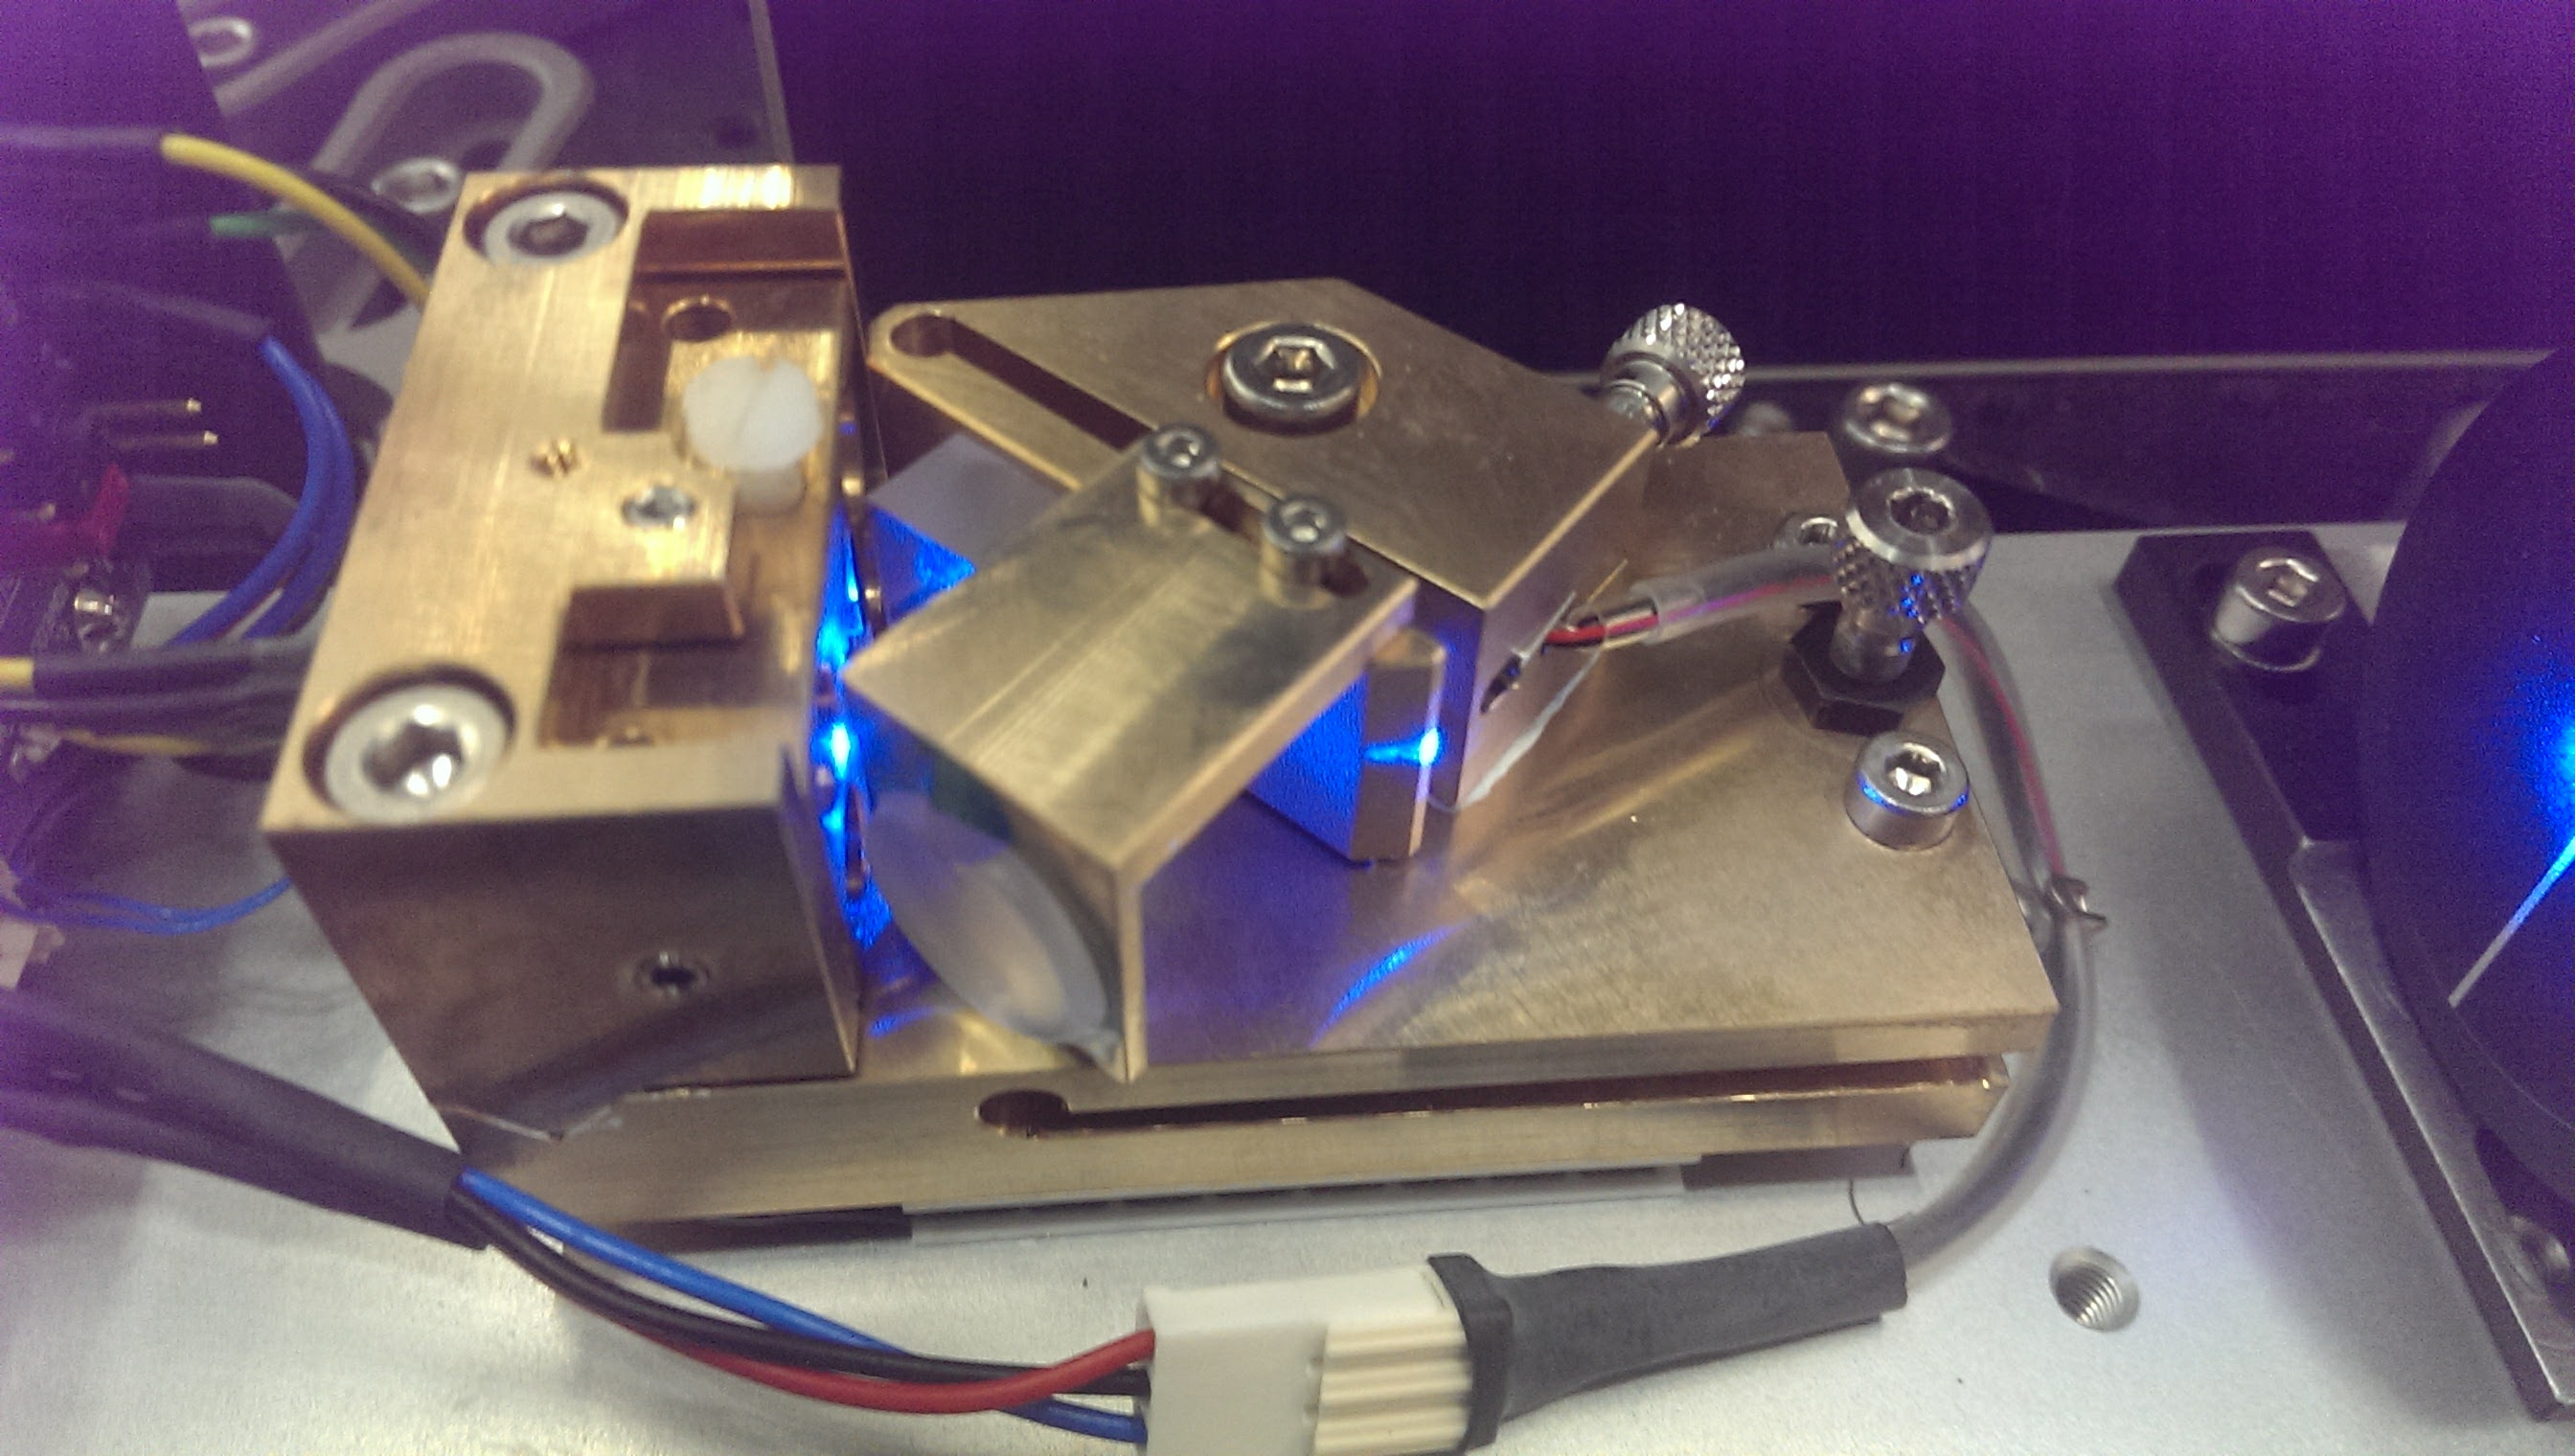
\includegraphics[height=0.2\textheight]{481_IMAG0022.jpg}}
%		\caption{Internal view of the 481\,nm ECDL}{The red box denotes the alignment screw that should be adjusted with caution.}
%		\label{fig:481internal}
%	\end{figure}

\pagebreak
\subsection{Narrowband cooling stage: 689\,nm} \label{ssec:689sys}
\subsubsection{Overview}
The work horse transition of strontium is the $^1S_0\,\rightarrow\,^3P_1$ intercombination line transition at 689\,nm. 
In addition to cooling and trapping, most experiments performed in our lab utilize this transition as our primary probe owing to the narrow linewidth which allows for high precision measurements and large detunings using conventional techniques.

Fig.\,\ref{fig:689blockSys} shows an overview of how we generate and use the 689\,nm light. 
The following section will describe the trapping portions of the red system and Sec.\,\hl{something} will explore the spectroscopy probe setup and it's various configurations.
	\begin{figure}
		\centerline{
		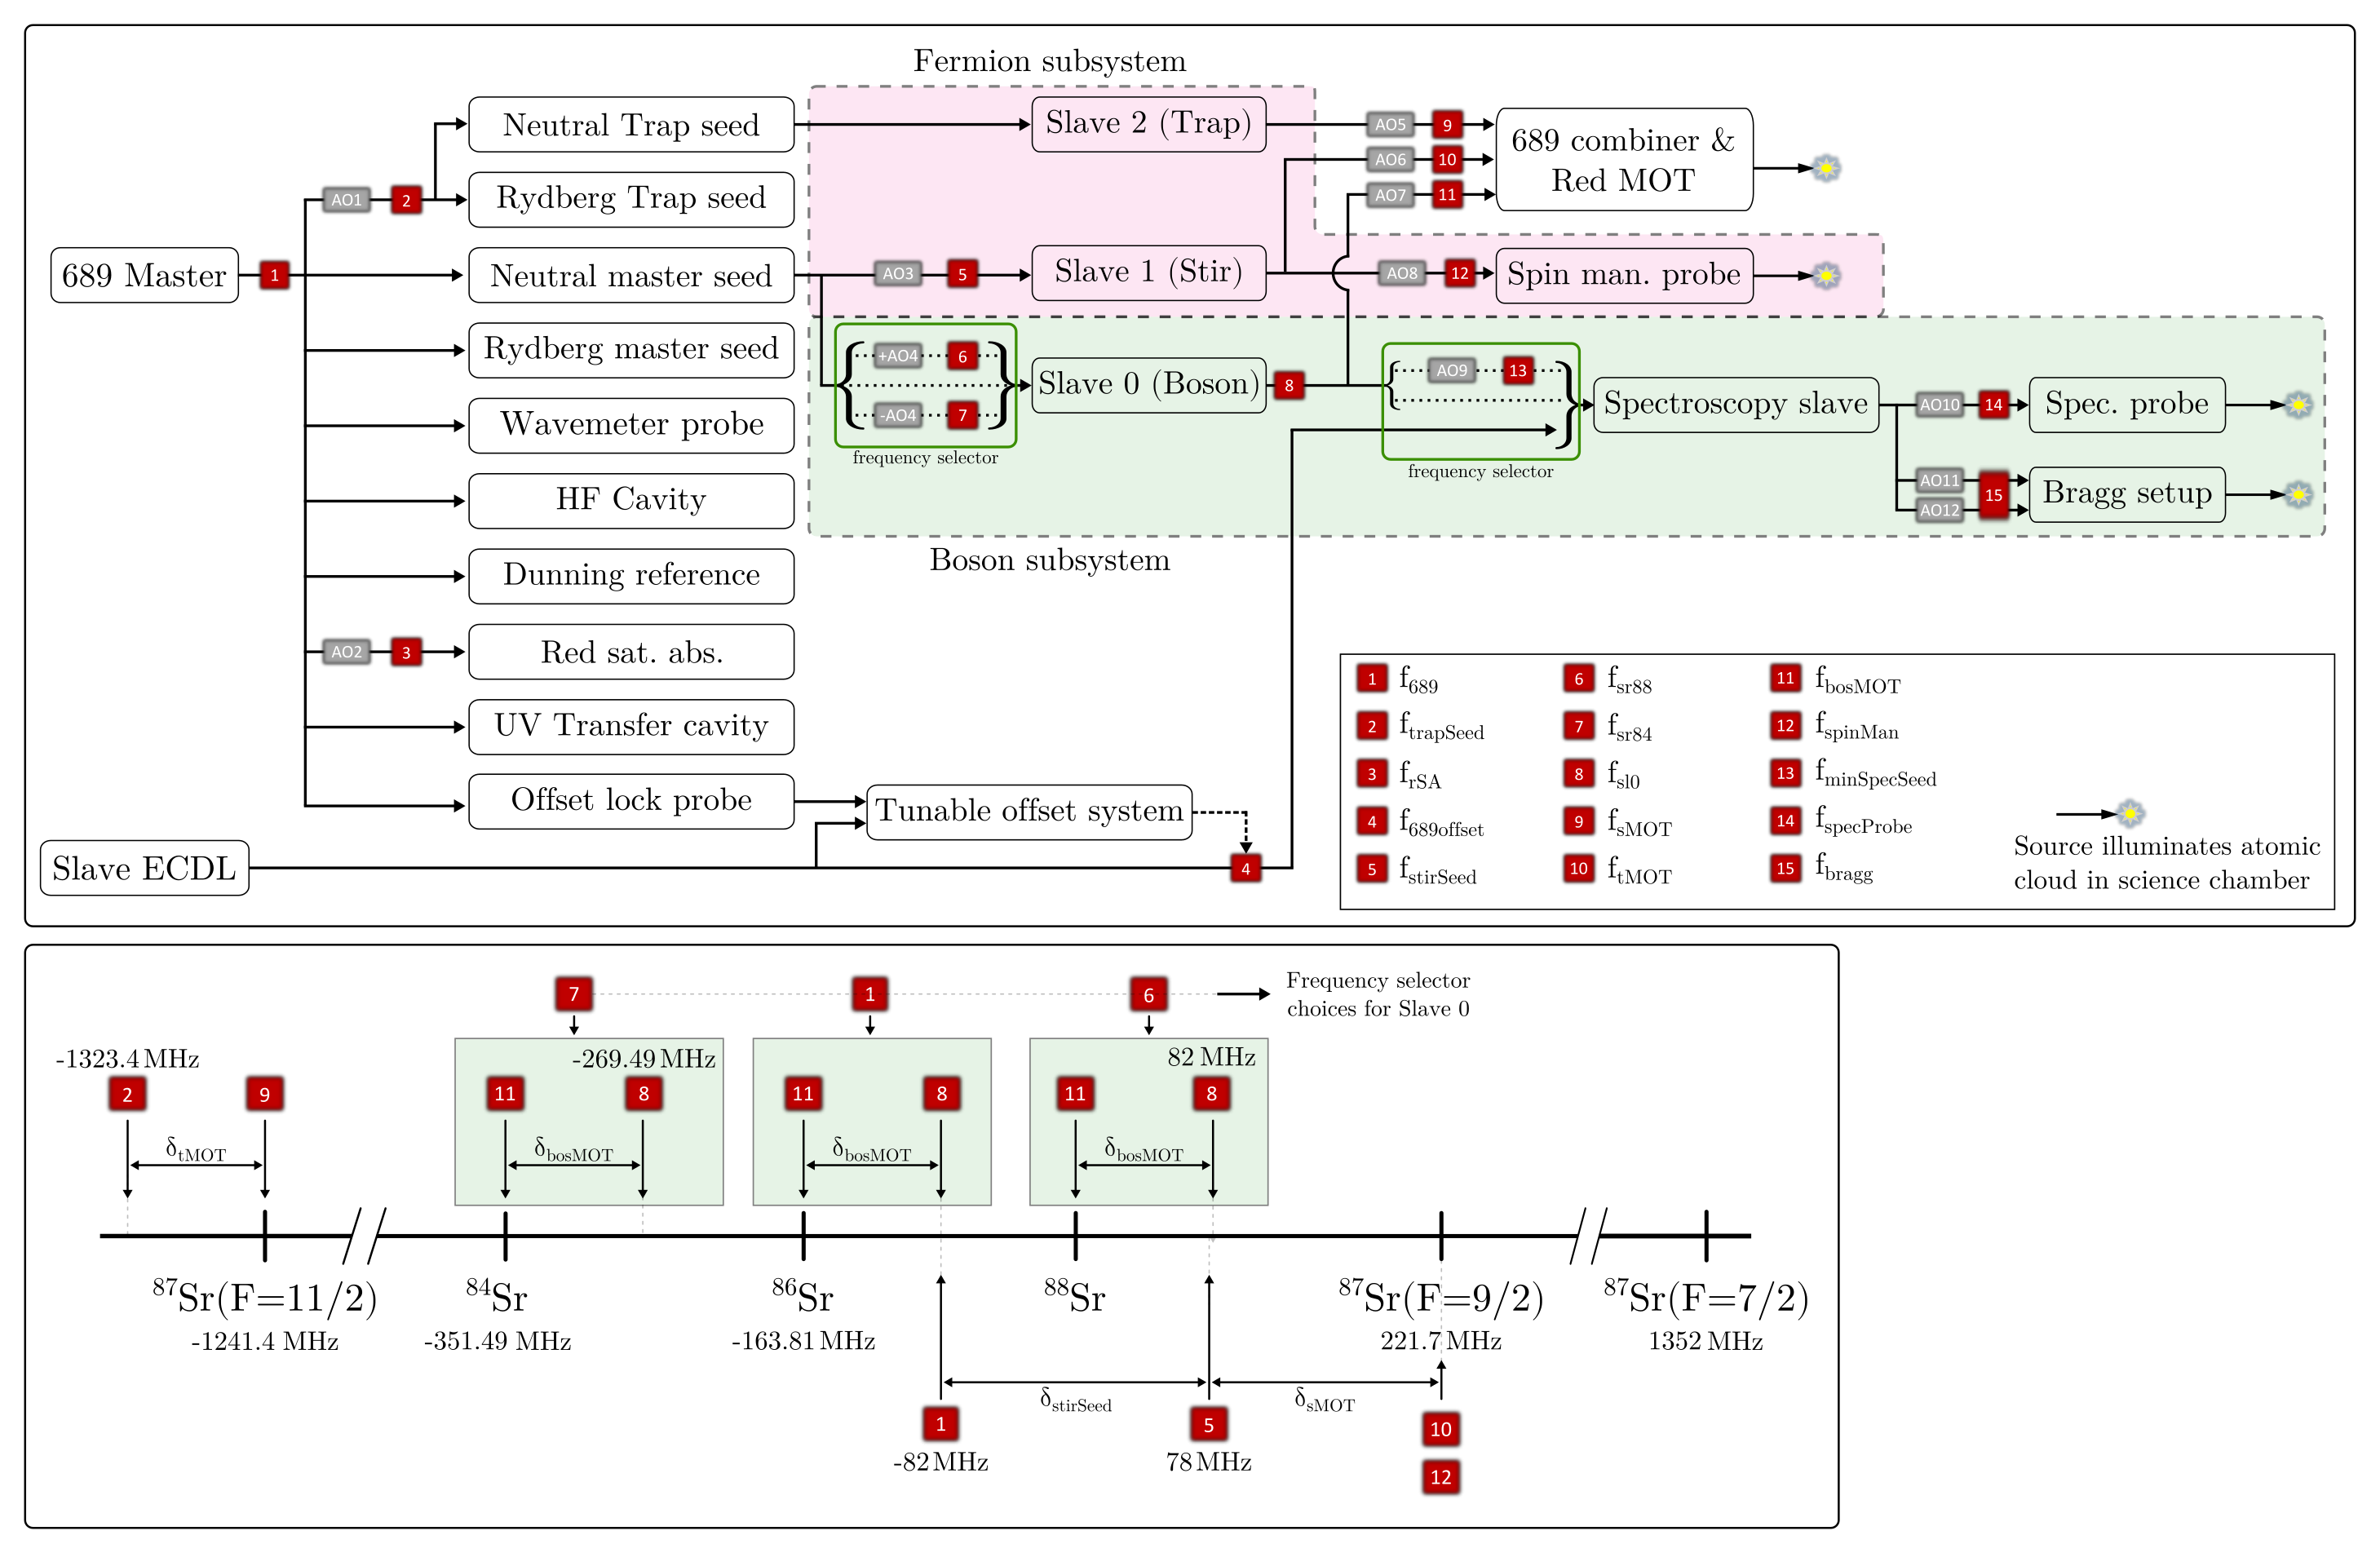
\includegraphics[width=1.3\textwidth,angle=90,origin=c]{689_redSystem.png}}
		\caption{689\,nm light generation system}{Top - Block diagram showing the relations of the various systems, AOMs, and frequencies in use throughout the red system. See Table \ref{tab:689AOM} for information on the AOMs. Bottom - Relevant frequencies for trapping using the Neutral red system.}
		\label{fig:689blockSys}
	\end{figure} 
In conjunction with the block diagram, Table\,\ref{tab:689AOM} details the frequency shifts and AOMs. 
The block diagram denotes the position of these AOMs by the grey squares and the red squares define the various system frequencies determined by the various shifts.
\begin{table}[]
\centerline{
\resizebox{0.8\textwidth}{!}{%
\begin{tabular}{@{}|l|c|c|c|l|l|@{}}
\toprule
\multicolumn{1}{|c|}{\textbf{Label}} & \textbf{Ind.} & \textbf{\begin{tabular}[c]{@{}c@{}}Shift\\ variable\end{tabular}} & \textbf{\begin{tabular}[c]{@{}c@{}}Nominal \\ Freq. {[}MHz{]}\end{tabular}} & \multicolumn{1}{c|}{\textbf{Freq. Source}} & \multicolumn{1}{c|}{\textbf{AOM Model}} \\ \midrule
Trap Seed & AO1 & $\delta_{trapSeed}$ & -1241.44 & Novasource G6 & \begin{tabular}[c]{@{}l@{}}Brimrose\\ TEF-1300-200-550\end{tabular} \\ \midrule
Red Sat. Abs. & AO2 & $\delta_{rSA}$ & +164$\pm$0.5 & \begin{tabular}[c]{@{}l@{}}Novatech 409B\\ (Dithered)\end{tabular} & \begin{tabular}[c]{@{}l@{}}IntraAction \\ ATM-1643DA1\end{tabular} \\ \midrule
Stir Seed & AO3 & $\delta_{stirSeed}$ & +160 & Novatech 409B & \begin{tabular}[c]{@{}l@{}}IntraAction \\ ATM-1602DA1\end{tabular} \\ \midrule
\begin{tabular}[c]{@{}l@{}}Isotope\\ Selector\end{tabular} & AO4 & $\delta_{isoSel}$ & \begin{tabular}[c]{@{}c@{}}+164 or\\ -187.49\end{tabular} & Novatech 409B & \begin{tabular}[c]{@{}l@{}}IntraAction \\ ATM-2001A2\end{tabular} \\ \midrule
Trap MOT & AO5 & $\delta_{tMOT}$ & +82 & \begin{tabular}[c]{@{}l@{}}Trap VCO / \\ Novatech 409B\end{tabular} & \begin{tabular}[c]{@{}l@{}}IntraAction \\ ATM-852DA2\end{tabular} \\ \midrule
Stir MOT & AO6 & $\delta_{sMOT}$ & +143.7 & \begin{tabular}[c]{@{}l@{}}Stir VCO / \\ Novatech 409B\end{tabular} & \begin{tabular}[c]{@{}l@{}}IntraAction\\ ATM-1402DA1\end{tabular} \\ \midrule
Boson MOT & AO7 & $\delta_{bosMOT}$ & -82 & \begin{tabular}[c]{@{}l@{}}Boson VCO / \\ Novatech 409B\end{tabular} & \begin{tabular}[c]{@{}l@{}}Isomet\\ 1205C-2\end{tabular} \\ \midrule
\begin{tabular}[c]{@{}l@{}}Spin man.\\ probe\end{tabular} & AO8 & $\delta_{spinProbe}$ & -144$\pm$2 & Novatech 409B & \begin{tabular}[c]{@{}l@{}}IntraAction\\ ATM-1402DA1\end{tabular} \\ \midrule
\begin{tabular}[c]{@{}l@{}}Spec. slave\\ seed\end{tabular} & AO9 & $\delta_{specSeed}$ & -40 & Novatech 409B & \begin{tabular}[c]{@{}l@{}}IntraAction\\ AOM-402A1\end{tabular} \\ \midrule
Spec. probe & AO10 & $\delta_{specProbe}$ & -82$\pm$20 & Novatech 409B & \begin{tabular}[c]{@{}l@{}}IntraAction\\ ATM-902DA1\end{tabular} \\ \midrule
Bragg \#1 & AO11 & $\delta_{bragg1}$ & \multirow{2}{*}{90$\pm$20} & Novatech 409B & \begin{tabular}[c]{@{}l@{}}Crystal Tech.\\ 3110-125\end{tabular} \\ \cmidrule(r){1-3} \cmidrule(l){5-6} 
Bragg \#2 & AO12 & $\delta_{bragg2}$ &  & Novatech 409B & \begin{tabular}[c]{@{}l@{}}Crystal Tech.\\ 3110-125\end{tabular} \\ \bottomrule
\end{tabular}%
}}
\caption{689\,nm systen AOM details}{Ind. labels the AOMs as shown in Fig.\,\ref{fig:689blockSys}. The sign of the nominal freq. indicates the AOM order.}
\label{tab:689AOM}
\end{table}

All precision frequencies of the 689 system are derived from digital synthesizers with mHz accuracy.
The one exception to this is during the broadband red MOT operation when we use voltage controlled oscillators to effectively broaden the laser linewidth.

The boson and fermion sub-systems allow us to simultaneously trap and cool mixtures of a single bosonic isotope and the fermionic 87.
The isotope selector AOM determines which bosonic isotope this system can trap.
Changing between bosonic isotpes requires the shift from the isotope selector AOM to be changed and light recoupled into the injection lock fiber that is aligned to slave 0.

%Notably, the AC stark shift due to the IR laser is strong enough to require optimization of the red MOT parameters in the presence of the light.
%The optimization is complicated by the influence of gravity on the red MOT which causes the single frequency stage to "sag" which must be overlapped wit the IR light in order to load most efficiently.
	
Recently, the Neutral 689\,nm system has seen significantly growth and been entirely restructured. 
For notes on the original setup refer to App A.3 \& A.4 in Natali's thesis.
The most notable changes have been the replacement of the homemade master ECDL and the move to fiber based injection locks for all slave lasers on the Neutral table.
Furthermore, the master laser system is now shared between the Rydberg and Neutral laboratories and therefore a more modular approach was adopted to ensure independence of the labs experimental schedules. 
This process began with the replacement of our homemade Littman-Metcalf ECDL 689 master with a Toptica DL-Pro system. At the time of this writing (spring 2019) we are currently in the process of migrating from the original high-finesse cavity used for the last 15 years \cite{Nagel2004} of the experiment to an ultra-low expansion cavity system. 

This approach to sharing the 689 light is based on fixing the lock point of the 689 light and fiber coupling this fixed frequency light to the separate experiments. 
From this master fiber we utilize a series of AOMs to choose the correct frequency needed for the experiment at hand. This movement to a fiber based system culminated in the spring of 2018 when the Neutral apparatus significantly refactored our red system and transitioned to an entirely fiber based injection locking scheme. 
Optical fibers provide several key advantages when used to injection lock slaves, namely a much cleaner TEM00 output mode that can be easily mode-matched to the slave. 
Additionally, fibers provide a quick and effective means for ensuring optimal alignment of the injection locking light by coupling the rejected light from the slave diode "backwards" through the fiber. 
Although rejected light is typically minimized when setting up a slave diode, by temporarily placing a waveplate before the isolator you can scramble the input polarization and increase the rejected power to facilitate alignment through the fiber. 
This process generally results in a quite robust alignment of the fiber output and the laser diode and is much faster than the free space method of coupling over a long distance. 
This alignment advantage along with improved mode matching has allowed us to injection lock a slave diode with as little as 300 $\mu$W while producing up to 24 mW of usable output power.

The rest of this section will detail the setup of the 689 system including the master system and both boson and fermion subsystems used for narrowline cooling and trapping.
The primary spectroscopy system and spin polarization setup are outlined in section \hl{ref}.
	
\subsubsection{689\,nm Master}

Optical schematic
	\begin{figure} 
		\centerline{
		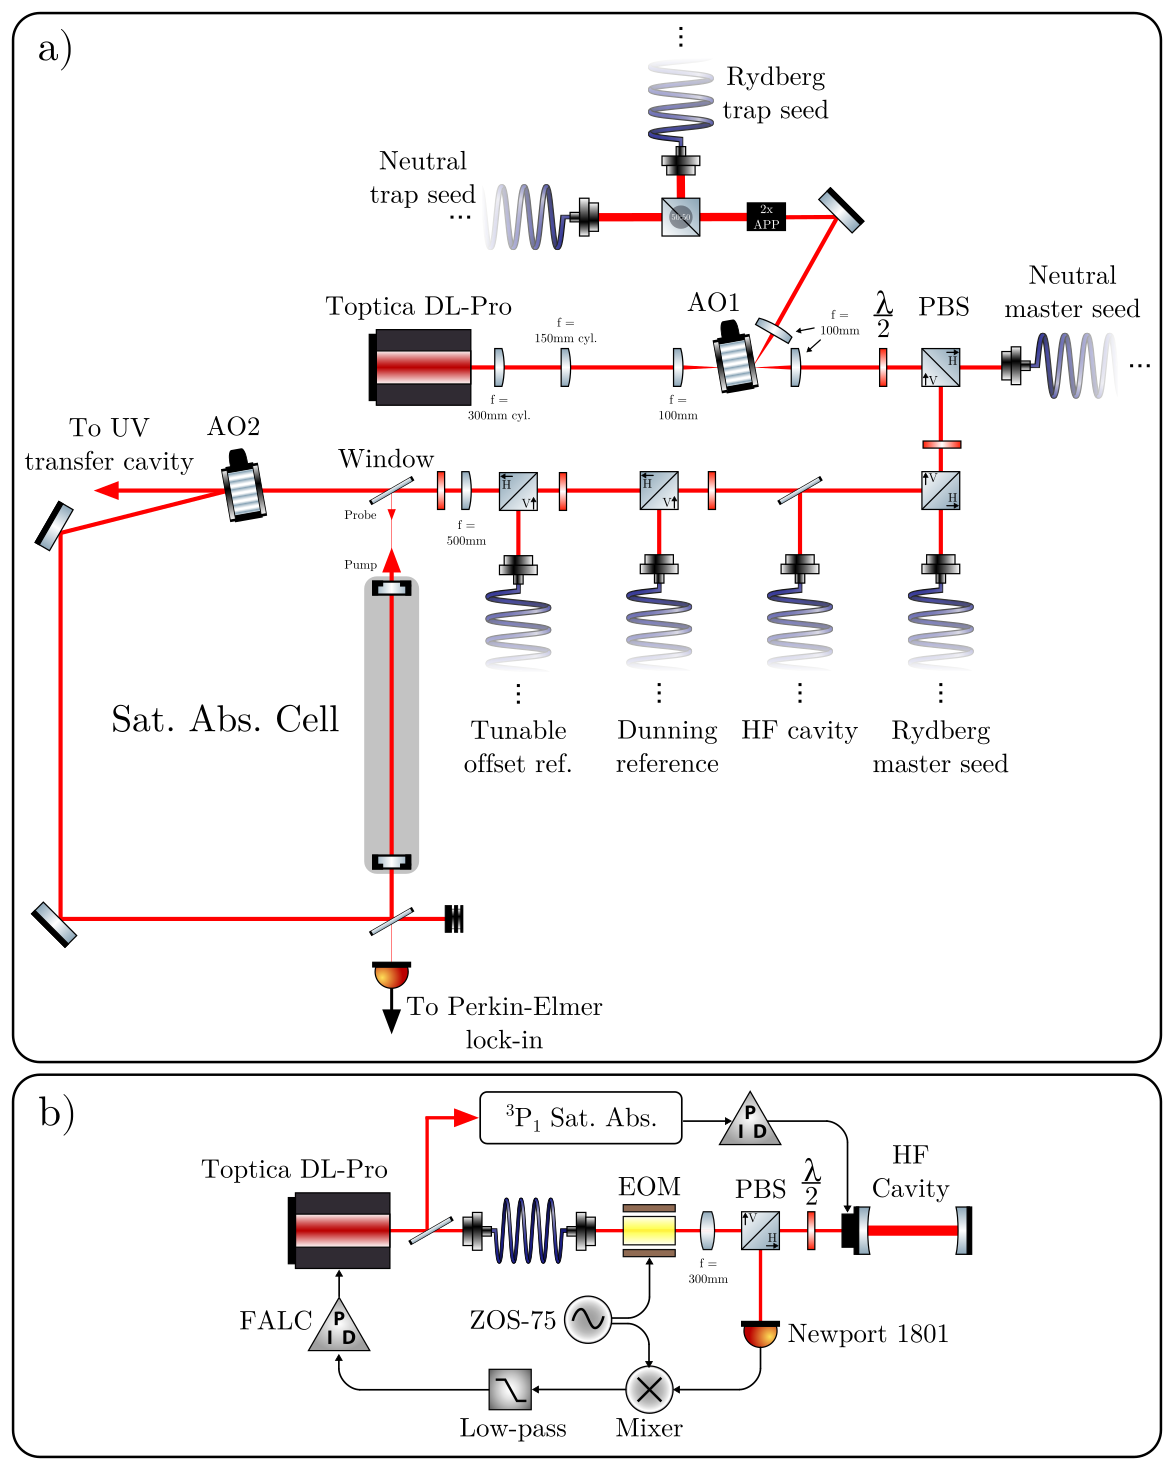
\includegraphics[width=\textwidth]{689_master.png}}
		\caption{689\,nm master optical setup}{The 689 master laser sees }
		\label{fig:689master}
	\end{figure}

%Description
%	Original reference
%Diagram
%Components
%	Mounts
%		Riser
%	Optics
%		Fiber mounts and launchers
%	Circuits
%		FALC connections
%		RF setup
%	Systems
%		High finesse cavity
%		Sat. Abs. 
%		Gigahertz AOM
%Typical running characteristics
%	DLC-Pro settings
%	FALC settings
%		Figures of linewidth
%		measurements of noise
%Profiles
%Tips for operation
%History
%
%
%Locking diagram

\paragraph{High finesse cavity}
The narrow linewidth of the intercombination transition makes it attractive for use in a slew of applications since it is trivial to detuning by thousands of linewidths using conventional acouto-optic modulators.
The conventional method to narrowing the linewidth of a laser is to use an extremely narrow linewidth optical cavity as a frequency discriminator.
Such high finesse (HF) cavities are common place in atomic physics experiments and practically required for any strontium experiments.

Locking diagram
The frequency is sabilized using by deriving an error signal from a saturated absorption cell.
	\begin{figure} 
		\centerline{
		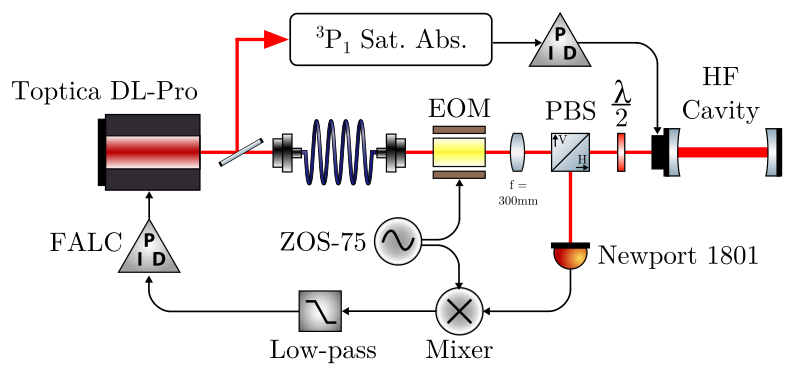
\includegraphics[width=0.6\textwidth]{689_StabilizationSchematic.png}}
		\caption{689\,nm master frequency stabilization}
		\label{fig:689freqLock}
	\end{figure}
	
	

\paragraph{689 sat. abs}
Optical shcematic
How much power?
We typically run at 400 \degree.
The frequency modulation is derived from the fast switching of the RF driving the sat. abs offset AOM.
The frequency

The remaining power from the master system outlined above is sent to a long heat pipe in order to interrogate the intercombination transition.
The error signal is generated using standard frequency modulated Doppler free saturated absorption as is done for the 461 system.
Fig something outlines the optical schematic for this system.
A maor difference compared to the 461 sat abs is the absence of a second pump(probe?) beam that is used to subtract off the Doppler broadened profile.
The red system is able to acheive this since the Doppler broadened profile is approx. 1 GHz compared to the natural line width of 7.5 kHz so any curvature due to the Doppler profile is not significant over the narrow linewidth.
In practice, it is difficult to acheive the transitions natural linewidth through this setup as a number of broadening mechanisms can dominate such as time-of-flights broadening and power broadening.
We find that our Lamb dip has a linewidth of approx. 300 kHz
We have attempted several improvements to narrow width but observe our Lamb dip to have a linewidth 


\paragraph{Measuring the laser linewidth}
Several important factors have seemed to conspire to limit the acheivable linewidth of the Toptica DL-Pro.
While we have pursued improvemenets to the laser system and attempted to maximize the locking badnwidth through short cables and commercial fast analog locking electronics, we find that the laser linewidth is limited to approx. 30 kHz.
Whereas similar implementations in various laboratories have reported laser linewidths of 1 kHz as readily achevieable \hl{refs??}.

Currently we attribute this large width to two main sources. 
First, the high finesse cavity is a homemade system and as reported in App. A.6 of Natali's thesis, has a linewidth of 200 kHz. 
Second, the cavity length is stabilized via interrogating the transition in a sat abs and where the locking signal linewidth is approx. 300 kHz.
Currently, a new ultra-low-expansion cavity is being tested and characterized to replace the homemade HF cavity which we hope will lead to a significant improvement in the laser linewdith.

The expected linewidth of the laser is quoted from Toptica to be on the order of 10 kHz.
However, this measurement is done using \hl{name of technique}, which requires extremely long optical fibers (on the order of 1 km) so it is not currently feasible to verify their claimed linewidth.
As we do not have the correct tools to measure the laser linewidth directly, we must rely on indirect measurements of atomic spectroscopy.
We performed two measurements through measuring the timescale for loss of coherence during a Rabi oscillation and confirmed through direct atom loss spectroscopy.
Fig something shows an example Rabi oscillation and the convergence of the decoherence rate as the lasr intensity is reduced.
While there are many sources that can contribute to the loss of atomic coherence, the dependence on laser power is suggestive.
Additionally, Fig something shows an example of atom loss spectroscopy at extremely low laser intensity.
The measured linewidth of this loss feature agrees with the 30 kHz obtained from the Rabi oscillation measurements.

COnvergence of timescale to a fixed linewidth?

\subsection{Neutral red system}
	\begin{figure} 
		\centerline{
		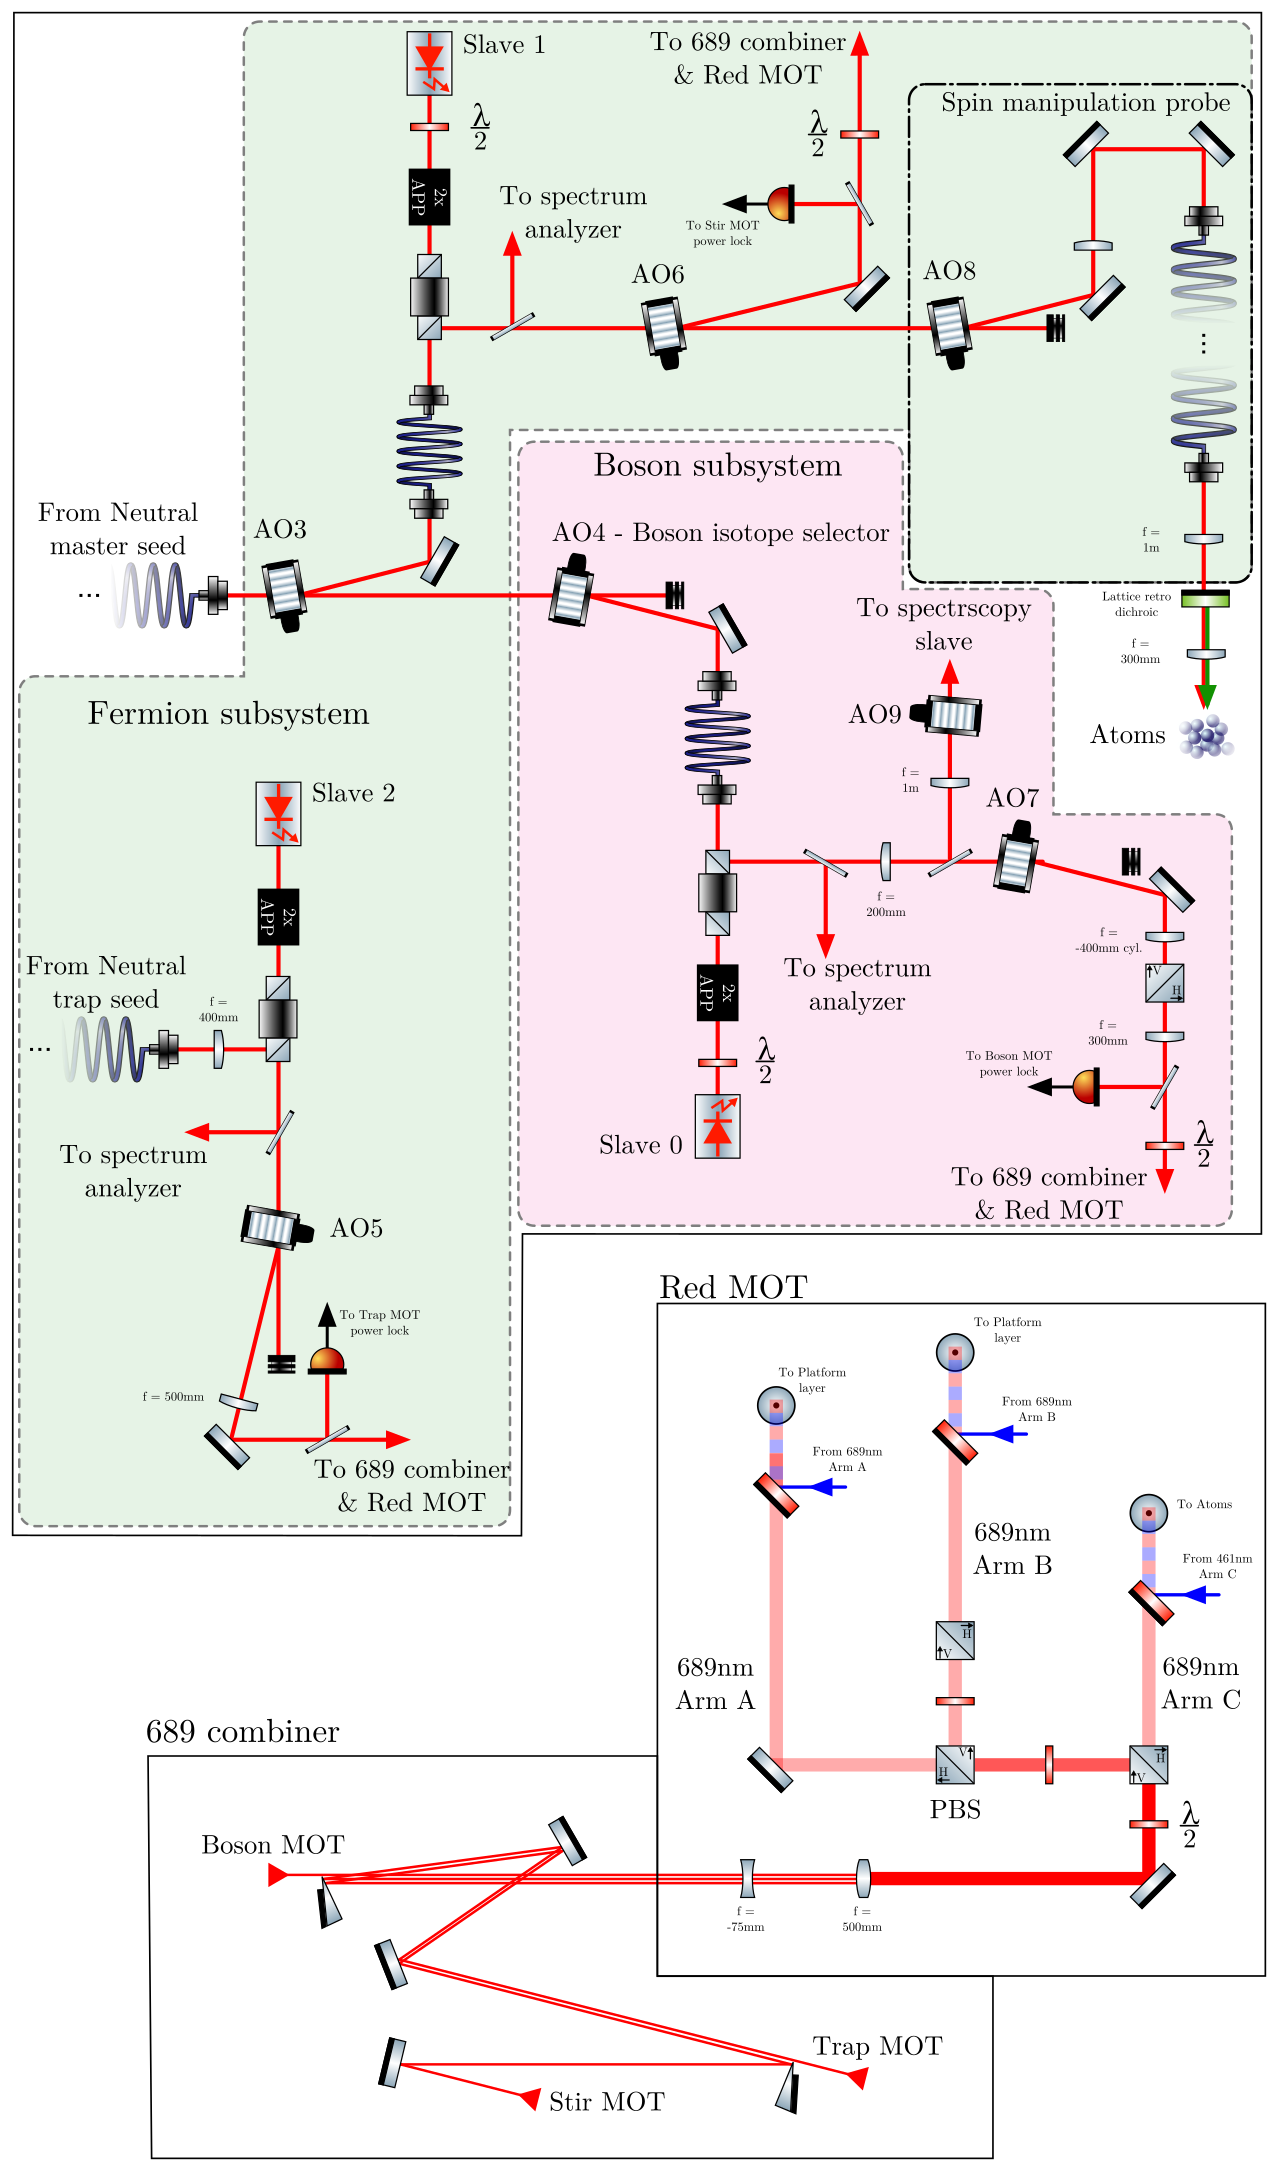
\includegraphics[height=\textheight]{689_neutralRedSystem.png}}
		\caption{Neutral 689\,nm trapping and cooling setup}{}
		\label{fig:neutralRed}
	\end{figure}
	
Light from the 689 master is directed to the Neutral experiment via a fiber connection.
From this approximately 3.3\,mW available at this output, we pass through two AOM's placed sequentially before separating out the requisite beams and directing them to the slave diodes for injection locking.

\subparagraph{Boson subsystem}
Fairly simple system with a slightly complicated method for switching between various bosonic isotopes.

Optical schematic and components
The boso

The 689 combiner + MOT path outlined in the figure is elaborated in figure.
This component is for overlapping the various laser beams which for the bosonic MOT, the fermionic trap and stir MOTs.

In order to change isotopes the aom of the boson selector must be changed according to something.
When swtiching between 88 and 84 this requires that the OMm be flipped around.
We have tested the reproducibility of this scheme and found it to be a simple of effective means for switching between various isotopes.
The MOT aom is run at a constant -82 MHz, therefore the three frequncies for choosing between the various isotopes are to land the input light to the blue of the the atomic trantion by 82 MHz.

Single mode oeration is monitored using spectrum analyzers 



%Description
%Diagram
%	Profiles?
%Components
%	optics
%		isolator
%		cubes
%		lensess
%	mounts
%		custom diode holder
%	aoms
%		RF circuits
%	circuits
%		temp controller
%		current controller
%	Spectrum analyzer
%		reference?
%		refer to the better version developed by Roger
%Runnign characteristics
%	Example spectrum?
%	MOT path powers

\subparagraph{Fermion subsystem}
Discuss the combination of all the paths using the D mirros and how you have to try and do the best you can with alignment. Typically found it best to align beams to center on the cubes and align to the chamber picking one of the paths. Then when adding additional path be careful to only touch the last two mirrors which independetly affect that path.


Description
Diagram
	Profiles?
Components
	optics
		isolator
		cubes
		lenses
	mounts
		custom diode holder
	aoms
		RF circuits
	circuits
		temp controller
		current controller
	Spectrum analyzer
Runnign characteristics
	Example spectrum?
	MOT path powers


Description
Diagram
	Profiles?
Components
	optics
		isolator
		cubes
		lenses
	mounts
		custom diode holder
	aoms
		RF circuits
	circuits
		temp controller
		current controller
	Spectrum analyzer
Runnign characteristics
	Example spectrum?
	MOT path powers
	
\subparagraph{689 combiner \& MOT}
Optical schematic of the combiner showing how the beams skirt by one another.
Long path lengths ensure fairly good co-propagation but it is not perfect.

The 689 combiner is a series of cloesly aligned mirrors for combining the boson, stir, and trap MOT beams before sending into the red MOT path and ultimately to the atoms.
Another popular way this is acheived is via fiber coupling but this is a lossy process.
Not perfectly aligned but it is good enough.

Give schematic
\pagebreak


\subsection{Optical dipole trap: 1064\,nm} \label{ssec:1064sys}
The 1064\,nm optical dipole trap is our primary science trap.
Since strontium has a J=0 ground state, magnetic traps that are common to alkali's cannot be used for trapping the strontium ground state.

There are two paths split, named the loading arm and the sheet/dimple arm as shown in Fig.\,\hl{some fig}.
Several diffferent types of traps have been formed, ref Ying thesis. 

How much power roughly is split between the arms?

AOMs are back to back which couples the power stability of the two arms. 
This setup allows us to more fully utilize the available power from the IPG and in practice while two completely decoupled independent arms may add a slight complication, when accounted for this has generally not been a major source of concern. 
Although, we have found it useful to continuously monitor the evaporation trajectory from shot to shot. 
As a problem, say with a misbehaving power lock, along one arm are is now coupled and may result in intensity fluctuations along both arms if the power lock cannot account for this perturbation.

Give stats on the loading path The loading path has the ability to be recycled on itself but we have not utilized this capability in many years due to complications of measuring the trap frequencies. 

The sheet/dimple arm can take two configurations as it's name implies. The sheet trap is an approx. 400 x 40um sheet with the short axis parallel along gravity. This geometry is useful for the low densities needed for Sr 86 to minimize the effecs of three body recombination. Alternatively, by switching out a mirror we can direct this power 

evaporation and description of density distribution
Formula for ramp
ref for where we get the formula and what it's purpose is

\subparagraph{Historical note:}
In the fall of 2018, the IPG YLRsomething, which had been in use for about a decade, died due to a thermal issue which led the internal fiber amplifier to overheat and burn.
As of April 2019, this laser is being replaced by \hl{something} and Josh Hill is reconstructing some elements of the paths reported here and in Ying's thesis.
Therefore, as his forthcoming thesis will outline this work in detail, we will focus our discussions on the general usage and procedures of the 1064\,nm trap.


\paragraph{Alignment Procedure} \label{sssec:1064_align}
Will focus on independent arm alignment of loading trap and sheet trap
Also useful to imagine three orthogonal axes with their origin set at the center of the chamber.
Fig.\,\hl{something} shows the propagation of the IR beams with respect to the science chamber


%% Loading
From the figure, we see that the loading trap propagates primarily along the X-direction. 
We start by aligning loading trap since it is generally less sensitive and the ports that it goes through are equidistance from the origin

Can generally get away with centering vertically on the chamber windows. 
goal is to rotate about the center point, can verify this by equalizing the distance from the edge of the window on both sides of the chamber
Letting the atoms extend along a single dimension of the trap. 
Moving the red MOT up and down with the z-trim. Dynamic control of z-trim is useful here as you can define a loading b field value then a science b field value.

As a secondary option, there are shortpass dichroic in place with fiber launchers positioned behind htem.
Use the shortpass dichoric mirrors to counter propagate a red loss beam. Alignment of the red beam follows the usual procedure making sure to reduce the exposure time and power as low as possible while maintaining a loss signal which should maximize alignment.


%% Sheet

%%%% Scratch
Best method is to copropagate with 689

The sheet trap propagates primarily along the y-axis. This direction has one port extended away from the main chamber body due to the ion gauge. This can complicate the alignment. You

is a little more complicated because it is very sensitive

For peaking up the the sheet trap alignment, hit the red MOT with the loading trap, then extinguish the red MOT away and hold in the single arm loading trap for approx 10-20ms. 
This allows the red MOT to fall away and the atoms caught in the ODT will expand along the arm, mapping out the spatial profile.
Once the untrapped atoms have fallen away, image the the atoms in situ (i.e. without a time-of-flight). 
With the spatial profile outlined you should be able to scan the sheet trap vertically looking for horizontal confinement along the loading trap. As the sheet is so tight along the vertical direction, this alignment is done using the last cylindrical lens before the chamber. 

Dimple trap follows the same process as the sheet alignment but there is a Newport Pico motor for finely adjusting instead of a lens.


\subsubsection{Trap frequency calibration} \label{sssec:1064_trap_freq}
Measurement of trap frequencies had previously relied upon parametric heating via intensity modulation of the optical dipole trap \hl{cite Ying thesis}. 
This process would observe atom loss via resonant heating when the modulation frequency matched a trap oscillation frequency. 
While this is a convenient and simple process it can lead to quite a complicated spectrum since the heating process does not discriminate directional information and may lead to coupling of higher harmonics of the trap frequencies. 

Recently, we have found excitation of center-of-mass (COM) oscillations to be a more reliable mechanism for measuring trap frequencies.
Fig.\,\hl{something} shows an example of trap frequency measurements taken via center-of-mass oscillations.

Vertical trap frequencies is a straightforward process whereby we can excite oscillations by quickly extinguishing the trap for $\approx$1-2\,ms before turning them back on.
By varying the evolution time once the trap is restored followed by a typical time-of-flight and absorption imaging, then we can observe the oscillations and fit the variation of the cloud center position over time to extract the frequency.
On a technical note, we find that this rapid on-off of the beams results in a brief overshoot of the power locks when turned back on.
However, the power lock equilibrium is restored after a few milliseconds and therefore we evolve for a time long compared to this perturbative behavior.

Exciting oscillations along the horizontal directions, X and Y, is a bit more challenging.
We have developed two mechanisms for exciting these modes which we call the kicking method and the pulling method.
The following sections will provide further detail.

\subparagraph{Kicking method:}
The kicking method has been primarily used for measuring the trap frequencies of the independent arm ODT.
In this configuration the two ODT beams are in plane and orthogonal.
This method is useful in this scenario since the excitation of the center-of-mass oscillation via an abrupt step of the AOM drive frequency.
This changes the deflection angle of the IR beam out of the AOM and "kicks" the cloud.
Briefly, the kicking procedure is 
\begin{outline}[enumerate]
	\1 During the ODT loading phase, load into a trap with one beam offset
		\2 The beam which is offset will excite oscillations along the opposite beam and measure the confinement due to the beam being shifted.
		\2 We have found that, in our current configuration, an offset of $\approx$1\,MHz results in a reasonable excitation amplitude.
	\1 Once the red MOT is extinguished and ODT loading is complete, we evaporate down to the trap of interest in the offset trap.
		\2 Here we find it useful to follow the evaporation trajectory for the experiment at hand. This is done so we can adequately model the potential and evaluate the trap depth.
	\1 After evaporation, we let the atoms equilibrate for $\approx$250\,ms then suddenly switch the frequency of the trap and hold for a variable evolution time before releasing and imaging.
\end{outline}

We achieve the frequency shift that excites the kick by stepping the input of a voltage controlled oscillator (VCO) which is typically fixed by a static voltage source.
During the experimental setup, we account for any voltage offsets between sources by measuring the output frequency of the VCO using an RF meter.
This is also ow we determine the needed voltage change for the $\approx$1\,MHz shift.

\subparagraph{Pulling method:}
With the recent addition of the high power 532\,nm for the optical lattice, we have explored an alternative method of inducing a center-of-mass oscillation. 
This method uses a single pass of vertically propagating green light (Arm C) to pull the atoms out of equilibrium and excite an oscillation.
Details of the setup are are given below in \ref{p:armCFirstPass}.

The pulling method has become our preferred method as it does not require us to change any AOM frequency sources as the kicking method has\footnote{Loading trap uses VCO so changing the voltage source is enough. However, the sheet/dimple is run from a IntraAction driver with a fixed digital synthesizer as the input. For this measurement we temporarily replace the synth with a VCO, but be careful as this will also change the gain of the power lock circuit (Synth outputs $\approx$0\,dbm but VCO outputs $\approx$10\,dbm)}.
Additionally, the pulling method can be applied to traps where the 1064\,nm light is recycled whereas previously our only recourse was te intensity modulation previsouly described.

\subsubsection{Modeling the potential} \label{sssec:1064_modeling}
Optical dipole traps result from the spatial dependence of the AC stark shift present whenever an atom interacts with a light field \cite{Grimm1999a}.
In the simple two-level dressed atom model, the AC stark shift originates from the diagonalization of the atom-photon system which results in an avoided crossing when the photon is nearly resonant with the difference between energy levels \hl{ref on dipole force as avoided crossing, CT book?}
Fig.\,shows a schematic avoided crossing near resonance where the separation between states is defined as $2\Omega$, or twice the Rabi frequency given by
\begin{equation}
	\Omega
	\label{eq:rabiFreq}
\end{equation}
From here we can understand the origin of the potential which provides the trapping force in ODTs.
To see this, consider an atom in the ground state, \ket{1}, and a light field with negative detuning, $\Delta < 0$.
Through the intensity dependence of Eq. \ref{eq:rabiFreq} we see that as intensity is increased the Rabi frequency also increases and correspondingly the energy of the ground state is lowered.
Conversely, when blue detuned, $\Delta>0$, the ground state energy is minimized in regions of low intensity.
The scaling of this change in potential energy is proportional to
\begin{equation} \label{eq:potProp}
	U(r) \varpropto \frac{\Gamma}{\Delta}I(r)
\end{equation}
where, $\Gamma$ is the natural linewidth of the transition determined by it's spontaneous decay lifetime, and $I(r)$ is the spatial dependence of the light intensity.

A subtle question may arise when considering the blue detuned case of Fig.\,\hl{some}.
If the atom seeks to minimize its potential energy, then doesn't the state \ket{2,n=0} represent a lower energy state?
To answer this, we must consider the scattering rate of photons which transition the atomic state from $\ket{1}\,\rightarrow\,\ket{2}$.
This rate is proportional to
\begin{equation} \label{eq:scatRateProp}
	\Gamma(r) \varpropto \left(\frac{\Gamma}{\Delta}\right)^2 I(r)
\end{equation}
Comparing Eqs.\,\ref{eq:potProp} \& \ref{eq:scatRateProp}, we find a favorable scaling for far off-resonant optical traps since the potential energy varies as $1/\Delta$ and the scattering rate varies as $1/\Delta^2$.
Therefore neutral atoms illuminated with high intensity off-resonant light will tend to remain in the ground state while feeling a trapping force, $F(\vec{r}) = -\nabla U(\vec{r})$.

As shown, the spatial dependence of the trapping potential derives from the TEM$_{00}$ gaussian intensity profile of the incident lasers given by.
\begin{equation} \label{eq:gaussInt}
	I(r,z) = \frac{2P}{\pi w(z)^2} \exp{\frac{-2 r^2}{w(x)^2}}
\end{equation}
where $z$ is along the beam propagation axis and $r$ is transverse to this axis.
Additionally, P is the incident laser power, $w_0$ is the waist radius at $z=0$, and the axial profile $w(z)$ is given by
\begin{equation}
	w(z) = w_0 \sqrt{1 + \left( \frac{z \lambda}{\pi w_0^2} \right)^2}
\end{equation}
where $\lambda$ is the laser wavelength.

Combining Eqs.\,\ref{eq:potProp} \& \ref{eq:gaussInt} we find the three dimensional potential generated by two orthogonal lasers to be given by
\begin{equation} \label{eq:indArmPot}
\begin{split}
	U(x,y,z) = m g z + \frac{2\alpha(\lambda)}{\pi} \left[ \frac{P_1}{w_1^y(z)\, w_1^z(z)} \exp{\frac{-2 (y^2+z^2)}{[w_1^y(z)]^2 \,[w_1^z(z)]^2}} \times \right. \\
	\left. \frac{P_2}{w_2^x(z)\, w_2^z(z)} \exp{\frac{-2 (x^2+z^2)}{[w_2^x(z)]^2\,[w_2^z(z)]^2}} \right]
\end{split}
\end{equation}
where $mgz$ accounts for the influence of gravity on the atoms of mass $m$, labels $1,2$ specify the lasers as illustrated in Fig.\,\hl{something}, and $\alpha(\lambda)$ is the AC polarizability of the ground state at a given wavelength.
This polarizability encapsulates the natural linewidth, detuning, and resonant behavior of the light field interaction with the bare atomic states \cite{Grimm1999a}.
Sec. 2.3.1 and App. A of Pascal's PhD thesis \cite{Mickelson2010b} outlines a calculation of the AC polarizability which at 1064\,nm is $\alpha( \lambda = \text{1064\,nm} ) = -10.9$\,Hz/(W/cm$^2$)\,$=-5.23\e{-8}$\,$\mu$K/(W/cm$^2$).
Units here are chosen as convenient lab units and can be converted to SI by $3.52\e{-40}$\,$\frac{\text{J}}{\text{Hz}}$\,(W/cm$^2$))$^{-1}$. 
Furthermore, $w_{(1,2)}^{(x,y,z)}(z)$ accounts for astigmatic laser profiles where the axial propagation along z of the orthogonal beam axes is not described by the same beam parameters.

The effects of gravity are a significant limiting factor for ultracold atoms as it is the dominant force that must be counteracted by the optical dipole trap.
Fig.\,\hl{something} shows the effects of gravity considering a simple one-dimensional gaussian potential, $U(z) = mgz + A\exp{\frac{-2z^2}{\sigma^2}}$.
Here we've chosen a general form of the gaussian for illustrative purposes.
From the figure, we see how to define the trap depth as the difference between the trap minimum and the lowest saddle point.
Furthermore, by making the harmonic approximation, shown by the dashed line, we can Taylor expand Eq.\,\ref{eq:indArmPot} and determine the expected trap frequencies.

From the lower figures we see realistic 3 dimensional profile of our independent arm ODT.
Analyzing the 3D profiles we find that the saddle points may not be along the line $z=0$, therefore we consider the full gradient when searching for the saddle point.
For deep traps (high power) the trap depth is well approximated by teh saddle point along $z=0$.
However, for this configuration at shallow traps (low power) the trap depth is determined to be along a non-trivial trajectory .
This realization has important implications for our analysis of the halo binding energy described in Ch. \ref{ch:chap3}.

\hl{want a 2 part figure. a) 1D plot of mgz+gauss with a harmonic overlaid. b) 3D deep trap. c) 3D shallow trap}

%then by illuminating an atomic sample with intensity light
%
%The separation between states is intensity dependent and using this we see the origin of optical dipole trap.
%
%Fig b shows the case of red tuning, as intensity is increased the separation between stats is increased and thus the ground state energy is overall lowered.
%This results in a varying potential energy surface which produces a force directing the atoms to the region of highest tintensites.
%Conversely, when blue detuned, the energy between states is decreased as the atom moves away from the laser intensity. 
%
% From Pascal
%The simplest dipole trap results from a single laser beam shone onto an atom. 
%A dipole moment is induced in the atom by the electric field of the laser, and the interaction between the laser field and the dipole moment of the atom means the atom experiences a force proportional to the gradient of the Stark shift (“light shift”) of its energy levels:
%Fdipole = -delta(delE) delr
%The gradient is along r which, for the usual Gaussian mode and radial symmetry of a laser beam, is zero at the intensity maximum of the laser and increases as the intensity drops off. 
%The energy levels move either towards or away from each other depending on the sign of the detuning of the light from the resonance frequencies of nearby atomic transitions, thus creating a potential that is proportional to the intensity of the laser:
%Udipole(r) prop Gamma Delta I(r).
%Here, Gamma is the spontaneous decay rate of a transition which is an amount Delta away from the laser frequency.
%Confinement also occurs in the direction of propagation of the optical trap laser if that laser is focused. 
%In that dimension, the maximum of the intensity will be at the waist of the optical trap beam. 
%For a single beam, however, the gradient tends to be much weaker longitudinally than radially, so the atom cloud elongates as the atoms take the shape of the trap. 
%The sign of the detuning plays a role as well (Fig.\,2.15): negatively detuned (red) detuned light moves the ground state energy down, so the trap becomes deeper. 
%But for positively (blue) detuned light, the opposite occurs, creating an anti-trap where atoms are driven away from the intensity maximum. 
%Equation 2.12 is the first of two expressions which encapsulate the key properties of an optical dipole trap. 
%Essentially, it specifies how deep the trapping potential of the optical dipole trap will be for a given laser intensity and frequency. 
%Losses due to scattering are the second important parameter characterizing an
%optical dipole trap. 
%Absorption, and subsequent emission, of light from the trap beam can heat atoms so that they are no longer trapped by the optical potential. 
%The losses due to scattering are also a function of the optical trap laser intensity and detuning,
%For an optical trap laser that is tuned on-resonance with an atomic transition (Delta = 0), both the scattering rate and the trap depth diverge, but the heating rate due to scattering is really limited by the rate that atoms can cycle from the excited state to the ground state. 
%The key difference from Eq. 2.12, however, is that Gammascat approx 1/Delta2, meaning that the rate of heating drops off more quickly with detuning than does the trap depth. 
%As a consequence, trapping neutral atoms in an optical dipole trap is feasible because we can usually find a laser intensity and detuning for which the trap depth is deep enough, but for which the scattering rate is not too high. 
%Finally, it is worth noting that squaring the detuning means that the loss rate is symmetric on each side of resonance, in stark contrast with the asymmetric behavior of Eq. 2.12.
%
%
%Basic theory
%	ac stark shift depends on intensity
%	gaussian beam intensity is spatially dependent
%		Formula for gaussian beam
%	this translates into a spatially dependent potential which can trap
%	must account for gravity
%		1D fig defining trap depth
%Applied
%	With this in mind we can use the above formulas to model the 3D potential from known parameters
%		get the polarizability from previous work by Pascal
%		reference appendix with explanation of program to do this
%	Make the harmonic approximation and solve for expected trap frequencies
%		compare expected and measured, typically get agreement within 10\%.
%	Once we have an accurate model we can find the trap depth
%		3D trap depth is a little more complex then the 1D analysis suggests
%		Fig of one deep 3D potential and one shallow 3D potential
%
%
%
%
%What is Li's different method?
%	he uses builtin jacobian function for finding the gradient matricies 


\pagebreak
\subsection{Optical lattice trap: 532\,nm} \label{ssec:532sys}
Until recently, experiments on the Neutral apparatus were confined to work with bulk gases in an optical dipole trap.
While optical dipole traps are useful for efficient evaporation and thermalization of an ultracold gas, optical lattices greatly extend our capabilites for studying ultracold molecules and novel many-body quantum states \hl{give some refs}.

Optical lattices are formed by a standing wave of light which creates a defect free periodic potential.
These traps are extremely versatile and have enabled the observation of the superfluid - Mott insulator transition \cite{Greiner2002}, artificial gauge fields for neutral atoms \cite{Lin2011}, quantum microscopy with single-site resolution \cite{Bakr2009}, and investigations of quantum magnetism \cite{Hart2015,Greif2015}. 
They are among the most well-established techniques for controlling a quantum state and have proven to be great tools for exploring the connection between few- and many-body systems \cite{Bloch2008}.

\paragraph{Background} \label{sec:latBackground}
An optical lattice is created by counterpropagating two laser beams to form a standing wave pattern, which for two plane waves in one dimension results in a periodic potential given by 
	\begin{equation}
		 V(x) = V_{lat} \; \sin^2(k_L x)
	\end{equation}
where $V_{lat}$ is the lattice depth determined by the polarizability of the atom for a given trapping wavelength $\lambda$ and laser intensity $I$, and $k_L$ is the lattice wavevector.
This potential can be readily extended to three dimensions using two additional pairs of counterpropagating laser beams along the $y$ and $z$ directions which results in a 3D cubic lattice.
Depth of the trapping potential, $V_{lat}$, is controlled by varying the intensity of the lattice beams.

Periodic potentials are powerful because they break the translational invariance of space which results in the formation of band structure and the opening of bandgaps or disallowed particle energies \cite{Ashcroft1976}.
Because of this broken invariance, $p$ is no longer a good quantum number and must be replaced by two new quantum numbers: the band index, $n$, and the quasimomentum, $q$.
In one dimension, quasimomentum is specified by $q = p - nG$, where $G=2\pi/a$ is a reciprocal lattice vector, and $a$ is the real space lattice constant.
Fig.\;\ref{fig:bandStructure} shows how the band structure varies as the lattice depth is increased.
Optical lattices have a lattice spacing $a = \lambda /2$ which determines the reciprocal lattice vector $G = 4\pi / \lambda = 2 \hbar k_L$ and the natural energy scale $E_r = \frac{\hbar^2 k_L^2}{2m}$ where $m$ is the atomic mass and $k_L$ is the lattice wavevector, $k_L = 2\pi / \lambda$.
From the band structure, we see that the bandwidth of each band, given by $\Delta E = E_{q=\hbar k_L} - E_{q=0}$, decreases as the lattice depth is increased.
In the limit that $V_{lat}\!\rightarrow\!\infty$ the band structure reduces to a ladder of harmonic oscillator levels spaced by $\hbar \omega_{ho} = \sqrt{4 V_{lat} E_r}$.
Although, for moderately deep lattices, $V_{lat} \gtrsim 5\,$E$_r$, this approximation is valid near the center of the Brillioun zone, $q = 0$, and provides a simple form to estimate the energy gaps between bands \cite{Jaksch1998,Jaksch2005}.
	\begin{figure} \label{fig:bandStructure}
		\centerline{
		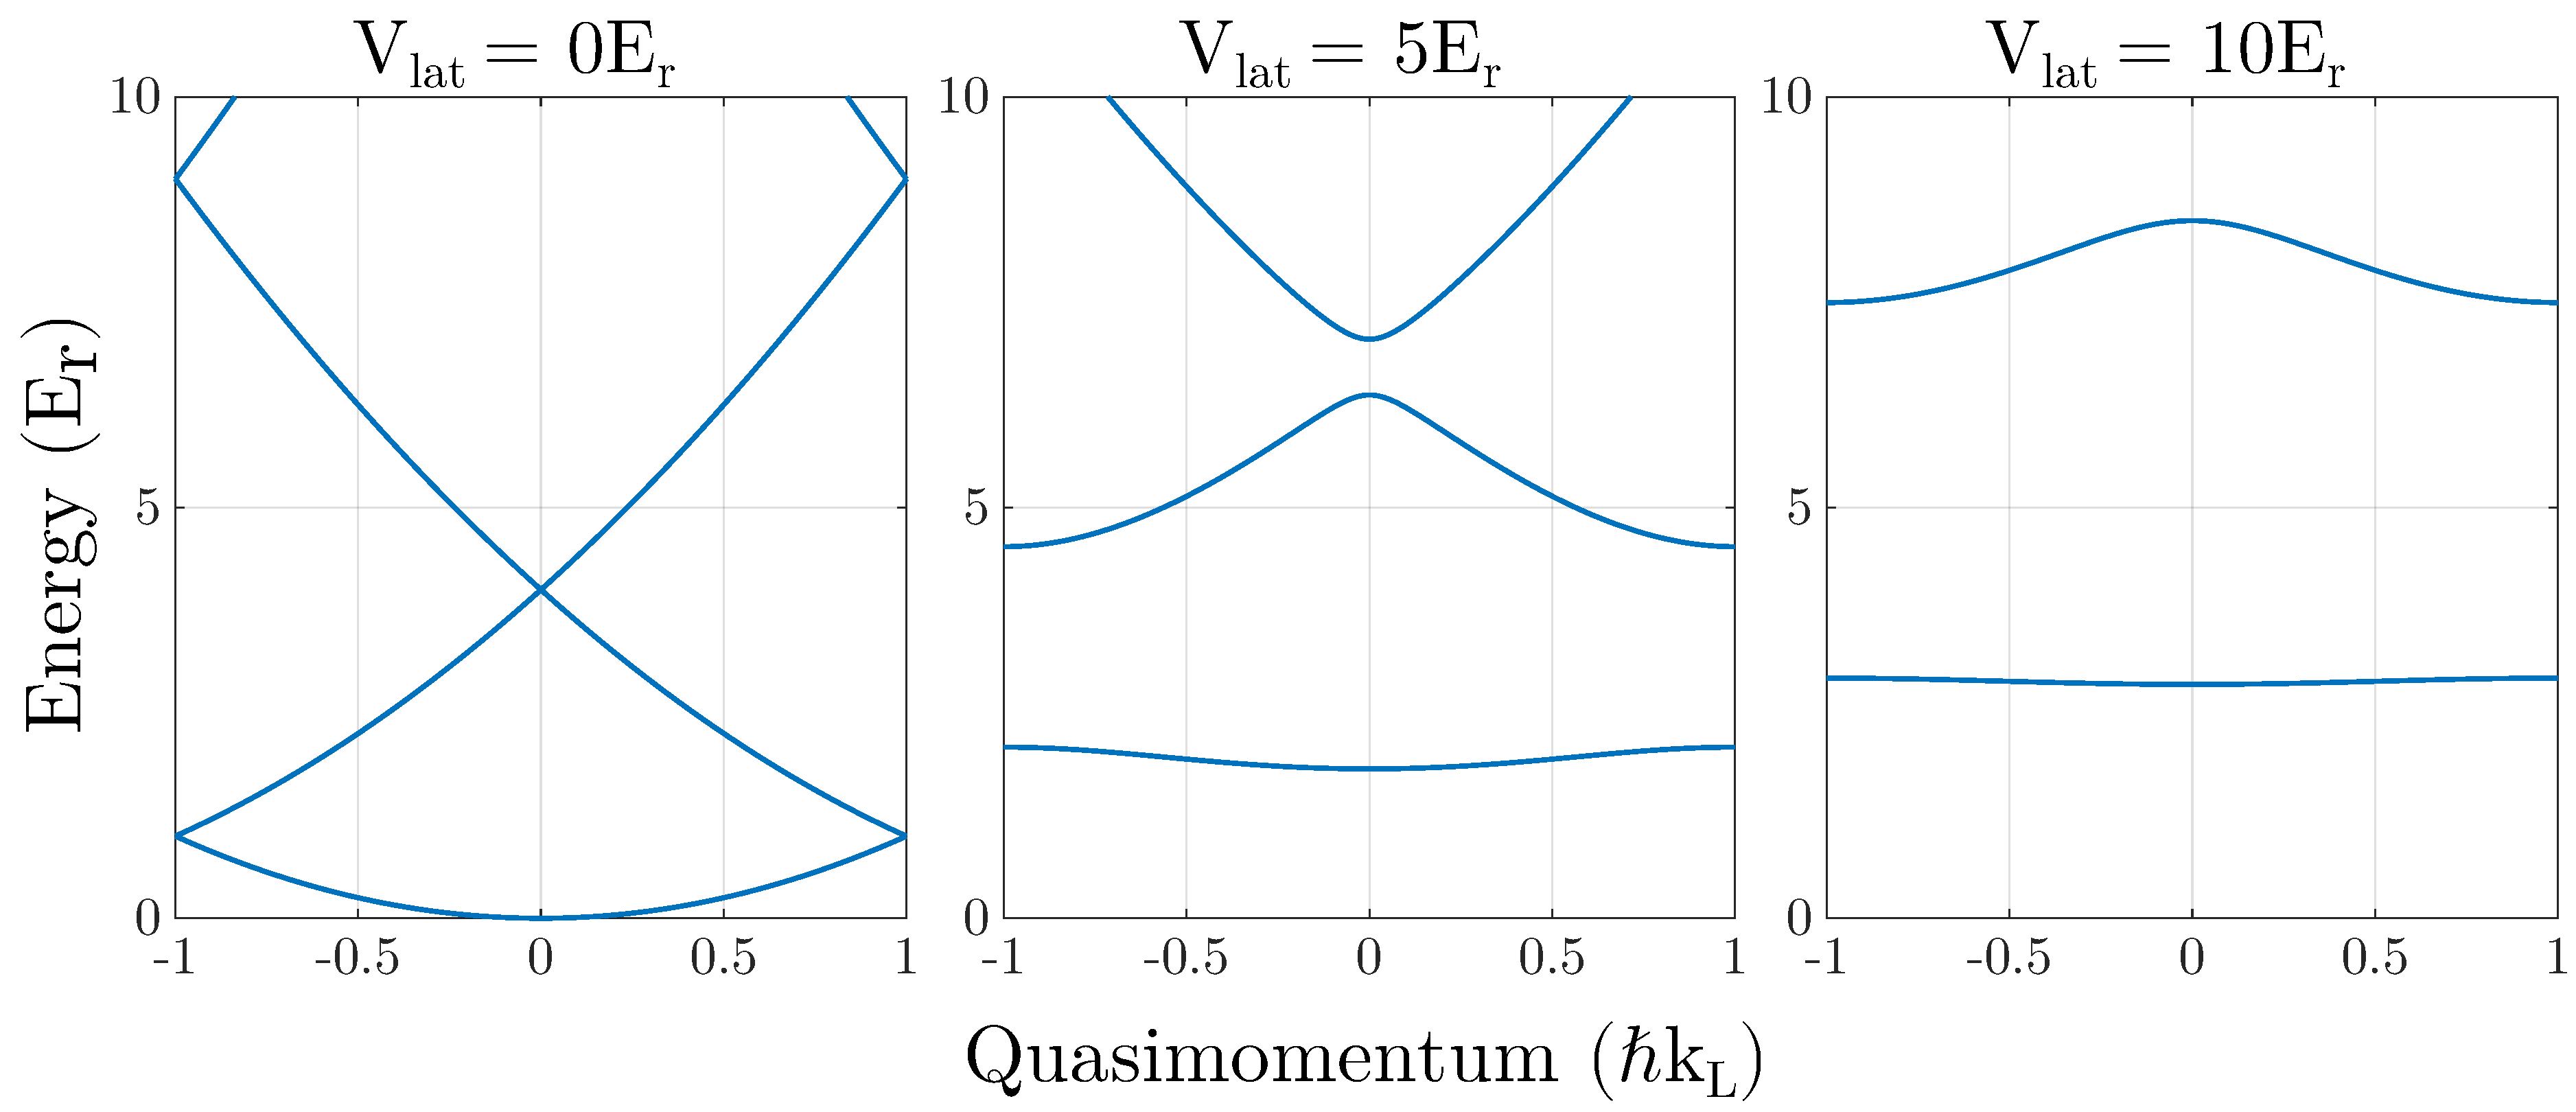
\includegraphics[width=\textwidth]{lattice_bandStructure.pdf}}
		\caption{1D band structure as a function of lattice depth}{One dimensional band structure for an optical lattice as the lattice depth is increased. The band energies are found by solving the Schr\"{o}dinger equation using the Bloch functions of Eq.\;\ref{eq:blochFunc}.}
	\end{figure}
Solutions to the Schr\"{o}dinger equation in a periodic potential are given by the Bloch functions \cite{Ashcroft1976}
	\begin{equation} \label{eq:blochFunc}
		 \phi_q^{(n)}(x) = e^{iqx/ \hbar} \; u_q^{(n)}(x)
	\end{equation}
These eigenstate wavefunctions are specified for a given quasimomentum $q$, and band index $n$. 
Their corresponding energy eigenvalues define the band structure of the lattice shown in Fig.\;\ref{fig:bandStructure}.
From Eq.\;\ref{eq:blochFunc} we see that the Bloch functions are the product of plane waves modulated by a function $u_q^{(n)}(x)$, which shares the periodicity of the underlying lattice potential \cite{Ashcroft1976}.
For an optical lattice this modulating function can be expanded in a basis of plane waves through a Fourier decomposition of the lattice potential in Eq.\;\ref{eq:1dlattice}, which gives \cite{Greiner2003},
	\begin{equation} \label{eq:blochMod}
		 u_q^{(n)}(x) = \sum_l c_l^{(n,q)} \; e^{i2lk_Lx}
	\end{equation}
Here $c_l^{(n,q)}$ are the coefficients for each plane wave in the basis expansion that are found by diagonalizing the lattice Hamiltonian \cite{Greiner2003}.

Often, we are interested in the dynamics of particles on a particular lattice site, but since Bloch functions are delocalized over the entire lattice, it is useful to instead use the Wannier functions. 
These functions provide an orthogonal and normalized set of wavefunctions that are maximally localized to a specific lattice site. 
The Wannier function for a localized particle in the n$^{th}$ band of a lattice site located at position x$_i$ is given by \cite{Jaksch2005}
	\begin{equation} \label{eq:wannier}
		 w_{n}(x - x_i) = \mathcal{N}^{-1/2} \sum_q e^{iqx_i/ \hbar} \; \phi_q^{(n)}(x)
	\end{equation}
where $\mathcal{N}$ is a normalization constant and $\phi_q^{(n)}(x)$ are the Bloch functions of Eq.\;\ref{eq:blochFunc}.
This localized description of particles allows us to calculate important physical quantities which govern dynamical properties of the lattice such as the tunneling rate, $J/ \hbar$, and on-site interaction energy, $U$. 
As $V_{lat}\!\rightarrow\!\infty$, the Wannier functions approach the eigenfunctions of the harmonic oscillator, which allows us to estimate the spatial extent of an atomic wavefunction by $a_{ho} = \sqrt{\frac{\hbar}{m \omega_{ho}}}$ \cite{Jaksch2005}.

\subsubsection{Setup and alignment} \label{sssec:532_align}

\paragraph{Setup}\label{ssec:lattice_setup}

Our optical lattice operates at $\lambda=532\,$nm and is derived from a Coherent Verdi V-18 single mode laser which is sent through separate AOMs for intensity control of each arm before propagating in free space to the atoms. 
We label these arm A, B, \& C as noted in Fig.\,\hl{chamber ref}.
The horizontal arms of the lattice ($x$ and $y$) have $1/e^2$ waists of approx $200\,\mu$m x $200\,\mu$m and their polarization is linear and aligned along the $z$ direction, parallel to gravity. 
The vertically propagating beam has a $1/e^2$ waist size of approx $300\,\mu$m x $300\,\mu$m and polarization aligned orthogonal to the polarization of the horizontal beams. 
With this configuration we estimate we can achieve lattice depths >$30$E$_r$ in an isotropic lattice. 

\begin{table}[]
\centerline{
\resizebox{0.95\textwidth}{!}{%
\begin{tabular}{@{}|c|llr|lr|@{}}
\toprule
 & \multicolumn{1}{c}{Label} & \multicolumn{1}{c}{Part} & \multicolumn{1}{c|}{Position {[}cm{]}} & \multicolumn{2}{c|}{Distances {[}cm{]}} \\ \midrule
\multirow{8}{*}{Arm A} & AOM & IntraAction AFM-804A1 & -126.5 & AOM$\,\rightarrow\,$A1 & 24.1 \\
 & PBS & Thorlabs PBS12-532-HP & -117.8 & A1$\,\rightarrow\,$A2 & 22.3 \\
 & Lens & CVI PLCX-25.4-772.6-UV-532 & -106.5 & A2$\,\rightarrow\,$A3 & 35 \\
 & Dichroic - 1 & Thorlabs HBSY12 & -30.6 & A3$\,\rightarrow\,$A4 & 4.5 \\
 & Dichroic - 2 & Thorlabs HBSY12 & 43.6 & A4$\,\rightarrow\,$AD1 & 10 \\
 & Retro mirror & CVI Y2-1025-0-0.30CC & 69.9 & AD1$\,\rightarrow\,$Atoms & 30.6 \\
 &  &  &  & Atoms$\,\rightarrow\,$AD2 & 43.6 \\
 &  &  &  & AD2$\,\rightarrow\,$ARM & 26.3 \\ \midrule
\multirow{10}{*}{Arm B} & AOM & IntraAction AFM-803A1 & -167.1 & AOM$\,\rightarrow\,$B1 & 19 \\
 & PBS & Newport PBS-5811 & -154.6 & B1$\,\rightarrow\,$B2 & 25 \\
 & Lens & CVI PLCX-25.4-772.6-UV-532 & 103.1 & B2$\,\rightarrow\,$B3 & 46 \\
 & Dichroic - 1 & Thorlabs HBSY12 & -36.1 & B3$\,\rightarrow\,$B4 & 23.5 \\
 & Dichroic - 2 & Thorlabs HBSY12 & 30.5 & B4$\,\rightarrow\,$B5 & 14 \\
 & Retro mirror & CVI Y2-1025-0-0.30CC & 73.5 & B5$\,\rightarrow\,$BD1 & 3.5 \\
 &  &  &  & BD1$\,\rightarrow\,$Atoms & 36.1 \\
 &  &  &  & Atoms$\,\rightarrow\,$BD2 & 30.5 \\
 &  &  &  & BD2$\,\rightarrow\,$B6 & 25 \\
 &  &  &  & B6$\,\rightarrow\,$BRM & 18 \\ \midrule
\multirow{6}{*}{Arm C} & AOM & IntraAction AFM-803A1 & -117.5 & AOM$\,\rightarrow\,$C1 & 45.5 \\
 & PBS & Thorlabs PBS12-532-HP & -109.5 & C1$\,\rightarrow\,$C2 & 25.5 \\
 & Lens-1 & CVI PLCX-25.4-772.6-UV-532 & -89.5 & C2$\,\rightarrow\,$C3 & 15 \\
 & Retro lens & CVI PLCX-25.4-149.9-UV-532 & 14.6 & C3$\,\rightarrow\,$C4 & 5.5 \\
 & Retro mirror & CVI Y2-1025-0 & 18.2 & C4$\,\rightarrow\,$Atoms & 26 \\
 &  &  &  & Atoms$\,\rightarrow\,$CRM & 18.2 \\ \bottomrule
\end{tabular}%
}}
\caption{Lattice optics details}{All measurements are specified in centimeters. The optics position is given with respect to zero defined at the atom position. Distances are referenced to the optics labels given in Fig.\,\ref{fig:532schematic}.}
\label{tab:532sys}
\end{table}

	\begin{figure} 
		\centerline{
		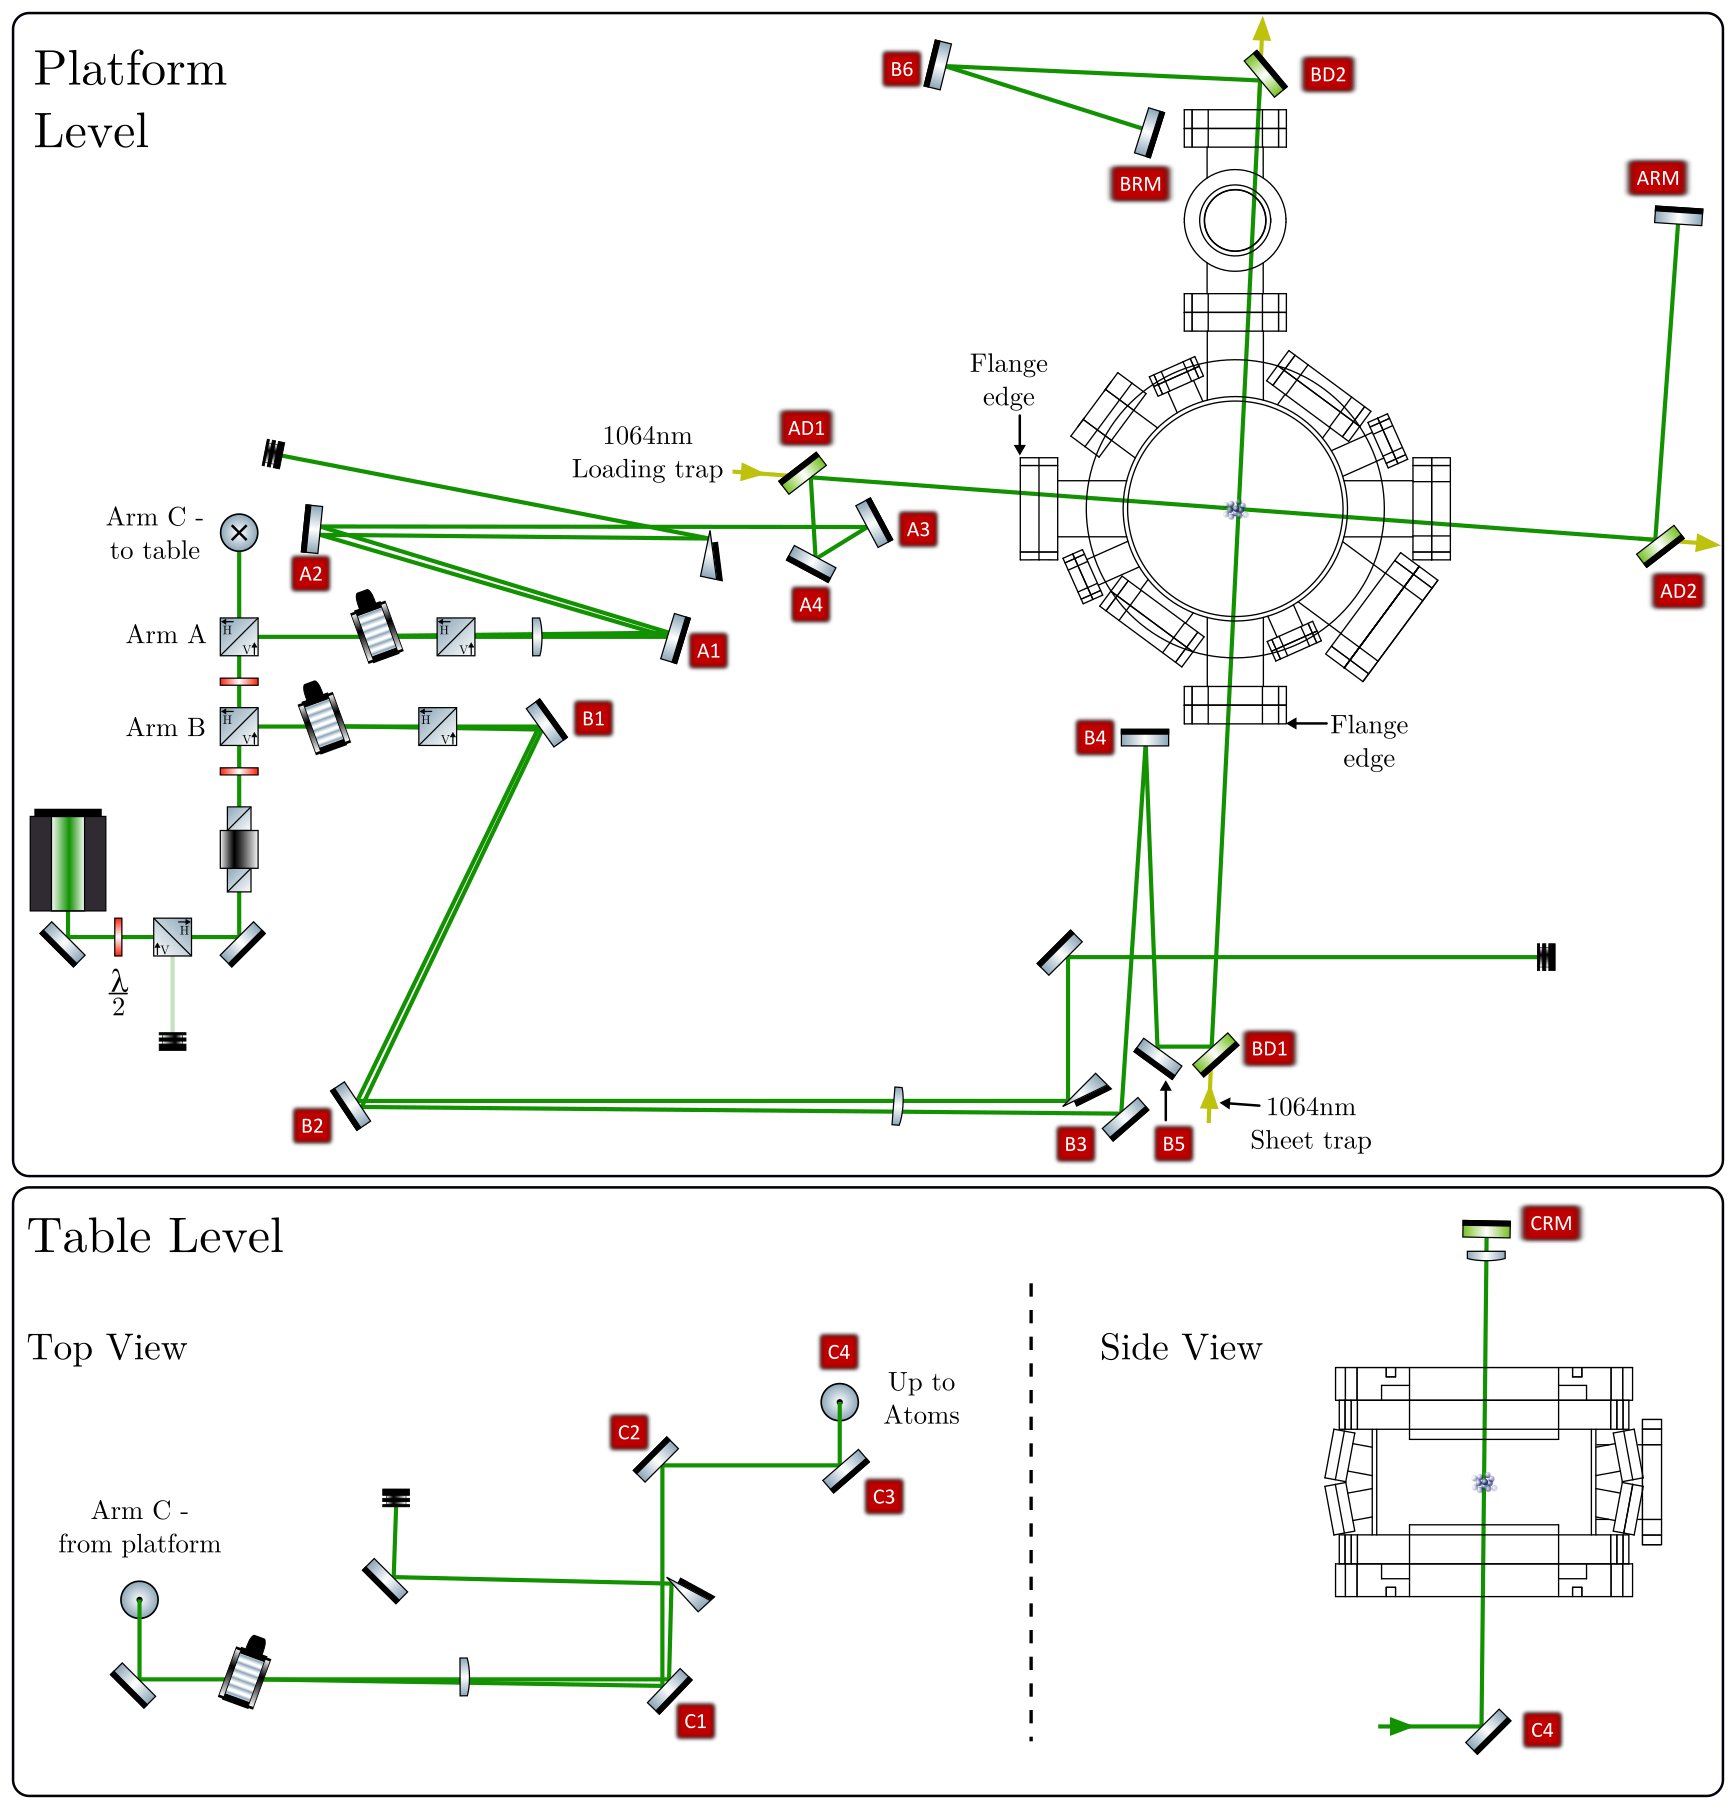
\includegraphics[width=1.2\textwidth]{lattice_schematic.png}}
		\caption{Lattice optical schematic}
		\label{fig:532schematic}
	\end{figure}
	
	\begin{figure} 
		\centerline{
		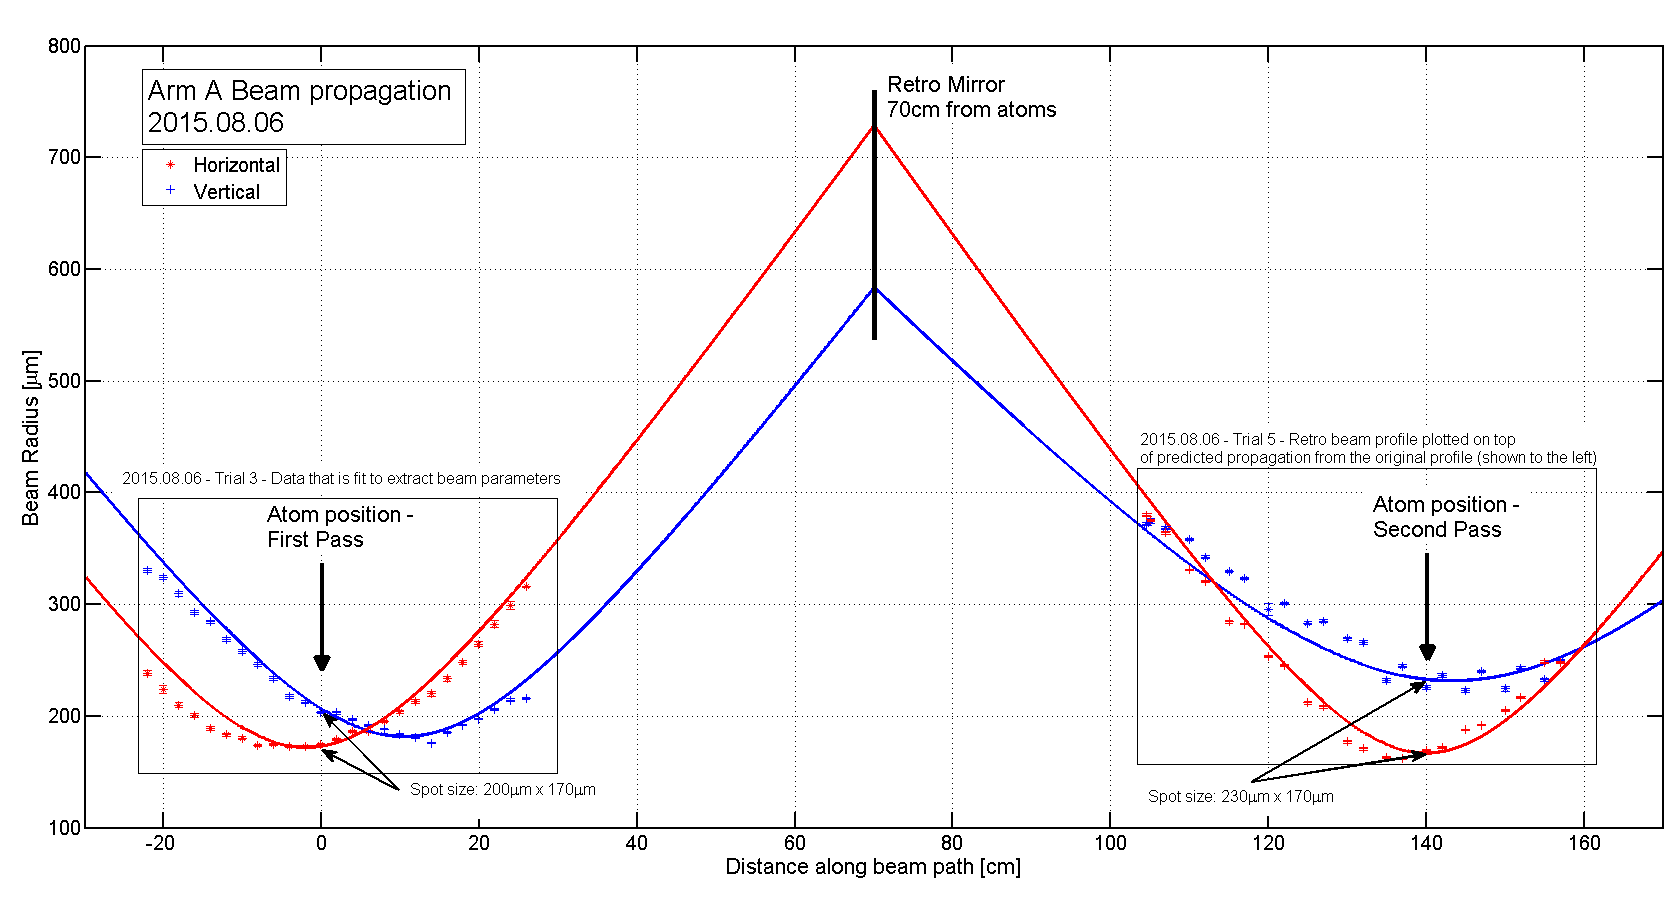
\includegraphics[width=\textwidth]{lattice_ArmAFull.png}}
		\caption{Lattice Arm A profile}
		\label{fig:532armAProfile}
	\end{figure}
	
	\begin{figure} 
		\centerline{
		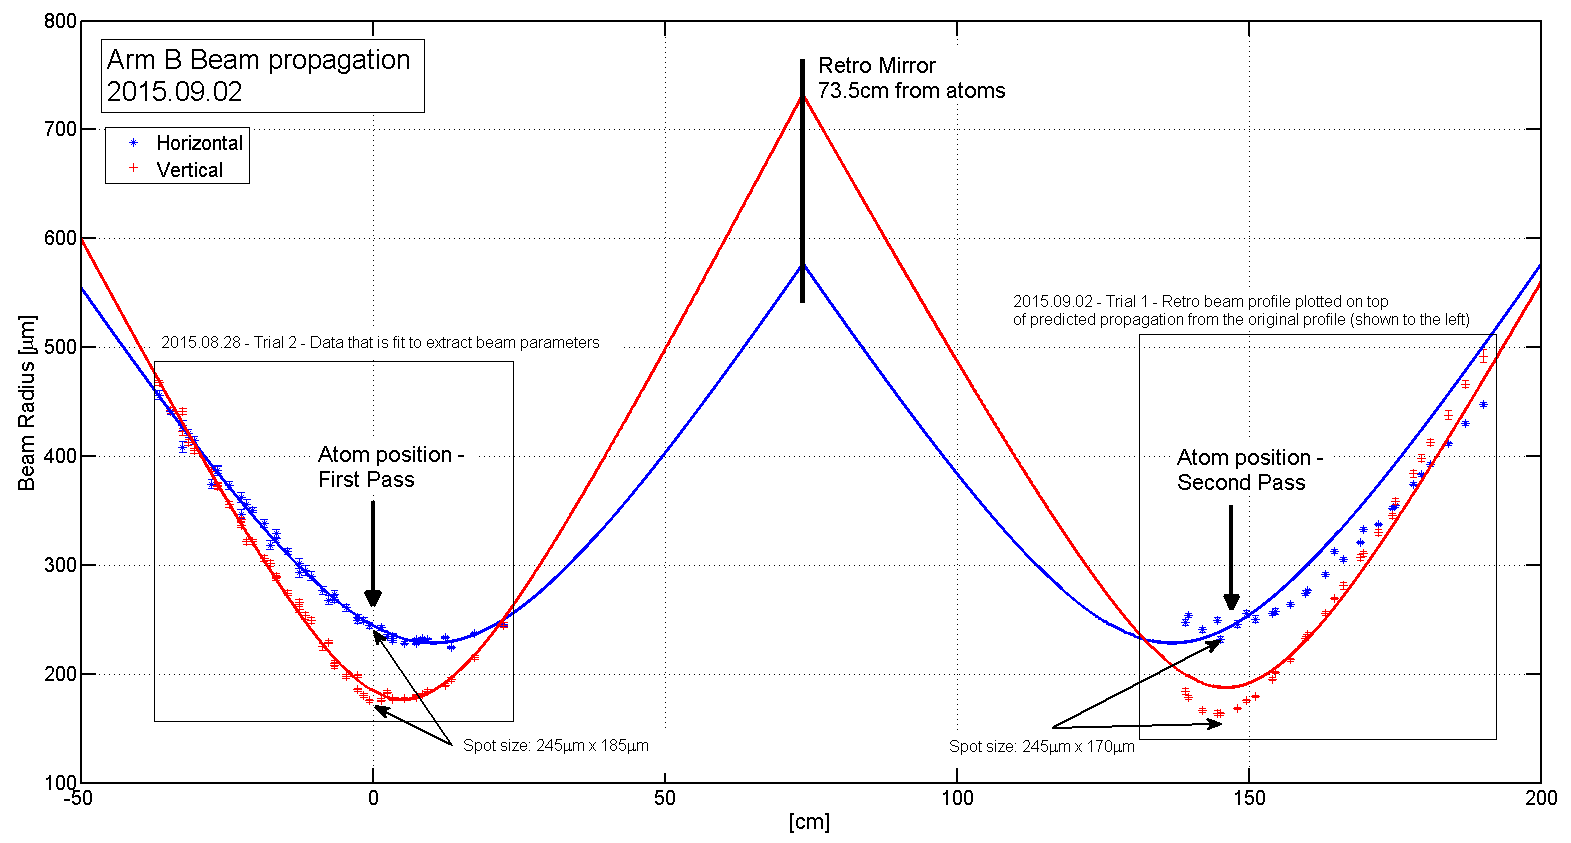
\includegraphics[width=\textwidth]{lattice_ArmBFull.png}}
		\caption{Lattice Arm B profile}
		\label{fig:532armBProfile}
	\end{figure}
	
	\begin{figure} 
		\centerline{
		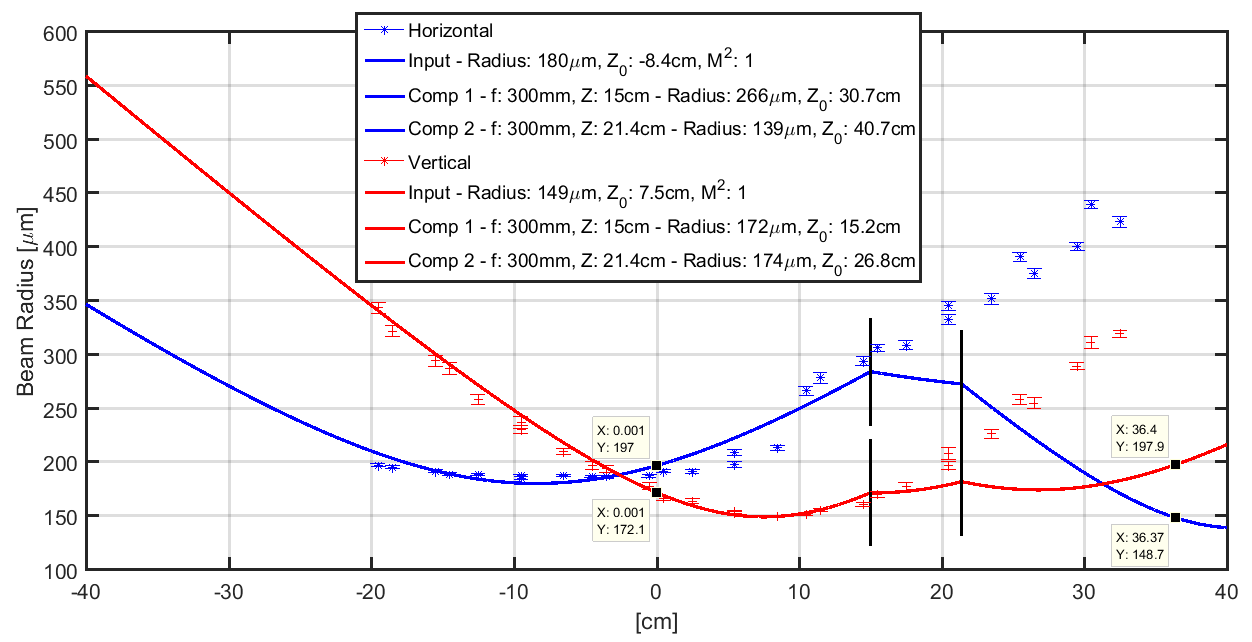
\includegraphics[width=\textwidth]{lattice_ArmCFull.png}}
		\caption{Lattice Arm C profile}
		\label{fig:532armCProfile}
	\end{figure}

\paragraph{Aligning the first pass:}
The following is a technique conveyed to our lab from Trey Porto.
We have successfully used this technique to align the first pass of the optical lattice and have found no better means of quantitatively determining the overlap of the 532 and 1064\,nm optical traps.
The basic idea is that when the beam centers are mis-aligned, the trap minima will be at a different spatial location.
Then by quickly turning off one of the beams (532\,nm in this case), we can cause quick shift in the minimum position, and thereby induce center of mass (COM) oscillates back and forth around the new minimum.
These oscillations are distinct from breathing mode oscillations where the COM stays fixed and the cloud's atoms move about it, expanding and contracting. 
These occur when the atoms are released from the lattice (though still confined to the ODT) and the new potential depth allows the atoms to pick up energy/velocity and oscillate.
We have observed these breathing mode oscillations to be present when the beams are well overlapped due to the change in trap depths (and correspondingly the potential energy of the atoms) when flashing off the 532\,nm light.

\begin{outline}[enumerate]
\1 This process requires the oscillations start from a consistent equilibrium.
We acheive this by te following experimental sequence:
	\2 Typical trapping sequence of blue MOT, repump, red MOT broadband, red MOT single frequency + ODT load
	\2 After loading the ODT, evaporate to a reasonable depth for the given loading time.
	Note that we have observed thermal effects from the ODT.
	Therefore, the point where the beam overlap should be optimized is at or near the desired trap depth for the proposed experiments.
	\2 Following the forced evaporation, hold in the 1064\,nm trap while ramp up the lattice arm being studied to full power.
	We generally find a ramp of approx. 200 - 300\,ms worked best for strontium 84. 
	\2 Once the green is at full power, we additionally held for approx. 250ms in the combined 532 + Crossed ODT trap to allow for the equilibration of the atoms in the modified trapping potential.
	\2 After the 250ms hold, the green is flashed off to excite an oscillation within the ODT.
	\2 Image the cloud as it oscillates
\1 To evaluate the procedure above, first focus on in-situ images of the cloud, where atoms are held in the combined 1064 + 532\,nm trap.
Start by moving the VI cursor positions to be on the cloud center and drawing a box around the cloud location.
This will help to identify small movements of the cloud as well as recording your start position.  
\1 When turning off the lattice and allowing the cloud to oscillate, identify the 1/4th period time of the oscillation. 
This is the point of maximum displacement and where we look to see if changes to the alignment are able to lower the oscillation amplitude.
As the alignment is improved the maximum displacement is minimized, this is the signature of improving the overlap.
If unsure about the oscillation period, scan the wait time after extinguishing the 532\,nm and observe the dynamics of the cloud to resolve a full oscillation.
\1 Each lattice arm (A,B,C) can then be varied in both dimensions (horizontal and vertical) while monitoring the oscillation amplitude. 
Lower amplitude indicates better alignment, but one must be extremely careful, as it is possible to obtain a flat signal by being so mis-aligned that the 532\,nm misses completely and no longer hits the atoms.
We have found that around the minimum in the oscillation amplitude, we are able to flip the phase of the 1/4 period oscillation as we move through the minimum.
This phase flip along with the emergence of breathing mode oscillation are robust measures of good overlap between the beams.
\end{outline}

Fig.\,\ref{fig:latFirtPass} shows an example of the above process.
Here we can clearly see that the amplitude of the oscillation is suppressed as we vary the beam pointing.
As taking this time series data is arduous, we would fix the wait time and observe the suppression as outlined above.
	\begin{figure} 
		\centerline{
		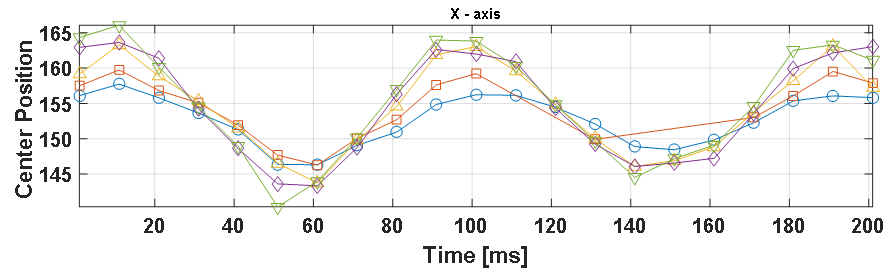
\includegraphics[width=\textwidth]{lattice_first_pass.png}}
		\caption{Center-of-mass amplitude suppression when overlapping traps}{Each subsequent scan is a single "step" in the pointing of the last mirror before the chamber. Note that the Y-axis is in arbitrary units.}
		\label{fig:latFirtPass}
	\end{figure}
	
\hl{Need to fix plot} Additional support for this method is seen in Fig.\,\ref{fig:latBreatheMode} which shows the emergence of a breathing mode when the traps are well overlapped.
In particular, we also see how reproducible this behavior is over a short time period (here about 20 minutes).
Day to day variation has not been found to be a limitation but further work must be done to ascertain the long term stability of the trap overlap.
	\begin{figure} 
		\centerline{
		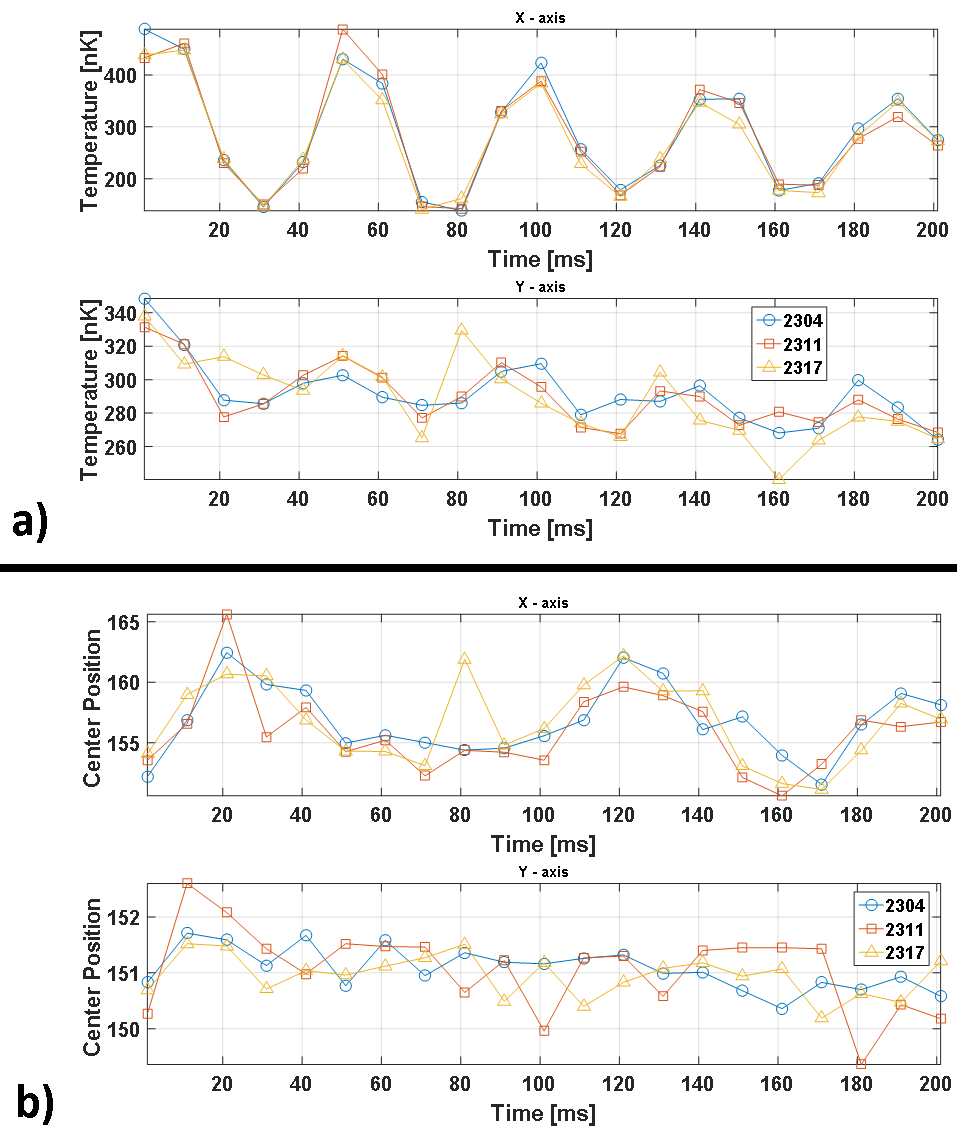
\includegraphics[height=0.8\textheight]{lattice_BreatheMode.png}}
		\caption{Emergence of breathing mode oscillation}{The measured radius and cloud centers in each axis of the absorption image. Observation of oscillatory behavior in X-axis without significant variation of the cloud center is a robust measure of the overlap of the 532 and 1064 traps. Once again, the Y-axis are given in arbitrary units.}
		\label{fig:latBreatheMode}
	\end{figure}
	
\subparagraph{Arm C:} \label{p:armCFirstPas}
The vertical path is special in all this.
We installed a special mirror as one of the last turning mirrors (give mode).
We have recently used this mirror to controllable pull the atom cloud in the 1064\,nm for performing trap oscillation measurements.
Describe using the separate program and it's limitations.
It is difficult to know we the beam is moving orthogonal to the IR beams but preliminary investigations show that small movements of the mirror axes couple predominantly along the independent IR arms.
This was deduced by performing a qualitative single point in time two-dimensional search where the in-situ cloud position was observed as the mirror position was varied.
A more quantitatively rigorous might be able to reveal the coupling between mirror axis by studying the time-series variation of the cloud center at each point of a two-dimensional mirror axis scan.


\paragraph{Aligning the retro-reflection:}
The retro-reflection is optimized via the 2-band Kapitza-Dirac method which is discussed below.
In short, for a quantum degenerate gas in shallow lattice depths, <10\,E$_r$, only the $\pm$1 plane waves will be populated.
Furthermore, for short pulses the amplitude of the population in these plane waves is linearly increasing with lattice depth.
This provides a simple single point measurement which can be used for optimizing the lattice depth.
However, an iterative approach may be needed to ensure that the alignment is only optimized during the first quarter period before the population of the orders is maximized.
Fig.\,\ref{fig:KDoscillations} shows an example oscillation.

As our lattice is free space, the first order alignment of the retro-reflection is to look over a long distance and overlap the incoming and return beam as best as possible.
This tends to overlap the two beams closely enough in the region of the atoms so as to observe some diffraction effects when performing a short high intensity pulse of the 532\,nm light.

Second, once we can observe diffraction, the gimbal mount retro mirrors are adjusted to maximize the population of the diffracted plane waves.
This alignment is extremely sensitive and may ultimately benefit from a more reproducible method of adjustment as mount backlash can strongly effect this process.
As the diffracted population is oscillatory and depends on laser intensity we have found that using an exposure time of approx 2 - 3 $\mu$s and varying the laser intensity has led to the most successful alignments of the retro.
We generally start at this short time pulse of a few microseconds with the highest intensity pulse possible and then systematically decrease the laser power into the lattice arm as the alignment is improved.
Finally we note that, as Kapitza-Dirac happens on very short timescales, the power stabilization circuits must be bypassed for this procedure.
Instead, we directly drive the RF sources with fast analog IC switches (switching time on the order of 10's ns) to apply the desired power to the lattice arm.

\subsubsection{Measurement and results}
\paragraph{Kaptiza-Dirac Scattering}
Kapitza-Dirac diffraction can be viewed as a diabatic projection from an initial eigenstate to a new set of eigenstates which results in an oscillation of the wavefunctions probability amplitudes over the new eigenstates of the system \cite{Denschlag2002}.
As was discusses in Sec.\;\ref{sec:latBackground}, the free space eigenstates are not the eigenstates of the lattice Hamiltonian. 
Thus a pure $p=0$ plane wave, $\ket{\phi_{p=0}}$, suddenly loaded into an optical lattice can be written as a superposition of the Bloch states given by Eq.\;\ref{eq:blochFunc}, here denoted by \ket{n,q}.
	\begin{equation} \label{eq:p0inBloch}
		\ket{\Psi(t=0)} = \sum_{n=0}^{\infty} \ket{n,q} \innerProd{n,q}{\phi_{p=0}}
	\end{equation}
The time evolution of this state is then given by
	\begin{equation} \label{eq:KDtime}
		\ket{\Psi(t)} = \sum_{n=0}^{\infty} \ket{n,q} \innerProd{n,q}{\phi_{p=0}} exp \left( \frac{-i E_n(q) t}{\hbar} \right)
	\end{equation}
where $E_n(q)$ is the energy of the Bloch state at a specified $q$ and $n$ shown in Fig.\;\ref{fig:bandStructure}.
The exponential factor of Eq.\;\ref{eq:KDtime} introduces oscillations among Bloch states and after a second diabatic projection back to the plane wave basis, we can relate evolution of plane wave population to the bandgap energy.
From this analysis we find that for relatively weak lattices, $V_{lat} \lesssim 10 E_r$, the plane wave population will vary as $\omega_{osc} = (E_2 - E_0) / \hbar$.
Where $E_i$ is the band energy of the i$^{th}$ band with $q=0$ as is the case when performing Kapitza-Dirac with a Bose-Einstein condensate.

Fig.\;\ref{fig:KDoscillations} shows a typical Kapitza-Dirac oscillation pattern which we use to maximize beam overlap near the atoms and calibrate our achievable lattice depths. 
Kapitza-Dirac is useful as an alignment tool since measurement of the population oscillation frequency can be highly accurate and directly relates to the bandgap energy in the lattice, shown in Fig.\;\ref{fig:bandStructure}. 
	\begin{figure}
		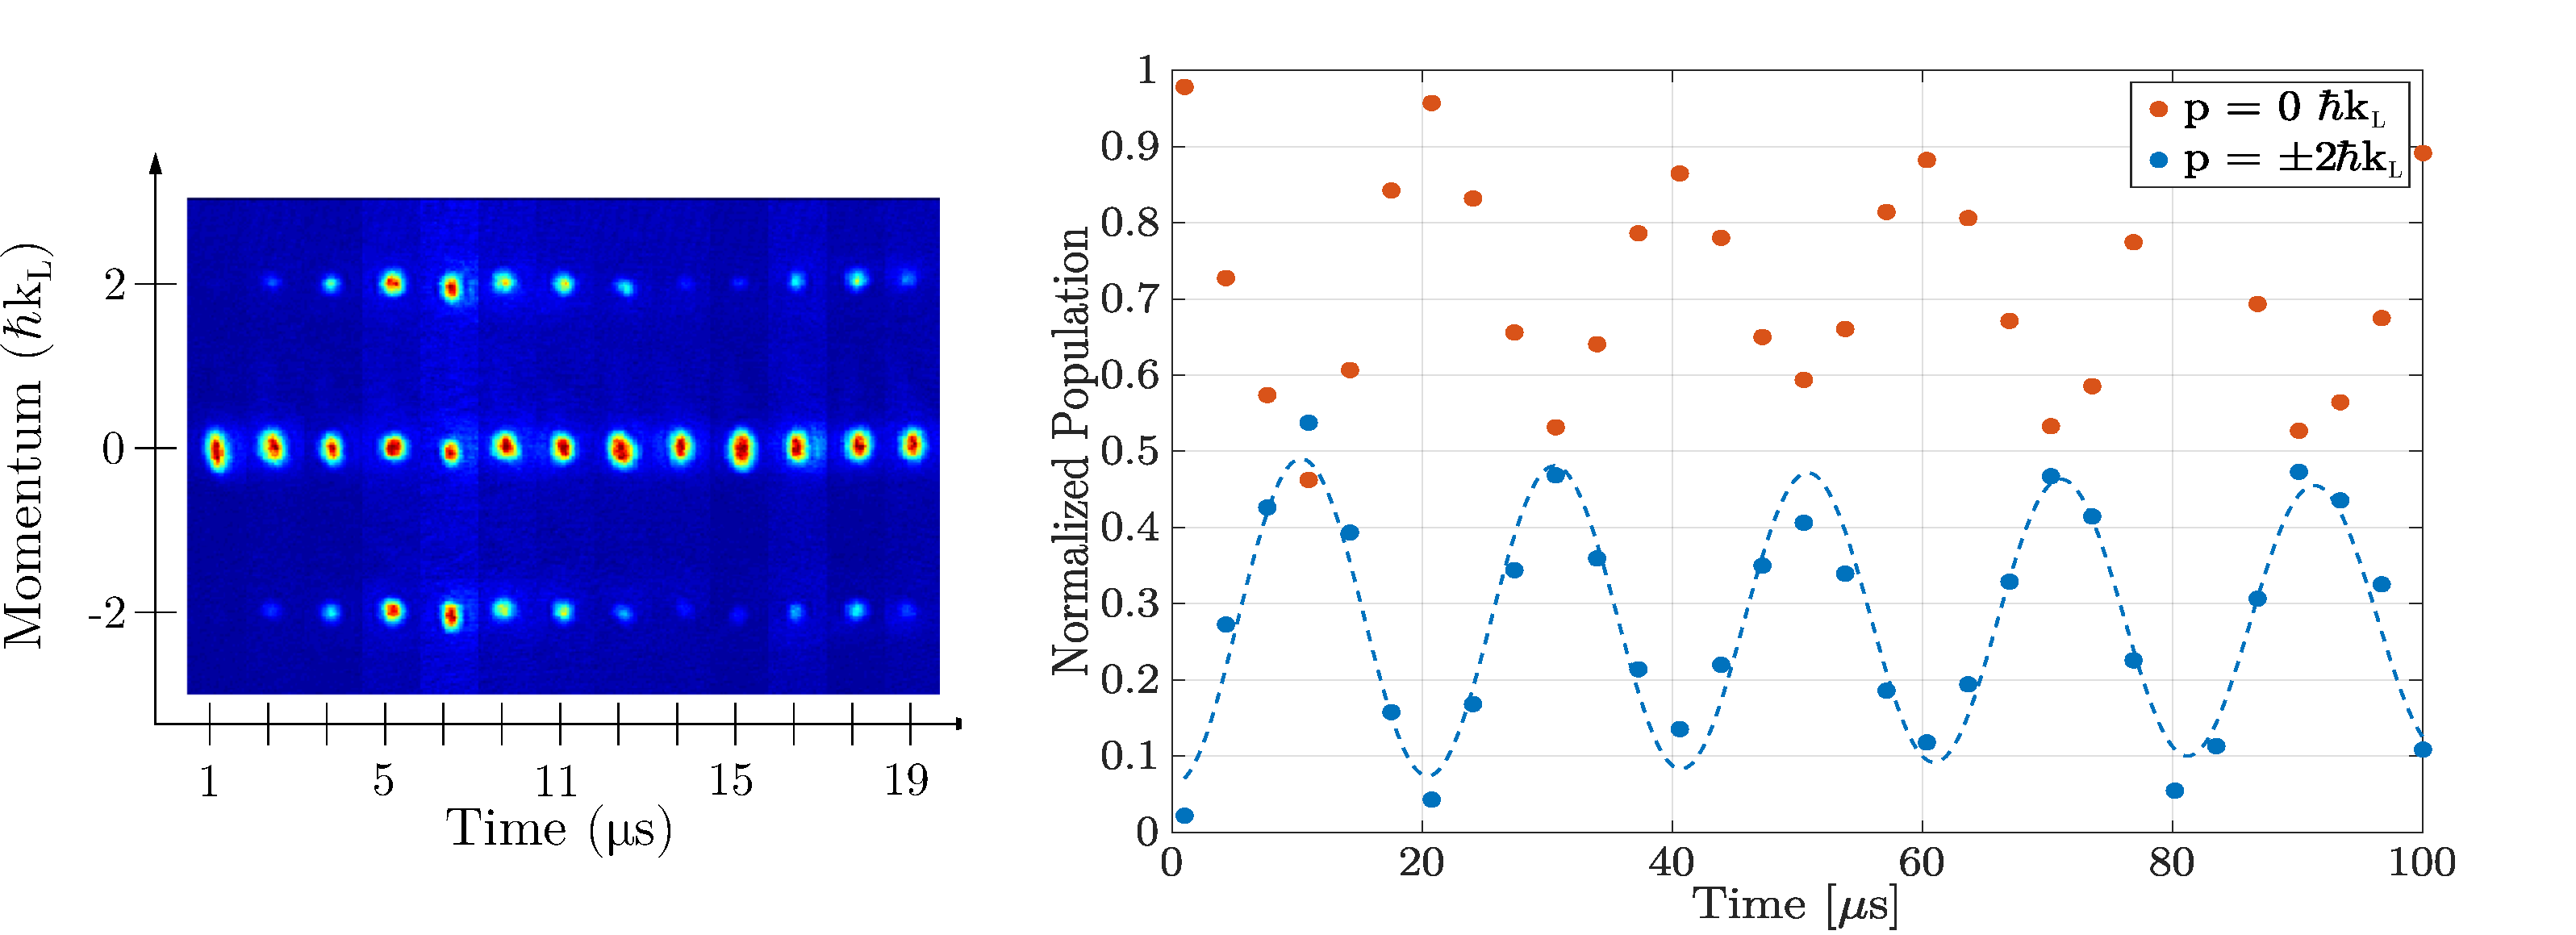
\includegraphics[width=\textwidth]{lattice_kdOsc.pdf}
		\caption{Evolution of plane wave population using Kapitza-Dirac}{Left: Time of flight slices for several realizations of Kapitza-Dirac with varying hold time in the lattice. Right: Normalized population from fits of time-of-flight images. Oscillations are fit with a decaying sinusoidal and the best-fit frequency is used to determine the lattice depth.}
		 \label{fig:KDoscillations}
	\end{figure}
	
	\begin{figure}
		\centerline{
		\includegraphics[height=0.4\textheight]{lattice_1DOscPeriod.png}}
		\caption{Oscillation period between $n=0\,\rightarrow\,n=2$ band at $q=0$}
		\label{fig:latOscPeriod}
	\end{figure} 
For reference, Fig.\,\ref{fig:latDepth} shows the resulting lattice depth calibration for our most recent alignment.
	\begin{figure} 
		\centerline{
		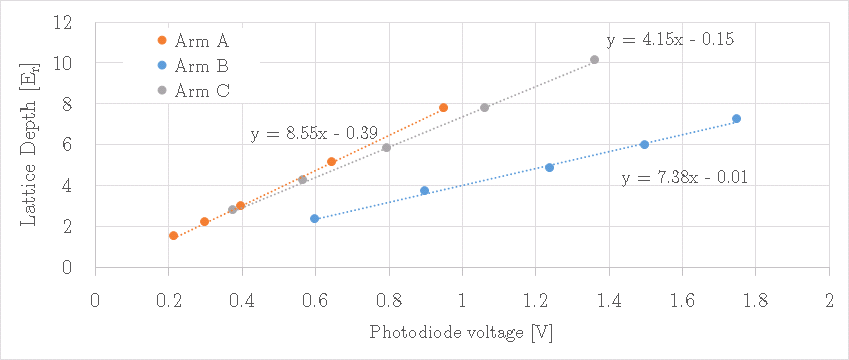
\includegraphics[width=\textwidth]{lattice_depth.png}}
		\caption{Lattice depth calibration}{Calibration was performed using the two-band Kapitza-Dirac technique. Maximum photodiode voltage for each arm is 10\,V}
		\label{fig:latDepth}
	\end{figure}
	
\subparagraph{Higher order Kapitza-Dirac:}
The simple two-band model given above is a straightforward method for determining the lattice depth but one that requires a time-series measurement over varying lattice depths.
Gadway et. al. \cite{Gadway2009} derived a complimentary depth calibration method which requires only a single time-series measurement at high lattice depth.
This process relies on the quantum interference of the oscillating populations which produces a complex beat note.
An undergraduate report from Alex Wikner \cite{Wikner2017}, follows the original Gadway construction to develop an algorithm using Matlab$^{TM}$ for applying this technique to the Neutral apparatus.
The cited report provides sample code as well as benchmark calculations for comparison.
However, application of this work to calibrate the lattice depth has been stymied by a consistent heating concern we have observed when applying the lattice beams for significant periods at high lattice depths.

\paragraph{Heating of a quantum degenerate gas}
While Kapitza-Dirac diffraction is useful as a characterization tool, we typically wish to maintain equilibrium when loading condensates into the lattice. 
Thus slowly ramping up the lattice laser intensity will adiabatically transform a plane wave ground state into the ground Bloch state of the lattice \cite{Sakurai2010}. 
Strictly speaking, in order to adiabatically connect the free space eigenstates and the lattice eigensates, the lattice must be turned on infinitely slowly due to the infinitesimal bandgaps which open near the band edges. 
Although near the band center, $q=0$, the adiabaticity requirement relaxes to $dV_{lat}/dt \ll 16E_r^2/ \hbar$, \cite{Denschlag2002} which for strontium in a 532\,nm lattice is $\approx 5\,\mu$s$/E_r$. However, in practice we find that our condensate fraction is reduced during fast ramps into the lattice. 

Instead, we slowly ramp on the lattice over 100\,ms which reduces heating caused by the ramp. 
We have experimented with various functional forms of this pulse shape and currently rely on an S-shaped curve given by Eq.\hl{somthing}.
\begin{equation}
	tanh
\end{equation}

As shown in Fig.\;\ref{fig:heatingRates}, we observe a large condensate fraction after similarly ramping the lattice back down. 
Additionally, by holding in a deep lattice after an adiabatic ramp, we can measure the effects of off-resonant scatter of lattice photons as a reduction of atom population over time.
For our red detuned optical lattice we expect the off-resonant scattering rate to be well approximated by a simple two level approach. In this model, the effective scattering rate is given by \cite{Jaksch2005}
	\begin{equation} \label{eq:offResScatter}
		\Gamma_{eff} \approx \frac{\Gamma V_{lat}}{\hbar \delta_{lat}}
	\end{equation}
where $\Gamma$ is linewidth of the dipole transition between the two states, $V_{lat}$ is the lattice depth, and $\delta_{lat}$ is the detuning of the optical lattice from the two level transition frequency.
In strontium, the $^1S_0\!\rightarrow\!^1P_1$ transition strongly dominates the polarizability of the ground state and therefore can be used to estimate the effective off-resonant scattering rate.
For this transition $\Gamma = 2 \pi \times 30.5\,$MHz and a 532\,nm lattice is detuned by $\delta_{lat} \approx 2 \pi \times 87\,$THz.
With a lattice depth of $V_{lat}=10\,$E$_r$ we expect a scattering rate of $\Gamma_{eff} \approx 2\e{-1}\,$s$^{-1}$, which is negligible for the timescales of our proposed experiments.
From Fig.\;\ref{fig:heatingRates}, we see that there is not an appreciable loss of atoms over a one second timescale, which at first would support our estimate that off-resonant scattering is unimportant on these timescales.
	\begin{figure}
	\centerline{
		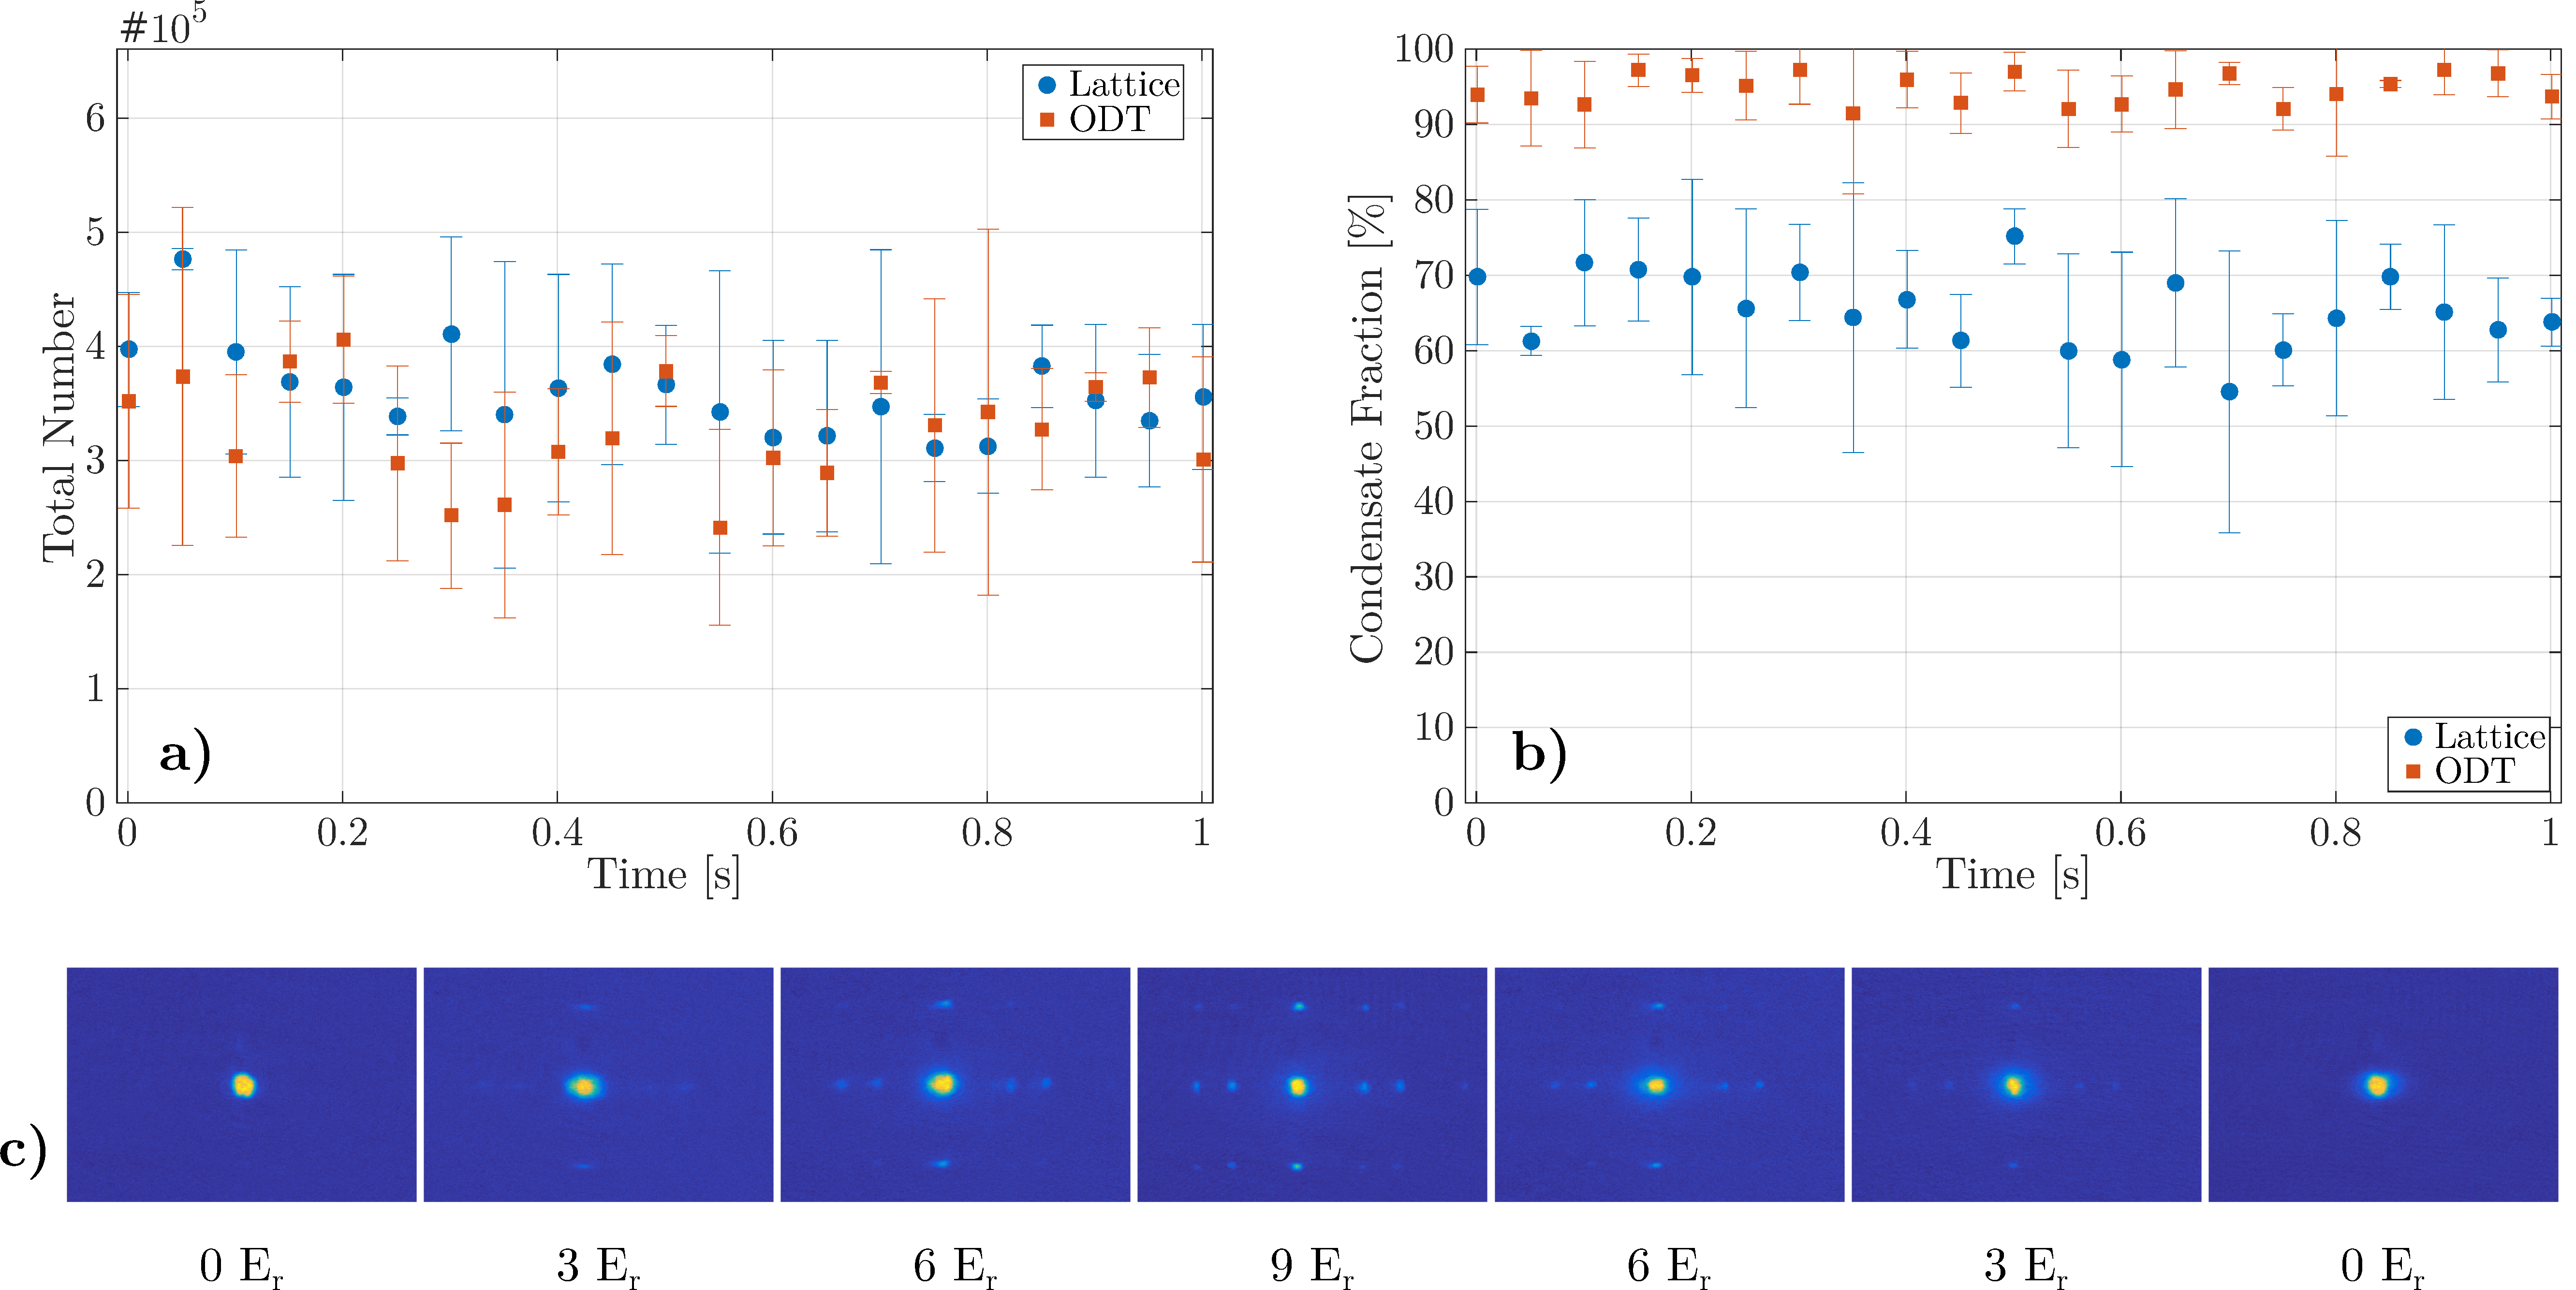
\includegraphics[width=\textwidth]{lattice_heatRates.pdf}}
		\caption{Characterization of heating in the optical lattice}{Evolution of condensate fraction over time after adiabatically ramping on the lattice to 9\,E$_r$. a,b) Comparison of total number and condensate fraction for a sample held in the optical dipole trap (red squares) or in a deep lattice (blue circles). c) Time of flight images after ramping on the lattice and diabatically projecting back to plane wave states.}
		 \label{fig:heatingRates}
	\end{figure}
Unfortunately, we have recently found that attempts to load a degenerate gas into a deep lattice, $\gtrsim 10$\,E$_r$, leading to unacceptable heating of the atomic sample.
Currently, we hypothesize that this may result from the freespace nature of the lattice or an intrinsic instability (frequency or power) of the Verdi.
The latter of these has been tested by monitoring the 532\,nm light in a spectrum analyzer where no obvious deficiencies have been observed.
To test the former hypothesis, we are currently investigating fiber coupling one of the arms of the lattice but as of spring 2019, this project is ongoing.

\subsection{Optical toolbox} \label{ssec:op_tools}
\subsubsection{Absorption imaging system}
Absorption imaging is a destructive measurement process which is predicated on measuring the spatially distributed attenuation of laser light after passing through an atomic cloud. 
In this section we will discuss the technical details of the Neutral absorption system and reserve the theoretical description of the process to Sec.\,\ref{ssec:tof}.
Additionally, we will reserve the discussion of image processing for App.\,\ref{app:imagefitManual} which details our software used to analyze the images and extract our physical measurements.

Fig.\,\ref{fig:absImagingSchematic} shows a simplified schematic of the absorption imaging system.
	\begin{figure} 
		\centerline{
		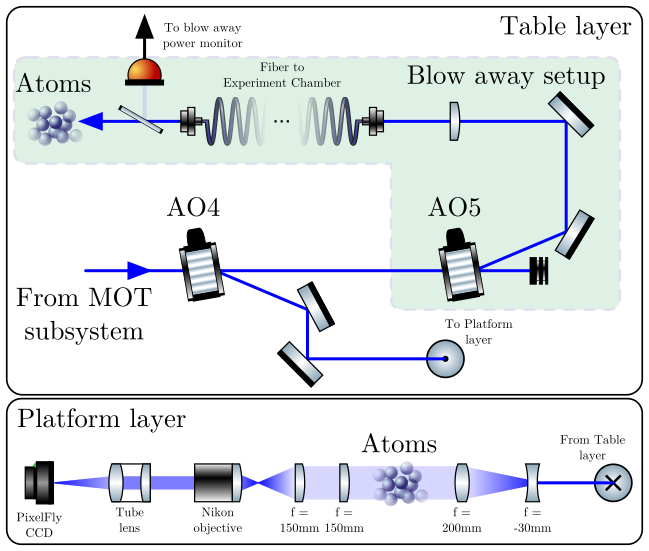
\includegraphics[width=0.8\textwidth]{461_imagingSchematic.png}}
		\caption{Absorption imaging and blow away pulser optical schematic}{Details on the contrsuction and characterization of the blow away setup are available in Josh Hill's masters thesis \hl{ref}.}
		\label{fig:absImagingSchematic}
	\end{figure}
Light is derived from the MOT path sub-system and guided to the atom chamber via freespace propagation. 
After passing through the atoms an imaging system shapes and focuses the image onto a Cooke PixelFly CCD camera.
The PixelFly is a 12\,bit 1280x1024 CCD with a pixel size of 6\,$\mu$m.
The imaging system after the atomic sample was developed by Mi Yan and is outlined in detail in App. A of his PhD thesis \cite{Yan2013d}. 
Much of the imaging sequence is a standard procedure that does not change day to day.
However, there are a couple of technical issues that may affect the operation of this system which we'll outline below.

First, it is important to not overexpose the image through saturating the camera's pixels by applying the imaging laser for too long.
We typically expose for 5\,$\mu$s with sample optical depths around one.
Due to drifts in the power output of the MOT cavity, we must occasionally increase the exposure time.
The figure of merit for determining the exposure time, is to expose just below saturation around the edges of the image\footnote{The auto-ranging color axis in the Labview VI is useful for quantitatively determining what the maximum pixel count is, then just keep it near but just below $2^{12}=4096$}.

The second consideration when taking images is related to how we extract the optical depth from images, the physics of which is discussed in Sec. \ref{something}.
For now, we will take as a given that each experimental sequence requires one image with the atoms in frame and another background image without the atoms.
In the ideal scenario these two images would be identical except in the region of the atom cloud and thus information about the cloud could be inferred using Beer's law \hl{ref}.
However, practically we must wait for the atoms to exit the frame and thus introduce a time delay between between the consecutive images that we seek to minimize.
For this reason we utilize a special feature of the PixelFly called "double-shutter" mode.
This particular imaging mode of the camera utilizes a second hidden set of pixels that are interleaved with the active pixels of the CCD.
Typically the acquisition time between consecutive images taken with a CCD is limited by the analog-to-digital conversion time needed to readout the image from the pixels into the camera's memory.
However, the PixelFly's set of hidden pixels lets the first image that is taken simply shift one row down from the active pixels into the hidden ones once the externally triggered exposure time has elapsed.
Once shifted down, the active pixels are free to be exposed again.
With this process the time between images is reduced to 5$\mu$s.
Fig.\,\ref{fig:pixelflyTiming} shows a full overview of this process.
	\begin{figure} 
		\centerline{
		\includegraphics[width=0.6\textwidth]{misc_pixelflyTiming.png}}
		\caption{Timing diagram of PixelFly doubleshutter mode}{t$_j$ refers to timing jitter inherent to the camera. In this scheme the first exposure can be controlled via the external trigger but the second image exposure is fixed to the readout time of the first image.}
		\label{fig:pixelflyTiming}
	\end{figure}
The drawback of this scheme is that for exposure times less than the readout time of an image, the second image is forced to have a minimum exposure of the readout time.
This presents a challenge as our exposure time is about four orders of magnitude faster than the readout time.
To overcome this, we rely on the fast response of the imaging system AOMs, a high extinction ratio of the 461\,nm photons, and a narrow line filter centered at 461\,nm attached directly to font face of the CCD.
Fig.\,\ref{fig:absImagingSchematic} shows two AOM's along the imaging path before the atoms.
We found two AOM's necessary to attenuate leakage light along the path to acceptable levels while maintaining fast response times which a physical shutter cannot replicate.

Great care is taken to reduce the time between images since the laser intensity and frequency might drift between the atom and background images. 
Variations in intensity have straightforward implications for errors since the measurement of the atomic number density assumes the only difference between the images is due to the presence of scattering particles, Sec.\hl{some sec}, and does not account for fluctuating photon number. 

The more insidious source of error in absorption imaging is variation of the optical frequency. 
Coherent, frequency stabilized radiation is used to illuminate the atom cloud so that we may control the optical absorption cross section and accurately measure the atomic number density. 
However, this laser light is passed through many optical components on it's path to the atoms and ultimately the imaging camera. 
Small reflections along this path result in a multitude of interferometers which causes small scale spatial intensity variation across the beam. 
Exacerbating this problem are short time frequency drifts that may occur between the atom and background images which result in slightly different fringe patterns in the atom and background images. 
Fringes patterns are a well known nuisance in experimental AMO images and it has become routine to use linear algebra techniques (PCA, ICA, etc.) to create a composite background image for each atom image during analysis \cite{Segal2009} in order to create a higher quality image of the optical depth.. 
A brief discussion of the principal component analysis (PCA) algorithm employed by the Neutral analysis routine is outlined below, while a more discussion can be found in Sec. \hl{some sec}. 

Briefly, the PCA approach is as follows:
\begin{outline}[enumerate]
	\1 Find a basis set of background images from a large set of raw background images.
	\1 For a single atom image, construct an initial guess at a composite background image using coefficients to weight each basis image resulting in a superposition of the basis images.
	\1 Segment the atom image into multiple regions by separating out the region of interest around the atom cloud.
	\1 Comparing similar regions between the composite background and the atom background region, perform a least-squares minimization by varying the weighting coefficients of the composite background.
	\1 Once a suitable composite background has been found, calculate the optical depth using the atomic region of interest and the corresponding region of the minimized composite background image.
\end{outline}
This procedure is repeated for each atom image using a static background basis set that is computed for each scan.
Fig.\,\ref{fig:PCAcomp} shows an example of using this technique with a background set of 20 other images (not shown).
	\begin{figure}
	\centerline{
		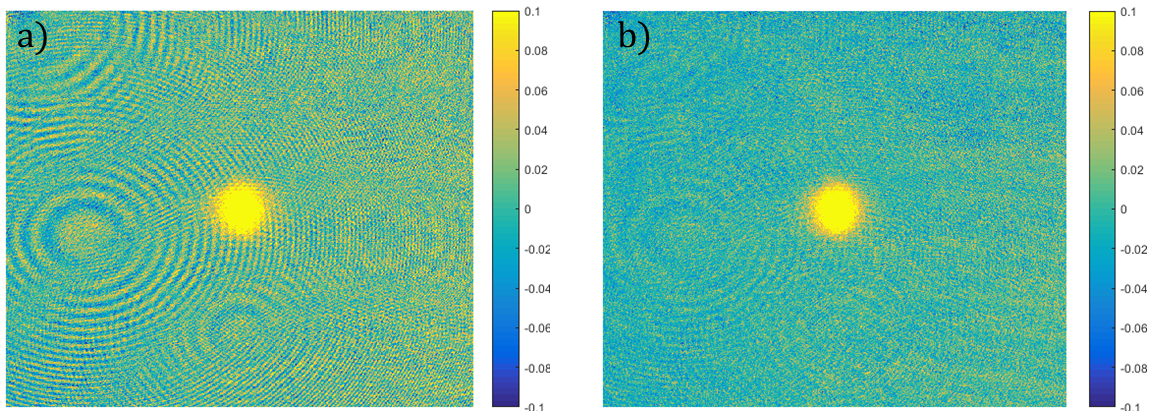
\includegraphics[width=\textwidth]{misc_PCAcomp.png}}
		\caption{Comparison of background subtraction methods}{Background subtraction on the same image performed using two different methods and plotted on the same color scale. a) The partner-in-time background to the atom image is used. b) A composite background image formed via PCA is used.}
		 \label{fig:PCAcomp}
	\end{figure}
While PCA does not completely eliminate the visible fringe patterns, there is a noticeable reduction of the fringes in the PCA image versus the partner-in-time method.

\subsubsection{Highly tunable 689\,nm spectroscopy system}
The spectroscopy laser is derived from a dedicated slave diode and is our primary 689\,nm probe for bosonic isotopes, with the spin manipulation laser described below being used for fermions.
This laser system is used for general intercombination line spectroscopy, photoassociation, Bragg scattering, and Rabi oscillation measurements.

Fig.\,\ref{fig:689specSch} shows a simplified optical diagram.
	\begin{figure}
	\centerline{
		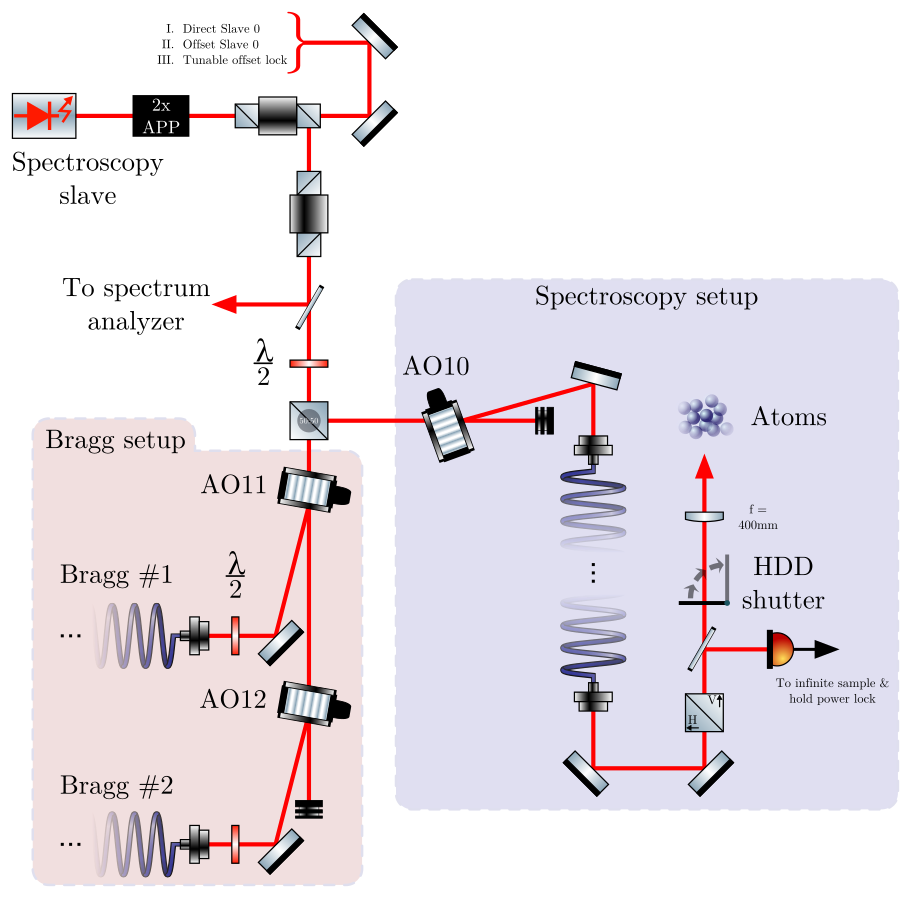
\includegraphics[width=\textwidth]{689_specSlaveSchematic.png}}
		\caption{Optical schematic: 689 spectroscopy laser}
		 \label{fig:689specSch}
	\end{figure}
We found it necessary to increase the isolation out of the laser as the injection lock became unstable when coupling into the fiber couplers due to back reflections.
We typically get $\sim25$\,mW of usable power past the second isolator.
As this is our primary spectroscopy laser, its optical setup tends to be in flux but a couple of noteworthy innovations have been implemented in recent years.
These include the development of an infinite sample and hold for intensity stabilization, a versatile injection locking scheme, and a shallow angle Bragg scattering setup.

The infinite sample and hold (ISH) circuit is used in conjunction with an intensity stabilization lock circuit and was built to allow for intensity stabilized "chirped" pulses on timescales much faster then the acquisition time of the intensity lock circuitry, typically $\sim70$\,ms.
This circuit was developed and built by Josh Hill and is based on the LTC1417 which is a low power 14-bit 400\,kS/s ADC.
Details of the circuit construction and characterization are left to Josh's forthcoming thesis.
The ISH is currently placed on our spectroscopy probe and is situated between the intensity stabilization lock circuit and RF voltage controlled attenuator.
This allows the ISH to passively sample the control voltage from the lock circuit.
In sample mode the ISH output follows the input from the lock circuit.
When the ISH is transitioned into hold mode, it begins ignoring changes on its input and outputs the last voltage that was sampled before the transition.
A timing disgram of the infinite sample and hold usage is outlined in Fig.\,\ref{fig:689specInfSH}.
	\begin{figure}
	\centerline{
		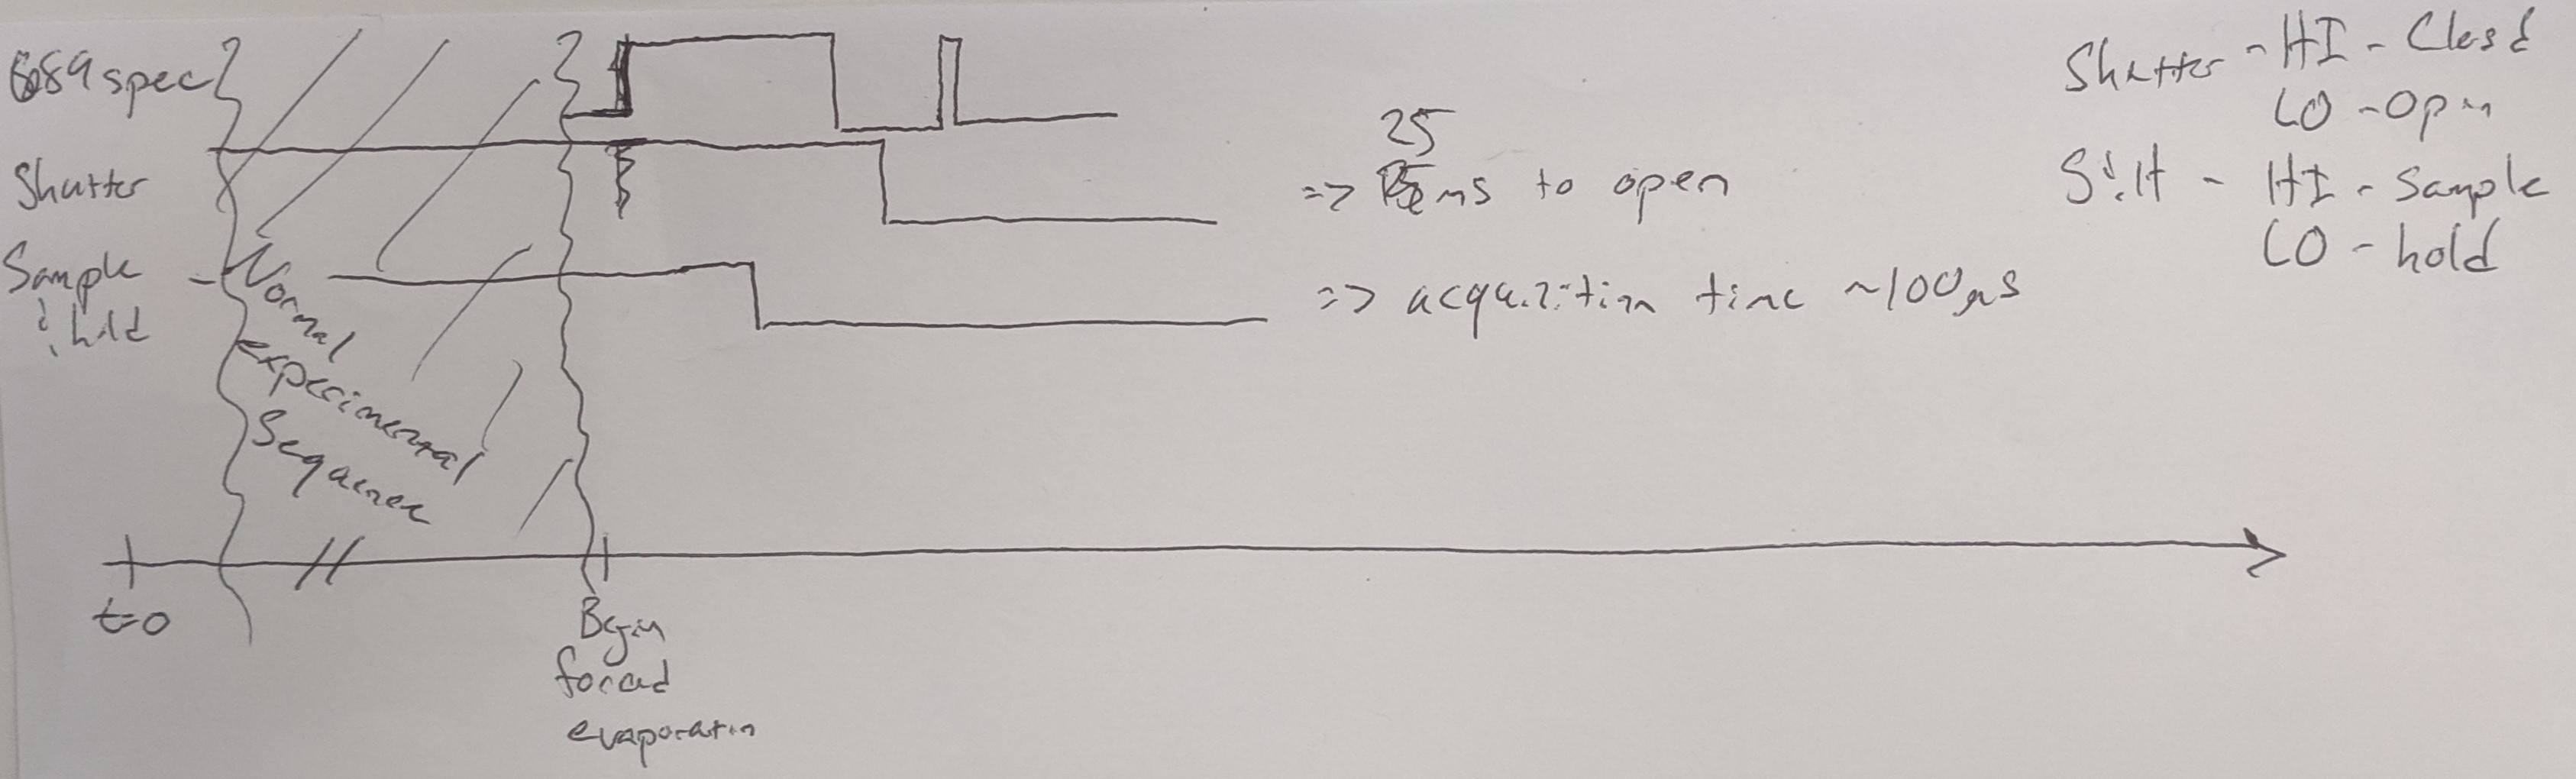
\includegraphics[width=\textwidth]{689_specInfSH.jpg}}
		\caption{Infinite sample and holding timing diagram}{The HDD shutter in use has a full open time of $\sim15$\,ms and the acquisition time of the sample and hold chip is on the order of $\sim500ns$.}
		 \label{fig:689specInfSH}
	\end{figure}
Following our typical preparation sequence we place the ISH in sample mode and enable the spectroscopy probe with the HDD shutter blocking the beam. 
This allows the lock circuit time needed to acquire and stabilize the feedback voltage required to maintain the current intensity setpoint.
Following lock acquisition, we transition the ISH into hold mode, open the shutter, and pulse the RF onto the spectroscopy AOM (AO10) via a fast RF switch (model: Mini-circuits ZASWA-2-50DR+) where the RF amplitude is attenuated via a voltage controlled attenuator and the voltage input is the fixed output value from the ISH.
This momentary transition to open-loop operation of the intensity stabilization circuit does suffer from slow long term fluctuations shot to shot, but does provide a marked improvement on the intensity reproducibility without placing restrictions on the minimum pulse time required.
Furthermore, by monitoring and recording the slowly varying intensity fluctuations, we can model any error introduced by the reduced intensity variation.

Another notable improvement has been the versatile injection locking scheme for varying the frequency of the spectroscopy slave with respect to the maser laser.
This scheme allows us to change the seed laser frequency via three different methods outlined below.
\begin{outline}[enumerate]
	\1 Directly following slave 0
		\2 A small amount of light from slave 0 is coupled directly into the rejected port of the spectroscopy slave, resulting in the frequency of spectroscopy slave and slave 1 being shared. 
		Fig.\,\hl{something} shows the position of this pick-off before the boson red MOT AOM. 
		Recalling that slave 0 is always positioned +82\,MHz of the bosonic isotope of interest, the direct method will position the frequency of the spec. slave to also be +82\,MHz.
	\1 Slave 0 minus 40\,MHz
		\2 The light sent from slave 0 is shifted down 40\,MHz by the spec. offset AOM. This positions the spec. slave frequency at +42\,MHz of the intercombination line of interest.
	\1 Programmable offset
		\2 In 2018 we re-purposed the original homemade 689 master ECDL described in Natali's thesis as a slave ECDL and directed light from this setup as a tertiary method for tuning the frequency of the spec. slave. 
\end{outline}
There are several things to note concerning the above descriptions.
First, to reiterate, the "of interest" designation specifically refers to the variability of the laser frequency of slave 0 which is dependent on the configuration of the isotope selector AOM as discussed in Sec. \hl{somewhere}.
Second, switching between case I and II is surprisingly trivial given the realized setup on the table.
In practice, a flipper mirror and clever optical path alignment allow us to switch between these two injection methods in a matter of seconds and has demonstrated remarkable stability.
Thirdly, while the programmable offset is the most versatile of the presented schemes, it also has the greatest frequency uncertainty and is fundamentally a different approach that we are still in the process of exploring.

The slave ECDL, beatnote generation, and phase locked loop (PLL) integrated circuit was a project begun by a visited student and later completed by Josh Hill.
We will leave the detailed description of the Neutral implementation for Josh's forthcoming thesis and instead reserve our current discussion to an overview of the technique.
It is based on the 2009 work of Appel et. al. \cite{zfr08expansion} which outlines a versatile optical phase locked loop with a claimed frequency range of sub-MHz to 7\,GHz.

As a brief reminder, phase locking is a feedback scheme which seeks to maintain the frequency difference between two sources.
This process is heavily used in the telecommunications industry and analog phase locking is a common technique in atomic physics laboratories as well.
In atomic physics, the general idea is to generate a beatnote by interfering two single frequency lasers on a high bandwidth photodiode.
From this optical beatnote we intrinsically observe the difference frequency of the two lasers as the summing frequency is well outside the bandwidth of photodiodes.
The difference frequency can then be further interfered against an RF reference frequency and low-passed to generate an error signal which can be used to stabilize the difference frequency against the RF reference.

The versatile OPLL is a digital realization of this approach which we have used to lock the relative frequency difference between the Toptica master and slave ECDL from approx. 1\,MHz to 1.2\,GHz.
The upper limited is currently bandwidth limited by our AC coupled photodiode and not by the OPLL circuitry.
Fig.\,\ref{fig:offsetDetails}a) shows an example of the optical beatnote monitored via an RF spectrum analyzer.
Notably, while we do observe suppression of frequency components around the set point which is characteristic of locking, we also see resonant peaking instead of a single narrow frequency peak as expected.
Further investigations showed that the individual frequencies were fairly narrow as shown in Fig.\,\ref{fig:offsetDetails}b) where we observed atom loss on the $F=9/2\,\rightarrow\,F=11/2$ transition with linewidths on the order of 60\,kHz.
	\begin{figure}
	\centerline{
		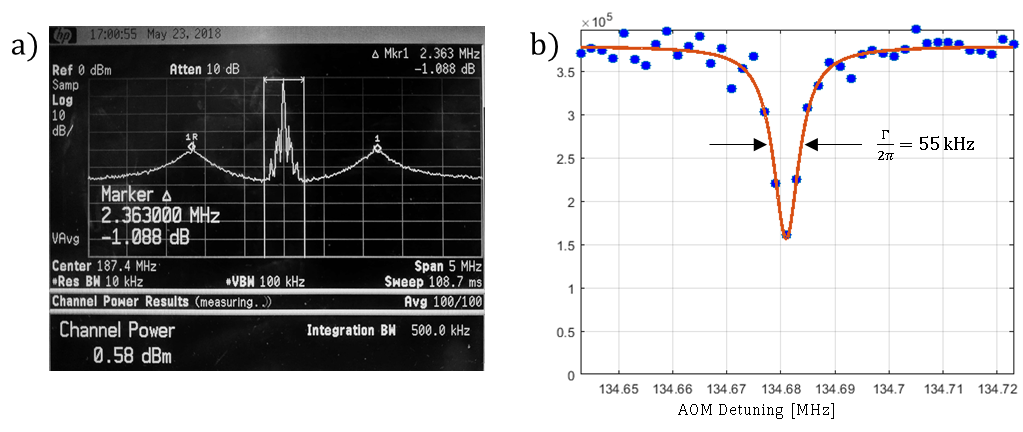
\includegraphics[width=\textwidth]{689_offsetLockCharacterization.png}}
		\caption{Characterization of the OPLL performance}{a) RF spectrum of the optical beatnote when the OPLL is engaged. Resonant peaking can be seen in the 500\,kHz band around the center frequency. b) Atom loss spectrum which shows that the resonant features are at discrete frequencies. Differences between the AOM detuning shown and the center frequency of the OPLL are due to various AOM shifts between components.}
		 \label{fig:offsetDetails}
	\end{figure}

Finally, we note that this system has also been used to perform Bragg spectroscopy as reported in the PhD thesis of Brian DeSalvo.
Detailed drawings of the optical setup used for shallow angle Bragg scattering can be found in App. \hl{something}.


\subsubsection{Spin-manipulation laser with dynamic polarization control}
Fermionic strontium 87 has become of major interest for experiments studying quantum magnetism in a highly degenerate SU(N) system. \hl{rephrease}.
Key to these studies is the creation and manipulation of arbitrary spin mixtures.
We have recently implemented a spin manipulation laser probe (spin-man) acting on the $F=9/2\,\rightarrow\,F=11/2$ hyperfine transition of the intercombination transition for the purpose of creating well defined spin mixtures.
Preliminary investigations using this system are reported in Ch. \ref{ch:chap6}.

Fig.\hl{something} highlights a simplified optical schematic of the spin-man system which is derived from slave 1 and is related to the stir MOT system outlined above in Sec. \hl{something}.
The original construction of the output optics is outlined in Ch. 5 of Josh Hill's masters work \cite{Hill2017} and is part of the layered optical systems added to the top of the optical chamber in 2017.

A major component of this layered system is the liquid crystal retarder (model: MeadowLark Optics LV-300 LCR) which allows us to dynamically control the polarization incident on the atoms.
Additionally, a configurable high precision RF system for dynamically changing the spin-man laser frequency has allowed us to demonstrate optical pumping in a magnetic field using $\sigma+$ light where we can individual address each sub-level transition independently.
Once we have spin polarized the gas, the LCR can flip the light polarization and probe the polarized ground state along the $^1S_0\,(F=9/2,m_F=9/2)\,\rightarrow\,^3P_1\,(F=9/2,m_F=7/2)$ using $\sigma-$.
Details of these experiments and further characterization of this system are presented in Ch. \ref{ch:chap6}. 

The RF tunability for optical pumping is based on the "table mode" feature of the Novatech 409B digital synthesizers which can be externally triggered to progress through a table of configured frequencies.
These synthesizers are discussed in greater detail in \hl{somewhere}.

\section{Apparatus interface} \label{sec:electronics}
\setcounter{footnote}{0}
The Neutral apparatus interfaces to our digital infrastructure via a plenitude of specialized hardware implementations and custom written software.
Over the last seven years nearly all of this digital infrastructure has been refactored, upgraded, or replaced.
Therefore, the following sections will briefly outline these new constructs, providing references to code repositories when possible.
However, detailed discussions on the usage of this infrastructure will be relegated to their respective appendices.

\subsection{Software} \label{ssec:soft_sys}
The primary control software is a custom built Labview application based on a synchronous state machine\footnote{Currently this project can be found at \texttt{https://github.com/KillianRice/neuKlein}}\hl{ref}.
The Neutral implementation of this software is called neuKLEIN (Neutral Killian Lab Experimental Interface) and is based on a major overhaul, by Joe Whalen, of the original control software.
A detailed overview of the capabilities, limitations, and instructions for use of neuKLEIN is available in App. \ref{app:neuKLEIN}.

In short, an experimental sequence begins with serially programming each voltage output device.
The pulseblasters are programmed last and are triggered via the global experimental trigger discussed in \ref{sec:expTrig} below.
Once all devices are ready the pulseblasters become the global clock and the neuKLEIN software begins polling the PixelFly camera waiting for a new image.
Once an image is received various experimental parameters are recorded into text files and saved to disk.
This process continues within the primary WHILE loop of the state machine and steps through the predetermined experimental settings array.
Primary exit conditions for the loop are encountering an error, conclusion of the settings array, or manual abortion.

Once the files are written to disk, we perform image analysis using a custom Matlab$^{TM}$ routine imaginatively named Neutral imagefit routine\footnote{Currently this project can be found at \texttt{https://github.com/KillianRice/neutral\_imagefit\_routine}}.
An in-depth discussion on the usage, extensibility, limitations, and feature improvements is available in App.\,\ref{app:imagefitManual}.

\subsection{Hardware control and measurement systems} \label{ssec:comp_sys}
The hardware control system is composed of several primary components including the experimental clock, voltage output devices, and measurement instruments.
We use a series of National Instruments$^{TM}$ data acquisition cards (NI-DAQs) and a reconfigurable FPGA for generating output voltages.
The experimental clock is based on a pair of SpinCore PulseBlaster TTL generators and a Cooke PixelFly camera is used for collecting absorption images.
We also have access to a PicoScope 5000 digital oscilloscope for high resolution signal monitoring and recording. Typically this is used for recording experiment specific photodiode signals for later analysis.

\begin{table}[]
\centerline{
\begin{tabular}{@{}|c|cc|c|cc|@{}}
\toprule
\multirow{2}{*}{Model} & \multicolumn{2}{c|}{Resolution} & \multirow{2}{*}{\begin{tabular}[c]{@{}c@{}}FIFO\\ buffer Size\end{tabular}} & \multicolumn{2}{c|}{Max sample rate} \\ \cmidrule(lr){2-3} \cmidrule(l){5-6} 
 & Bit depth & Voltage {[}mV{]} &  & Channels used & Rate {[}kS/s{]} \\ \midrule
\multirow{4}{*}{6713} & \multirow{4}{*}{12} & \multirow{4}{*}{5} & \multirow{4}{*}{16,384} & 1 - 5 & 1,000 \\
 &  &  &  & 6 & 952 \\
 &  &  &  & 7 & 833 \\
 &  &  &  & 8 & 740 \\ \midrule
\multirow{2}{*}{6221} & \multirow{2}{*}{16} & \multirow{2}{*}{0.03} & \multirow{2}{*}{8,191} & 1 & 833 \\
 &  &  &  & 2 & 740 \\ \midrule
\multirow{4}{*}{6229} & \multirow{4}{*}{16} & \multirow{4}{*}{0.03} & \multirow{4}{*}{8,191} & 1 & 833 \\
 &  &  &  & 2 & 740 \\
 &  &  &  & 3 & 666 \\
 &  &  &  & 4 & 625 \\ \midrule
\multirow{4}{*}{6733} & \multirow{4}{*}{16} & \multirow{4}{*}{0.03} & \multirow{4}{*}{16,384} & 1 - 5 & 1,000 \\
 &  &  &  & 6 & 952 \\
 &  &  &  & 7 & 869 \\
 &  &  &  & 8 & 769 \\ \bottomrule
\end{tabular}}
\caption{Arbitrary waveform generation details}{All cards specified are the PCI model and interface with the experiment control computer directly through the motherboard or via a PCI expansion bin (model: StarTech PEX2PCIE4L). Sample rates are given in kilosample per second (kS/s) and is the same across all enabled channels. The FIFO buffer stores the individual waveform points and is also shared amongst all enabled channels. Full voltage output range is $\pm$10\,V.}
\label{tab:niDaqs}
\end{table}
Table \ref{tab:niDaqs} gives the models of the NI-DAQ cards and additional details such as the resolution, the shared FIFO (first-in, first out) buffer sizes, and the maximum sample rates as a function of the number of channels in use.
Though these cards are known as acquisition cards, we instead rely heavily on the arbitrary waveform generation capabilities for dynamically generating analog output voltages.
Furthermore, we do not stream data to cards during the experimental sequence but use only the on-board FIFO buffer for storing the arbitrary waveform.

It is important to remember that the finite buffer size and maximum sample rate define two extremes for time based waveform generation due to the discretization of the waveform.
For short times, the maximum sample rate sets the minimum possible time step between two points on the voltage output.
At long times, a fixed number of points between the start and end points may lead to unacceptably large voltage steps between two points on the voltage output.
Balancing these two tradeoffs is essential and is the primary driver for the plethora of various cards so that we may dedicate their finite resources to specific tasks.

While arbitrary waveform generation is useful for dynamically varying voltages during an experimental sequence, there are a number of applications where a static voltage is needed or smoothly varying between two or more voltages is not required.
Until recently, the NI-6713 was our only sources of experimentally controlled static voltages (in contrast to a static voltage from a supply) and switching between driving voltages was done via a bank of standalone fast analog IC switches (primarily the ADG419).
Fast switching of the set point voltage has traditionally been how we control a number of systems through their feedback circuitry.
For example, the 922\,nm frequency is jumped from the optimal trapping frequency to the optimal imaging frequency at the end of the experimental sequence via the sat. abs. solenoid current.
The change in magnetic field shifts the resonance frequency of the loss feature and the 922\,nm frequency lock responds by varying the master laser frequency to restore the resonance condition.
Therefore, while imperative to retain this functionality, the NI-6713\,$+$\,switch bank limited in the number of controlled static voltages to eight and the simple standalone switches were insufficient for applying application logic for dynamically choosing driving voltages\footnote{An example of this application logic might be any set point which could be controlled via boolean logic conditioning.}.

These shortcomings led us to develop a real-time based NI-FPGA for the development of custom reconfigurable logic and static voltage output.
This system is based on a NI cRIO-9063 with integrated Artix-7 FPGA, a NI-9403 32ch TTL input/output (I/O) module, and a NI-9264 16ch analog output module.
The cRIO device manages the control layer of the system, hosting the embedded operating system and allows us to easily develop, compile, and deploy our custom control logic to the FPGA via Labview.
The FPGA (field programmable gate array) executes the user-defined logic on a user-defined loop-time (minimum 50\,$\mu$s.) with the 32 TTL I/O channels and 16 analog output available for reading and writing each cycle.
We typically do not use the output functionality of the TTL channels and instead opt for 32 input channels which can be dynamically assigned to control the 16 analog outputs.
These analog outputs may be conditioned as static, simple switched, cascading switched, or simple boolean controlled outputs all configurable via software.
Additional features include logic inputs which can be shared to multiple outputs and simple waveform generation such as linear ramps.
Detailed schematics of the input/output conditioning circuits as well as limitations, capabilities, and usage instructions are available in App. \hl{somethign}.

\subsection{Ancillary laboratory systems} \label{ssec:misc_sys}
\subsubsection{MOT coils}
The Neutral MOT coils are a complementary pair of custom made high aspect ratio solenoids which, in an anti-helmholtz configuration, can generate magnetic field gradients on the order of 150\,G/cm.
Fig.\,\ref{fig:motCoilField} shows the on-axis magnetic field.
In the center of the chamber, along the Z axis, the field gradient varies with current as 19.1\,(G/cm)/A.
	\begin{figure}
		\centerline{
		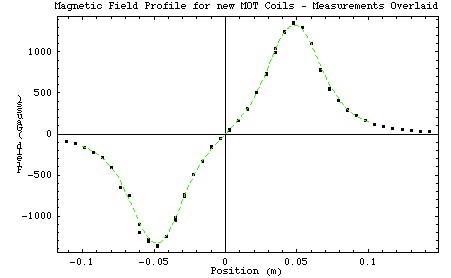
\includegraphics[width=0.75\textwidth]{misc_MOT_B_Field Profile.jpg}}
		\caption{MOT coil on-axis magnetic field}{The expected and measured B-field along the Z-axis. The measured field gradient calibration is 19.1\,(G/cm)/A}
		\label{fig:motCoilField}
	\end{figure}

\subparagraph{Historical:}
\setcounter{footnote}{0}
MOT coils were wrapped by Natali and Pascal in June of 2004.
They are wrapped using \hl{something} hollow core wire which is water cooled.
The current source in use is a \hl{something} which uses a high power FET switch to drop current across the coils.
A custom-built high-precision low resistance current sensing configuration monitors this current to actively feedback and maintain constant current through the coils \footnote{Further information and detailed notes on the wrapping can be found in \texttt{KillianDrobo:\textbackslash\textbackslash Neutral\textbackslash Laboratory Systems\textbackslash MOT Coils}}.

%\subparagraph{Potential improvement:}
%Currently the Neutral apparatus uses the same coils and supply for both the blue and red MOTs.
%However, due to the $S=1$ of the triplet system, the Zeeman shift is significantly stronger for the $^3P_1$ state. \hl{check this reasoning, the different is 1.4 MHz/G vs 2.1 MHz/G so can't be only factor}
%Consequently, we need much less current running in the MOT coils for red MOT operation.
%The blue MOT utilizes approx. 42\,Amps ($\sim$ 76\,G/cm) while the red MOT needs on the order of 100\,mAmps ($\sim 2$\,G/cm).
%These small currents for the red MOT are observed to be near the noise floor of the circuit.
%For this reason the Rydberg apparatus implemented separate red and blue MOT coils.
%We have investigated wrapping a new set of coils to follow this example but have not found a feasible to solution.
%Alternatively, we have discussed changing out the current supply dynamically between MOT operation using an H-bridge configuration as discussed in Melissa Revelle's thesis \hl{ref}.
%We have not currently pursued this option at this time.

\subsubsection{Trim coils}
Cubic trim coil cage (\hl{size?}) with the coils in a Helmholtz configuration.
These coils are used to trim out static residual B-fields and to apply dynamic and well controlled external magnetic fields.
We commonly use the coils along the Z-direction to apply bias magnetic fields during spectroscopy as shown in Fig.\,\ref{fig:trimField}a).
	\begin{figure}
		\centerline{
		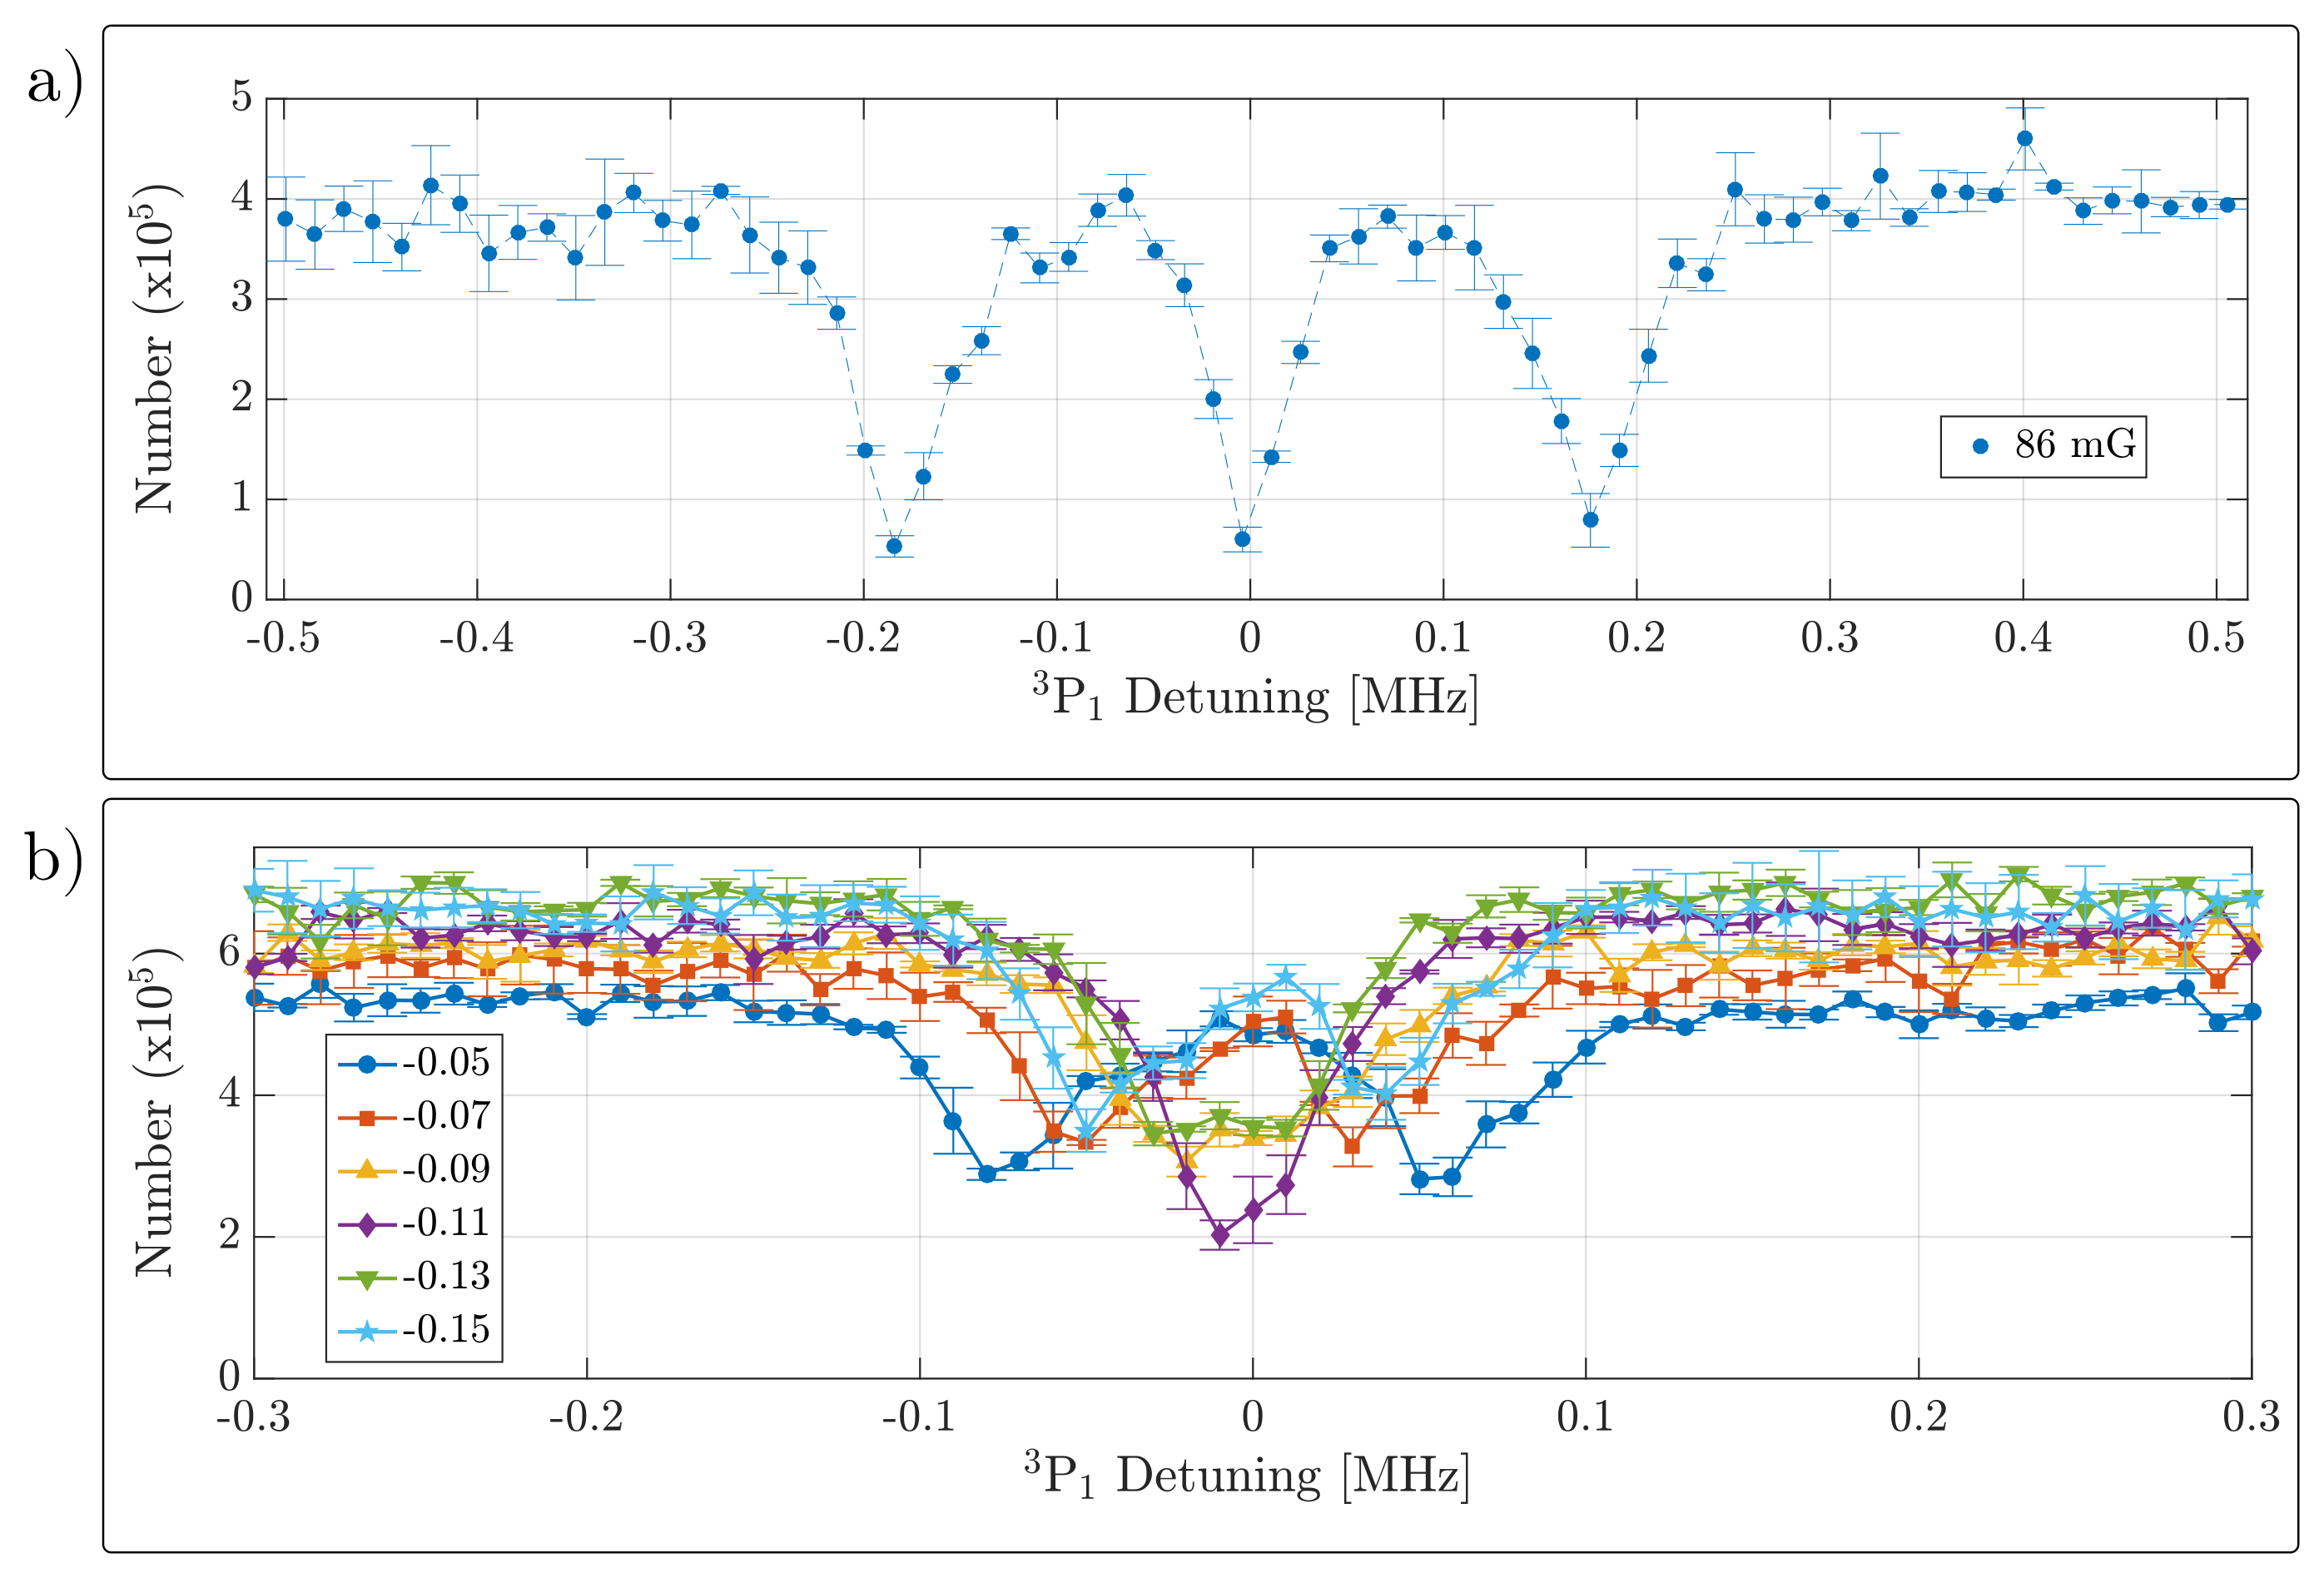
\includegraphics[width=\textwidth]{misc_trimField.png}}
		\caption{Zeroing residual magnetic fields}{Loss spectroscopy in various bias fields. a) Example of resolved Zeeman splitting of the $^3P_1$ magnetic sub-levels. b) Typical B field variation for determining the zero field position. The applied bias is increased for each subsequent scan and a clear zero crossing is observed. The legend has been left in arbitrary lab units to emphasis the B-field zero crossing which occurs around -0.11.}
		\label{fig:trimField}
	\end{figure} 
	
The fine-structure magnetic sub-levels of the $^3P_1$ state vary with B-field as 2.1\,MHz/G.
Compared to the natural linewidth of 7.5\,kHz, this splitting of the $^3P_1$ states provides a very sensitive probe for precisely zeroing the residual magnetic field.
We determine the required bias fields by performing loss spectroscopy with unpolarized light along the $^1S_0\,\rightarrow\,^3P_1$ transition using a bosonic isotope.
Next we fit the $m_j=\pm1$ spectral features to a loss line-shape (either gaussian or lorentzian) and plot the line center as a function of applied magnetic field along each dimension.
Fig.\,\ref{fig:trimField}b) shows an example of the change in Zeeman splitting of the m$_j$ levels using strontium-84.
Finally, we perform a linear fit to the line center variation and extract the intercept which nulls the residual field and the slope which calibrates our applicable field strength per ampere. 
We have found these calibrations to be [$\delta B_z = 0.985, \delta B_y = 0.982, \delta B_z = 0.987$]\,G/A\footnote{Further details available in Onenote under Research Projects $\rightarrow$ Routine Studies $\rightarrow$ B-field zeroing $\rightarrow$ Zeroing summary}.

\subsubsection{Zero crossing AC line trigger} \label{sec:expTrig}
Fig.\,\ref{fig:zeroCrossTrig} shows the circuit used to start the Neutral experimental sequence.
	\begin{figure}
		\centerline{
		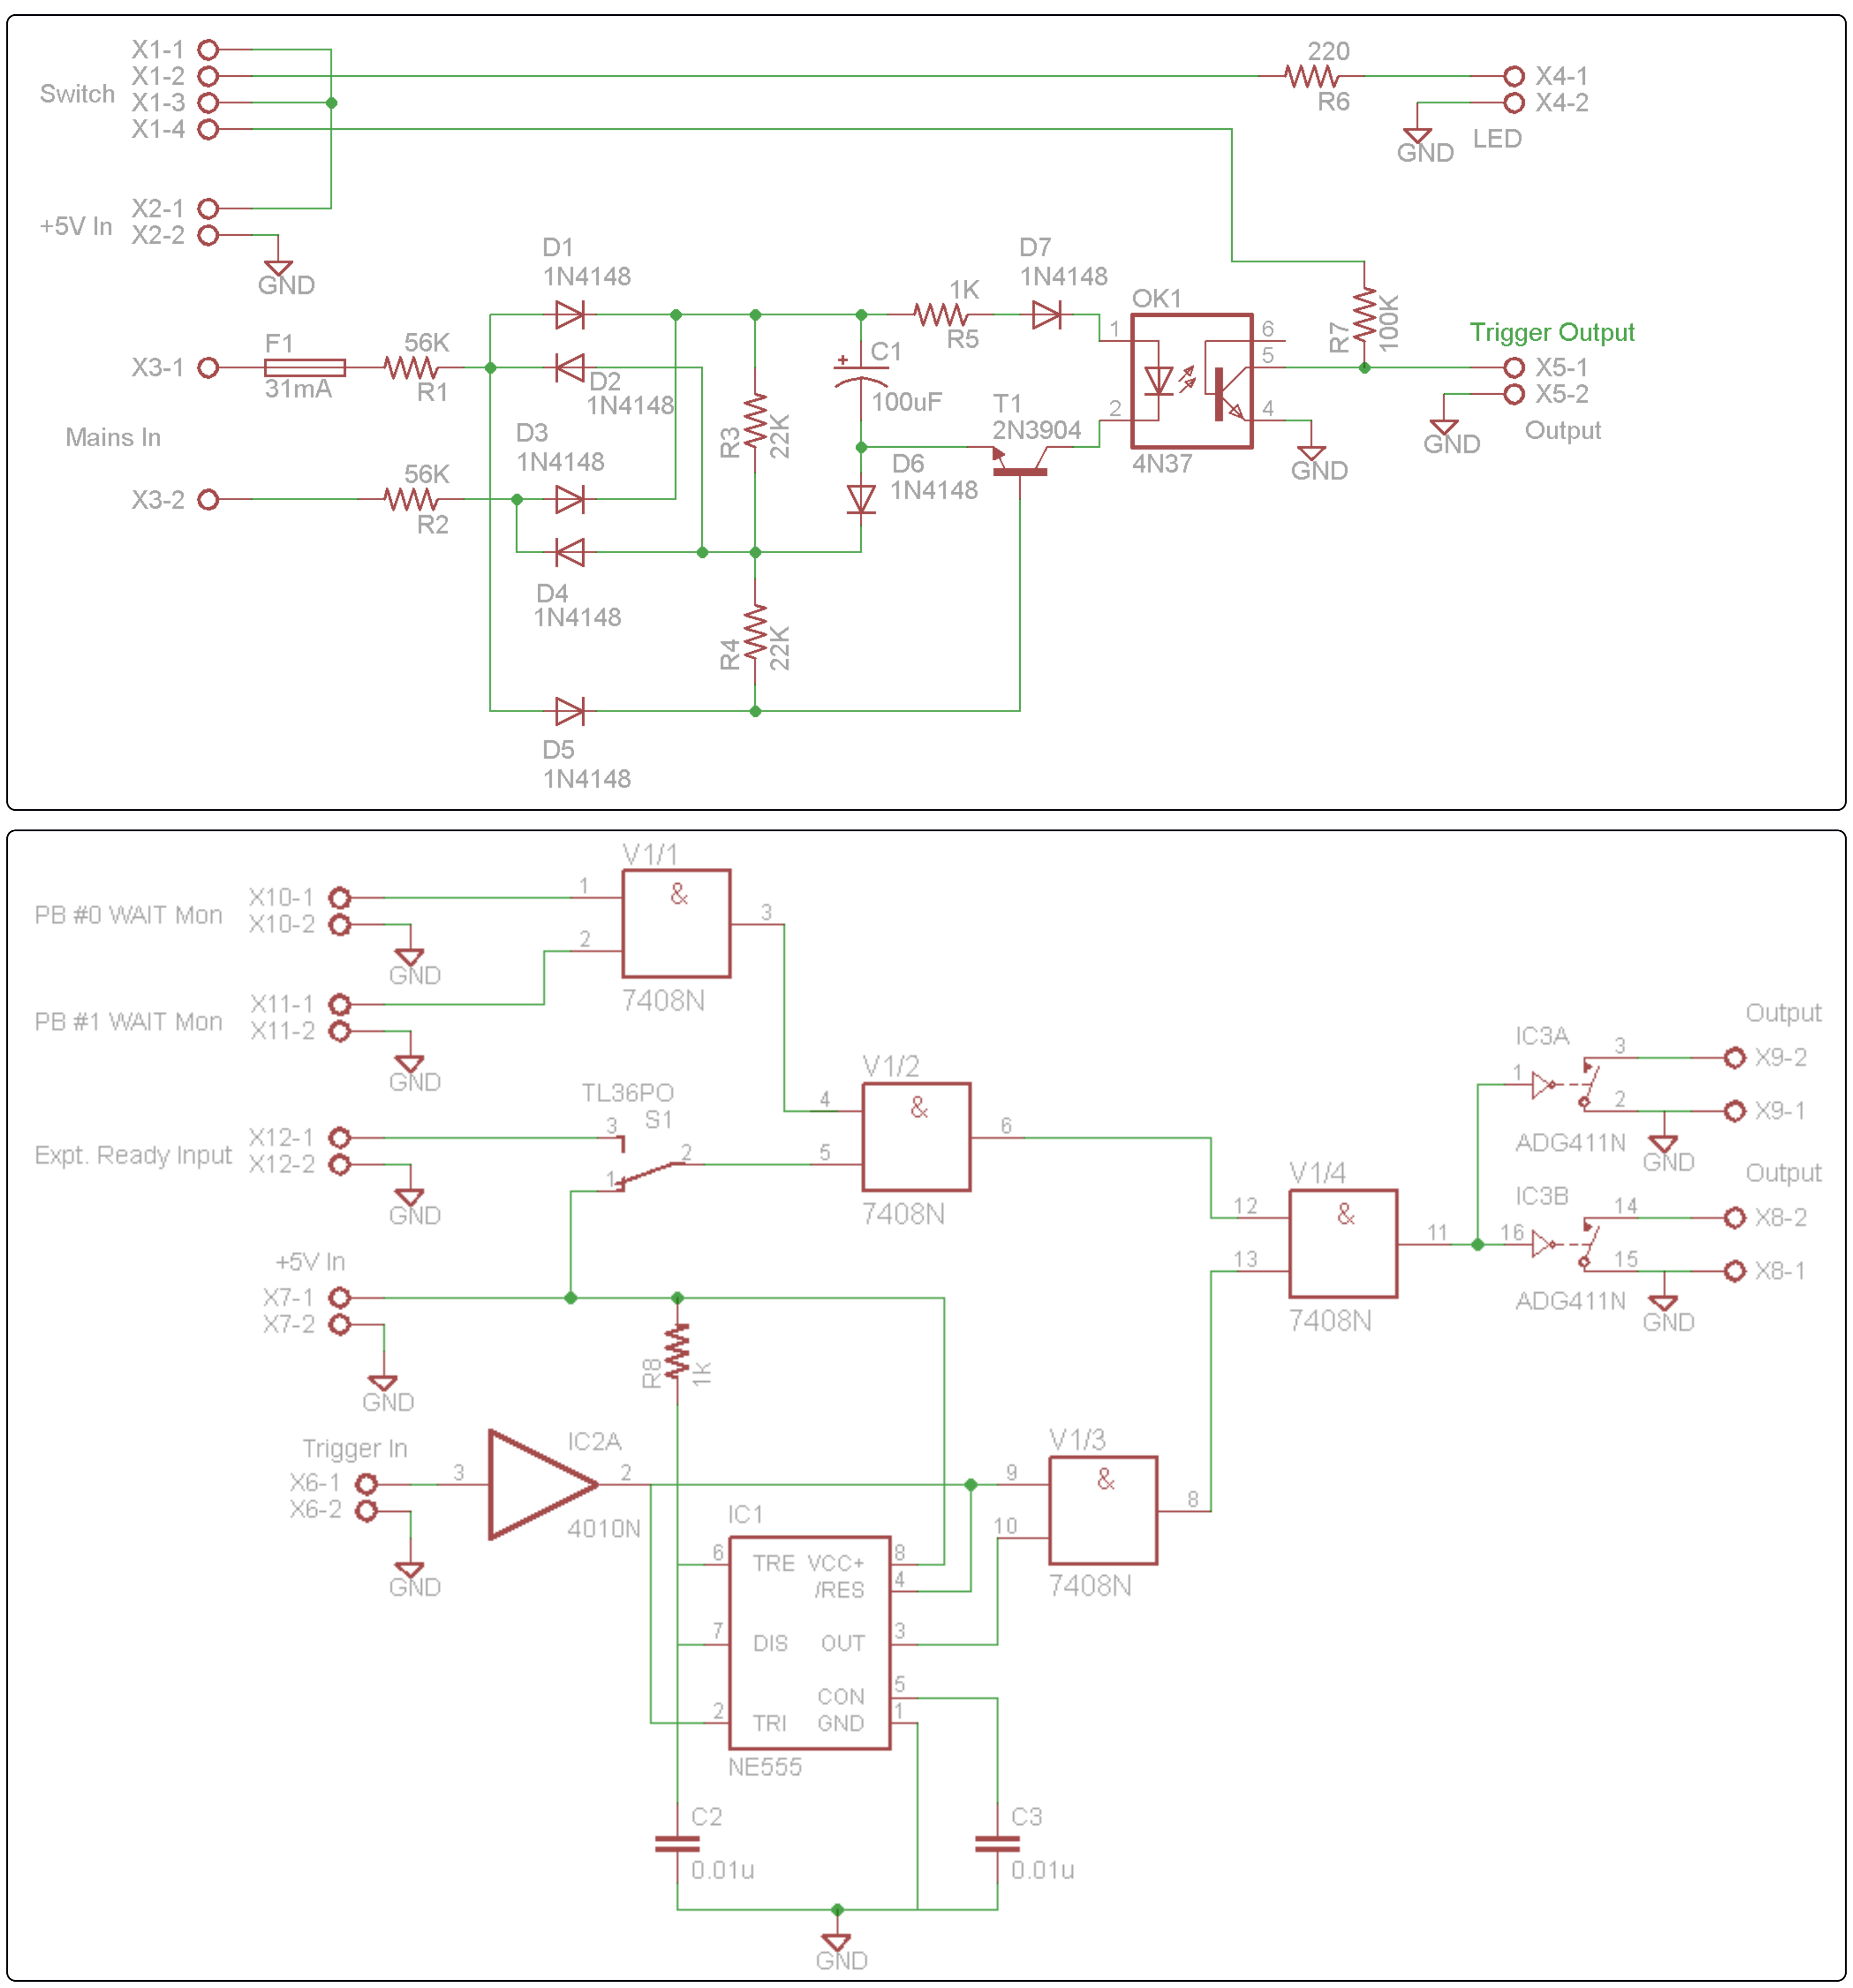
\includegraphics[width=\textwidth]{misc_acZeroCrossingSyncTrigger.png}}
		\caption{Circuit diagram of the zero crossing AC line trigger}{Top - 120\,Hz square wave pulser which generates a short pulse on the 60\,Hz zero crossing. Bottom - Synchronizer circuit between both pulseblasters, an optional expt. ready trigger (which ensures the atom shutter is open), and the AC zero-crossing trigger. Trigger input is from the top circuit and is used with the 555 timer in a one-shot configuration. This ensures only every other pulse from the AC trigger produces a HI output past the AND gate V1/3.}
		\label{fig:zeroCrossTrig}
	\end{figure} 
It is based on deriving a TTL pulse at the positive-going zero crossing of the 60\,Hz building line.
Manual triggering is essential since we do not share the same clock source between the two independent pulseblasters (PB0\,\&\,PB1).
Instead relying on their relative precision and low timing jitter to maintain experimental synchronicity when triggered from a shared source.
Fig.\,\ref{pbTimingJitter} shows a comparison of the timing uncertainty when a short 200\,ns pulse is output from both pulseblasters and the oscilloscope is triggered from the zero crossing of the AC line.
	\begin{figure}
		\centerline{
		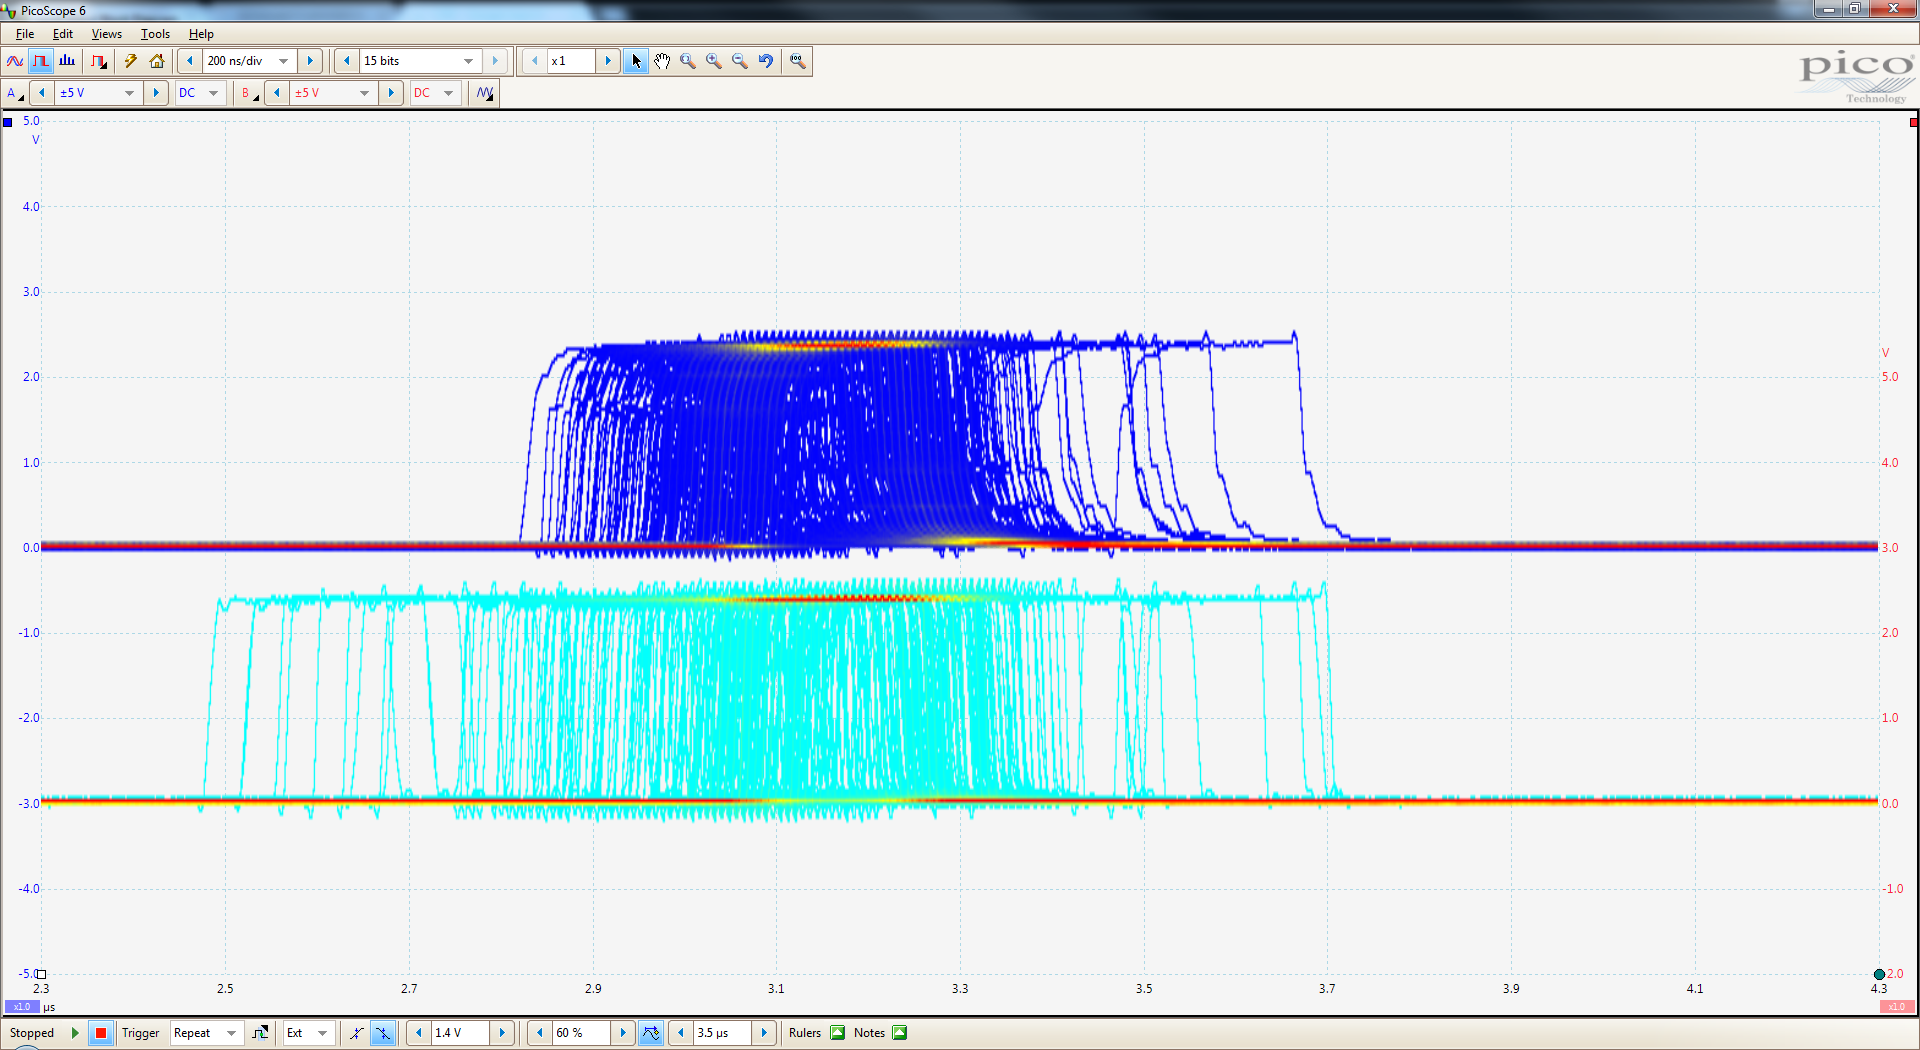
\includegraphics[width=\textwidth]{misc_PB_TriggerJitter.png}}
		\caption{Comparison of pulseblaster timing jitter}{A persistent oscilloscope trace showing repeated measurements of a 200\,ns logic pulse from each pulseblaster. The upper signal is PB0 and the lower is PB1. The scope is externally triggered by the zero crossing AC line trigger.}
		\label{fig:pbTimingJitter}
	\end{figure} 
While this measurement does not reveal the cause of the relative instability between the three sources (PB0, PB1, or AC line), we do observe a relative instability of approx. 1\,$\mu$s.
For most use cases with ultracold matter, this timing uncertainty is entirely reasonable and presents no practical limitation.
However, this behavior does preclude the usage of cross-triggers between the pulseblasters when performing experiments with the optical lattice\footnote{Cross-triggers are defined as the mixing of timing signals between the two pulseblasters.
For instance, using PB0 to trigger the turn on of lattice arm A and PB1 to trigger arm B.}.
This timing difference results in a similar consideration as the discrete timing issue discussed previously whereby, dependent on the dynamics under investigation, even small timing difference can lead to significant variation in the observed phenomena.
We mitigate this effect by taking care to trigger all related processes from the same pulseblaster where the timing jitter is reduced to 50\,ns.

We choose to trigger off the building wide 60\,Hz line in order to maintain a fixed phase relationship from shot to shot.
This is thought to act as a common-mode rejection of electrical noise which could couple into our measurements via intensity or frequency noise.
However, we have not rigorously evaluated this hypothesis and no significant change was observed when changing the global experimental trigger.

Finally, the additional logic gates ensure that the pulseblasters trigger at the same time since they are programmed serially by the neuKLEIN software.
This process is enabled by a WAIT signal that each pulseblaster outputs when in this state which is used to ensure proper initialization of the system before starting an experimental sequence.

\subsubsection{Pneumatic actuated mirror mounts}
One challenge of using a 532\,nm optical lattice is that this wavelength is between the 461\,nm and 689\,nm wavelengths used for our MOT beams and the 532\,nm must operate at high power.
For the lattice arms in the plane of the atoms (A \& B) we combine and separate the lattice light along the 1064\,nm ODT path using common harmonic beamsplitters.
However, the vertical path (arm C) presents a significant challenge as the numerical aperture along this path into the chamber is restricted by the MOT coils.
Moreover, maintaining clean polarization of the MOT beams requires us to place the MOT waveplate along the vertical axis so as to avoid mirror reflections which may rotate the polarization.
This places prohibitive constraints on the availability of passive optical components which might combine the MOT and lattice traps.
Currently, we employ industrial pneumatic valves (model: \hl{model}) with actuators (model: \hl{moel}) to move the waveplates and requisite MOT mirrors out of the path before turning on the 532\,nm light.
Fig.\,\ref{fig:pnuSys} shows the flow diagram for switches S1 and S2 for this system.
	\begin{figure}
		\centerline{
		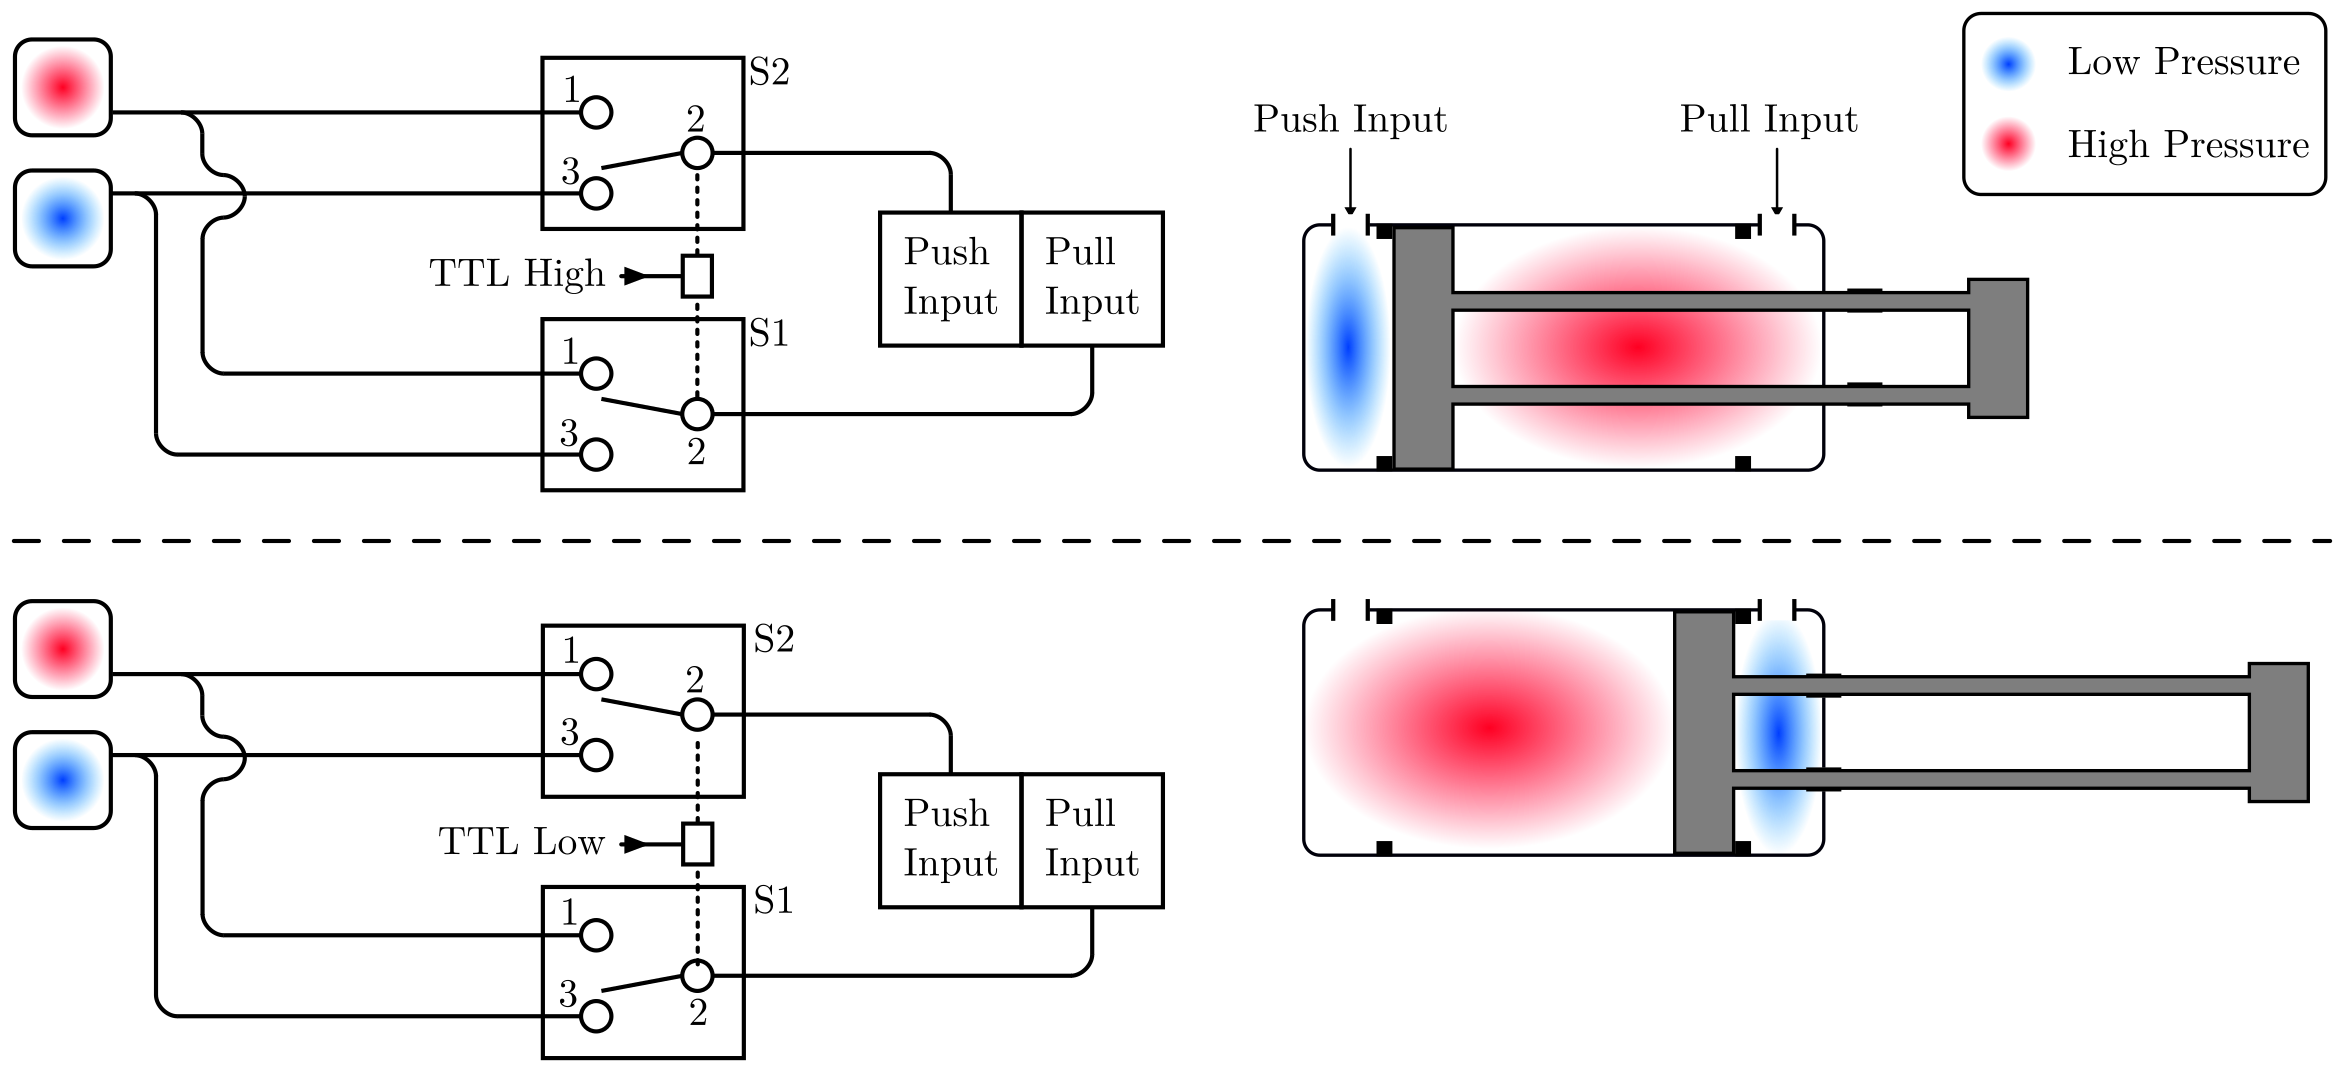
\includegraphics[width=\textwidth]{misc_pneumaticSystem.png}}
		\caption{Pneumatic actuators diagram}{Example schematic for a single actuator. Three actuators are used on the apparatus to move several components simultaneously. Not shown is the 4-way cross which splits the output from each valve (S1 and S2) to each actuator.}
		\label{fig:pnuSys}
	\end{figure}
As one might expect, this abrupt movement does impart vibrations into to the table which we dampen by slowing the movement and cushioning the stops.
In practice we find that the system is fairly robust against these small "kicks" though occasionally the air pressure must be adjusted if the lasers are behaving erratically..
We have also observed a settling of the actuators when extended as this is this default position.
Future improvements may aim to provide a rail system for guiding the movement and supporting the actuators against gravity for smoother movement.
\chapter{Photoassociation in ultracold gases}
\label{ch:chap3}

\section{Introduction}
\label{sec:pas_intro}

% Intro
This part needs to be brief and really should motivate the idea of PAS.

PA is not unique to atomic physics, chemists have been using light to interrogate molecular structure for a long time

%Usefulness
physicists molecule

PA can come in many forms (in a lattice, in a bulk gas, via dissociating molecules) Experimentally we observe PA by looking for trap loss \hl{doublon paper}.

There are multiple flavors of PAS. Can do one-photon or two-photon.

Can even be used to modify the scattering length of atoms through mixing of atomic eigenstates. 

%history
Pioneering work done in the early 90's used PA to interrogate the sturucture of interatomic potentials to deduce the scattering lengths between atoms.

a photoassociation experiment can be used to map the square of the scattering wave function in the ground electronic state at the Condon points corresponding to the different excited bound levels. \cite{Borkowski2009}
What about the history of scattering? 
Most of what we know about quantum mechanics comes from either scattering experiments of spectroscopy. 
Definitely need some BS about how simple scattering theory has been a hallmark of atomic physics and 
Photoassociation spectroscopy is an important field which relies on both of these properties.

Alkaline earth atoms, such as Sr, were hypothesized to take advantage of OFR's since there is a narrow transition easily accessible which could provide large changes in the elastic cross section while minimizing the losses due to the inelastic contribution. This was thought to be possible by controllable detuning the closed channel from the incoming open channel and balancing the loss rate (check this). While there were observations of a strontium OFR, notably work done on this very apparatus (citations), they were accompanied by unexpectedly high loss rates. Recent work by Nicholson et. al. were able to explain some of this behavior through a quantum interference effect whereby the elastic loss rate returns to zero between bound states as the effects of bound states cancel each other out. They used a coupled-channel description to describe the physics.
 
% recent experiments
rabi oscilations between atomic and molecular condensates (cite ours and the lattice experiment that followed)

short-range PA
This work is focused on long-range PA but in recent years groups have also developed short-range PA techniques for the creation of rovibrational ground state molecules. These techniques rely heavily on favorable overlap integrals betwwen molecular wavefunctions and typically searching for favorable intermediate states is a pain (that is why our large FCF might be useful)

% Summary
While the general idea of photoassociation is straightforward, a rigorous theoretical understanding of the process requires discussion of several key topics related to the behavior of ultracold gases. \hl{fix this segue}
The photoassociation process is effected by the residual kinetic energy of the atoms, external potential energy from trapping potentials, and the internal potential energy due to inter-particle scattering between atoms.
In the following sections we will introduce how to determine the spatial and momentum density distributions of bulk atomic gases using a statistical mechanics approach. Next, we'll explore the two-body problem of cold collisions physics which is essential to understanding the photoassociation process. This approach will develop a quantum mechanical model describing interacting atomic particles. Finally, we'll extend this fully quantum theory with the addition of external fields and subsequently apply simplifying assumptions to formulate analytic expressions for modeling photoassociation spectra.


%In the following sections we will cover the statistical mechanics linking the atom temperature and distribution in parabolic potentials.
%Next we'll move to cold collisions and see the importance of the scattering wavefunction and how external fields can lead to tunable properties.
%Finally, we'll pull it all together and develop analytic expressions which can be used to fit spectral lineshapes and extract meaningful information from these experiments.

\section{Theoretical description of trapped boson gases} \label{sec:trapped_gases}

Add equations Itrans from page 51 of natali's thesis

This section will briefly discuss the 

Need to know the spatial and momentum distribution of atoms in the trap. Concerned with space as the liklihood of PA is dependent on the interatomic separation and and the overlap integral between wavefunctions plays a big role. Highest probability of excitation is near the Condon point \hl{citations?}

Momentum distribution needs to be known as this effects how the wavefunction looks as well as the distribution of energies within the cloud which can lead to line-broadening and asymmetric lineshapes

Essentailly first part of chapter 2 from Res

We need 

Since photoassociation is a two-body process, an accurate description of the spatial

\hl{Ben}
This chapter will briefly cover the statistical mechanics of trapped atomic gases,
both both at thermal temperatures and at near-zero temperatures for bosons and fermions. In our experiment, we typically acquire data by imaging the atomic density profile either in-situ or after releasing the atoms and allowing them to freely expand for a variable time-of-flight (TOF). I will discuss the expected density profiles for these various regimes and the related fit functions that we use to extract physical information from our samples. To illustrate the properties of trapped atomic gases, let us first consider a system
in the grand canonical ensemble. For non-interacting particles at a temperature T, the average occupation of the state i with energy Ei is

\hl{James}
Typically our samples have a fixed number of particles, N, so the chemical potential, $\mu$, is constrained such that

In the limit of large particle number we can describe the gas semi-classically asssuming that the occupation of the ground state is negligble.

The semi-classical distribution is defined such that the average number of particles in the phase-space volume dpdr is given by f(r, p)dpdr/(2$\pi$)3 and

\hl{check the equation numbers in pethick and smith}
Consider the number density of atoms per phase space volume $(2 \pi \hbar)^3$ integrated from $\epsilon > 0$
\begin{equation}
	n(\vec{r}) = \int \frac{d\vec{p}}{2\pi\hbar^3}\frac{1}{\exp(E_r(\vec{r} - \mu/k_BT) - 1}
\end{equation}
where we are neglecting the full quantum nature of the atoms and considering them as point masses with free particle energy $E_r(\vec{r}) = \frac{p^2}{2m} + V(\vec{r})$

next we define the quantities 
\begin{equation}
x=\frac{p^2}{2mk_BT} \\
z(\vec{r}) = e^{\mu - V(\vec{r})/k_BT}
\end{equation}

\hl{define $\xi$}

then performing a change of variables and plugging into \hl{above eq} we find
	\begin{equation}
	n(\vec{r}) = \frac{2}{\sqrt{\pi} \lambda_T^3}\int dx \frac{\sqrt{x}}{z^{-1}e^x-1}
	\end{equation}
where $\lambda_T = \sqrt{\frac{2 \pi \hbar^2}{m k_B T}}$ is the de Broglie wavelength \hl{cite}?. This integral is of a certain form and can be rewritten using \hl{cite Demarco pg 237 footnote}

\hl{need to put bound on these integrals from 0 to inf}
\hl{where does the 3/2 come from?}

	\begin{equation}
	\begin{split}
	\int_0^{\inf}dx\frac{x^{\gamma-1}}{z^{-1}e^x-1} &= \sum_{n=1}^{\inf}\int_0^{\inf}dx x^{\gamma-1}e^{-nx}z^n \\
	&=\Gamma(\gamma)\text{Li}_{\gamma}[z]
	\end{split}
	\end{equation}
where $\text{Li}_{\gamma}[z]$ is the polylogarithm function defined by \hl{cite something}
	\begin{equation} \label{eq:polylog_def}
	\text{Li}_{\gamma}[z] = \sum_{n=1}^{\inf}\frac{z^n}{n^{\gamma}}
	\end{equation}
This function is also known as the bose enhancement function \hl{cite ketterle} and describes the bunching of bosonic particles near degeneracy

Using this identity we can write the thermal distribution as
	\begin{equation}
	\begin{split}
	n(\vec{r}) &= \frac{\Li{\ssfrac{3}{2}}{z(\vec{r})}}{\lambda_T^3} \\
				 &= \frac{1}{\lambda_T^3}\Li{\ssfrac{3}{2}}{\exp{\mu-V(\vec{r})/k_BT}}
	\end{split}
	\end{equation}

For harmonic traps $V(\vec{r}) = \frac{m}{2}\displaystyle\sum_i\omega_i^2r_i^2$ where $r_i$ represents the Cartesian coordinates. Plugging this into \hl{previous eq} then the \textit{in-situ} density profile is given by
\begin{equation}
n(\vec{r}) = \frac{1}{\lambda_T^3}\Li{\ssfrac{3}{2}}{\xi \,\exp{\sum_i\frac{-m\omega_i^2r_i^2}{2 k_B T}}}
\end{equation}

Argue what z is \hl{what is it's range?}, then say that it is small when T is large. Therefore, writing the first few terms of the series expansion of Eq.\ref{eq:polylog_def}
	\begin{equation}
	\text{Li}_{\gamma}[z] = z + \frac{z^2}{2^{\gamma}} + \frac{z^3}{3^{\gamma}} + \cdots
	\end{equation}
we see that Li$_{\gamma}[z] \approx z$ for $z \ll 1$. This corresponds to the high temperature limit which should result in recovery of the MB solution and indeed it does.
In the classical, or high-temperature, limit $\Li{\ssfrac{3}{2}}{z(\vec{r})} \approx z(\vec{r})$. From Eq. we see that this that in the limiting case we get the expected Maxwell-Boltzmann density profile \hl{what happens with $\xi$}. In the following we will continue to use the full expressions with an explicit dependence on the polylogarithm as it is the most general form, however, we will use this approximation to ensure our expressions match those expected from a classical Maxwell-Boltzmann description of the gas.

\hl{this can be simplified}
\begin{equation}
n(\vec{r}) = \frac{\xi}{\lambda_T^3}\exp{\sum_i\frac{-m\omega_i^2r_i^2}{2 k_B T}}
\end{equation}

\hl{I'd like to put in something about the momentum distribution}


MI
PA [33] is a phenomenon in which two colliding atoms absorb a photon to create a bound, electronically excited molecule. 
Figure 1.1 shows the PA process of Sr: the bottom one is the 1S0+1S0 ground state potential, the long-range part of which is described by the R-6 van de Waals term, and the top one is the excited molecular 1S0+3P1 potential whose interaction at large separation is given by the R-3 dipole term. 
Two free ultracold Sr atoms in the ground state 1S0 with the thermal collision energy of Eg approach each other, and absorb a photon with the energy of hv to photoassociate to a molecular bound state of the excited potential around the Condon point Rc. 
The bound state psie? has the binding energy of Eb, and the Condon point Rc is the interatomic separation where PA occurs most likely which is characterized by the Franck-Condon overlap integral discussed later. 
The formation of the molecule is followed by spontaneous or stimulated decays, usually creating either two free atoms with high kinetic energy or ground state molecule, both of which usually are lost due to extra high energies. 
Detecting the loss of atoms is a typical method to perform PA.
According to the conventional treatment [33, 34], the strength of the PA transition is proportional to the Franck-Condon overlap integral between wave functions of ground-collisional and excited bound state. 
Since the wave functions oscillate fast at the short interatomic separation, the Franck-Condon overlap integral is dominated by the amplitude of the ground-state wave function near the Condon point Rc [33]. 
It is noticed that in 88Sr the Franck-Condon overlap between the second least bound state on the 1S0+3P1 potential and the ground-collisional state is large, which is a crucial feature to the applicability of experiments discussed in this thesis. 
PA has proven to be a very powerful tool in ultracold physics, such as determining absolute binding energies, extracting atomic collisions information, modifying collision strength, and making ultracold molecules [33].

\subsection{Extracting data from column densities} \label{ssec:tof}

This description of the atoms in the trapping potential is useful but we need to go a step further because we use absorption imaging to determine properties of the atom after a time of flight.

Maybe put in something about different measurement techniques and reference the ketterle and pethick and smith again.

Removing the trap results in ballistic expansion with the above spatial density profile as the initial conditions. 
To derive how we find the properties of the atoms, consider the above spatial density profile as the initial conditions.

Atoms expand ballistically according to
\begin{equation}
\frac{d\vec{r}}{dt}=\frac{\vec{p}}{m} \text{and} \frac{d\vec{p}}{dt}=0
\end{equation}
Thus, an atom measured at position $\vec{r}$ after the time-of-flight, $t$, will have moved a distance $\brcurs = \frac{\vec{p}t}{m}=\vec{r} - \vec{r}_0$ from its initial position $\vec{r}_0$

\begin{figure} 
	\centerline{
	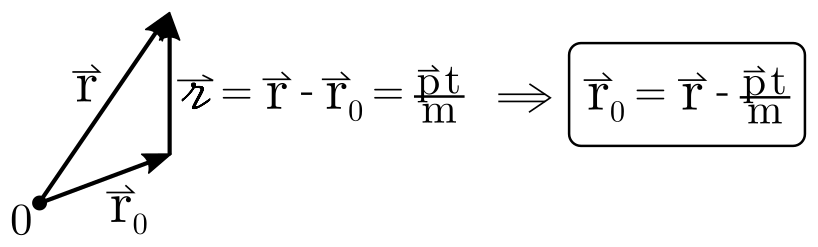
\includegraphics[width=0.7\textwidth]{ballisticExpansion.png}}
	\caption{Ballistic expansion of particles}{Schematic representation particle displacement vectors used to determine how time-of-flight expansion transforms the initial density distibution}
	\label{fig:ballisticExp}
\end{figure}

\hl{make the tof density n'}
the spatial density evolves then \hl{double check $2\pi \hbar$ denom}
\begin{equation}
\begin{split}
n(\vec{r},t) &= \int \frac{d^3\vec{r}\,d^3\vec{p}}{(2\pi\hbar)^3}\frac{1}{\exp{\left[\frac{p^2}{2m} + V(\vec{r}') - \mu\right]\frac{1}{k_BT}}-1}\delta^3\left(\vec{r}-\frac{\vec{p}t}{m}-\vec{r}'\right) \\
&= \int \frac{d^3\vec{p}}{(2\pi\hbar)^3}\frac{1}{\exp{\left[\frac{p^2}{2m} + V\left(\vec{r}-\frac{\vec{p}t}{m}\right)) - \mu\right]\frac{1}{k_BT}}-1} 
\end{split}
\end{equation}

Plugging in the harmonic potential we find that free expansion after release from a harmonic trap is self-similar and amounts to rescaling the the spatial coordinates by \hl{check Demarco's thesis}. Thus the scaled spatial profile is given by
\begin{equation}
n_{th}'(\vec{r},t) = \frac{1}{\lambda_T^3} 
\left(\, \prod_{j=1}^3 \frac{1}{1+\omega_j^2 t^2} \right) 
\Li{\ssfrac{3}{2}}{ \xi \, \exp{\sum_{i=1}^3 \frac{-m\omega_i^2r_i^2}{2k_BT} \frac{1}{1+\omega_i^2t^2}} }
\end{equation}

Using this description of the spatial distribution after time-of-flight expansion, we must now consider how to relate our absorption measurement to the physically relevant variables of the gas.

Finally we must consider the column density along one direction since we are taking absorption images of the atoms. A brief description of absorption imaging and system used for this process is given in \hl{some sec}. 

Simply stated, absorption imaging is the process of illuminating a gas of atoms with resonant (or near resonant) laser light and taking a spatially resolved image of the laser beam. As the light is tuned near a resonant transition, the atoms will absorb and scatter photons out of the original laser beam resulting in a "shadow" which is proportional to the number of scatters within a certain spatial region. This shadow image is then normalized by taking another picture of the laser after the atoms have fallen out of the imaging region. This relation of the light attenuation to the number density of scattering particles is known as Beer's law and results 

Using Beer's law \hl{cite}, we can relate the total absorption of photons to the number density of scattering particles along the optical path multiplied by the absorption cross section. This results in a measurement of the "optical depth" of the gas along a column density. Measurement along a particular direction limits our description of the gas to the two-dimensional plane orthogonal to the laser beam as shown in \hl{some fig from ch 2}.

Experimentally, the optical depth is trivially computed by taking the natural logarithm of the ratio of the images obtained from the camera. We then equate this OD image to be proportional to the spatial density profile after the time-of-flight expansion integrated along the optical path through the atoms.
\begin{equation}
\begin{split}
\text{OD} = \text{ln} \left( \frac{\text{Atom Image}}{\text{Background Image}} \right) &= \sigma_{abs} \int_{-\inf}^{\inf} dz \, n_{th}'(\vec{r},t) \\ 
&= \frac{\sigma_{abs}}{\lambda_T^3} \left( \prod_{j=1}^3 \frac{1}{1+\omega_i^2t^2}\right) \int_{-\inf}^{\inf} dz\,\Li{\ssfrac{3}{2}}{\xi \,\exp{\sum_{i=1}^3 \frac{-r_i^2}{2\sigma_i^2}}}
\end{split}
\end{equation}

where $\sigma_i^2 = \frac{k_BT}{m\omega_i^2}(1+\omega_i^2t^2$. Need to say something about the integral in Eq.\hl{prev} and evaluating the integral along z so going to write out the explicit spatial dependence in cartesian coordinates. Additionally, we'll rewrite the polylogarithm in terms of it's series representation in order to see an identity
\begin{equation}
\int_{-\inf}^{\inf} dz\,\Li{\ssfrac{3}{2}}{\xi \,\exp{\sum_{i=1}^3 \frac{-r_i^2}{2\sigma_i^2}}} = 
\int_{-\inf}^{\inf} dz\, \sum_{n=1}^{\inf} \frac{\xi^n}{n^{3/2}}\exp{\frac{-x^2}{2\sigma_x^2} - \frac{y^2}{2\sigma_y^2} - \frac{z^2}{2\sigma_z^2}}^n
\end{equation}
Defining $\rho=\exp{\frac{-x^2}{2\sigma_x^2} - \frac{y^2}{2\sigma_y^2}}$ and expanding the series out, Eq.\hl{above} becomes
\begin{equation}
=\int_{-\inf}^{\inf} dz\, \xi\rho\exp{\frac{-z^2}{2\sigma_z^2}} + 
 \frac{\xi^2}{2^{3/2}}\rho^2\exp{\frac{-z^2}{2\sigma_z^2}}^2 + 
 \frac{\xi^3}{3^{3/2}}\rho^3\exp{\frac{-z^2}{2\sigma_z^2}}^3 + \cdots
\end{equation}
In this form we can readily separate out the dependence on $z$ and perform the integral making use of the following identity \hl{check identity} $\displaystyle\int_{-\inf}^{\inf} dz\, \sum_{n=1}^{\inf}\exp{\frac{-z^2}{2\sigma_2^2}} = \frac{\sqrt{2\pi}}{n^{1/2}}\sigma_z$. Eq.\hl{above} then reduces to
\begin{equation}
\begin{split}
&=\int_{-\inf}^{\inf} dz\, \sum_{n=1}^{\inf}\frac{\xi^2\rho^n}{n^{3/2}}\exp{\frac{-z^2}{2\sigma_2^2}} \\
&=\sqrt{2\pi}\sigma_z\underbrace{\sum_{n=1}^{\inf}\frac{\xi^n\rho^n}{n^2}}_{\displaystyle\Li{2}{\xi\rho}}
\end{split}
\end{equation}

We are now ready to plug this result for the integral back into the full expression for the optical depth. Retaining the explicit expression in cartesian coordinates, Eq.\hl{above} becomes
\begin{equation}
OD(x,y) = \frac{\sqrt{2\pi}}{\lambda_T^3}\frac{\sigma_{abs} \sigma_z}{(1+\omega_x^2t^2)(1+\omega_y^2t^2)(1+\omega_z^2t^2)} \Li{2}{\xi\,\exp{\frac{-x^2}{2\sigma_x^2} - \frac{y^2}{2\sigma_y^2}}}
\end{equation}
This equation still has one unknown, $\sigma_z$, that we cannot readily measure. This problem is solved by recognizing that we can readily calculate and measure a specific value of Eq.\hl{something}, namely the peak optical depth (OD$_\text{peak}$) located at $x=0,y=0$.
\begin{equation}
OD_{\text{peak}} = \frac{\sqrt{2\pi}}{\lambda_T^3}\frac{\sigma_{abs} \sigma_z}{(1+\omega_x^2t^2)(1+\omega_y^2t^2)(1+\omega_z^2t^2)} \Li{2}{\xi}
\end{equation}
thus the relation between the measured optical depth and the spatial density distribution is given by
\begin{equation}
OD(x,y) = \frac{\text{OD}_{\text{peak}}}{\Li{2}{\xi}}\Li{2}{\xi\,\exp{\frac{-x^2}{2\sigma_x^2} - \frac{y^2}{2\sigma_y^2}}}
\end{equation}
and in the limit of long expansion time during time-of-flight, namely $t \gg \omega_x^{-1}, \omega_y^{-1}, \omega_z^{-1}$ then the measured widths reduce to $\sigma_i^2=\frac{k_BT}{m}t^2$ and the atom temperature is given along each axis by
\begin{equation}
T_i=\frac{m \sigma_i^2}{k_Bt^2}
\end{equation}
Regarding the assumption that the expansion time is much greater then the trap frequencies, we should note that limiting factors in the expansion time are due to center of mass motion of the cloud under the influence of gravity. In the Neutral apparatus we typically utilize drop times are $\approx$ 30 ms. For shallow traps, where $\omega_i$ is be small, then the atoms may not have enough time during expansion to achieve fully ballistic expansion. In these cases it is typical to quote temperatures of the sample as measured along the tightest axis of confinement.

Last thing to do is to relate our expression for optical depth and number density to the total number of atoms in the trap. This task is straightforward by recalling the boson normalization requriement
\begin{equation}
\begin{split}
N&=\int_{-\inf}^{\inf} d^3\vec{r} n_th(\vec{r}) = \int_{-\inf}^{\inf} d^3\vec{r} n_th'(\vec{r},t) \\
&=\int_{-\inf}^{\inf} d^3\vec{r} \frac{\sigma_{abs}}{\lambda_T^3}\frac{1}{(1+\omega_x^2t^2)(1+\omega_y^2t^2)(1+\omega_z^2t^2)} \sum_{n=1}^{\inf} \frac{\xi^n}{n^{3/2}} \exp{\frac{-x^2}{2\sigma_x^2} - \frac{y^2}{2\sigma_y^2} - \frac{z^2}{2\sigma_z^2}}^n
\end{split}
\end{equation}
This equation is the same probem we saw above but integrated over all axes instead of just one. Therefore we can apply the same expansion and identity we employed to solve for the optical depth to find
\begin{equation}
N=\frac{(2\pi)^{3/2}}{\lambda_T^3} \frac{\sigma_x \sigma_y \sigma_z}{(1+\omega_x^2t^2)(1+\omega_y^2t^2)(1+\omega_z^2t^2))}\Li{3}{\xi}
\end{equation}
From our expression for the optical depth, Eq.\hl{some}, we can simply this to
\begin{equation}
N=\frac{2\pi\sigma_x\sigma_y}{\sigma_{abs}}\text{OD}_{\text{peak}}\frac{\Li{3}{\xi}}{\Li{2}{\xi}}
\end{equation}

Eq.\hl{above} 


All of our information comes from taking pictures of our atomic clouds and inferring the physical properties of the gas before the time-of-flight expansion. This is possible since we know the density profile of the gas in-situ. In the absence of external fields, other than gravity, turning off the trapping potential results in ballistic expansion described by $\vec{r} = \vec{r}_0 + \frac{p^2}{2m}t$, where $\vec{r}_0$ and $p$ are the position and momentum at the moment of release from the trap and $t$ is the expansion time. Neglecting the center-of-mass motion due to gravity and assuming long expansion times, then we can easily find a regime where $\frac{p^2}{2m}t \gg \vec{r}_0$ and therefore
	\begin{equation}
		\vec{r} \approx \frac{p^2}{2m}t
	\end{equation}
This 

 \cite{Ketterle1999} \hl{get demarco thesis?}. Thus, for atoms 

Thus, for atoms starting at a position $\vec{r_0}$ 

Density profile expands self-similarly 

Time of flight is essentially a Fourier transform which turns the initial momentum information into spatial information.



\section{Characterizing collisions} \label{sec:cold_collisions}
understand how to treat quantum two-body problem with external field coupling

Collisions are one of the key ways we learn things about atoms 

In atomic physics, our low density gases are mainly within the regime of small interactions. 

Here is where I cite sources of some of the original PA work, feshbach stuff

collisions as an interferometer of the incoming and outgoing off the barrier, but also of different partial waves.

I want the reader to know that PA dis concerning the scattering wavefunction, that it comes from the overlap integral of the tweo wavefunctions (why do I need to know this? nbecause this means that it is sensitive to positions of the nodes and can be used to map out the potentials. \hl{this will motivate discussing low energy physics}

This spatial dependence is mapped onto the internal energy levels of each atom. I want to say dressed state model here (review atom-photon coupling, atomic physics book).


\subsection{Classical} \label{ssec:classical}
cross sections
			as a measure of the time between collisions
			
		potentials
			where they come from
		centrifugal barrier
			analog - slide 16 Julienne
			just rxp of particles
			
		center of mass coordinates
			only care  about relative (generally)
			simplifies calculations

\subsection{Single channel scattering} \label{ssec:single_chan}
quantum
	solve time0independent SE
	just need potential, basis set, and boundary conditions
		
structureless pasrticles scattering
	free space
		plane waves
		de Broglie wavelength
			strontium de Broglie at 1uK
	
	delta function
		unitarity limit
		supports one bound state - the true halo state
		where the wavefunction comes from

	r-dependent potential
		show 1.1 from Hutson
		gneerally very complicated between atoms
			long-range part is typically has a power law drop off
			important that V->0 as R-> inf
		for ground state atoms dominant long-range part is R6
		
	scattering states (E>0)
		replusive barrier - particle scatter
		attrative well - particles accelerate
		
	bound states
		boundary conditions dictate
		might have quasibound states (shape resonances)
		
	wavefunctions
		General appraoch is incoming plane wave plus spherical wave
			
		common appraoch to expansion of wavefunction in partial wave expansion
			redefine SE in terms of partial waves
				Asymtotic solution from WKB
					V->0 so must go to plane wave
					See phase shift
					
		total cross section as sum over all partial waves

%%%%%%%%%%%%%
this results in a poitential that supports bound states. 

consider the two particle system as a single entagled particle
	long range part of this quasi-particle is just the eigenstates of the separate particles themselves (only composed of two parts)
	but the short range part is going to be determined by some complex physics (new eigenstates, what is the coupling mechanism?)
		the vdW point is the boundary distance?
		coupling is due to the interatomic potential, there is at least the long-range part falling off as R6, what are the types of interactions which make up the internal wall?

\subsubsection{Low energy results} \label{sssec:sold_single_chan}

Simple form for scattering length
	gives limits on cross sections
	slide 24 (not sure I get the upper bound bit)

scattering length is a phase accumulation
	scattering length is very sensitive to details of potential
		can't really calculate ab initio
		
	a number that represent all the complex physics within the interaction region
	
	simple interpretation as peak shift at long range
		slide 12 julienne
	
Another way of seeing the origin of a is as the collisional E goes to zero
	wavefunction should go to a straight line
		plot from bertlett
	a is the intercept of that line on the internuclear axis
		this is one of the methods of actually determining a

the scattering length as a coupling parameter in length units
	The mean field energy (I think I had a reference on this)
	slide 26

Determmining a is not so easy because the interatomic potential is not known
	this was one of the pioneering use for photoassociation
	PA is sensitive to the collisional wavefunction and therefore can help to map out the spatial distribution of the ground state
Simple WKB estimation predicts zero-energy bound state as E->0
	every atom would have infinite scattering length at low energy
	obviously not the case, GF first to determine analytic corrections due to long-range vdW interaction
		comes about because of phase contribution from the long-range part
This is the regime we explored with our work in chapter 4
	probing a bound state just near the dissociation threshold makes us extremely sensitive to the entire phase of the well


free atoms
scatering as single particle state (differnet eigenstate)
	interaction determined by some gnarly stuff
From scattering theory we know that the long range behavior is determined by short range physics
	how do we know this? (the dalibard intro)
Can we come up with good enough pseudo potentials to describe the short range physics and then solve the schrodinger equation to extract wavefunctions?
	we want wavefunctions because that is the full characterization
	we don't know the right eigenbasis for the short range part but we can make some guesses (in particular Hund cases setup eigen states for various possible internal states)
	Bohn and Julienne theory guessed based on using quantum defect theory
		this pre-supposes that the bound and free wavefunctions are similar (I forget in what respect) but that the bound ones must go to zero as R->Inf
If we have some notion of the wf then we can construct matricies which define interactions once we add additional coupling to the scattering problem


now in a position where I need to connect scattering theory and the PAS


Once we have the ground state wavefunction of our new particle we can construct the internal structure by considering the internal energy strucutrue of the constituent atoms
	Can I make a connnection that since it is a composite particle we must consider all the various configurations available?
	
\begin{figure} \label{fig:ch3_sr_scat_wf}
	\centerline{
	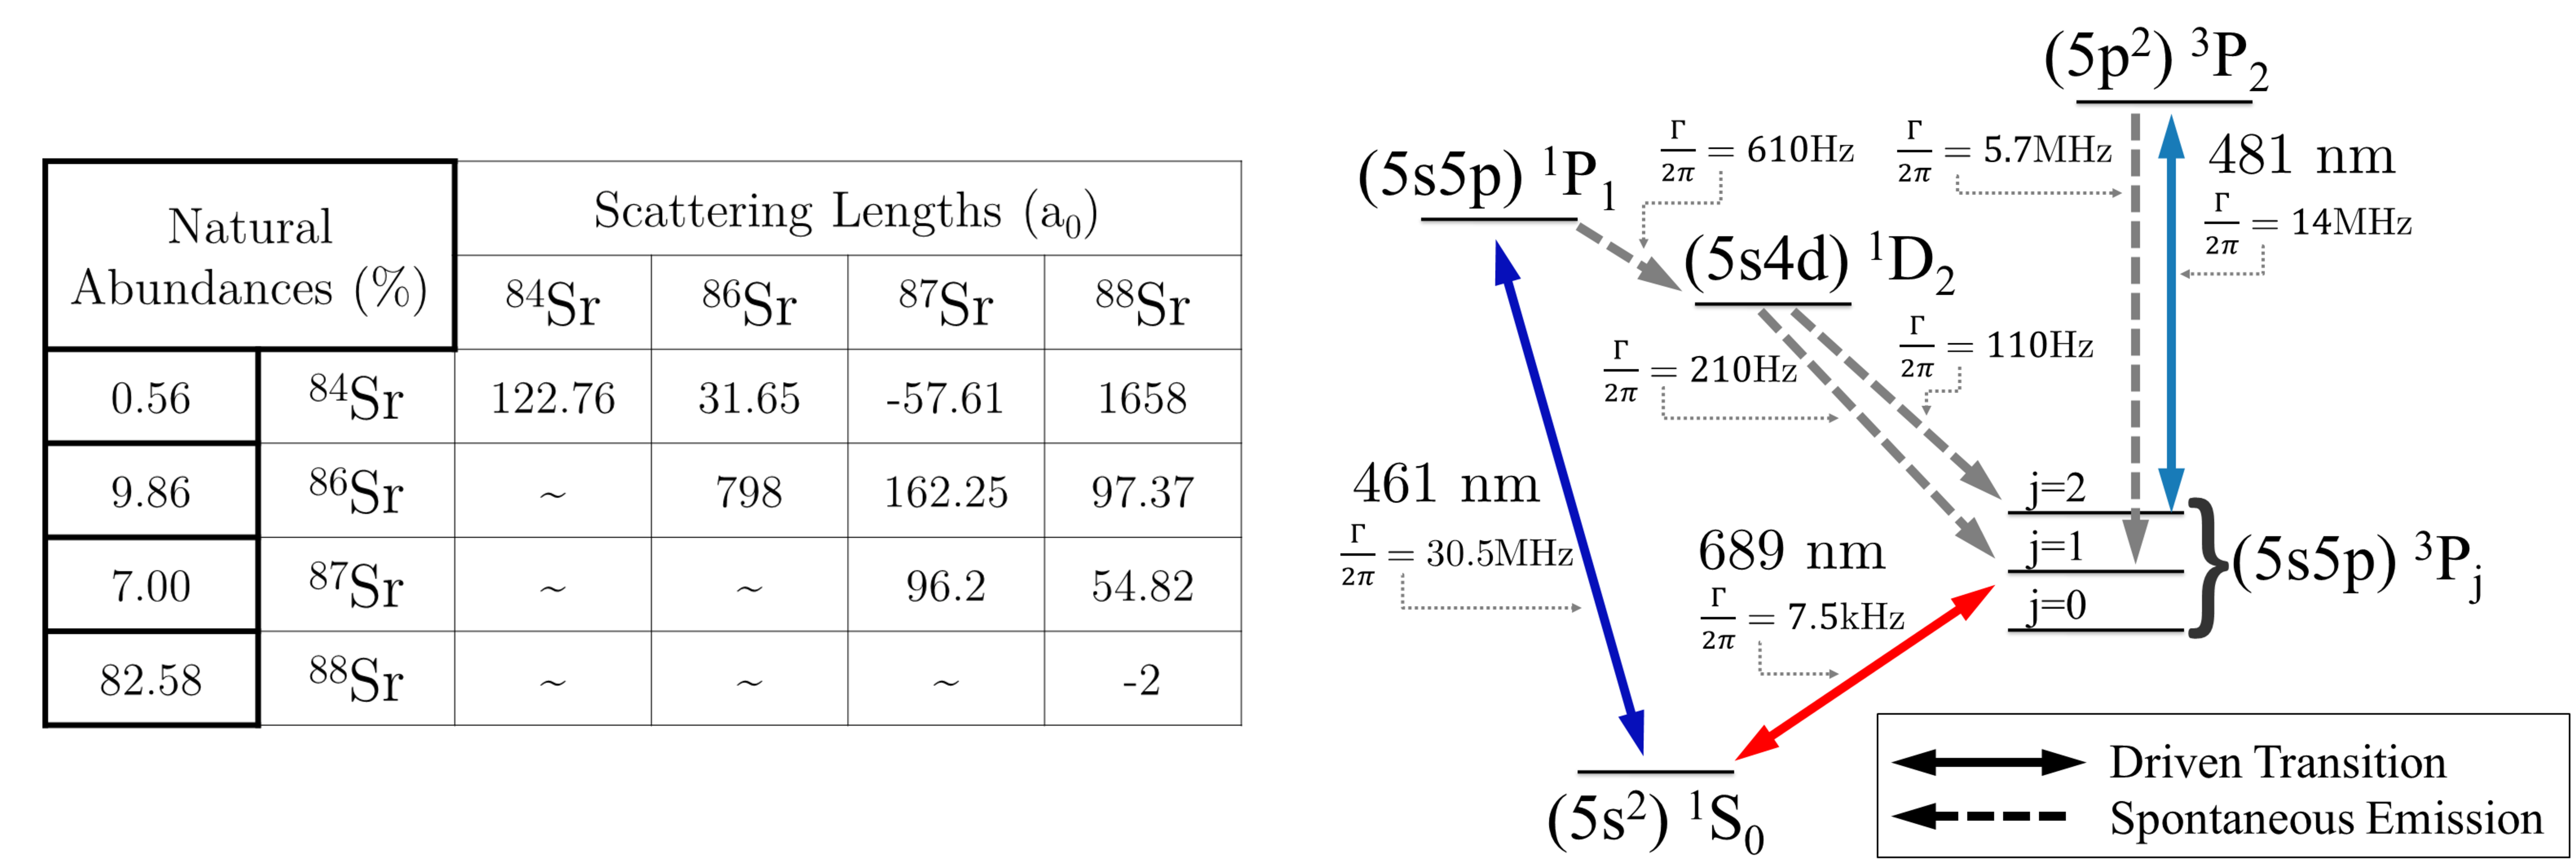
\includegraphics[height=0.25\textheight]{strontium_properties.pdf}}
	\caption{Strontium interatomic wavefunctions}{Res 6.3}
\end{figure} 

\subsection{Multichannel scattering} \label{ssec:multi_chan}
Everything we discussed was for unstructured particles
	this is the power of the scattering length
	
this would be the end of the story if all of these potentials were "separable" (or independent)
	you'd find your configuration, describe the potential, solve it, and you're done
of course this isn't actually the case because the eigenstates of the separate potentials couple to one another.
Even understanding the natural coupling between coupling between potentials is not easy
	tie back to complexity of understanding short range physics
		We don't really know what coupling exist and which energy levels are most important
	mostly effects the bound states of the system
	strontium example of the D state coupling in the 3P1 potential
		references to Res and other work

address somewhere that these types of problems are generally solved via coupled-channel methods which follow the same recipe for the scattering problem as in the single channel case but does so considering all channels simultaneously through matricies defining potentials and their couplings to one another.
coupled equations are complicated
	point out references from Julienne, Mies, Bao, Hutson
	
But can match at aymptotic wavefunction again and get a lot of insight
	
example: multichannel use to describe atom-diatom coupling
	mutli-channel model (normal MFR diagram)
		other potentials are due to different combinations of atoms in hyperfine states
	these potentials can have different magnetic moments
		means that addition of a magnetic field can tune them relative to one another
MFR has been extensively studied and is a common tool used in atomic physics
	
scattering resonances are due to off diagonal coupling between bound closed channels and scattering open channels
	give picture
hand wavy expalanation is that bringing a bound state close will modify the open channel (potential?)
	this results in a tweak of the phase shift which results in a change in scattering length
can describe this as a change in the elastic cross section of the incoming open channel
in general there is also an inelastic cross section that may contribute if the bound state has a finite lifetime.
	
define open and close channels		

S matrix - defines scattering phases and ampltiudes due to couplings between various open and closed channels
	S found from the asymptotic solutions

if single channel then S reprodcues above results
if inelastic then get complex scattering length (need better way to segue, Julienne 2014 slide 19 - unitarity argument maybe)
complex scat
	Real part is the elastic cross section
	Imag part if the inelastic



Also the Chin '10 review on feshbach resonances

Follow the Nicholson 15 paper method of introing the elastic and inelastic cross sections

The use of a laser field as the coupling scheme in a Feshbach resonance introduces several advantages and complexities that must be considered when determining the expected properties of optical Feshbach molecules. In order to understand these differences, we will briefly outline the key concepts behind Feshbach resonances and the distinctions between optical and magnetic Feshbach resonances.


\begin{figure} \label{fig:FeshbachCartoon}
	\centerline{
	\includegraphics[width=\textwidth]{feshbachCartoon.pdf}}
	\caption{Schematic representation of a Feshbach resonance}{(a) Potentials for the open ($^1S_0\!+\!^1S_0$) and closed ($^3P_1\!+\!^1S_0$) channel of an optically coupled Feshbach resonance in strontium. (b) The same coupling shown in (a) in the dressed state model. Tuning of the excited potential is achieved by varying the laser frequency detuning, $\delta = \omega_p - \omega_{bound}$, and $\omega_{free}$ is the $^1S_0\!\rightarrow\!^3P_1$ atomic transition frequency.}
\end{figure} 
	

The basic idea of a Feshbach resonance is outlined in Fig.\;\ref{fig:FeshbachCartoon}. Consider a simple two channel system, denoted by the open channel and the closed channel. The open channel is generally a ground state potential for two free atoms near threshold. Atoms occupying this state can undergo elastic collisions and, in the absence of any external perturbation, will remain in the open channel. Conversely, the closed channel is a bound state of a higher lying potential who's energy can be tuned relative to the open channel. In the absence of coupling between the states, the open and closed channel remain eigenstates of the system as the tuning parameter, and therefore the energy of the closed channel, is changed. However, in the presence of coupling between the channels, the original eigenstates are mixed and develop an avoided crossing between the bare open and closed channels, when tuned across the resonance. The power of Feshbach resonances comes from the ability to externally manipulate the degree of state mixing, which results in control of the s-wave scattering length and the creation of low energy Feshbach molecules.

Magnetic Feshbach resonances (MFR) are used extensively in alkali metal systems to tune the scattering properties of ultracold gases since the ground states of these systems feature a magnetic moment due to an unpaired electron in the valence shell. Thus, MFRs utilize interactions between low lying ground state molecular potentials via spin-dependent couplings. Since both the open and closed channel are ground state potentials, MFRs often exhibit extraordinarily long lifetimes \cite{Chin2010,Kohler2006}. Conversely, in strontium the ground state is a $^1S_0$ state, as shown in Fig.\;\ref{fig:energy_level_diagram}. This state is not magnetically sensitive, so no MFRs exist near the $^1S_0\!+\!^1S_0$ interatomic potential. Fortunately, optical Feshbach resonances (OFR) serve as another method to introduce coupling between the ground state potential (open channel) and a molecular state of an electronically excited potential (closed channel). Our work has utilized coupling between the $^1S_0\!+\!^1S_0$ and  $^3P_1\!+\!^1S_0$ two-body potentials via the narrow $^1S_0\!\rightarrow\!^3P_1$ atomic transition at 689nm. Fig.\;\ref{fig:FeshbachCartoon} shows a schematic of the potentials involved in the OFR of strontium in both the bare atomic and dressed state pictures. In the dressed basis we consider the combined atom + photon field system such that the channels become $\ket{^1S_0\!+\!^1S_0\!+\!n_p\hbar\omega_p}$ as the open channel and $\ket{^3P_1\!+\!^1S_0\!+\!(n_p-1)\hbar\omega_p}$ for the closed channel. As the light field frequency, $\omega_p$, is varied the excited closed channel potential will experience an energy shift relative to the open channel, resulting in resonant coupling between the open and closed channels. \cite{Ciuryo2005,Bohn1997,Fedichev1996a}

Both MFRs and OFRs can be treated by the same theoretical formalism, as a modification of the collisional properties between two particles \cite{Nicholson2015a,Chin2010}. One of the hallmarks of ultracold physics is the simplicity of atomic collisions. As bosonic atoms get colder they can only collide via $\ell=0$ partial waves and thus the elastic collision rate between two atoms becomes energy independent and can be parameterized by a single fixed quantity, $a_s$. This parameter is known as the s-wave scattering length and is determined by the short range molecular potential between two colliding atoms. Through a similar approach, collisions near Feshbach resonances can be modeled by introducing a complex s-wave scattering length, $\tilde{\alpha}$. In this model, the magnitude of $\tilde{\alpha}$ influences the elastic scattering rate between particles while the imaginary part describes losses through inelastic scattering. Under an isolated Feshbach resonance model at low energies, this complex scattering length is given by \cite{Chin2010}
	\begin{equation} \label{eq:complexScatter_constant}
		\tilde{\alpha} = a - ib = \frac{a_s \Gamma_0}{-E_0 + \imath (\gamma/2)}
	\end{equation}
where $E_0$ and $\Gamma_0$ are the energy independent parameters for, respectively, the resonance position and coupling strength between channels, and $\gamma$ is a general decay term associated with loss from the closed channel. Using Eq.\;\ref{eq:complexScatter_constant}, we can note the two main differences between MFRs and OFRs. Most experimentally useful MFRs, such as in Li and K, have negligible closed channel decay, $\gamma = 0$, and a fixed coupling strength between the open and closed channels. Thus, the change in the s-wave scattering length takes on a particularly simple form, 
	\begin{equation} \label{eq:MFRscatter}
		\tilde{\alpha} = a_s \left( 1- \frac{\Delta}{B - B_0} \right)
	\end{equation}
where $B_0$ is the resonance position and the coupling strength is parameterized by a magnetic width $\Delta$, such that $\Gamma_0 = \delta \mu \Delta$ with $\delta \mu$ the difference in magnetic moments between the open and closed channel. 

Conversely, OFRs offer the possibility to tune the coupling strength between the open and closed channel, since the coupling depends on the transition matrix element which varies with the square root of laser intensity. Furthermore, since OFRs utilize electronically excited states which have a natural lifetime, $\gamma$ is nonzero. This results in inelastic loss processes for OFRs. Similar to MFRs, we can define the change in scattering length as \cite{Nicholson2015a,Yan2013c,Blatt}
	\begin{equation} \label{eq:OFRscatter}
		\tilde{\alpha} = a_s \left( 1 - \frac{w \delta}{\delta^2 + \gamma^2/4} + \frac{i}{2} \frac{w \gamma}{\delta^2 + \gamma^2/4} \right)
	\end{equation}
where $\delta=\omega - \omega_0$ is the detuning from the chosen photoassociation resonance at $\omega_0$ as shown in Fig.\;\ref{fig:FeshbachCartoon}, and the width of the resonance is defined by $w = -\ell_{opt} \, \gamma / a_s$. Typically, the strength of OFRs are characterized by their optical length \cite{Nicholson2015a,Chin2010} given by $\ell_{opt} = a_s \Gamma_0 / \gamma = \frac{\lambda_{OFR}^3}{16 \pi c} \frac{ \left| \left< n | E \right> \right|^2}{k} I$. Here $c$ is the speed of light, $\lambda_{OFR}$ is the wavelength of the coupling laser, and $\left| \left< n | E \right> \right|^2$ is the free-bound Frank-Condon factor between the bound state $\bra{n}$ and scattering state $\ket{E}$. Additionally, it is useful to identify the real and imaginary parts of Eq.\;\ref{eq:OFRscatter} as defined in Eq.\;\ref{eq:complexScatter_constant}.
	\begin{equation} \label{eq:OFRparts}
		 a_{\scriptscriptstyle OFR} = a_s + \ell_{opt} \gamma \frac{\delta}{\delta^2+\gamma^2/4} \qquad
		 b_{\scriptscriptstyle OFR} = \frac{\ell_{opt}}{2} \frac{\gamma^2}{\delta^2+\gamma^2/4}
	\end{equation}

Our previous work exploring the use of an optical Feshbach resonance took advantage of photoassociation transitions with large optical lengths to control the scattering length of an $^{88}$Sr BEC as described by Eq.\;\ref{eq:OFRscatter}. However, all studies of OFR to date have been limited by large atom loss rates \cite{Thalhammer2005,Theis2004,Fatemi2000,Blatt,Yan2013c} which can be modeled as a density evolution, $\dot{n} = -K_{in}n^2$, where $K_{in}$ is the two-body inelastic loss rate constant. In the low energy limit, $k\!\rightarrow\!0$, the inelastic loss rate is given by
	\begin{equation} \label{eq:K_in}
		K_{in} = \frac{8 \pi \hbar}{\mu_{r}} b_{\scriptscriptstyle OFR} = \frac{4 \pi \hbar}{\mu_r} \frac{\ell_{opt} \gamma^2}{\delta^2 + \gamma^2 / 4}
	\end{equation}
where $\mu_r$ is the reduced mass, $\delta$ is the laser detuning as shown in Fig.\;\ref{fig:FeshbachCartoon}.


\section{Modeling of photoassociation lineshapes} \label{sec:bohn_and_julienne}

This section will concern the general theory used to describe photoassociative spectra. While a full quantum close-coupling calculation is the most complete and rigorous method for analyzing cold quantum scattering problems, useful approximations can be applied to realize relatively more "simple" closed analytic formulas describing photoassociation spectra. 

This section will cover the theory of lineshapes in PAS.

Somewhere I read about three regimes of PAS as a comparison of relevant energy scales. Should explore that here

Pretty much have everything needed from our previous section.
Relation of rate constant to cross sections is nice and simple
		Julienne 14 - slide 21
These fully coupled-channel models are not straightforward to evaluate.
	Can make assumption to simplify




\subsection{One-photon excitation of free to bound transitions} \label{ssec:one_color_pa}

Can recreate the type of model for MFR in a field dressed approach
	plot showing photon + potential
	

	
ANalytic forms for modeling
	compare all the forms of K
		the crazy one from BJ 99
		the simple one with f(p)
		nicholson 42
	

show plot with all the terms defined

give loss rate (will need to have introduced before)
	define terms
		gammaStim as overlap
		gamma as molecular lifetime
		delta as detuning
		A as coupling strength
	
introduce reflection approximation
	evaluation of overlap
	reference BJ 99
	
give relative momentum distribution
	this results in an asymmetric profile
	give plot
	
Number equation vs. time

segue to narrow lines


\subsubsection{PAS near narrow intercombination transitions} \label{sssec:narrow_pa}

quick note on the usage of the relative momentum distribution
			usually this is all we care about since the CoM part results in doppler shifts which would be neglible on the energy scales of broad dipole-allowed transtions
			using narrow intercombinations lines, the photon recoil energy is comparable to the bound state lifetime
				this means that indivual lorentzians might be shifted (each by a different amount) in addition to the total line shape being asymmetric
			Integration over both degrees of freedom will be an important discussion in the next chapter as we fit spectra and determine the halo binding energy

ideas of limiting cases that can be explored with PAS \cite{Ciuryo2004}

\subsection{Extension to two-color spectra} \label{ssec:two_color_pa}

Pretty much the same things
		
Show new picture with all the couplings defined


Now that we have the theory of PAS covered. 



\begin{equation}\label{eq:number}
   N(t)={N_0 \rm{e}^{-\Gamma t} \over 1+
   {2 N_0 \langle K \rangle V_2\over \Gamma V_1^2}(1-\rm{e}^{-\Gamma t})}
\end{equation}
where  $N_0$  is the number  at the beginning of the PAS interaction
time, and $\langle K \rangle$ indicates a spatial average of collision event rate constant $K$ (Eq.\ \ref{equationKeffective}). The one-body loss rate, $\Gamma$, is due to background
collisions and off-resonant scattering from the PA lasers.

PA loss is described with a local equation for the evolution of the atomic density [Eq.~(\ref{densitydecay})]. Integrating Eq.~(\ref{densitydecay}) over the trap volume yields the time evolution of the number of trapped atoms [Eq.~(\ref{number})]. The effective volumes used throughout this analysis are defined by
\begin{equation}\label{eq:effectivevolumes}
	V_{\text{q}}=\int_{\mathrm{V}} d^3r \, e^{-\frac{qU(\mathbf{r})}{k_{B}T}},
\end{equation}
for trapping potential $U(\mathbf{r})$. The collision event rate constant can be expressed as a thermal average of the scattering probability for loss, $\vert S(\epsilon,\omega_1,\omega_2,...,\mathbf{r})\vert^2$, over the collision energy $\epsilon$. We also average over the trap volume to allow for the possibility that the scattering probability can vary with position in the trap due to inhomogeneity of laser intensity profiles and the density distribution [Eq.~(\ref{equationKeffective})].

%This yields
\begin{eqnarray} \label{equationKeffective}
% \nonumber to remove numbering (before each equation)
  \langle K \rangle&=& \frac{1}{V_{2}}\int_{\mathrm{V}}
d^3r \,
          e^{-\frac{2U(\vec{r})}{k_{B}T}} \nonumber \\
         &&\times \frac{1}{h\,Q_{T}}
\int_{0}^{U_{max}-U(r)}d\epsilon \vert S\vert^2
   \,e^{-\epsilon/k_{B}T}.
\end{eqnarray}
%\begin{equation}\label{Kintegral}
%   K=\frac{1}{h\,Q_{T}} \int \vert S(\epsilon,\omega_1,\omega_2,...)\vert^2
%   \,e^{-\epsilon/k_{B}T} \; d\epsilon,
%\end{equation}
where the partition function is $Q_{T}=\left({2\pi k_{B}T \mu \over
h^2}\right) ^{3/2}$ for reduced mass $\mu$.


Bohn and Julienne \cite{bju96} provide an expression for $\vert S(\epsilon,\omega_1,\omega_2,...)\vert^2$ for a collision on the open channel of two ground state atoms (g) with total energy $\epsilon$ leading to loss-producing decay from the excited state $b_1$ with rate $\gamma_1$. (See Fig.\ \ref{PASDiagram}.) It yields
\begin{eqnarray}\label{equationSprob}
  \vert S\vert^2 =   \hspace{2.5in}&&\\
  {(\Delta_2+\epsilon/\hbar)^2{\gamma}_1{\gamma}_s \over
  	\left[(\Delta_1+\epsilon/\hbar)(\Delta_2+\epsilon/\hbar)-\frac{\Omega_{12}^{2}}{4}\right]^2+\left[ \frac{\gamma_1+\gamma_s}{2}\right]^2(\Delta_2+		 	\epsilon/\hbar)^2}, &&\nonumber
\end{eqnarray}
where all quantities are defined in the main text. For simplicity, we have omitted the light shift of $b_1$ due to coupling to the scattering continuum \cite{bju99}. Equation (\ref{equationSprob}) neglects all light shifts due to the trapping laser. Light shifts due to the photoassociation lasers coupling to states outside our model (Fig.\ \ref{PASDiagram}) are also neglected. The thermal energy is much greater than the zero-point energy for trap motion, $T\gg h\nu_{\text{trap}}/k_B$, so confinement effects are negligible \cite{zbl06}.

%$\Delta_1=\omega_1-E_{b1}/\hbar$ and $\Delta_2=\omega_1-\omega_2-E_{b2}/\hbar$ are the one-photon detuning from state $b_1$ and two-photon detuning from state $b_2$ respectively for initial scattering state with $\epsilon=0$.

%, which is a good approximation for our experiment because the light shift of state 1 is small compared to the detuning $\hbar \Delta_1$,
and lights shifts of states 0 and 2 are approximately equal and will cancel in the determination of the binding energy of the halo state, $E_2$ \cite{rbm04,rfk87}. Neglecting

%We record spectra by varying $\Delta_2$ at fixed detuning from the intermediate state $\Delta_1$

For the experiments reported here, we maintain significant intermediate-state detuning, $|\Delta_1|\gg |\Omega_{12}|$. Thus we are in a Raman configuration, and near two-photon resonance the expression for the scattering probability for a given initial scattering energy Eq.~(\ref{equationSprob}) can be approximated as a Lorentzian
\begin{eqnarray}\label{equationSprobLorentzian}
 \vert S\vert^2 \approx {A(\epsilon) \over
 \left(\Delta_2+\epsilon/\hbar-\frac{\Omega_{12}^{2}}{4(\Delta_1+\epsilon/\hbar)}\right)^2+\left[ {\Gamma_L(\epsilon)}/{2}\right]^2},
\end{eqnarray}
where $A$ and $\Gamma_L$ are defined in Eqs.\ (\ref{ApproxLorentzianQuantitiesMain}) and (\ref{ApproxLorentzianQuantities-2Main}).

As discussed in the text, we analyze loss spectra using the effective expression, Eq.\ (\ref{equationApproxLorentzian}) to account for possible deviations from the single-channel theory \cite{bju96}.

%\section{AC Stark shift due to excitation lasers}
\label{App:ACStark}
The total 689-nm intensity oscillates with 100\% contrast according to
$I_{total}=I_1+I_2+2\sqrt{I_1I_2}\cos \left[(\omega_1-\omega_2)t \right]=2I\left\{1+\cos \left[(\omega_1-\omega_2)t \right]\right\}$.
Equation \ref{Eq:ACStarkFullModel}
The form of the AC Stark shift
due to excitation lasers in Eq.\ \ref{Eq:GlobalFit}
 reflects the time average of the intensity and neglects the interference term. To confirm that this is the correct description, we numerically solved the time-evolution for a three-level system with similar optical couplings and oscillating optical intensity as present during halo photoassociation. The Hamiltonian is
\begin{eqnarray}\label{Eq:ThreeLevelHamiltonian}
H= \hspace{3in} \\
 \nonumber\\
\left(
    \begin{array}{ccc}
      0 & \Omega_{01}\left[\mathrm{cos}(\omega_1 t)+ \mathrm{cos}(\omega_2 t)\right] & 0 \\
      . & E_{b1} & \Omega_{12}\left[\mathrm{cos}(\omega_1 t)+ \mathrm{cos}(\omega_2 t)\right] \\
      . & . & E_{b2} \\
    \end{array}
  \right)
\nonumber
\end{eqnarray}
For  $\Omega_{01}\ll \Omega_{12} \ll \Delta_{1}\equiv E_{b1}/\hbar-\omega_1$, which is analogous to the  experimental conditions used here

, the shift of the two-photon resonance condition follows $\delta={\Omega_{12}^{2}}/{2\Delta_{1}}$ in agreement with Eq. \ref{Eq:ACStarkFullModel}.


%% ARCHIVE
%%%%%%%%%%%%%%%%%%%%%%%%%%%%%%%%%%%%%%%%%%%%%%%%%%%%%
%Think I want to introduce the photoassocation by talking about the collisional wavefunction

%what will that do?

%I want to build up ideas about the FCF and need the wf for that
%	to get qf I have to go back to scattering theory

%ideas of the wavefunction become that basis for how you want to talk about interacting potentials
\chapter{High-intensity photoassociation spectroscopy of a halo molecule} \label{ch:chap4}
\section{Probing the ground state potential} \label{sec:highE_intro}
In this chapter we study the least-bound vibrational level of the X$^1\Sigma_g^+$ electronic ground state of the $^{86}$Sr$_2$ dimer in a high-intensity regime.
Previous studies of the molecular states of the X$^1\Sigma_g^+$ ground state potential have been performed using strontium-88, due to its high natural abundance, and strontium-84, because of it's amenable scattering properties. \cite{Reinaudi2012, McGuyer2014, McGuyer2015a, rom12, Stellmer2012}.

This work presents the first two-photon photoassociation study of the ground state of $^{86}$Sr.
All previous PA experiments with this isotope have been one-photon photoassociation to excited electronic states \cite{Mickelson2005,Borkowski2014a,Reschovsky2018}.
The large $s$-wave scattering length, $\sim$800\,a$_0$, for this isotope is indicative of a near-threshold bound state known as a halo molecule.
Direct photoassociation to this halo state revealed several unanticipated phenomena discussed in this chapter including AC Stark shifts comparable to the halo molecule binding energy and multi-photon resonance processes \cite{Kon2018}.

This work is expanded upon in Ch.\,\ref{ch:chap5} with a low-intensity study that precisely determined the halo binding energy and using this measurement, improves upon the previous best determinations of the scattering lengths of all strontium isotopes via mass-scaling.
In these initial experiments, we explore some of the novel effects of photoassociation to a halo state with a focus on understanding the AC Stark shifts and developing a useful theoretical framework for describing this unique photoassociation regime.

As discussed in previous chapters, two-photon PAS can be used to directly populate molecular levels and may be described with the formalism of Bohn and Julienne \cite{Bohn1999}.
However, this approach assumes the two driving lasers are of sufficiently different frequencies that each independently drives a specific transition, as in the typical $\Lambda$-model \cite{Wynar2000, Bohn1996}.
In the regime of PAS to a halo state, the laser frequencies differ by only up to $\sim\!300$\,kHz, much smaller than the typical intermediate state detuning of several MHz.
Thus, both lasers must be considered to act on each leg of the transition simultaneously.
The effects of this two-frequency coupling were explored through a collaboration with the theory group of Kaden Hazzard to develop simple models that are able to reproduce the key experimental observations and features.

In the following, we present the experimental results of high-intensity PAS to the halo state and develop lineshape models based on the theory of Bohn and Julienne to extract the halo state binding energy.
Next, we'll compare our experimental data to numerical simulations of a three-level model.
This model subsequently becomes the basis of a Floquet treatment which results in an analytic form for describing and predicting AC Stark shifts of the halo state.
This is used to consider the observed frequency dependence of the halo state energy and estimate the bound-bound coupling strength between the intermediate and halo states.

\section{Experimental setup} \label{sec:highE_methods}
	\begin{figure} 
	\centerline{
	  \includegraphics[width=\textwidth]{sr_pa_potential.pdf}}
	  \caption{$^{86}$Sr$_2$ halo molecule excitation scheme}{Two-photon photoassociation diagram. The energy of two well-separated $^1S_0$ atoms at rest is taken as zero. $\epsilon$ is the kinetic energy of the colliding atom pair. $E_{b1}$ is the unperturbed energy of the bound state of the excited molecular potential that is near resonance with the free-bound laser, which in these experiments is the second-least-bound level of the excited molecular potential $\nu=-2$. $E_{b2}$ ($<0$) is the energy of the least-bound state of the ground molecular potential. The photon of energy $\hbar \omega_1$ is detuned from $E_{b1}$ by $\hbar \Delta_1$ for $\epsilon=0$, while the two-photon detuning from $E_{b2}$ is $\hbar \Delta_2$. The decay rate of $b_1$ is $\gamma_1$. Stark and collisional frequency shifts are neglected in this schematic.}
	  \label{fig:PASDiagram}
	\end{figure}
Fig.\,\ref{fig:PASDiagram} shows the excitation scheme used to probe the halo state in $^{86}$Sr using two-photon Raman photoassociation \cite{Jones2006}, in which two laser fields couple colliding atoms to the least-bound state of the ground molecular potential. 
%The sample temperature is low enough that collisions are entirely $s$-wave. 
$^{86}$Sr has no nuclear spin and a $^1S_0$ electronic ground state, leading to a single X$^1\Sigma_g^+$ ground electronic molecular potential.
The target state for the two-photon transition has total angular momentum $J=0$ and halo state energy $E_{b2}(<0)$, which we label as $b_2$.
The dominant intermediate state, $b_1$, with energy E$_{b1}$, is the $J=1$ rotational state of the second least-bound $\nu=-2$ vibrational level on the $0^+_u$ molecular potential, which asymptotically connects to the $^1S_0\,+\,^3P_1$ asymptote at long range \cite{MartinezDeEscobar2008}.
This state is bound by $44.246(10)$\,MHz \cite{Borkowski2014a, Reschovsky2018}.
We define $\Delta_1=\omega_1-\text{E}_{b1}/\hbar$ and $\Delta_2=\omega_1-\omega_2-\text{E}_{b2}/\hbar$ as the one-photon detuning from state $b_1$ and two-photon detuning from state $b_2$ respectively for an initial scattering state with collision energy $\epsilon=0$.
The Rabi frequency, $\Omega_{2,12}$, characterizes coupling between states $b_1$ and $b_2$ due to the laser field at $\omega_2$ with single-beam intensity $I_2$.
Because the binding energy of the halo molecule is very small compared to $\Delta_1$, both laser frequencies are near resonance with the $\nu=-2$ state. 
The least-bound $\nu=-1$, $J=1$ excited molecular state, bound by $1.633(1)$\,MHz, and the excited atomic state lie near enough in energy to the $\nu = -2$ state that they can also effect our observations.	

The small detuning between $\omega_1$ and $\omega_2$ results in an atypical consideration of the accessible resonance conditions during the Raman process.
Fig.\,\ref{fig:haloResProcess}a shows the two scenarios which lead to resonance with the halo state when $\omega_1$ is held fixed and $\omega_2$ is varied.
	\begin{figure}
	\hspace*{-0.05\textwidth}  
	\centerline{
	  \includegraphics[width=1.1\textwidth]{excitationScheme.pdf}}
	  \caption{Accessible halo resonance PAS processes}{Effects of fixing $\omega_1$ and varying $\omega_2$. Consider the state \ket{b2} to be fixed. a) The left and right panels illustrate scanning $\omega_2$ relative to $\omega_1$. Within each panel, the lasers start with $\omega_1 = \omega_2$ and $\Delta_2 = -E_b/\hbar$. Scanning $\omega_2$ will fulfill the resonance condition in both scenarios but also lead to a change in $\Delta_1$ if $\omega_1 > \omega_2$.  b) Example simulated spectra compared with experimental PAS. The development of the model is described in Sec.\,\ref{sec:highE_theory}. For both simulations, the "positive" axis is the configuration where $\omega_2 \geq \omega_1$ and the negative axis is the opposite. Note the asymmetry in the resonance frequency for $I=0.66$\,W/cm$^2$.}
	  \label{fig:haloResProcess}
	\end{figure}
The left panel, when $\omega_2 \geq \omega_1$, shows $\Delta_1$ remains fixed while scanning the two-photon energy.
This holds constant the bound-bound coupling between the halo and intermediate state.
In the opposite case, when $\omega_2 \leq \omega_1$, the halo resonance condition can still be satisfied as $\omega_2$ is varied, though at the expense of also varying $\Delta_1$.
This behavior is equivalent to fixing $\omega_2$ and scanning $\omega_1$ in a typical $\Lambda$-type Raman scheme, but warrants our attention because of the interchangeability of the excitation lasers.

The latter configuration, which couples $\omega_2$ and $\Delta_1$, was used during our photoassociation experiments.
The effects on the observable spectra between these two schemes was considered using a three-level model, Sec.\,\ref{sec:highE_theory}, to evaluate both scenarios of laser detuning across the complete range of our data.
Fig.\,\ref{fig:haloResProcess}b shows two simulated spectra in the regime of strongest coupling accessible by our experiments.
The higher intensity spectrum, $I=0.66$\,W/cm$^2$, shows that coupling between $\Delta_1$ and $\omega_2$ can noticeably shift the resonance energy of the halo state. 
Importantly, this prediction is in a regime where E$_{b2} \sim \Delta_1$, which applies to only a small subset of our measurements.
Most of our data is in a regime where $\Delta_2 \ll \Delta_1$ thus we neglect variation of the AC Stark shift with $\omega_2$.

%Future work focused on high precision photoassociation of the $*{86}$Sr halo state may capitalize on this asymmetry as a test of a model's predictive ability or to ensure symmetry of the probe lasers in a regime where the change in AC Stark shift is vanishingly small.
 % by $\approx$10\% between configurations.
%% Sample properties and trap description

Spectroscopy is performed in a crossed beam optical dipole trap generated from a $1064$\,nm laser propagating perpendicular to gravity with spot sizes at the atoms of $300\,\mu\text{m}\,\times\,60\,\mu\text{m}$ and $400\,\mu\text{m}\,\times\,40\,\mu\text{m}$, with both short axes parallel to gravity.
Further details are available in Sec.\,\ref{ssec:1064sys}.
Typical atom numbers are several hundred thousand and sample temperatures of approximately $300\,\text{nK}$.
Peak densities are between \peakDens{1 - 2}{12}.
Following forced evaporative cooling, the atoms are allowed to thermally equilibrate before being illuminated by the photoassociation lasers for $\approx\!1 - 10$ milliseconds.
The number of remaining ground-state atoms and the sample temperature are measured using absorption imaging after release from the trap and subsequent expansion during time-of-flight.
Trap oscillation frequencies are determined by measuring dipole and breathing collective mode frequencies, which allow determination of trap volume and sample density.

%% PAS light generations
We generate the two photons for spectroscopy as shown in Fig.\,\ref{fig:pas_light_gen}.
Using an AOM, these photons are derived from the output of a slave diode laser that is injection locked from the master $689\,\text{nm}$ laser.
Two precisely controlled RF frequencies are applied to a single AOM to generate both beams.
These frequencies are separated by less than $300\,\text{kHz}$, and the diffracted beams corresponding to each frequency component are unresolved and appear as a single beam that is coupled into a single-mode, polarization-maintaining optical fiber.
	\begin{figure} 
		\centerline{
		\includegraphics[width=0.85\textwidth]{pa_exp_setup.pdf}}
		\caption{Schematic of PAS light generation}{Light for these experiments is generated by the spectroscopy slave laser setup discussed in Sec.\,\ref{sec:specSlave}. Light at two controllable frequencies is generated with a single acousto-optic modulator (AOM) and delivered to the atoms with an optical fiber. The beat note between the two frequencies is monitored after the fiber.}
		\label{fig:pas_light_gen}
	\end{figure} 
This fiber output is launched near the science chamber and shaped with output optics that yield a 450\,$\mu$m spherical waist at the atoms, much larger than the size of the atom cloud.
The light from this fiber is linearly polarized such that the polarization vector is parallel to gravity.
The optical fiber ensures that the wavevector of the two photons will be parallel.
This allows us to neglect any effects of Doppler broadening that might result from photoassociation near an intercombination line.

By using a single laser source and applying both frequencies to a single acousto-optic modulator, we establish phase coherence and RF precision frequency differences between the $\omega_1$ and $\omega_2$ photons.
Reduction of the beat note contrast is the primary limiting factor of the accessible range of $\Delta_2$ for this spectroscopy setup.
This is due to misalignment into the optical fiber resulting from the varying angular deviation out of the AOM as the RF frequency difference is increased.
We partially compensate for this misalignment by increasing the RF amplitude of one drive frequency to maintain high beat note contrast.
However, we observe significant reduction in contrast, which we were unable to compensate for, when the two drive frequencies differ by more than $\approx\!300\,\text{kHz}$. 

During the course of our experiments we found that mild environmental perturbations resulted in slow variation (on the order of 1\,s) of the light intensity through the optical fiber.
Such amplitude modulations are not uncommon in laser systems and are typically compensated by using a closed-loop intensity stabilization circuit. 
%However, after construction of such a power lock the compoenets did not react quickly enough and there was a significant overshoot which resulted in an uncontrolled amount of light illuminating the atoms during short exposures. 
However, this circuit was inadequate for short-time exposures due to the acquisition process being long compared to our desired pulse width.
This led us to implement the digital based infinite sample and hold mechanism for reduced intensity variability described in Sec.\,\ref{sec:infSH}. 
The sample and hold system provided increased intensity stability with a 5\% standard deviation during a typical experiment. 
The beat signal of the two light fields after the fiber was monitored on a photodiode and the RF powers adjusted to ensure matched intensities for the two frequency components ($I_1 = I_2 \equiv I$).
Fig.\,\ref{fig:PASbeamStability} shows a typical histogram of the recorded intensities during an experimental scan along with a sample beat note showing the contrast.
	\begin{figure}
		\centerline{
		\includegraphics[width=\textwidth]{pasBeamCharacter.pdf}}
		\caption{Histogram of PAS beam intensity variation}{Sample intensity variation during a set of photoassociation scans. Different colors denote multiple scans separated in time which are averaged. The inset shows a sample beat note and typical contrast.}
		\label{fig:PASbeamStability}
	\end{figure} 

%
%As described in \hl{some section} the slave laser is frequency stabiliezed at +42 MHz of the 86Sr $\gs\,\rightarrow\,\ex$ atomic transition. The AOM then shifts the light the remaining $\approx$ 86 MHz to set the detuning around the $\nu=-2$ bound state of the \intPot{\gs}{\ex} potential. 
%Setting of $\Delta_1$ is done by removing one of the frequencies, peaking up the diffraction angle and alignment into the fiber. 

%Regarding the general process 
%
%Using the \intPot{\gs}{\ex} interatomic potential, we perform a raman process using the $\nu=-2$ bound state which has a binding energy of E$_b=-44 \text{MHz}$ \hl{cite improved binding en}. Sample pre 
%
%We used strontium 86 in a thermal gas at temperatures between 30 and 1000 nK. Typical peak densitieis were around $\peakDens{1}{12}$. 
%
%Raman process using the second bound state of the \intPot{\gs}{\ex} interatomic potential
%
%After the atoms have equilibrated in the final ODT configuration, the PA lasers are applied (Fig.\ \ref{PASDiagram}). A single acousto-optic modulator, driven with two RF frequencies, is used to generate both PA beams. Light is derived from a frequency-stablized master laser (Fig.\ \ref{Experimental Setup}) and coupled into a single-mode optical fiber 

%$I_{689}$ is varied to obtain the intensity-dependence of the two-photon transition.

%(One could in principle vary the power of both light fields independently and measure how the two-photon line position changes. This will allow us to decouple the contributing factors to the AC Stark shift. If we are going to develop a theory of the multiphoton line, it will have to be able to treat this regime as well. )



\section{Modeling the photoassociative loss} \label{sec:highE_paLoss}
%due to radiative decay from the intermediate, excited electronic state, and from collisions between molecules and background atoms.
We observe the effects of photoassociation as a loss of atoms from the optical dipole trap as a function of the frequency difference, $\Delta_2$, between the two excitation lasers.
Fig.\,\ref{fig:highIntSpectra} shows several spectra resulting from photoassociation to the $^{86}$Sr$_2$ halo state as the excitation beam intensity is varied.
Intensities are specified by the single-beam intensities, $I$ as defined in the previous section, with the average total near-resonant intensity illuminating the atoms given by $I_{\text{689}}=2I$.
In each of the spectra, the characteristic asymmetric tail of a photoassociation process sensitive to the relative collision energy distribution of the trapped atoms can be observed.
Each spectra are averaged over several scans and the error bars give the standard error calculated for each detuning $\Delta_2$.
	\begin{figure}
		\centerline{
		\includegraphics[width=\textwidth]{highIntSpectra.pdf}}
		\caption{Atom-loss spectra due to halo molecule spectroscopy}{The resulting atom number in the ODT following continuous exposure of the photoassociation lasers for exposure times on the order of several milliseconds at a fixed intermediate state detuning $\Delta_1/2\pi=+$9\,MHz. As the single-beam intensity $I$, is increased the atom-loss  lineshape noticeably shifts to lower binding energies. The procedure used to fit these lineshapes is discussed in the text.}
		\label{fig:highIntSpectra}
	\end{figure}
	
We model the rate of atom loss following the two-color PA theory of Bohn and Julienne and introduced in Sec.\,\ref{sec:bohn_and_julienne}.
Recall that the time-evolution of the total number of trapped atoms is given by Eq.\,\ref{eq:number}
\begin{equation*} \label{eq:4num}
   N(t)= \frac{N_0 \rm{e}^{-\Gamma t}}
   		{ 1 + \frac{2 N_0 \langle K \rangle V_2}{\Gamma V_1^2}(1-\rm{e}^{-\Gamma t}) }
\end{equation*}
with $\Gamma$ the one-body loss rate, $N_0$ the initial number of trapped atoms before applying the PAS lasers, and $V_q$ the effective volumes defined in Eq.\,\ref{eq:effectivevolumes}.
When fitting to experiments, we calculate the two-body average density distribution within the trap by considering the thermally averaged $\langle K \rangle_{\text{thermal}}$ (Eq.\,\ref{eq:twoPhotonKavg}) at each $\vec{r}$ contained within the trapping volume.
The trap averaged $\langle K \rangle_\text{trap}$ is given by
\begin{equation} \label{eq:chap4avgK}
	\langle K \rangle_\text{trap} = \frac{1}{V_2} \int_V e^{-2 U(\vec{r})/k_{B}T} \frac{1}{h\,Q_{T}} \int_{0}^{U_\text{depth}} d\epsilon \vert S \vert^2 \,e^{-\epsilon/k_{B}T}
\end{equation}
The partition function $Q_{T}=\left( \frac{2\pi k_{B}T \mu}{ h^2 }\right) ^{3/2}$ is determined for sample temperature $T$ and reduced mass $\mu = m/2$ with mass $m$ the mass of $\,^{86}$Sr.
We assume a fixed temperature throughout the exposure time.
Consideration of the temperatures measured from time-of-flight images showed no more than 15\% variation as $\Delta_2$ was scanned.
Finally, $U(\vec{r})$ is the trapping potential of the optical dipole trap and $U_{\text{depth}}$ is the overall trap depth defined in Sec.\,\ref{sssec:1064_modeling}.
For this analysis, a harmonic approximation was applied to $U(\vec{r})$.
This is an accurate representation of the trap when the ratio of trap depth to sample temperature is large, $U(\vec{r})/k_B T > 4$, as was true for these experiments.

We assume the dominant loss process to occur via the intermediate state $b_1$ and therefore use the scattering probability, $\vert S \vert^2 $ given in Eq.\,\ref{eq:twoPhotonSe1} 
\begin{equation} \label{eq:4sprob}
	\vert  S \vert^2 = \frac{(\Delta_2 + \epsilon/\hbar)^2 \gamma_1 \gamma_s}{
  	\left[ (\Delta_1+\epsilon/\hbar) (\Delta_2+\epsilon/\hbar)-\frac{\Omega_{12}^{2}}{4}\right]^2 + \left[ \frac{\gamma_1 + \gamma_s}{2}\right]^2 (\Delta_2+\epsilon/\hbar)^2}
\end{equation}
where ${\gamma}_{1}=2\gamma_{\text{atomic}}$, and $\gamma_{\text{atomic}}=4.7\times 10^4$\,s$^{-1}$ is the decay rate of the atomic $^3P_1$ level.
${\gamma}_{s}(\epsilon)$ is the stimulated width of $b_1$ due to coupling to the initial scattering state by the PAS lasers, which for low energy can be expressed as \cite{fks96,Bohn1996,Napolitano1994,bav00,Bohn1999}
\begin{equation} \label{equationstimulatedwidth}
	{\gamma}_{s}(\epsilon)=2k l_{\text{opt}} \gamma_1
\end{equation}
where the optical length ($l_{\text{opt}}\propto I_{689}$) is related to the overlap between the initial colliding state and $b_1$, and $k=\sqrt{2\mu \epsilon/ \hbar^2}$.
Our chosen intermediate state has optical length $l_{\text{opt}}/I=(1.5\pm0.3)\times 10^4\,a_0\mathrm{/(W/cm^2)}$ \cite{Borkowski2014a}, where $a_0=5.29\times 10^{-11}$\,m is the Bohr radius.

Since we are primarily concerned with measuring light shifts on the halo state, the statement of $\vert S \vert^2$ above omits any explicit inclusion of light shifts in contrast to the original theory.
This includes the shift of $b_1$ due to coupling to the ground state scattering continuum which was found to be a sufficient approximation for describing previous two-photon spectroscopy in $^{88}$Sr \cite{MartinezDeEscobar2008}.
Furthermore, lacking a model of coupling outside of our system, the scattering probability neglects dependence on shifts due to the trapping or photoassociation lasers coupling to states outside of this model.

The standard approach to describing photoassociation spectra is to consider the complete lineshape as a sum over Lorentzians shifted by the thermally distributed collision energy \cite{Julienne1989,Napolitano1994,Cote1995}.
However, Eq.\,\ref{eq:4sprob} is not a true Lorentzian due to the form of its dependence on $\Delta_2$.
We may recover the more intuitive approach to the lineshape by noting that for the experiments reported here, we maintain significant intermediate state detuning, $\Delta_1$, for which $|\Delta_1| \gg \Omega_{12}$.
Thus we are in the Raman regime and may further simplify Eq.\,\ref{eq:4sprob} by considering its behavior as a function of $\Delta_2$.
A maximum for this function occurs when $\Delta_2 + \epsilon/\hbar = \Omega_{12}^2/4 \Delta_1$.
In the regime of this maximum Eq.\,\ref{eq:4sprob} behaves similarly to a Lorentzian, thus by restricting the range of $\Delta_2$ to be near two-photon resonance and maintaining $|\Delta_1| \gg \Omega_{12}, \gamma_1, \gamma_s$, we can approximate $\vert  S \vert^2$ by \cite{Pachomov2017, Pachomow2017a}.
\begin{equation}
 \vert S\vert^2 \approx \frac{A(\epsilon)}{\left( \Delta_2+\epsilon/\hbar-\frac{\Omega_{12}^{2}} {4(\Delta_1+\epsilon/\hbar)}\right)^2+\left[ {\Gamma_L(\epsilon)}/{2}\right]^2}
\end{equation}
where 
\begingroup
\addtolength{\jot}{1em}
\begin{align}
  A(\epsilon) &= \frac{\Omega_{12}^{4}\gamma_1 \gamma_s(\epsilon)}{16(\Delta_1+\epsilon/\hbar)^4} \\
  \Gamma_L(\epsilon) &= \frac{\Omega_{12}^{2}[\gamma_1 +\gamma_s(\epsilon)]}{4(\Delta_1+\epsilon/\hbar)^2}
\end{align}
\endgroup

There remains several concerns regarding this formulation of the Bohn and Julienne theory for our experiment.
First, it assumes an isolated intermediate state, which is not strictly a valid approximation due to the proximity of the intermediate state $b_1$ to the $^1S_0\,+\,^3P_1$ asymptote and to the $\nu = -1$ state.
%Second, because of the small decay rate $\gamma_1$ of the intermediate molecular state associated with metastable $^3P_1$ atomic state, we also expect that loss from the ground molecular state should not be neglected.
Second, Eq.\,\ref{eq:4sprob} is derived assuming only a single near-resonant laser beam along each leg of the two-photon transition.
This condition is clearly violated for two-photon spectroscopy to a halo state where $\omega_1 - \omega_2 \approx -E_{b2} \ll |\Delta_1|$.
Thus, we expect pairs of colliding atoms will experience inelastic scattering processes in both fields simultaneously which will contribute to the overall observed transition strengths and light shifts.
During the photoassociation exposure, the total $689\,\text{nm}$ intensity, $I_{\text{689}}$, oscillates with near $100$\% contrast according to $I_{\text{689}}=I_1+I_2+2\sqrt{I_1I_2}\cos \left[(\omega_1-\omega_2)t \right]=2I\left\{1+\cos \left[(\omega_1-\omega_2)t \right]\right\}$.
When fitting the spectra, we assume an ansatz dependence of the bound-bound coupling, $\Omega_{12} \propto \langle I_{689} \rangle^{1/2}$ where $\langle I_{689} \rangle$ is the time averaged intensity which neglects the interference term between the lasers.

In the absence of a more rigorous theory treating these effects, we analyze loss spectra using the effective expression given by Eq.\,\ref{4equationApproxLorentzian}, where the observed molecular binding energy, $E'_{b2}$, includes any perturbations due to AC Stark shifts.
\begin{equation}\label{4equationApproxLorentzian}
  \vert S \vert^2 = \frac{\Gamma_L(\epsilon)+\gamma_{\text{eff}}}{\Gamma_L(\epsilon)} \frac{\eta  A(\epsilon)} {\left(\omega_1-\omega_2+\epsilon/\hbar-E'_{b2}/\hbar\right)^2+\left[
  	\frac{\Gamma_L(\epsilon)+\gamma_{\text{eff}}}{2}\right]^2}
\end{equation}
This formulation of the $\vert S \vert^2$ has been further modified with two additional parameters, $\eta$ and $\gamma_{\text{eff}}$, while maintaining the required unit normalization of the scattering probability \cite{Quemener2012,Krems2009a}.
The additional width, $\gamma_{\text{eff}}$, was added to allow for broadening which may have been neglected in this treatment of the inelastic scattering.
The amplitude scaling parameter $\eta$ accounts for additional phenomenological loss that is typically measured during photoassociation \cite{Zelevinsky2006,Borkowski2014a,Kim2016,Nicholson2015a,Yan2013c,Theis2004,Blatt}.

When performing fits of the atomic loss lineshapes using Eqs.\,\ref{eq:4num}, \ref{eq:chap4avgK}, and \ref{4equationApproxLorentzian}, we utilize independently determined simulations of the trapping potential $U(\vec{r})$.
The sample temperature, $T$, is measured from the time-of-flight and used to characterize the energy distribution of $\langle K \rangle_\text{thermal}$.
As a check of our lineshape model, we allowed the sample temperature to vary as a fit parameter and found reasonable agreement between the temperature estimated by the asymmetric tail of the lineshape and the time-of-flight temperature.
However, this process makes the fitting routine proceed much more slowly so we generally fix it to the value measured via time-of-flight.
The one-body loss rate $\Gamma$ was also measured and found to be $\approx\!5$\,s$^{-1}$.
All other values such $\gamma_s$, $\gamma_1$, $\Omega_{12}$, etc. are calculated for each spectrum using known physical values or locally measured estimates.
Thus, the remaining parameters $E'_{b2}$, $N_0$, $\eta$, and $\gamma_{\text{eff}}$ are independently fit and estimated for each spectrum.

Note that for each set of experimental conditions, $I_{689}$ and $\Delta_1$, several scans of the photoassociation process were accumulated. 
When determining the parameter estimates, $E'_{b2}$, $N_0$, etc., for a specific set of conditions, we independently fit and extract the coefficient values from each of the individual scans.
Then calculate the average and standard error for each parameter for a given set of conditions, $I_{689}$ and $\Delta_1$.

In this work, we are primarily concerned with variation of the halo resonance energy with the excitation laser intensity and intermediate state detuning as shown in Fig.\,\ref{fig:neuHalo}.
The estimate of $E'_{b2}$ from the spectra is largely determined by the sharp edge on the blue side of the spectrum.
While we cannot determined if the halo resonance energies are sensitive to other interactions causing shifts of the halo state, we do observe a striking dependence on the 689\,nm excitation intensity, $I_{689}$, as demonstrated in Figs.\,\ref{fig:highIntSpectra} \& \ref{fig:neuHalo}.
The relationship between the measured resonance positions and the unperturbed binding energy $E_{b2}$ is modeled as
\begin{equation}\label{Eq:4GlobalFit}
	E'_{b2} = E_{b2} + h\chi_{689}I_{689}
\end{equation}
We characterize the change in the AC Stark shift due to varying $\Delta_1$, by estimating the rate of change of the halo resonance energy with respect to $I_{689}$ using the linear fitting function Eq.\,\ref{Eq:4GlobalFit}.
When fitting, only intensities which exhibit linear scaling are included for each value of $\Delta_1$.
This estimates the susceptibility of the halo state, $\chi_{689}(\Delta_1)$, which are plotted as a function of $\Delta_1$ in Fig.\,\ref{fig:neuHalo}.
	\begin{figure}
	\centerline{
	  \includegraphics[width=0.75\textwidth]{neuHalo.pdf}}
	  \caption{Halo state resonances and susceptibilities, $\chi_{689}$}{Summary of the halo PAS experimental results. Top: A selection of two-photon PA resonance positions as a function of twice the single-beam excitation intensity, $I_{689} = 2I$, for various intermediate state detunings $\Delta_1$. The solid lines are fits used to determine $\chi_{689}$ at each detuning. Bottom: The susceptibility, $\chi_{689}$, across all intermediate state detunings probed in this study. Dashed lines indicate the positions of the $\nu=-1$, $J=1$ excited molecular state, bound by $1.633(1)$\,MHz, and the $^1S_0\,+\,^3P_1$ continuum. Dark solid line is a guide to the eye $\propto 1/\Delta_1$.}
	   \label{fig:neuHalo}
	\end{figure}
	
%Specifically, we estimated the value of the bound-bound Rabi frequency, $\Omega_{12}/2 \pi \sim 850$\,kHz after performing a preliminary analysis of the frequency dependence of the binding energy over all of the data.
%Subsequently, this R	
%	
%While useful for a general description, the effective form of Eq.\,\ref{equationApproxLorentzian} fails to identify contributing factors to the overall observed loss and thus little may be rigorously concluded about the coefficient estimates of $\eta$ and $\\gamma_{\text{eff}}$.
	
%We also neglect shifts due to collisions and the trapping laser, which are small at the large excitation-laser intensities used here.	
%	
%Eq.\,\ref{equationSprob} neglects lights shifts due to the trapping lasers or caused by the PA lasers coupling to states outside of our model.
%
%Light shifts due to the trapping lasers and collisions with ground-state atoms (density $n$) should contribute to shifts of molecular resonance.	
%	
%%Subsequent modeling validated this assumption, which we discuss shortly.
%
%which will contribute to the observed transition strength and light shifts of the levels.
%
%First, when fitting the lineshape, $\Delta_1$ is fixed for all values of $\Delta_2$ which neglects any variation of the AC Stark shift with $\omega_2$.
%
%We expect that both 689\,nm excitation lasers will contribute to shift the halo state resonance.
%
%
%
%, which is not a good approximation for two-photon spectroscopy of a halo state and the resulting small laser frequency difference 
%
%Although Eq.\,\ref{eq:4sprob} may appear a Lorentzian, the inclusion of $\Delta_2$ in both terms of the denominator can result in a long tail 
%
%Further insight into the behavior of the scattering probability in Eq.\,\ref{equationSprob} 
%
%displays a maximum near two-photon resonance at $\Delta_2+\epsilon/\hbar =\Omega_{12}^2/4\Delta_1$.
%
%if the detuning is restricted to near two-photon resonance then $\vert S\vert^2$ can be approximated as a Lorentzian
%
%derived for two well separated lasers
%approximate decay from b2 with an additional width factor
%temps agreed
%	
	
	
\section{Frequency dependence of the binding energy} \label{sec:highE_theory}		
Collaborating with Kon Wen Yu, of the Hazzard group, the data shown in Fig.\,\ref{fig:neuHalo} was used to develop and assess several theoretical descriptions in order to reproduce and predict the resonance positions and susceptibility of the halo molecule state.
Additionally, we evaluated the effect of the two-frequency drive on the observed halo resonance energies and reproduced the emergence of higher-order loss processes observed in the experiment.

These theoretical approaches began with the setup and numerical evaluation of a time-dependent three-level system.
This model was then analyzed using Floquet and perturbation theory to develop an approximate analytic formula for predicting the halo resonance shift.
Throughout this analysis, we neglect the motional degrees of freedom for the initial state of two free atoms.
This greatly simplifies the physical processes we must consider and allows us to deduce an analytic result for the scaling of the binding energy.
%A more complete description of the multi-channel scattering problem may be developed using a fully coupled-channel calculation.
%However, development of such a model is beyond the scope of the present work.
For the remainder of this chapter, our discussion will focus on the results of Yu's analyses and leave the details of his derivation to Ref.\,\cite{Kon2018}.

The photoassociation experiment is modeled using a three-level system composed of two well-separated atoms \ket{0}, an intermediate dimer state in an excited electronic potential \ket{b1}, and a dimer in the ground electronic state \ket{b2}.
This setup is outlined in Fig.\,\ref{fig:PASDiagram} where we have defined \ket{0} to be a pair of atoms with $\epsilon=0$ relative collision energy.
The Hamiltonian for this system is

\begin{equation} \label{eq:3LvlModel}
\hspace*{-1cm} 
	H=
    \begin{bmatrix}
      0 & \Omega_{1,01}\mathrm{cos}(\omega_1 t) + \Omega_{2,01}\mathrm{cos}(\omega_2 t) & 0 \\
      \Omega_{1,01}\mathrm{cos}(\omega_1 t)+ \Omega_{2,01}\mathrm{cos}(\omega_2 t) & E_{b1} - \imath \frac{\Gamma_1}{2} & \Omega_{1,12}\mathrm{cos}(\omega_1 t)+ \Omega_{2,12}\mathrm{cos}(\omega_2 t) \\
      0 & \Omega_{1,12}\mathrm{cos}(\omega_1 t)+ \Omega_{2,12}\mathrm{cos}(\omega_2 t) & E_{b2} - \imath \frac{\Gamma_2}{2} \\
    \end{bmatrix}
\end{equation}

\bigskip
Unlike the typical $\Lambda$-model considered in the Bohn and Julienne formalism, Eq.\,\ref{eq:3LvlModel} considers both lasers 1 and 2 to drive the transition $\ket{0}\,\rightarrow\,\ket{b1}$ and $\ket{b1}\,\rightarrow\,\ket{b2}$.
%We denote the coupling of a specific laser acting on a particular transition with the notation $\Omega_{\text{laser, initial}\,\rightarrow\,\text{final}}$.
Decay terms are included to describe atom loss with $\Gamma_1$ representing spontaneous emission from the intermediate bound state due to natural decay and $\Gamma_2$ representing loss from the halo state due to collisions with background atoms.

The time-evolution of Eq.\,\ref{eq:3LvlModel} begins in \ket{0} and proceeds for a time $\tau$ using similar optical couplings and oscillating optical intensity as present during the photoassociation experiments.
The model is numerically solved to generate a simulated spectrum as shown in Fig.\,\ref{fig:haloResProcess}.
From these spectra, we estimate the halo resonance energy by determining the frequency of peak loss.
The results of these simulations are shown in Fig.\,\ref{fig:3LvlModel}.
	\begin{figure}
		\centerline{
		\includegraphics[width=\textwidth]{threeLevelModel.png}}
		\caption{Comparison of a three-level model to experimental halo PAS}{a) The resonance energies, E$_{b2}'$, determined from  the experiments as well as the corresponding predicted resonance position from numerical simulation of three-level model given by Eq.\,\ref{eq:3LvlModel}. This is the same data and linear fits as shown in Fig.\,\ref{fig:neuHalo}. b) Binding energy positions for $\Delta_1/2 \pi = -$1.5\,MHz data over a larger range of intensities for which the experimental results are not well described by linear scaling as predicted by the three-level model. Quadratic fits are shown as a guide to the eye.}
		\label{fig:3LvlModel}
	\end{figure} 
The predicted halo resonance energies generally agrees with experimental data and reproduces a linear scaling of the binding energy consistent with the experimental observations.
This indicates that effects missing from this theory – the motion of the atoms \cite{Bohn1996,Bohn1999}, interaction shifts due to molecules and atoms scattering off of other molecules and atoms \cite{wfh00}, and the varying density within the trap \cite{MartinezDeEscobar2008} – are not necessarily relevant for considering the effects of the two-frequency drive and determination of the internal interaction strengths.
%For some combinations of intensity and $\Delta_1$ there is reasonable agreement between the model and the data.

However, as intensity is increased the model begins to deviate from the experimental data, limiting its regime of applicability.
Fig.\,\ref{fig:highIntSpectra}b shows an example where the three-level model tends to underestimate the resonance energy at higher intensities.
This behavior is suggestive of additional interactions between the halo molecule state and one or more levels outside of our model.

We expect the predictive capability of the three-level system to prove useful for future studies of the $^{86}$Sr halo molecule.
Although, the numerical time-evolution is intensive and would require solving multiple simulations when including the halo resonance energy in the development of future theories.
Thus, to obtain analytic insight into the three-level model, the Hamiltonian of Eq.\,\ref{eq:3LvlModel} was treated under Floquet theory.
We leave the details of this analysis to Ref.\,\cite{Kon2018} but note that once the Floquet Hamiltonian has been found, a perturbative expansion can be applied in the region around $|\omega_1 - \omega_2| \approx -E_b^0$ by assuming $|\Delta_1| \gg \Omega_{01}, \Omega_{12}, \Delta_2, |\omega_1 - \omega_2|$, where $\Delta_2 = \omega_1 - \omega_2 - E_b^0$.
Additionally, we assume $\Omega_{12} \gg \Omega_{01}$.
The resulting expression for the shift of the halo resonance energy is then
\begin{equation} \label{eq:floquetShift}
	\Delta \omega = \frac{\Omega^2}{4} \left( \frac{1}{\Delta_1 + E_b^0 + \Delta\omega} + \frac{1}{\Delta_1 + E_b^0} \right)
\end{equation}
where $\Delta\omega$ is the shift from the natural binding energy $E_b^0$ and we have defined $\Omega_{1,12}=\Omega_{2,12}=\Omega$ in the case that $I_1=I_2$.
Comparison of this analytic formula with results from the numerical simulations show excellent agreement, even outside the region of strict validity of the perturbative expansion.
Eq.\,\ref{eq:floquetShift} also confirms our initial hypothesis, applied when fitting the halo molecule lineshapes in the previous section, that the AC Stark shift scales as nearly twice the single-beam intensity.
This is consistent with approximations of light shifts made in previous similar experiments \cite{Wynar2000,Tojo2006}.

As an application of Eq.\,\ref{eq:floquetShift}, we note that $\frac{d \Delta\omega}{d I}$ gives the susceptibility $\chi_{689}(\Delta_1)$ of the halo state.
Fig.\,\ref{fig:floquetFitChi} plots the analytic susceptibility over $\Delta_1$ resulting from fitting the coupling parameter in $\frac{d \Delta\omega}{d I}$.
	\begin{figure} 
	\centerline{
	  \includegraphics[width=\textwidth]{variationOfDelta1.png}}
	  \caption{Analytic approximation of the susceptibility}{Plot of the experimental susceptibility data shown in Fig.\,\ref{fig:neuHalo}. These points are fit with the analytic susceptibility predicted from the Floquet treatment of the three-level and four-level models. The coupling from the four-level model is estimated to be $\Omega_{12}/2\pi=850$\,kHz for $I=1$\,W/cm$^2$}
	  \label{fig:floquetFitChi}
	\end{figure}
Once more we see that the three-level model cannot reproduce the experimental observations as intermediate state detuning is increased.
This is most likely due to coupling with the $\nu=-1$, $J=1$ excited molecular state and the $^1S_0\,+\,^3P_1$ continuum.
Experimentally we were unable to isolate and determine the separate effects of these states.
Thus, as an approximate theoretical approach, the three-level model is extended with a virtual fourth-level, \ket{X}, specified by
\begin{equation} \label{eq:addXLvl}
	H'=H_0 + E_X\ket{X}\bra{X} + \left[ \Omega_{1,0X}\cos(\omega_1t) + \Omega_{2,0X}\cos(\omega_2t) \right] \ket{0}\bra{X} + \text{h.c.}
\end{equation}
where $H_0$ is the three-level Hamiltonian in Eq.\,\ref{eq:3LvlModel}.
The virtual state \ket{X} may, in general, having couplings $\Omega_{0X}$ and $\Omega_{2X}$.
We choose to set $\Omega_{2X} = 0$ in Eq.\,\ref{eq:addXLvl} and consider the dominant coupling as being between states \ket{0} and \ket{X}.
This approximation is motivated by the positive slope of the observed susceptibilities as $\Delta_1$ is varied towards the $^1S_0\,+\,^3P_1$ asymptote which suggests that the ground state is shifting faster than the halo state.
If instead we assumed that $\Omega_{2X} \gg \Omega_{0X}$, the sign of the AC Stark shift would be negative at red-detuning, which is inconsistent with our observations.
Additionally, we choose to set the energy of the virtual state to the energy of the $^1S_0\,+\,^3P_1$ asymptote, $E_X = E_{b1} + 2\pi\hbar \times 44.2$\,MHz.

A fit of the Floquet treatment of the four-level model is shown in Fig.\,\ref{fig:floquetFitChi} and yields $\Omega_{12}/2\pi=850$\,kHz for $I=1$\,W/cm$^2$.
Note that $\Omega_{12}$ as defined here would be the splitting of the Autler-Townes doublet \cite{MartinezDeEscobar2008, Pachomow2017a}, which differs from the Bohn-Julienne definition of the molecular Rabi coupling \cite{Bohn1996,Bohn1999}.

Using the measured $\Omega_{12}$, one can extract the Franck-Condon factor, $f_{\text{FCF}}$, reflecting the overlap of the ground and intermediate molecular states through
\begin{equation}\label{Eq:FranckCondonRabiFrequency}
	\Omega_{12}=\sqrt{f_{\text{ROT}}}\sqrt{f_{\text{FCF}}}\gamma_{\text{atomic}}\sqrt{\frac{I}{2 I_{\text{sat,atom}}}}
\end{equation}
where $I_{\text{sat,atom}}=2\pi^2\hbar c \gamma_{\text{atomic}}/(3\Lambda^3)=3$\,$\mu$W/cm$^2$ is the atomic saturation intensity for the $^1S_0\,\rightarrow\,^3P_1$ transition and $I=I_{689}/2$ is the single-beam intensity.
The rotational factor $f_{\text{ROT}}$ accounts for the change in dipole moment from atom to molecule due to symmetry of the wave function and projection on a rotating molecular axis.
Following the formalism described in \cite{Reschovsky2018,Pachomow2017a}, $f_{\text{ROT}}=2$ for the $J=1\rightarrow 0$ bound-bound molecular transition studied here.
This yields $f_{\text{FCF}} = 0.03$.

%At the range of intensities and detunings shown in Fig. 2(a), we observe that the three-level model generally yields a linear relation between binding energy and intensity.
%However, deviations between experiment and model binding energies are observed at higher intensity values for small detuning (when ac Stark shift is large), as shown in Fig. 2(b).
%
%Considering only low-intensity data where the binding energy varies linearly with intensity, Fig. 3 shows that there are deviations between susceptibility predicted by 8 the three-level model and experimental results when the detuning is large.
%This may be due to the presence of another level X. 
%
%Although this should not be construed as strong evidence for an additional level at this energy, it does suggest that additional levels at high energies are a candidate cause for this effect.
%Understanding the frequency-dependence of $\chi_{689}$ is important for investigating this possibility, so we extracted this parameter from spectra at a wide range of 689-nm laser intensities and detuning from the intermediate resonance ($\Delta_1$).

%consider the scaling of the halo binding energy with intensity in a region where the three-level model is accurate.
%For $\Omega_{i,01}\ll \Omega_{i,12} \ll |\Delta_{1}|\equiv |\omega_1-E_{b1}/\hbar|$, which is analogous to the experimental conditions in the isolated resonance regime, we find that the two-photon resonance is shifted by
%\begin{equation}\label{Eq:ACStarkFullModel}
%	\frac{\hbar\Omega_{1,12}^{2}}{4\Delta_{1}}+\frac{\hbar\Omega_{2,12}^{2}}{4\left(\Delta_{1}-E_{b2}/h\right)}\approx
%	\frac{\hbar\Omega_{12}^{2}}{2\Delta_{1}}.
%\end{equation}
%where we have assumed that $\Omega_{1,12} \approx \Omega_{2,12}$.

%
%Thus, the susceptibility is related to the Rabi frequency for a single-beam intensity $I$ through $\chi_{689}\approx(\Omega_{12}/\sqrt{I})^2/(8\pi \Delta_1)$.

\section{Multi-photon loss processes} \label{sec:highE_coupling}
	\begin{figure} 
	\centerline{
	  \includegraphics[width=1.1\textwidth]{Higher_Order Raman_vsInt.png}}
	  \caption{Observation of higher order Raman processes}{}
	  \label{fig:highIntMultiPhoton}
	\end{figure}
In the regime of strongest coupling between the halo state and intermediate excited molecular state, we observe the emergence of higher order loss features absent in the typical $\Lambda$-model due to the separability of the excitation lasers. %where the lasers are well separated in frequency and therefore drive each transition independently.
Fig.\,\ref{fig:highIntMultiPhoton} shows a series of spectra close to resonance which demonstrates the appearance of these loss features.
At low-intensity a single prominent PAS lineshape around $\Delta_2 \approx -100$\,kHz is observed.
Then, as the intensity is increased, the resonance energy of the primary loss feature, defined as $E_{b2}$, shifts significantly more deeply into the ground state potential.
%due the the large bound-bound coupling strength, $\Omega_{12}$.
Accompanying this shift, additional loss features continue to emerge in the spectrum as the intensity is further increased. These satellite features also appear to scale with intensity and the position of the primary loss feature.
Increasing intensity also results in an increase in the linewidth as the lineshape broadens from an asymmetric feature into a fully symmetric profile.
This is indicative of power broadening of the two-photon transition as population is cycled between the halo and continuum states.

Two conclusions may be drawn from these spectra that are of particular note.
First, the shift of the halo state to a binding energy of $\approx$250\,kHz for the highest intensity spectrum represents a significant change in the scattering length of freely scattering atoms in the $^1S_0\,+\,^1S_0$ continuum.
In the next chapter, we will discuss our precise determination of the halo molecule resonance energy which we measure to be E$_{b2}=-83$\,kHz.
Presuming this value of E$_{b2}$ for the moment, we can estimate the change in scattering length due to a $250$\,kHz change in the halo state resonance energy using E$_{b2}=-\hbar^2/(2 \mu a^2)$, where $\mu$ is the reduced mass of the strontium-86 halo molecule and $a$ is the $s$-wave scattering length.
From the highest intensity spectrum, the primary loss feature is shifted by approximately $3\times$ the natural binding energy.
This reduces the $86$-$86$ scattering length to $\sim$500\,a$_0$, or approximately $60$\% of its natural value.
The proximity of $^{86}$Sr to a scattering resonance and the susceptibility of the halo binding energy to the intensity of the excitation light suggests using light to tune the binding energy and scattering length as was done with optically assisted magnetic Feshbach resonances \cite{blv09,chx15}
This compliments previous work on the use of optical Feshbach resonances in strontium \cite{fks96,Theis2004,Yamazaki2010,Blatt,Yan2013c}. 

Second, consideration of the peak loss positions in Fig.\,\ref{fig:highIntMultiPhoton} shows that each higher order process is related to the position of the primary loss by approximately $E_{b2}/2$. $E_{b2}/3$, $\dots$.
This scaling suggests a non-linear process whereby multiple photons from the excitation light fields are absorbed and emitted to reach the final state.
This is possible because of the small overall detuning, $\Delta_2$, and strong coupling between the halo and intermediate state.
This hypothesis can be tested using time-evolution of the three-level model to predict the spectra under similar conditions.
Fig.\,\ref{fig:multiPhotonTheory} shows a schematic example of the multi-photon process as well as the result of the numerical evaluation for a selection of the strongly coupled spectra shown in the previous figure.
Despite its simplicity, the three-level model captures the relevant physics and accurately predicts the emergence of multi-photon loss features near the positions of the experimentally measured loss.
%Such higher order process are therefore inherent in similar systems and are not due to the excitation to the halo molecule.
Furthermore, at high-intensity, this model reproduces the symmetric lineshape profile indicating that power broadening is becoming the dominant source of the width.
This shows that at high-intensity, the scattering nature of the problem, in which the initial state is embedded in a continuum of free atoms, is relatively unimportant.
	\begin{figure} 
	\centerline{
	  \includegraphics[width=\textwidth]{higherOrderModel.pdf}}
	  \caption{Multi-photon Raman processes}{a) The excitation process for observing multi-photon Raman processes. Shown is a 6-photon process which results in atom loss at $E_{b2}/3$ where $E_{b2}$ is the AC stark shifted halo molecule resonance energy of the fundamental process. b) Numerical simulation of the three-level model which reproduces the observed higher order loss processes.}
	  \label{fig:multiPhotonTheory}
	\end{figure}




%
%\begin{eqnarray} \label{equationSprob}
%  \vert S_{\epsilon 1}\vert^2 =   \hspace{2.5in}&&\\
%  {(\Delta_2+\epsilon/\hbar)^2{\gamma}_1{\gamma}_s \over
%  	\left[(\Delta_1+\epsilon/\hbar)(\Delta_2+\epsilon/\hbar)-\frac{\Omega_{12}^{2}}{4}\right]^2+\left[ \frac{\gamma_1+\gamma_s}{2}\right]^2(\Delta_2+		 	\epsilon/\hbar)^2}. &&\nonumber
%\end{eqnarray}
%
%
%describes a collision of two ground state atoms with total collision energy $\epsilon$, which leads to loss-producing decay from the excited state, $b_1$, with rate $\gamma_1$.
%
%Recall from our previous discussion that the form 
%For simplicity we use only the matri
%
% to neglect the additional loss channel due to loss from 
	
%In addition to the breakdown of the isolated-resonance model at high intensities and large detunings, we also observed novel loss features in the regime of strongest coupling between the halo state and the  as shown in 
%Such loss processes are not typically 	
%	
%For the highest intensity near measurements shown in Fig.\,\ref{fig:highIntMultiPhoton}
%These additional loss features are found to occur at intervals of 
%
%when the two laser are well separated
%
% we observe features absent in the lambda-model where only a single laser drives each leg of the PA process.
%Most notable are additional peaks near delw = pmEb/n for integer n, as shown in the spectra in Fig. 1(c-e).
%
% In Sec. VI, we will explain these peaks in terms of non-linear processes illustrated in Fig. 1(b) that become possible with the two-frequency drive.
%These additional peaks are more apparent at higher PA laser intensity and lower detuning
%
%
%Numerical simulations show that it accurately predicts the appearance of additional spectral lines in the high-intensity regime, and that these correspond to higher order non-linear processes.
%
%In this regime, additional peaks appear in the PA spectra at approximately Eb/2, Eb/3, . . ., as shown in Fig. 1(c). 
%This occurs at high intensities and/or low intermediatestate detunings, and we will refer to this as the “highintensity” regime throughout this paper. 
%We will discuss the origin of this effect in detail in Sec. VI. As per Fig. 1(c), we will refer to the most red-detuned line in the spectrum as the main negative peak, the most bluedetuned line as the main positive peak, and the additional peaks as higher order peaks.
	
	
	
	
%This demonstrates the origin of these higher order loss processes as a result of the small ovrall detuning $\Delta_2$ present in a simplified three-level scheme.
%Such higher order processes are therefore inherent in similar systems and not due to the excitation of the halo molecule.




%At high laser intensities and for relatively small single-photon detuning ($|\Delta_1|\lesssim 5$\,MHz), we observe additional spectroscopic features
%%that appear to be peculiar to Raman spectroscopy of a halo state. A
%as shown in Fig.\ \ref{Fig:multiphotondata}. For single-beam intensity $I$, the main feature appears at $\omega_1-\omega_2=E'_{b2}(I)/\hbar$, where $E'_{b2}(I)$ is shifted predominantly by the AC Stark shift from the excitation light, and
%additional features appear at
%subharmonics, $\omega_1-\omega_2=E'_{b2}(I)/n\hbar$ for $n=2,3..$ up to as high as $n=5$. The frequency pattern and the ratios of signal strengths suggest that the additional lines correspond to higher-order multi-photon Raman processes as shown in Fig.\ \ref{Fig:multiphotonschematic}, with the $n^{th}$ process involving $2n$ photons. A large negative AC Stark shift $\Delta_1<0$ %(Sec.\ \ref{sectionACStark})
%facilitates observation of this phenomena because it increases the binding energy of the halo state, stretching the frequency spectrum and making room for resolved subharmonics.
%
%In theoretical descriptions of photoassociation of colliding, ground-state atoms to weakly bound molecular levels on the ground-state potential, process of higher order than two-photon ($n=1$) were not considered \hl{\cite{bju96,bju99}}.
%To our knowledge, they have never been observed before now.
%%The similarity to a higher-order Bragg process might explain why this phenomena has not been seen before and highlights an unusual feature of photoassociation to a halo state.
%The extremely small binding energy associated with the halo state creates much more favorable conditions for observing this phenomena, however. It results in small intermediate detunings ($\sim E'_{b2}(I)/\hbar$), maintaining a high effective Rabi frequency for the multi-order process.
%
%There are similarities to other well-know spectroscopic phenomena. For example, non-linear Raman processes are commonly used in analytic chemistry, but  typically involves more, near-resonant laser fields \hl{\cite{bor82}} rather than just two as in our situation. Higher order Bragg spectroscopy of atoms, which can be viewed as a multi-order Raman process driven by two light fields, is perhaps more similar. This was developed in the context of atomic beams for atom interferometry \hl{\cite{dkc85,mom88,gml95}} and later applied to utlracold samples \hl{\cite{kdr96,kdh99,sic99}}. An important difference however, is that in Bragg spectroscopy, lasers are aligned for momentum transfer from the light fields to the atoms, making the resonance condition sensitive to initial atom momentum.
%
%
%
%To check whether our interpretation of higher-order processes is correct, we simulated the spectrum using a three-level lambda system connected by two coherent light fields, as shown in Fig.\ \ref{Fig:ThreelevelSystem}. This also
%will investigate whether the process depends on the fact that this is a scattering problem, involving an initial state of two free atoms.
%To model the loss, we assign loss rates of $\gamma_1=2\gamma_{atomic}$ to state $1$ and $\gamma_2=xx$,Hz to $2$ reflecting the broadening of the PAS line discussed in Sec.\ \ref{xx}. It is important to note that the Hamiltonian governing the system retains both laser fields in the coupling between states $0$ and $1$ and between $1$ and $2$. This is necessary because the frequencies of both laser fields are so similar, or, equivalently, the $0-2$ energy difference is so small. The $1-2$ coupling is set to the value determined from the observed AC Stark shift (Sec.\ \ref{sectionACStark}). The $0-1$ coupling is not well determined from the experiment, and it actually does not have a rigorous analog because the Hamiltonian doesn't reflect that state $0$ is a two-body scattering state. We simply use $\chi\ll 1$ as a fit parameter. Nonetheless, this simple approach captures the high-intensity spectrum extremely well.
%We find $\chi\ll 1$, showing the
%$1-2$ coupling is much stronger than the $0-1$ coupling, as observed in the experiment.
%

%%%%%%%%%%%%%%%%%%%%%%%%%%%%%%%%%%%%%%%%%%%%%%%%%%%%%%%%%%%%%%%%%%%%%%%%%%%%%%%%%%%%%%%%%%%%%%%%%
%%%%%%%%%%%%%%%%%%%%%%%%%%%%%%%%%%%%%%%%%%%%%%%%%%%%%%%%%%%%%%%%%%%%%%%%%%%%%%%%%%%%%%%%%%%%%%%%%

%Our model neglects motional effects. However, photoassociation is a scattering process, involving an initial state of two free atoms, and thus the collision amplitude will depend on energy

%The observed PA spectrum is relatively simple because the
%bosonic isotopes of strontium lack hyperfine structure. As shown in
%Fig.\ \ref{PASDiagram}, ground state $^1S_0$ atoms collide on a
%single $^1\Sigma^+_g$ potential. Four molecular potentials converge
%to the $^1S_0$ + $^3P_1$ asymptote \hl{\cite{mjs01}}, but only states of
%the $0^+_u$ and $1_u$ potentials are optically connected to the
%$^1\Sigma^+_g$ potential \hl{\cite{zbl06}}. At the low temperatures of
%these experiments, only $s$-wave collisions occur so only $J=1$
%intermediate levels and $J=0$ and 2 final states can be populated.


%The collision event rate constant can be expressed as a thermal average of the scattering probability for loss, $\vert S(\epsilon,\omega_1,\omega_2,...,\mathbf{r})\vert^2$, over the collision energy $\epsilon$. 

%We also average over the trap volume to allow for the possibility that the scattering probability can vary with position in the trap due to inhomogeneity of laser intensity profiles and the density distribution [Eq.~(\ref{equationKeffective})].

%Bohn and Julienne \hl{\cite{bju96}} provide an expression for $\vert S(\epsilon,\omega_1,\omega_2,...)\vert^2$ for a collision on the open channel of two ground state atoms (g) with total energy $\epsilon$ leading to loss-producing decay from the excited state $b_1$ with rate $\gamma_1$. (See Fig.\ \ref{PASDiagram}.) It yields
%\begin{eqnarray}\label{equationSprob}
%  \vert S\vert^2 =   \hspace{2.5in}&&\\
%  {(\Delta_2+\epsilon/\hbar)^2{\gamma}_1{\gamma}_s \over
%  	\left[(\Delta_1+\epsilon/\hbar)(\Delta_2+\epsilon/\hbar)-\frac{\Omega_{12}^{2}}{4}\right]^2+\left[ \frac{\gamma_1+\gamma_s}{2}\right]^2(\Delta_2+		 	\epsilon/\hbar)^2}, &&\nonumber
%\end{eqnarray}
%where all quantities are defined in the main text. For simplicity, we have omitted the light shift of $b_1$ due to coupling to the scattering continuum \hl{\cite{bju99}}. Equation (\ref{equationSprob}) neglects all light shifts due to the trapping laser. Light shifts due to the photoassociation lasers coupling to states outside our model (Fig.\ \ref{PASDiagram}) are also neglected. The thermal energy is much greater than the zero-point energy for trap motion, $T\gg h\nu_{\text{trap}}/k_B$, so confinement effects are negligible \hl{\cite{zbl06}}.

%For the experiments reported here, we maintain significant intermediate-state detuning, $|\Delta_1|\gg |\Omega_{12}|$. Thus we are in a Raman configuration, and near two-photon resonance the expression for the scattering probability for a given initial scattering energy Eq.~(\ref{equationSprob}) can be approximated as a Lorentzian
%\begin{eqnarray}\label{equationSprobLorentzian}
% \vert S\vert^2 \approx {A(\epsilon) \over
% \left(\Delta_2+\epsilon/\hbar-\frac{\Omega_{12}^{2}}{4(\Delta_1+\epsilon/\hbar)}\right)^2+\left[ {\Gamma_L(\epsilon)}/{2}\right]^2},
%\end{eqnarray}
%where $A$ and $\Gamma_L$ are defined in Eqs.\ (\ref{ApproxLorentzianQuantitiesMain}) and (\ref{ApproxLorentzianQuantities-2Main}).
%
%As discussed in the text, we analyze loss spectra using the effective expression, Eq.\ (\ref{equationApproxLorentzian}) to account for possible deviations from the single-channel theory \hl{\cite{bju96}}.

%follows $\delta={\Omega_{12}^{2}}/{2\Delta_{1}}$ in agreement with Eq. \ref{Eq:ACStarkFullModel}.
%If  a  single-resonance model, only describing coupling of the halo state $b_2$ to the intermediate state $b_1$, were accurate, then
%\begin{equation}\label{Eq:ACStarkFullModel}
%\chi_{689}\equiv \frac{\Omega_{2,12}^{2}}{8\pi\Delta_{1}}+\frac{\Omega_{1,12}^{2}}{8\pi\left(\Delta_{1}-E_{b2}\right)}
%\end{equation}
%We model the Stark shift  with a single resonance model,
%\begin{equation}\label{Eq:ACStarkFullModel}
% E'_{b2}\equiv E_{b2}+\frac{\hbar\Omega_{2,12}^{2}}{4\Delta_{1}}+\frac{\hbar\Omega_{1,12}^{2}}{4\left(\Delta_{1}-E_{b2}\right)}=
% E_{b2}+h\chi_{689}(\Delta_{1}) I_{689},
%\end{equation}
%where we have separated the contributions from the two beams, but for all data discussed here, both intensities are equal and $\Omega_{2,12}=\Omega_{1,12}$. The small difference in detunings of the two beams is shown but produces a negligible effect.

%It is important to note that the total 689-nm intensity oscillates with 100\% contrast according to
%$I_{total}=I_1+I_2+2\sqrt{I_1I_2}\cos \left[(\omega_1-\omega_2)t \right]=2I\left\{1+\cos \left[(\omega_1-\omega_2)t \right]\right\}$.
%Equation \ref{Eq:ACStarkFullModel} assumes assumes the AC Stark shift reflects the time average of the intensity and neglects the interference term. To confirm that this is the correct description, we numerically solved the time-evolution for a three-level system. The Hamiltonian is
%\begin{eqnarray}\label{Eq:ThreeLevelHamiltonian}
%H= \hspace{3in} \\
%\left(
%    \begin{array}{ccc}
%      0 & \Omega_{01}\left[\mathrm{cos}(\omega_1 t)+ \mathrm{cos}(\omega_2 t)\right] & 0 \\
%      . & E_{b1} & \Omega_{12}\left[\mathrm{cos}(\omega_1 t)+ \mathrm{cos}(\omega_2 t)\right] \\
%      . & . & E_{b2} \\
%    \end{array}
%  \right)
%\nonumber
%\end{eqnarray}
%For  $\Omega_{01}\ll \Omega_{12} \ll \Delta_{1}\equiv E_{b1}/\hbar-\omega_1$, which is analogous to the  coupling scheme for photoassociation, the shift of the two-photon resonance condition follows $\delta={\Omega_{12}^{2}}/{2\Delta_{1}}$ in agreement with Eq. \ref{Eq:ACStarkFullModel}.


%(What is the AC Stark shift form the atomic transition on a single atom? The sign of the contribution from the unidentified state suggest that this is the main contribution as the red light approaches atomic resonances.
%
%Add in the figure just the contribution of the 1S0-3P1 atomic transition to the shift of the colliding atoms (2 x the single atom shift).)


%\begin{equation}\label{Eq:ACStarkFullModel}
% E'_{b2}\equiv E_{b2}+\frac{2\Omega_{12}^{2}}{4\Delta_{\nu=-2}}+
% \frac{2\Omega^{'2}}{4\Delta_{\nu=-1}},
%\end{equation}
%where $\Omega_{\alpha,b2}$ is the Rabi frequency for coupling between the halo state and state $\alpha$ of the $0^+_u$ molecular potential, and $\Delta_{\alpha}$ is the detuning of the 689 nm laser from resonance with the single-photon photoassociative transition to state $\alpha$.
%The factor of two before each Rabi frequency reflects %the fact that both excitation lasers contribute to the Stark shift with roughly equal detuning.


%}
%comment on loss for a given change...perhaps show large shift-data.

%\section{Higher-Order Raman Processes
%\label{sectionMultiphoton}}
%
%%For atoms, directed in the context of atom interferometry, as a coherent atomic beam splitter. First observation of Bragg scattering of atoms in a beam from a standing wave of light, including higher-order processes (up to 4th order - 9 photons mentioned) \hl{\cite{mom88}}.(Absorption and stimulted emission of photons. Energy and momentum are conserved. Resonantly tuned so that atoms scatter mainly into one order. Kapitza-Dirac scattering had been observed previously.) Standing wave was fixed. Atoms came in with finite momentum that satisfied the Bragg condition for $\Delta E=0$.
%%
%%Careful study in similar experiments, observed up to 6th order \hl{\cite{gml95}}.
%%Proposed in JETP paper \hl{\cite{dkc85}}.
%%
%%With advent of essentially stationary atoms.increased control..Bragg spectroscopy from a moving standing wave starting with atoms in a BEC \hl{\cite{kdh99}}
%


\chapter{Binding energy of the $^{86}$Sr$_2$ halo molecule} \label{ch:chap5}
%% ab initio calc are hard
Atomic interactions are generally quite complex and difficult to accurately calculate for all but the simplest of systems.
Nonetheless, a parameterization of atomic interactions in ultracold atomic gases is possible using a single quantity known as the $s$-wave scattering length, $a$, that characterizes the complete interatomic potential \cite{Julienne2009a}.
For ground state atoms at large distances, interactions between atoms are well described by the van der Waals form, $V(r)=-C_6/r^6$. 
Therefore, once the effects of the overall potential are known through the $s$-wave scattering length, the threshold bound state and scattering properties are determined mainly by the long-range portion of the potential \cite{Jones2006}.

For systems near a scattering resonance, where the scattering length is much larger than the characteristic length-scale of the van der Waals potential, $\bar{a}=\frac{2 \pi}{\Gamma(1/4)^2} \left( \frac{2 \mu C_6}{\hbar^2} \right)^{1/4}$, it has been shown that the binding energy of the least-bound molecular state may be related to the scattering length by the universal formula $E_b=-\hbar^2/2 \mu a^2$ \cite{fks96,gao04,Julienne2006}.
Thus in $^{86}$Sr, the large $s$-wave scattering length of $\sim\!800\text{a}_0$ \cite{Stein2010}, provides a naturally occurring system for probing the interplay of the long-range potential, the scattering length, and the binding energy of the least-bound state.

%is indicative of such a scattering resonance and thus the binding energy of the least-bound state, the scattering length $a$, and the $C_6$ parameter of the interatomic potential 
%
%are strongly dependent on the long-range van der Waals $C_6$ parameter of the potential.
%
%Threshold bound state and scattering properties are determined mainly by the long range potential, once the overall effect of the whole potential is known through the s-wave scattering length
%
%With the mass scaling 
%µ in Eq.\,(13), knowing C6 and E−1,0 for two isotopic pairs determines a and
%E−1,0 for all isotopic pairs. The approximation is fairly
%good even for levels with larger |i| or ℓ > 0, although it
%will become worse as |i| or ℓ increase.


%Atomic interaction potentials are extremely difficult to calculate accurately \textit{a priori} for all but the simplest of atoms.
%Despite this, the theoretical treatment of atomic collisions may be greatly simplified when describing dilute ultracold gases to a single parameter known as the $s$-wave scattering length, $a$.
%The character of a dilute ultracold gas is one in which individual atoms are primarily in the long-range region relative to other atoms and their thermal energy is just above the $E=0$ threshold. 
%%defined by the short-range interaction potential.
%In this regime, the dominant interaction between atoms is the van der Waals interaction.
%Ref.\,\cite{gfl93} subsequently demonstrated that a length scale, given by $\bar{a}=\frac{2 \pi}{\Gamma(1/4)^2} \left( \frac{2 \mu C_6}{\hbar^2} \right)^{1/4}$, may be defined that separates the short- and long-range portions of the potential.
%Using this approximation, scattering and bound state wavefunctions may be constructed that relate the binding energy of the most weakly-bound state in the potential to the $s$-wave scattering length \cite{fks96,gao04,Julienne2006}.
%For $^{86}$Sr$_2$ the extremely small binding energy of the halo state is nearly entirely dependent on the behavior of the long-range van der Waals portion of the potential.

In the previous chapter, we explored the coupling of the intermediate state and halo state via measuring the halo molecule's susceptibility as a function of the light intensity and detuning from the intermediate state.
These measurements probed a strongly perturbed regime and were found to produce large AC stark shifts and multi-photon Raman loss processes. 
To determine a precise value of the natural binding energy of the halo molecular state, we repeated similar experiments as before but with much lower excitation beam intensity at a fixed intermediate state detuning.

When describing two-photon spectroscopy to a weakly-bound ground state molecule, it is typical to neglect any potential AC Stark shift between the free ground state atoms and the bound state dimer caused by far off-resonant trapping lasers since the dimerized atoms contribute to the overall polarizability approximately as free atoms \cite{Jones2006}.
However, in general, AC Stark shifts due to the trapping lasers and collisions with ground state atoms may also shift the molecular resonance, as was considered in a recent, high-precision study of weakly-bound molecular states of ultracold ytterbium atoms \cite{bbc17}.
Another recent study in calcium also probed several weakly-bound excited ground state molecules using an intercombination line transition as the intermediate state as is used in this work \cite{Pachomow2017a}.

% what we did in comparison to last chater
In this chapter, we accurately determine the $^{86}$Sr$_2$ halo state binding energy, considering possible collisional frequency shifts and AC Stark shifts due to trapping and excitation lasers.
Then using the universal prediction for the binding energy, including corrections derived for a van der Waals potential \cite{gfl93,Gao01,gao04}, we derive new estimates for the value of the strontium $C_6$ coefficient of the X$^1\Sigma_g^+$ potential from Ref.\,\cite{Stein2010}.
This modified version of the potential is then used to calculate improved scattering lengths for all strontium isotopes via mass scaling.

%We also varied the trap depth to look for any differences in susceptibility between the halo state and the asymptote.
%Efimov trimers also exist in systems near a scattering resonance, influencing dimer and atomic scattering properties and introducing additional universal phenomena \hl{\cite{bha07,nen17}}.
%In our first experiments probing the 86 halo, prsented in the previous chapter, we probed the regime of strong coupling and 
%These processes strongly perturbed the bare halo molecular state.
%and that our iniital experiments were in a strongly coupled regime
% what our results were
%% some good theory to characterize the long-range portion, binding energy of last state says a lot
%GF considered a pure van-der-waals C6 potential and found that it can be analytically solved for the binding energies by determining the phase factor?
%They then connected this to real potentials 
%By extending their model, they described interaction potentials that asymptote to a van-der-Waals form using an additional parameter, the van der Waals length $l_{\mathrm{vdW}}$, which defines a length scale beyond which the C6 portion of the potential dominates.
%This provided a way to estimate the binding energy for weakly-bound molecular states.
%For system which exists near a scattering resonance, the analytic approximations of GF are expected to be quite accurate.
% $s$-wave scattering lengths and 
%we derive a more accurate value of the $s$-wave scattering length for $^{86}$Sr atomic collisions \hl{\cite{Stein10,mmp08}}.
%Using this binding energy we can compare to 
%say how we changed Eb2 from previous chapter
%The known scattering properties of strontium are mass scaled from 88 \hl{is this somehow not as good for 86? Also, where are the most up to date scattering lengths for Sr from?
%The '10 Fourier paper} but by probing the 86 ground state potential directly we can obtain a more accurate measurement of the 86-86 scattering length.
%\begin{equation}\label{Eq:GlobalFit}
%	E'_{b2}=E_{b2}+h\chi_{689}I_{689}+h\chi_{1064}I_{1064}(\mathbf{r})+h\chi_{n}n(\mathbf{r}).
%\end{equation}
%Recall that for an intermediate state detuning $\Delta_1/2 \pi = -9$\,MHz and low-intensity, then we are squarely in the raman regime.
%But the high precision of our measurement allows us to detect a small shift.
%This corresponds to a relative differential polarizability of ${\chi_{1064}}/{2\chi_{1064,\text{g}}g}={(\chi_{1064,b2}-2\chi_{1064,\text{g}}g}/{2\chi_{1064,\text{g}}g}\approx xx$.
%	\begin{figure} 
%	\centerline{
%	  \includegraphics[width=\textwidth]{86halo.png}}
%	  \caption{$^{86}Sr$ halo molecule wavefunction}{The wavefunction (top) and probability amplitude (bottom) of the halo molecule calculated using the strontium ground state potential from Tiemann \hl{ref}. Note the difference in energy scales to illustrate the weakest portion of the ground state potential. The wavefunction and probability amplitude have been scaled to be visible on each figure and are not normalized. As expected the halo molecule extends far into the classically forbidden region with the classical turning point, given by Eq.\,\hl{something}, $r_{clas} = \left( \frac{a^2 m C_6}{\hbar^2} \right)^{1/6} \approx 260\,a_0$ }
%	  \label{fig:86haloWF}
%	\end{figure}

\section{Photoassociation in shallow traps} \label{sec:lowE_theory}
%%%% setup and differences
Excitation of the halo state proceeded using the same methodology as described in Sec.\,\ref{sec:highE_methods}, with the only difference being that the experiments reported here were performed in a single-beam optical dipole trap to produce a large trapping volume.
The trap is generated from a $1064\,\text{nm}$ laser that is aligned perpendicular to gravity with beam waists $260\,\mu\text{m}\,\times\,26\,\mu\text{m}$.
Following forced evaporation, typical atom numbers were several hundred thousand and typical atom temperatures were between $30\,\text{nK} - 1000\,\text{nK}$.
The atom number and sample temperature are measured using time-of-flight absorption imaging and trap oscillation frequencies are determined by measuring dipole and breathing collective mode frequencies.
These trap frequencies are confirmed against an independent model of the trapping potential.

The large volume of this single-beam optical trap allowed us to maintain peak densities $\approx\!\peakDens{1-2}{12}$, comparable to our previous work, over a range of various $1064$\,nm intensities.
For each trap intensity, two-photon spectroscopy was performed to search for a differential AC Stark shift at $1064\,\text{nm}$ between the free-atom asymptote of scattering states and the halo molecule state.

The experiments in the previous chapter revealed that photoassociation using high-intensity and/or large intermediate state detuning led to shifts of the halo molecular resonance that could vary non-linearly and were not explained by a simple three-level model.
In this study, the $689$\,nm excitation beam intensity was kept extremely low, such that the AC Stark shift remained proportional to $I_{689}$.
Additionally, the intermediate state detuning was fixed at $\Delta_1/2 \pi = -9$\,MHz.
Thus, these experiments are in the Raman regime with $\Delta_1 \gg \Omega_{12}$ and a theoretical description considering only a single intermediate state should be sufficient.


%%%% recap from before 
Loss spectra are modeled using the previously developed lineshape formulas of Bohn and Julienne, Sec.\,\ref{sec:highE_paLoss}.
Here we restate the main results needed for evaluating the current experiments.
\begingroup
\addtolength{\jot}{1em}
\begin{equation} \label{eq:chap5avgK}
	\langle K \rangle_\text{trap} = \frac{1}{V_2} \int_V \exp{\frac{-2 U(\vec{r})}{k_{B}T}} \frac{1}{h\,Q_{T}} \int_{0}^{\epsilon_{\text{max}}(\vec{r})} d\epsilon \vert S(\epsilon, \vec{r}) \vert^2 \,\exp{\frac{-\epsilon}{k_{B}T}}
\end{equation}
\begin{equation}\label{5equationApproxLorentzian}
  \vert S(\epsilon, \vec{r}) \vert^2 = \frac{\Gamma_L(\epsilon)+\gamma_{\text{eff}}}{\Gamma_L(\epsilon)} \frac{\eta  A(\epsilon)} {\left(\omega_1-\omega_2+\epsilon/\hbar-E'_{b2}(\vec{r})/\hbar\right)^2+\left[
  	\frac{\Gamma_L(\epsilon)+\gamma_{\text{eff}}}{2}\right]^2}
\end{equation}
\begin{align}
  A(\epsilon) &= \frac{\Omega_{12}^{4}\gamma_1 \gamma_s(\epsilon)}{16(\Delta_1+\epsilon/\hbar)^4} \\
  \Gamma_L(\epsilon) &= \frac{\Omega_{12}^{2}[\gamma_1 +\gamma_s(\epsilon)]}{4(\Delta_1+\epsilon/\hbar)^2}
\end{align}
\endgroup
The astute observer may notice that a spatial dependence has been introduced into the collision energy distribution by an energy cutoff $\epsilon_{\text{max}}(\vec{r})$ defined by the local trap depth $\epsilon_{\text{max}}(\vec{r}) = U_{\text{depth}} - U(\vec{r})$.
The effect of this will be discussed momentarily.
Spatial dependence of the trapping laser intensity $I_{1064}(\vec{r})$ and the density $n(\vec{r})$ give rise to the spatial dependence of $\vert S(\epsilon, \vec{r}) \vert^2$ and the need for a spatial average in Eq.\,\ref{eq:chap5avgK}.
The $689$\,nm excitation beam is large compared to the atom sample so we neglect effects of spatial variation for this beam.

Recall from Sec.\,\ref{sssec:1064_modeling}, the trapping potential is given by $U(\mathbf{r})=mgz + \frac{\alpha(\lambda)}{2 \epsilon_0 c} I_{1064}(\mathbf{r})-\tilde{U}_{\text{min}}$, with $mgz$ the gravitational potential, $I_{1064}(\vec{r})$ the intensity of the trapping light, and $\alpha(\lambda)$ the polarizability of ground state atoms due to $1064$\,nm light.
Here we have subtracted off the trap minimum, $U_{\text{min}}$, such that the maximum kinetic energy of trapped particles is $U_{\text{depth}}$ as previously defined.
%Additionally, the scattering probability $\vert S(\epsilon, \vec{r}) \vert^2$, has been modified from it's usual formulation due to our consideration of the spatial dependence of $E'_{b2}(\vec{r})$.

The inclusion of a spatially dependent energy cutoff, $\epsilon_{\text{max}}(\vec{r})$, in Eq.\,\ref{eq:chap5avgK} is a result of the shallow trapping potentials used for these experiments.
Whether a trap is consider deep or shallow is determined by the ratio of trap depth to sample temperature, $\eta_{\text{trap}} = U_\text{depth}/k_B T$, where $\eta_{\text{trap}} \gtrsim 4$ is the approximate transition as will be shown in the next section.
The experiments in this chapter were performed in shallow traps where $\eta_\text{trap} \sim 1$ for the lowest temperature samples $T \approx 30$\,nK and $\eta_\text{trap} \sim 3$ for $T \approx 1000$\,nK\footnote{In the previous experiments at high-intensity, $\eta_\text{trap} > 6$ for all data, therefore a harmonic approximation was appropriately applied.}.
Thus, the harmonic approximation is not a valid description of the trapping potential and the full form of the Gaussian beam profile must be used to evaluate $\langle K \rangle_\text{trap}$ (Eq.\,\ref{eq:chap5avgK}).
This requires several factors to be assessed for their spatial dependence when modeling photoassociation in a shallow trap, including $U(\vec{r})$, $\epsilon_\text{max}(\vec{r})$, and $E'_{b2}(\vec{r})$.
%Given that we can determine $U(\vec{r})$ from beam parameters, we'll now consider the remaining two quantities.

\subsection{Effects of truncation on collision energy} \label{sec:trunc_trap}
	\begin{figure} 
	\centerline{
	  \includegraphics[width=\textwidth]{haloTrapV2.png}}
	  \caption{Surface plot of the trapping volume in single-beam trap}{The spatial dependence along the $XZ$ plane with $Y=0$ of the ground state potential energy during the halo molecule excitation. This plane contains the smallest difference between the trap minimum and lowest saddle point and therefore is used to define and visualize the trap depth. 
	  The trap depth is defined along a trajectory where a particle is simultaneously moving away from the beam waist and down under the influence of gravity. Note, this coordinate system assumes the laser wavevector is propagating along $+X$ and gravity is aligned along $-Z$. }
	  \label{fig:haloTrapModel}
	\end{figure}
	
%	\begin{figure} 
%	\centerline{
%	  \includegraphics[height=0.5\textheight]{eta_over_space.png}}
%	  \caption{Two-dimensional slices through single beam trap}{An alternative view of the potential shown in Fig.\,\ref{fig:haloTrapModel}. The color scale represents the potential energy of a ground state atom within the trapping volume (the surrounding region has been artifically zeroed to emphasize the trap). Each image is an $XY$ plane at a specific depth in $Z$ with the first images start beneath the trap and continuing to move up through the trapping region as the images progress left to right. In particular, note the "holes" at the bottom of the trap on either side of the first images. These correspond to the saddle points seen on either side of the local maximum in Fig.\,\ref{fig:haloTrapModel}.}
%	  \label{fig:halo2DTrapModel}
%	\end{figure}
	
%This suggests that our samples may have been out-of-equilibrium during the photoassociation process.
%Over the course of these experiments, we observed a slow rate of atom loss that was attributed to the large scattering length of $^{86}$Sr, $\sim40$\,nm, leading to three-body recombination or off-resonant scattering from the optical dipole trap.
%Subsequent analysis of the trapping potential and PA spectra leads us to hypothesize that this atom loss was, at least partly, caused by the diminished thermalization rate expected in this irregular trap geometry.
%spectra demonstrate collision negies above the expected temperature of the sample. This suggest the sample if nonergodic, eher is how we describe things
	
	
Fig.\,\ref{fig:haloTrapModel} shows a volumetric plot of a trapping potential, $U(\vec{r})$, used in the lowest temperature experiments where $\eta_\text{trap} \sim 1$.
From the plot, we identify a local maximum along the $Z$-axis with $X=0$ and saddle points on either side of this peak that define $U_\text{depth}$.
This atypical geometry impacts equilibration in such a trap as the exit path lies along a non-trivial trajectory.
In real space, this trap appears as an elongated bowl in the $XY$ plane with a "hump" in the middle and small "funnels" on either end such that atoms must have low enough energy to fall under the influence of gravity along $-Z$ while simultaneously moving away from the trap center along $|X| > 0$, in order to find the minimum and exit.
This geometry is caused by the Gaussian nature of the extremely narrow vertical beam waist, $26\,\mu$m along the $Z$-axis.
The rapid expansion of the beam intensity in the vertical direction along the Rayleigh length, causes the trap to weaken along the $X$ direction quickly.

In addition to the abnormal trajectory required to leave the trap, atoms trapped in the central region near $X=0$ see a larger barrier to leaving the trap due to the local maximum.
Analysis of the trap revealed that this maximum is $\sim 2 \, U_\text{depth}$.
Thus atoms at kinetic energies higher than $U_\text{depth}$ may remain trapped for a significant period of time before eventually finding a path to leave.
This is further confirmed by photoassociation spectra that demonstrated a larger thermal tail then was expected based on the temperature measured by time-of-flight (this will be shown shortly).
Consideration of the trapping potential and the spectra suggests that our sample was non-ergodic.

Lacking a detailed microscopic model of the atomic density and momentum distribution in this shallow trap, we proceed by assuming the single-particle kinetic energy may be described by a truncated Maxwell-Boltzmann distribution such that energies above a particular cut-off, $\epsilon_\text{max}$, do not contribute to the scattering probability in the photoassociation process.
Furthermore, we assume the density does not change during the excitation time.
This is a reasonable assumption given that our exposure times were short compared to any background change in density and the sample temperature varied by no more than $15$\% for all values of $\Delta_2$.
%We consider the effects of truncation due to the extreme shallowness of the trap and the slow rate of thermalization observed over the course of these experiments.
%Due to the shallowness of the trap and the slow rate of thermalization observed during the experiments, we model the non-equilibrium kinetic energy distribution of the gas 
	\begin{figure} 
		\centerline{
		\includegraphics[width=\textwidth]{boltzmannFunc.pdf}}
		\caption{Two-particle Maxwell-Boltzmann distribution}{relative-momentum distribution Eq.\,\ref{eq:5mbmom}. Here $|\vec{p}_\text{R}|$ is given in units of $\sqrt{2 \mu k_B T}$ to emphasize the generality of the distribution. Importantly, the likelihood of finding a particle with a momentum $|\vec{p}_\text{R}| > 4\sqrt{2 \mu k_B T}$ is extremely small. This is corroborated by the inset which shows the integral of the relative likelihood, also known as the cumulative distribution function of $f(\vec{p}_\text{R})$. This gives the probability two-particles will have relative-momentum between $0 \rightarrow p_i$ for any specified $p_i$. Thus the probability for a two-particles to have relative-momentum $|\vec{p}_\text{R}| < 4\sqrt{2 \mu k_B T}$ is $\approx\,1$.}
		\label{fig:singleBoltz}
	\end{figure}
	
It is helpful to begin our discussion of the truncated relative-momentum distribution by first considering how to treat the simple case of an untruncated gas.
Such a system is described by a single-particle momentum distribution $f_\text{p,one}(\vec{p})$ for a gas at temperature $T$ of particles with mass $m$ given by 
\begin{equation}  \label{eq:5single_particle_prob}
		 f_\text{p,one}( \vec{p} ) = \frac{1}{(2 \pi m k_B T)^{3/2}} \exp{\frac{-p^2}{2 m k_B T}}
\end{equation}
The two-particle relative-momentum distribution, $f_\text{p,two}(\vec{p}_\text{R})$, for two similar particles with reduced mass $\mu = m/2$, is also given by a Maxwell-Boltzmann distribution.
A derivation of this may be found in App.\,\ref{app:momDistDer}.
\begin{equation} \label{eq:5mbmom}
	 f_\text{p,two}( \vec{p}_\text{R} ) = \frac{1}{\left( 2 \pi \mu k_B T \right)^{3/2}}\,\exp{\frac{-p_\text{R}^2}{2 \mu k_B T}}
\end{equation}
Through a change of variables, the relative collision energy distribution is found to be
\begin{equation} \label{eq:5mben}
	 f_\text{E,two}( \epsilon ) = \frac{2}{\sqrt{\pi}} \frac{\sqrt{\epsilon}}{(k_B T)^{3/2}} \exp{\frac{-\epsilon}{k_B T}}
\end{equation}
These distributions describe gases with momentum and energy formally extending to infinity.
Fig.\,\ref{fig:singleBoltz} shows the Maxwell-Boltzmann distribution in Eq.\,\ref{eq:5mbmom} using scaled units in terms of the system's characteristic momentum $\sqrt{2 \mu k_B T}$.
This shows that the occupation of momentum states $>\!4\!\times$ the characteristic scale is very small.
Therefore, if the ratio of maximum single-particle kinetic energy and sample temperature is greater than four, the relative-momentum and collision energy distributions will be given by a Maxwell-Boltzmann.
In trapping of ultracold atoms, we define the ratio of trap depth to sample temperature as $\eta_\text{trap} = U_\text{depth}/k_B T$ where the trap depth specifies the maximum allowed single-particle kinetic energy.
Thus a deep trap is one where $\eta_\text{trap} > 4$.
When modeling photoassociation performed in deep traps, it is sufficient to use a Maxwell-Boltzmann description of the relative-momentum and collision energy distribution as all non-negligible relative collision energies are integrated over.
% and therefore calculation of the scattering probability $\vert S(\epsilon) \vert^2$ may be accurately determined .

%Therefore, for systems with finite maximum kinetic energies, the relative distributions accurately  remain valid if the ratio of the maximum energy and the characteristic energy is $> 1$.
%Using the eneergy relation, we define 
%The likelihood of collisions at each relative energy is properly weighted by applying the energy cutoff to the single-particle kinetic energy distributions and then deriving the two-body relative energy distribution using the truncated forms of the single-particle distributions.
%The modified form of the relative energy distribution will then be used in the thermal averaging of the two-body loss rate constant, $K$.
%however, the two-photon excitation process for these experiments being insensitive to Doppler shifts or photon recoil.
%For the experiments in this chapter, we are not sensitive to Doppler effects or photon recoil as the two-photon spectroscopy was performed with beams sharing a common wavevector.
%The previous work of Ref.\,\hl{\cite{Ciuryo2004, Borkowski2014a, Nicholson2015a, Reschovsky2018, Pachomov2017}} informed the approach taken here.
% is performed by integrating over both .
%the consideration of single-particle momenta and kinetic energies is commonly applied to the case of one-photon photoassociation performed near long-lived transitions where the narrow transition linewidth results in PAS that is sensitive to Doppler broadening and photon recoil \hl{\cite{Ciuryo2004, Borkowski2014a, Nicholson2015a, Reschovsky2018, Pachomov2017}}.
%With this weighting function, the distribution of relative energies is given in terms of dimensionless variables $\eta_\vec{r}$ and $\tilde{\epsilon}$ by
%\begin{equation}
%	\eta_\vec{r} = \frac{U_\text{depth} - U(\vec{r})}{k_B T} \quad \quad \tilde{\epsilon} = \frac{p_\text{R}^2}{2 \mu k_B T} 
%\end{equation}
%shallow traps are wher e_max is too small 
%and then why is it wrong

For the case of shallow traps, the ratio of single-particle kinetic energy to sample temperature is by definition $\eta_\text{trap} < 4$ and the relative-momentum and collision energy distributions are not given by a Maxwell-Boltzmann.
Furthermore, a naive truncation of $\langle K \rangle$ such that $\langle K \rangle_\text{thermal} \propto \displaystyle \int_0^{\epsilon_\text{max}} \exp{\frac{-\epsilon}{k_B T}}\,\vert S(\epsilon) \vert^2 \, d\epsilon$, is incorrect as $\displaystyle \int_0^{U_\text{depth}} \exp{\frac{-\epsilon}{k_B T}}\,\vert S(\epsilon) \vert^2 \,d\epsilon \neq 1$. 
Thus a naive truncation omits contributions from relative collision energy states above the integration limit $\epsilon_\text{max}$ \cite{MartinezDeEscobar2008}.
%Thus, for a truncated single-particle kinetic energy distribution, the relative collision energy distribution is not given by a Maxwell-Boltzmann. 

Appendix section \ref{sec:truncDist} presents a derivation of the relative-momentum distribution $\hat{f}_\text{p,two}(\vec{p}_\text{R})$, and the relative collision energy distribution $\hat{f}_\text{E,two}(\epsilon)$, when the single-particle kinetic energies are truncated.
The average over collision energies in $\langle K \rangle_\text{thermal}$ is then weighted by the distribution $\hat{f}_\text{E,two}(\epsilon)$, given by
\begin{align} \label{eq:5truncRelBolz}
	\hat{f}_\text{E,two}(\epsilon) &= \frac{2}{\sqrt{\pi}} \frac{\sqrt{\epsilon}}{(k_B T)^{3/2}} \, \exp{\frac{-\epsilon}{k_B T}} \hat{\mathcal{G}}_\text{E}(\epsilon_\text{max},\epsilon) \\
	\nonumber
								   &= f_\text{E,two}(\epsilon) \, \hat{\mathcal{G}}_\text{E}(\epsilon_\text{max},\epsilon)
\end{align}
where $\epsilon$ is the relative collision energy and $\epsilon_\text{max}$ is the maximum single-particle kinetic energy.
Eq.\,\ref{eq:5truncRelBolz} collects the effects of truncation into the normalized function $\hat{\mathcal{G}}_\text{E}$ given by Eq.\,\ref{eq:truncWeighting}.
The functions $\hat{f}_\text{E,two}$ and $\hat{\mathcal{G}}_\text{E}$ are implicitly specified with the characteristic energy scale $k_B T$.

	\begin{figure} 
	\centerline{
	  \includegraphics[width=\textwidth]{1DrelativeCollProbvsCollEn.pdf}}
	  \caption{Relative collision energy distributions for various truncations}{The effects of single-particle kinetic energy truncation on the likelihood of relative energy collisions at different values of the maximum allowed single-particle kinetic energy $\epsilon_\text{max}$. Here the total collision probability for each curve is normalized to unity and energy is given in scaled units of $k_B T$. Each curve has a maximum collision energy of $2\,\epsilon_\text{max}/k_B T$ between two-particles each with maximum kinetic energy $\epsilon_\text{max}$.}
	  \label{fig:relativeCollProb}
	\end{figure}
Fig.\,\ref{fig:relativeCollProb} plots the truncated relative collision energy distribution, $\hat{f}_\text{E,two}$, for several values of maximum single-particle energy $\epsilon_\text{max}$ as specified in the legend.
%Here we have once more scaled the distribution by the characteristic energy $k_B T$ and defined a dimensionless variable $\eta = \displaystyle \frac{\epsilon}{k_B T}$ that is similarly related to our trap characterization variable $\eta_\text{trap} = \displaystyle \frac{U_\text{depth}}{k_B T}$.
For each value of $\epsilon_\text{max}$, the collision energy $\epsilon$ may take on the range of available energies $[ 0 \rightarrow 2\,\epsilon_\text{max} ]$.
The upper bound on collision energy, $2\,\epsilon_\text{max}$, considers the case that both particles have maximum kinetic energy $\epsilon_\text{max}$.
We see that for the case of maximum single-particle kinetic energy $\epsilon_\text{max}/k_B T=1$ (blue curve), the maximum collision energy is $2\,\epsilon_\text{max}/k_B T$ and the likelihood of collision energies falls to zero for higher energies as required by our definition of the truncation.
Furthermore, the relative collision energy distribution converges to the Maxwell-Boltzmann distribution, $f_\text{E,two}$, of Eq.\,\ref{eq:5mben} for cutoff energies $\epsilon_\text{max} \gtrsim 4$.
This is in agreement with our expectation discussed previously, that for deep traps the single-particle distribution is accurately accounted for and therefore the relative collision energy distribution is given by a Maxwell-Boltzmann.
Additional tests of the normalization and behavior of $\hat{\mathcal{G}}_\text{E}$ are given with the derivation in the appendix.

%In this plot, the collision energy is specified in units of $\eta$ such that $\eta=1=U_\text{depth}/k_B T$.
%Here $\eta_\vec{r}$ is a scaled variable that defines the local maximum single-particle kinetic energy at a point $U(\vec{r})$ in the trap.
%Similarly, $\tilde{\epsilon}$ gives the relative collision energy scaled by the temperature.
%The Heaviside function is used in $\hat{\mathcal{G}}(\eta_{\vec{r}}, \tilde{\epsilon})$ to ensure the collision energy cannot exceed $2\eta_\vec{r}$.

\subsection{Fitting the thermally averaged spectra} \label{sec:lowIntSpectra}
%where the single-particle maximum kinetic energy is $\epsilon_\text{max} = U_\text{depth}$.
%The integral is limited to $2\,\epsilon_\text{max} = 2\,U_\text{depth}$ to account for both particles having the maximum energy $U_\text{depth}$ as discussed previously.

The consideration of the relative collision energy distribution for truncated single-particle energies is incorporated into the photoassociation lineshape equations by modifying the thermal average, $\langle K \rangle_\text{thermal}$.
Recall from Sec.\,\ref{sec:bohn_and_julienne}, that the two-body loss rate is simply given by $K= v \sigma_{in}$ and the thermal average is $\langle K \rangle_{\text{thermal}} = \displaystyle \int_0^{\infty} dv f(v)\,v\,\sigma_{in}$.
By replacing $f(v)$ with Eq.\,\ref{eq:5truncRelBolz} and modifying the integration bounds, the truncated thermal average is given by
\begin{equation}
	\langle K \rangle_\text{thermal} = \frac{1}{h\,Q_{T}} \int_{0}^{2\,\epsilon_{\text{max}}} d\epsilon \vert S(\epsilon) \vert^2 \, \hat{\mathcal{G}}(\epsilon_\text{max}, \epsilon)\,\exp{\frac{-\epsilon}{k_{B}T}}
\end{equation}
Note that the above expression only concerns the energy integral.
The complete two-body loss rate with average over collision energy, space, and incorporating the effects of localized single-particle kinetic energy truncation becomes
\begin{align} \label{eq:chap5avgTruncK}
\hspace*{-1cm} 
	\langle \hat{K} \rangle_\text{trap} = \frac{1}{V_2} \int_V &\exp{\frac{-2 U(\vec{r})}{k_{B}T}} \\ 
	\nonumber
	&\times \frac{1}{h\,Q_{T}} \int_{0}^{2\,\epsilon_{\text{max}}(\vec{r})} d\epsilon \vert S(\epsilon, \vec{r}) \vert^2 \,\hat{\mathcal{G}} ( \epsilon_\text{max}(\vec{r}), \epsilon)  \,\exp{\frac{-\epsilon}{k_{B}T}}
\end{align}
where $\epsilon_\text{max}(\vec{r}) = U_\text{depth}-U(\vec{r})$ and $U_\text{depth}$ is a global parameter describing the trap depth.
The energy integral is now evaluated at each position within the trapping volume, $\vec{r}$, and the maximum single-particle kinetic energy is the difference $U_{\text{depth}} - U(\vec{r})$.
This ensures that the total energy of the particle is the sum of the potential and kinetic energies and results in a spatially dependent energy cutoff.

	\begin{figure}
	\centerline{
	  \includegraphics[width=\textwidth]{truncated_fixU_compare.pdf}}
	  \caption{Comparison of lineshape fits at various $\epsilon_{\text{max}}$}{Using a constant trap geometry (eg. Fig.\,\ref{fig:haloTrapModel}) with a trap depth $U_d$. Sample temperature determined from time-of-flight is 100\,nK. a) The spectrum is fit with various maximum single-particle collision energy, $\epsilon_{\text{max}}(\vec{r})$, shown by the solid lines and labeled in the legend. b) The spectrum is fit, neglecting the effects of truncation, using only the filled data points.}
	  \label{fig:truncatedSpectraFit}
	\end{figure}
As mentioned previously, our spectra indicate that the sample may be non-ergodic and there are significant numbers of atoms with kinetic energies above $U_\text{depth}$. 
We find that the data is well fit using a single-particle kinetic energy cutoff ($\epsilon_{max}$) that exceeds $U_\text{depth}$. 
Figure \ref{fig:truncatedSpectraFit}a shows fits for several different single-particle kinetic energy limits. 
Clearly the inclusion of higher energy collisions results in a more appropriate fit of the spectrum.
However, it is not clear what the best description of the effective trap depth would be.
Therefore, we proceed by fitting each spectra with limiting values of the single-particle kinetic energy cutoffs, $\epsilon_{\text{max}}(\vec{r})$, equal to $[U_{\text{depth}}-U(\vec{r})]$ and $2[U_{\text{depth}}-U(\vec{r})]$\footnote{Note that with the 2 in the upper bound of the energy integral in Eq.\,\ref{eq:chap5avgTruncK}, the integral is evaluated for relative collision energies from $[0 \rightarrow 2[U_{\text{depth}}-U(\vec{r})]$] and $[0 \rightarrow 4(U_{\text{depth}}-U(\vec{r}))$] respectively.}.
The upper value of trap depth was chosen due to the height of the local maximum, $\sim\!2\,U_\text{depth}$, that was discussed previously.
To estimate the systematic uncertainty introduced by this treatment of the non-ergodicity, we take the mean of the two results as the best value for the binding energy and half the difference as a systematic uncertainty $\sigma_{\epsilon_{\text{max}}}\approx 100$\,Hz.
This procedure does not correctly represent the overall normalization of $\vert S \vert^2$, but we are not concerned with overall signal amplitude in this study.

%However, due to the geometry of the trap, as discussed above, $U_\text{depth}$ is not a clearly defined quantity.
%Fig. shows lineshape fits for several different values of the trap depth applied to the same spectrum.
%Here we can clearly distinguish the behavior of the fitting algorithm.
%Starting with the trap depth at $U_\text{depth}$ (red curve), the model cannot account for the large energy distribution in the tail so the effective width $\gamma_{\text{eff}}$, is increased by the algorithm resulting in a fit that does not accurately capture the binding energy, the thermal tail, or the sharp edge of the lowest energy collisions.
%As the single-particle energy is increased, the width decreases and begins to capture the thermal distribution as well as the sharp edge.

The method just outlined provides a description of the broad thermal tail, but fortunately the binding energy derived from the spectral fit is determined mostly by the contribution to the spectrum from low-energy collisions and is thus relatively insensitive to our choice of cutoff, $\epsilon_{\text{max}}$. 
To show this, we also fit the data excluding the broad thermal tail of the spectra and instead used only the sharp blue edge of the spectrum where low-energy collisions dominate.
This provides a method to check the systematic uncertainty introduced by our incomplete understanding of the collision energy distribution and likely non-ergodicity. 
This "edge only" method provides a good estimate of the binding energy since broadening to the blue side of the spectrum is mostly sensitive to decay of the intermediate state $\Gamma_L(\epsilon)$, and the additional broadening term $\gamma_{\text{eff}}$.
Thus the binding energy is strongly determined by this edge and is relatively insensitive to the description of the thermal portion of the spectrum.
An example of such a fit is shown in Fig.\,\ref{fig:truncatedSpectraFit}b where the analysis neglects any effects of truncation and assumes the relative collision energy distribution is given by an unmodified Maxwell-Boltzmann.
The long lifetime of the excited state and the significant detuning $\Delta_1$ result in a width $\Gamma_L(\epsilon) < 5\,\text{Hz}$ for all conditions.
This is extremely small compared to the observed width, which is determined by the fit of $\gamma_{\text{eff}}$ to be on the order of $300\,\text{Hz}$.
We hypothesize that the observed width reflects decay of molecules in the electronic ground state due to collisions with background atoms.

Table \ref{tab:ComparisonFitting} gives a comparison of the resonances frequencies from each of these fitting methods.
Here we give the estimated resonance position found by fitting the individual spectra for each set of experimental parameters (approximately 10 scans per row) and calculating the mean and standard error for the set.
We see that the resulting estimates of the edge fit generally lie between the two values found via truncation.
Note that the quoted uncertainty is statistical as no systematic error has been applied at this point.
This provides confidence that our approach may reasonably estimate the $^{86}$Sr$_2$ binding energy.
Furthermore, using only the values from the edge fit method does not substantively change our conclusions in the following sections.
	\begin{table}[]
		\centering
		\resizebox{0.7\textwidth}{!}{%
		\begin{tabular}{|c|ccc|}
		\hline
		\multirow{2}{*}{\begin{tabular}[c]{@{}c@{}}Scan\\ Label\end{tabular}} & \multicolumn{3}{c|}{Estimated halo state resonance from fit [kHz]} \\ \cline{2-4} 
		 & Edge fit & \begin{tabular}[c]{@{}c@{}}Truncated\\ $U_\text{depth}-U(\vec{r})$\end{tabular} & \begin{tabular}[c]{@{}c@{}}Truncated\\ $2\,[U_\text{depth}-U(\vec{r})]$\end{tabular} \\ \hline
		1 & $-83.85\,\pm\,0.1$ & $-84.01\,\pm\,0.02$ & $-83.82\,\pm\,0.03$ \\
		2 & $-84.37\,\pm\,0.04$ & $-84.47\,\pm\,0.03$ & $-84.25\,\pm\,0.03$ \\
		3 & $-84.82\,\pm\,0.02$ & $-84.96\,\pm\,0.03$ & $-84.73\,\pm\,0.02$ \\
		4 & $-85.11\,\pm\,0.07$ & $-85.29\,\pm\,0.02$ & $-85.06\,\pm\,0.02$ \\
		5 & $-85.59\,\pm\,0.02$ & $-85.73\,\pm\,0.02$ & $-85.49\,\pm\,0.02$ \\
		6 & $-84.1\,\pm\,0.03$ & $-84.29\,\pm\,0.05$ & $-84\,\pm\,0.02$ \\
		7 & $-85.09\,\pm\,0.03$ & $-85.15\,\pm\,0.03$ & $-84.99\,\pm\,0.01$ \\
		8 & $-85.04\,\pm\,0.03$ & $-85.11\,\pm\,0.04$ & $-84.99\,\pm\,0.01$ \\
		9 & $-84.97\,\pm\,0.03$ & $-85.04\,\pm\,0.04$ & $-84.95\,\pm\,0.01$ \\
		10 & $-85.03\,\pm\,0.07$ & $-85.08\,\pm\,0.05$ & $-84.97\,\pm\,0.03$ \\
		11 & $-84.08\,\pm\,0.05$ & $-84.14\,\pm\,0.04$ & $-84.07\,\pm\,0.05$ \\
		12 & $-84.11\,\pm\,0.07$ & $-84.04\,\pm\,0.02$ & $-84.06\,\pm\,0.01$ \\ \hline
		\end{tabular}%
		}
		\caption{Comparison of fitted resonance energies}{The fit resonance position $E_{b2}'/h$, is given for each type of fitting routine used to analyze the data shown in Figures \ref{fig:ShiftWith689Intensity} and \ref{fig:ShiftWithTrapIntensity}. The scan label column corresponds to the same label used in Table \ref{tab:5expParams} that provides more detailed experimental conditions and the "Truncated" columns give the maximum single-particle kinetic energy $\epsilon_\text{max}$ that was allowed when fitting. Comparison of the "edge fit" method to the truncated method shows the edge method typically falls between the two limiting cases. Note that the quoted uncertainty is statistical.}
		\label{tab:ComparisonFitting}
	\end{table}

\section{Determination of energy shifts} \label{sec:lowE_Eb2}
We estimate the halo resonance energy of the atom-loss spectra using Eq.\,\ref{eq:number} for the evolution of atom number with time, Eq.\,\ref{eq:chap5avgTruncK} for the average two-body loss rate constant over the trap volume and locally truncated single-particle kinetic energy, and the phenomenological expression Eq.\,\ref{5equationApproxLorentzian} for the scattering probability.
We follow the fitting routine outlined just above whereby the quoted value of the binding energy is determined from the average of two fits where $\epsilon_{\text{max}}(\vec{r})$ is set equal to $[U_{\text{depth}}-U(\vec{r})]$ and $2[U_{\text{depth}}-U(\vec{r})]$.
The shifted resonance energy $E'_{b2}$, $\eta$, and $\gamma_{\text{eff}}$ are taken as fit parameters.
Table \ref{tab:5expParams} gives the fit results and pertinent experimental parameters used in evaluating this data.
In the final analysis, temperatures are set to values determined from time-of-flight imaging of the atoms (as given in the table), but when they are allowed to vary, the fit values differ by no more than 10\%.
Approximately 10 spectra are recorded and independently fit for each set of experimental parameters.
The spread of resulting parameter estimates from the fits are used to determine best values and uncertainties.
All error bars shown are the standard error determined from the set of individual scans.
\begin{table}[]
\hspace*{-2cm} 
\centering
\resizebox{1.2\textwidth}{!}{%
\begin{tabular}{ccccccccc}
\begin{tabular}[c]{@{}c@{}}Scan\\ Label\end{tabular} & \begin{tabular}[c]{@{}c@{}}E$_{b2}'/h$\\ (kHz)\end{tabular} & \begin{tabular}[c]{@{}c@{}}$\gamma_\text{eff}/2 \pi$\\ (kHz)\end{tabular} & \begin{tabular}[c]{@{}c@{}}T\\ (nK)\end{tabular} & \begin{tabular}[c]{@{}c@{}}U$_\text{depth}/k_B$\\ ($\mu\!$K)\end{tabular} & \begin{tabular}[c]{@{}c@{}}Initial Number\\ $(\times 10^6)$\end{tabular} & \begin{tabular}[c]{@{}c@{}}$\langle n(\vec{r}) \rangle$\\ $(\times 10^{12}$\,cm$^{-3})$\end{tabular} & \begin{tabular}[c]{@{}c@{}}$\langle I_{1064}(\vec{r}) \rangle$\\ $(\text{kW}/\text{cm}^2)$\end{tabular} & \begin{tabular}[c]{@{}c@{}}$I_{689}$\\ $(\text{mW}/\text{cm}^2)$\end{tabular} \\ \hline
1 & $-83.91\,\pm\,0.03$ & $0.45\,\pm\,0.1$ & 30 & 0.033 & 0.231 & 1.29 & 3.4 & $44\,\pm\,3$ \\
2 & $-84.36\,\pm\,0.04$ & $0.38\,\pm\,0.13$ & 29 & 0.033 & 0.231 & 1.31 & 3.4 & $64\,\pm\,3$ \\
3 & $-84.85\,\pm\,0.04$ & $0.29\,\pm\,0.1$ & 32 & 0.033 & 0.233 & 1.28 & 3.4 & $83\,\pm\,4$ \\
4 & $-85.18\,\pm\,0.03$ & $0.35\,\pm\,0.12$ & 32 & 0.033 & 0.273 & 1.5 & 3.4 & $104\,\pm\,4$ \\
5 & $-85.61\,\pm\,0.03$ & $0.44\,\pm\,0.09$ & 32 & 0.033 & 0.225 & 1.24 & 3.4 & $123\,\pm\,7$ \\
6 & $-84.15\,\pm\,0.06$ & $0.49\,\pm\,0.18$ & 70 & 0.113 & 0.64 & 1.08 & 4.1 & $51\,\pm\,3$ \\
7 & $-85.07\,\pm\,0.03$ & $0.32\,\pm\,0.11$ & 78 & 0.145 & 0.753 & 1.06 & 4.4 & $97\,\pm\,4$ \\
8 & $-85.05\,\pm\,0.04$ & $0.34\,\pm\,0.13$ & 104 & 0.219 & 0.949 & 0.98 & 4.8 & $97\,\pm\,4$ \\
9 & $-85\,\pm\,0.04$ & $0.21\,\pm\,0.12$ & 129 & 0.298 & 1.096 & 0.89 & 5.2 & $97\,\pm\,4$ \\
10 & $-85.02\,\pm\,0.06$ & $0.29\,\pm\,0.17$ & 154 & 0.384 & 1.226 & 0.84 & 5.6 & $97\,\pm\,4$ \\
11 & $-84.11\,\pm\,0.06$ & $0.21\,\pm\,0.13$ & 211 & 0.572 & 1.524 & 0.79 & 6.3 & $51\,\pm\,3$ \\
12 & $-84.05\,\pm\,0.02$ & $0.23\,\pm\,0.12$ & 402 & 1.4 & 2.05 & 0.66 & 9.1 & $51\,\pm\,3$
\end{tabular}%
}
\caption{Experimental parameters for evaluating the $^{86}$Sr$_2$ halo binding energy}{Select list of relevant experimental conditions for the experiments summarized in Figs.\,\ref{fig:ShiftWith689Intensity} (scans 1-5) and \ref{fig:ShiftWithTrapIntensity} (scans 6-12). Parameters such as the intermediate state detuning, $\Delta/2\pi = -9\,$MHz,  intermediate state decay rate $\gamma_1/2\pi=15\,$kHz, and one-body loss rate, $\Gamma_1=2\,\text{s}^{-1}$ are considered fixed for each sample. Additionally, the stimulated width, $\gamma_s$ is calculated using $\ell_{opt} = 15 \times 10^{3}\text{a}_0/(\text{W}/\text{cm}^2)$ and the Rabi frequency $\Omega_{12}/2\pi=850\,$kHz for $I_{689}=1\,\text{W}/\text{cm}^2$ as found in the previous chapter. $\langle I_{1064}(\vec{r}) \rangle$ and $\langle n(\vec{r}) \rangle$ are weighted averages of the $1064\,$nm trapping intensity and number density respectively. These weighted averages are taken over the trapped sample, with weighting given by the square of atom density.}
\label{tab:5expParams}
\end{table}


%When this data is fit using the methodology described above (with two different values for $U_\text{depth}$) the estimate of the binding energy is consistent and the model lineshapes do not differ substantially.
%Therefore, only the model with trap depth $U_\text{depth}$ is shown.

\subsection{AC Stark shift due to excitation lasers}
	\begin{figure} 
	\centerline{
	  \includegraphics[width=\textwidth]{spectra_vary_689.pdf}}
	  \caption{Atom-loss spectra with varying $689$\,nm intensity}{Atom-loss spectra as a function of two-photon difference frequency $(\omega_1-\omega_2)/2\pi$ for intermediate detuning $\Delta_1/2\pi=-9$\,MHz and various $689$\,nm excitation laser intensities. Twice the single-beam intensity $I_{689}=2I$ is indicated in the legend.}
	  \label{fig:SpectraVarying689Intensity}
	\end{figure}
The most significant perturbation to the resonance position is the AC Stark shift due to the excitation laser intensity, as shown in Fig.\,\ref{fig:SpectraVarying689Intensity}.
We fit each spectrum to find the binding energies with fixed parameters, temperature ($T=30$\,nK), initial peak sample density ($n_0=2\times 10^{12}$\,cm$^{-3}$), and excitation time 50\,ms.
Fig.\,\ref{fig:ShiftWith689Intensity} gives the best fit value of the binding energies versus the single-beam intensity where we varied the single-beam excitation intensity from $I=0.02-0.06$\,mW/cm$^{-2}$.
The susceptibility to $689$\,nm intensity, in Hz per unit intensity, is determined from Fig.\,\ref{fig:ShiftWith689Intensity} by taking $I_{689}$ as twice the single-beam intensity $I_{689}=2I$ and the functional form for the AC Stark shift due to the excitation lasers as discussed in Sec.\,\ref{sec:highE_theory}.
The observed shifts are comparable to the thermal width of the spectrum, allowing a precise determination of $\chi_{689}=-21(1)(2)$\,kHz/(W/cm$^{2})$ from a linear fit to the resonance positions, $\Delta E'_{b2}\propto h\chi_{689} I_{689}$ as shown in Fig.\,\ref{fig:ShiftWith689Intensity}.
This value of the susceptibility is in agreement with the estimate of the Floquet model presented in Sec.\,\ref{sec:highE_theory}.
The first quoted uncertainty is statistical and it arises from variations in parameters and fluctuations in the measured intensity during the scans.
The second value is systematic, reflecting uncertainty in laser-beam size and intensity profile at the atoms.
	\begin{figure}
	\centerline{
	  \includegraphics[width=\textwidth]{halo_susceptibility_689.pdf}}
	  \caption{Fit of $689$\,nm AC Stark shift}{Measured resonance position $E_{b2}'$ plotted versus twice the single-beam intensity $I_{689}=2I$ . The linear fit provides the AC Stark shift parameter $\chi_{689}$.}
	  \label{fig:ShiftWith689Intensity}
	\end{figure}

All parameters beside the $689$\,nm laser intensity are held fixed for this data, the AC Stark shift is not sensitive  with any other variable, such as density or trap intensity.
We thus obtain an accurate measure of $\chi_{689}$ without attempting to account for other systematic shifts of $E'_{b2}$ in this data.

\subsection{Density-dependent frequency shift}
A shift of the two-photon resonance position is possible due to differing mean-field shifts of initial atomic and final molecular states arising from interaction with the background of ground state atoms.
Such a shift would be proportional to the atom density, $\Delta E_{b2} \propto h \chi_n\,n$, where $chi_N$ depends upon the $s$-wave scattering lengths for atom-atom and atom-dimer collisions, $a_{86}$ and $a_{\text{ad}}$ respectively.
This was observed in a Rb Bose-Einstein condensate in Ref.\,\cite{Wynar2000}. 
For a non-degenerate gas, this effect yields $\chi_n=\hbar (\frac{a_{\text{ad}}}{\mu_{\text{ad}}}-4\frac{a_{86}}{\mu_{\text{aa}}})=\frac{\hbar}{m} (\frac{3 }{2}a_{\text{ad}}-8 a_{86})$, where $\mu_{\text{ad}}$ and $\mu_{\text{aa}}$ are the reduced masses for molecule-atom and atom-atom collisions respectively.
Note that the shift would vanish for $a_{\text{ad}}=(16/3) a_{86}$.
The largest densities used in these experiments was $\sim 1-2\times 10^{12}\,\mathrm{cm}^{-3}$.
This is relatively low compared to typical BEC densities, and at this time we are unable to accurately measure a variation of resonance position with density.
However, the atom-atom scattering is close to resonance and thus Efimov physics can provide information on $a_{\text{ad}}$ \cite{bha07,nen17} and an estimate of the systematic error introduced by any residual density-dependent frequency shifts.
For a zero-range interaction, the atom-dimer scattering length is related to the atom-atom scattering length through the three-body Efimov parameter $\kappa_*$ according to \cite{bha07}
\begin{equation}\label{Eq:EfimovMoleculAtomScatteringLength}
  a_{\text{ad}}=a_{86}\left\{1.46 + 2.15 \mathrm{cot}[s_0 \mathrm{ln} (14.1\kappa_* a_{86}) ]\right\}
\end{equation}
where $s_0=1.006$ \footnote{The Efimov parameter is related to $E^0_{3b}$ through $\kappa_*=(m|E^0_{3b}|/\hbar^2)^{1/2}$, where $E^0_{3b}$ is the binding energy the lowest Efimov trimer would have in the case of resonant atom-atom interactions.}.

In principle, the atom-dimer scattering length can take any value.
However, for a deep atom-atom potential, such as for the ground state strontium dimer \cite{Stein2010}, there is a universality of the three-body physics that sets $\kappa_*=0.226(2)/R_{\mathrm{vdW}}$ \cite{wie12}.
Here, $R_{\mathrm{vdW}}=\left({2\mu C_6}/{\hbar^2}\right)^{1/4}/2=74.6$\,$a_0$ is the van der Waals length associated with the $C_6$ coefficient of the long-range Sr$_2$ ground state potential.
Using $C_6=3164$a.u.\;from a fit of potential parameters to spectroscopic data \cite{Stein2010}, yields $\kappa_*=5.72\times 10^7$\,m$^{-1}=(330\,a_0)^{-1}$.
Eq.\,\ref{Eq:EfimovMoleculAtomScatteringLength} then predicts $a_{\text{ad}}=6.4\, a_{86}$, which leads to a small density-dependent frequency shift parameter of $\chi_n=50\,\mathrm{Hz}/(10^{12}\,\mathrm{cm}^{-3})$.
A numerical calculation including a finite-range correction for the atom-atom interaction \cite{mwc17} results in $a_{\text{ad}}=3.5\, a_{86}$ and $\chi_n=-90\,\mathrm{Hz}/(10^{12}\,\mathrm{cm}^{-3})$.
Thus, a very small shift is expected for the densities used here.

We incorporate $\chi_n=0\pm 90 \,\mathrm{Hz}/(10^{12}\,\mathrm{cm}^{-3})$ as a set parameter in our model of the spectrum, where we set the systematic uncertainty to reflect the spread of theory predictions.
This uncertainty is the most significant source of error for our determination of the unperturbed halo binding energy.

\subsection{AC Stark shift due to trapping lasers}
	\begin{figure}
	 \centerline{
	 \includegraphics[width=\textwidth]{spectra_vary_1064.pdf}}
  \caption{Atom-loss spectra with varying $1064$\,nm intensity}{Sample temperature and average trapping laser intensity are indicated in the legend. The single-beam excitation laser intensity is $I=25$\,mW/cm$^{2}$ for the 104\,nK spectrum and $I=48$\,mW/cm$^{2}$ for the 211\,nK and 402\,nK spectra. The two boundaries of each band give the fits with collision-energy truncation
$\epsilon_{\text{max}}$ equal to $2[U_{\text{depth}}-U(\mathbf{r})]$ and $U_{\text{depth}}-U(\mathbf{r})$.}
  	\label{fig:Spectraminus9MHzVaryTrapCold}
	\end{figure}
The final effect we considered accounts for spatial dependence of the AC Stark shift due to the intensity $I(\vec{r})$ of the $1064$\,nm trapping laser.
We modeled the effect of the AC Stark shift from the trapping laser as $\Delta E_{b2} = \chi_{1064} \times \langle I_{1064} \rangle$ where $\langle I_{1064} \rangle $ is a two-body weighted average intensity of the $1064$\,nm laser that is used to characterize the average shift experienced by the atoms due to the trapping potential.
Fig.\,\ref{fig:Spectraminus9MHzVaryTrapCold} shows a series of spectra for different final trap depths (values of $\langle I_{1064} \rangle $) and sample temperatures.
For the lowest temperature data, the effects of truncation discussed in Sec.\,\ref{sec:trunc_trap} is evident.
We illustrate the fit results from the two different limits of collision energy by bounding each fit with a solid line and shading the region between.

%Models including this effect were used to fit the spectra and found no significant effects on the fitted parameter estimates within our knowledge of the trapping potential.
%Therefore, as inclusion of this effect significantly increases the computation time of the lineshape, we approximated its effect by calculating 

With an accurate determination of $\chi_{689}$, a value for $\chi_n$, and a method for characterizing the trapping intensity, we use the data shown in Fig.\,\ref{fig:Spectraminus9MHzVaryTrapCold} to determine the susceptibility for the AC Stark shift from the trapping laser, $\chi_{1064}$, and the unperturbed halo binding energy $E_{b2}$.
Fig.\,\ref{fig:ShiftWithTrapIntensity} shows a plot of $E_{b2}'' = E_{b2}'-\chi_{689}I_{689} - \chi_{\text{n}}\langle n\rangle$ versus $\langle I_{1064} \rangle $, where $E_{b2}'$ is the resonance position from each fit and $\langle ... \rangle $ indicates a weighted average of the quantity over the trapped sample, with a weighting given by the square of atom density.
The plotted uncertainties in $E_{b2}''$ are from statistical variation in the fit parameters.
	\begin{figure} 
	\centerline{
	  \includegraphics[width=\textwidth]{halo_susceptibility_1064.pdf}}
	  \caption{Measurement of halo state susceptibility, $\chi_{1064}$}{Measured resonance positions corrected for excitation-laser AC Stark shift and collisional frequency shift, $E_{b2}'' = E_{b2}'-\chi_{689} I_{689} - \chi_{n}\langle n\rangle$, as a function of average trap laser intensity $\langle I_{1064} \rangle$ for the data such as in Fig. \ref{fig:Spectraminus9MHzVaryTrapCold} . The trend line and confidence intervals are described in the text.}
	  \label{fig:ShiftWithTrapIntensity}
	\end{figure}

The typical average density is $\langle n\rangle\approx 1\times 10^{12}$\,cm$^{-3}$. 
The linear fit function is to $E_{b2}'' = E_{b2} + \chi_{1064}\langle I_{1064} \rangle $ where $E_{b2}$ is the unperturbed energy of the halo molecule.
In addition to statistical uncertainty, we account for the systematic uncertainty from $\chi_{\text{n}}$ and our treatment of the truncation of the collision-energy integral by performing linear fits to values of $E_{b2}'-\chi_{689} I_{689} - \chi_{n}\langle n\rangle$ to determine by assuming these parameters are shifted up and down by the limiting estimates for each parameter..
The dashed lines shown in Fig.\,\ref{fig:ShiftWithTrapIntensity} show the results of these fits.
The resulting value for the unperturbed binding energy is $E_{b2}/h=-83.00(7)(20)$\,kHz, where the first uncertainty is statistical, and the second is systematic.
We estimate a susceptibility to $I_{1064}$ of $\chi_{1064}=0\pm 10$\,Hz/(kW/cm$^2$).

\section{Discussion of the halo binding energy} \label{sec:lowE_alt}
In the limit of extremely small binding energy and resonant atom-atom interactions, the binding energy of a halo molecule is approximately given by \cite{Kohler2006, hle57, Chin2010}
\begin{equation} \label{Eq:HaloEnergyNoCorrections}
	E_b=\frac{\hbar^2}{2\mu a^2}
\end{equation}
For interactions described at long-range by a van der Waals potential $V(r)=-C_6/r^6$, as with ultracold atoms, a convenient figure of merit for quantifying how accurate Eq.\,\ref{Eq:HaloEnergyNoCorrections} should be is given by the ratio of the $s$-wave scattering length to the interaction range $\bar{a}$ that is closely related to the van der Waals length \cite{gfl93,cju05}.
\begin{equation} \label{Eq:InteractionRangevdW}
  \bar{a} = \frac{4 \pi}{\Gamma(1/4)^2}R_\mathrm{vdW}
\end{equation}
Slightly away from resonance, corrections to the binding energy for the van der Waals potential were worked out in \cite{Gao01,gao04}, yielding
\begin{equation} \label{Eq:BindingEnergyGao}
	E_{b2}=-\frac{\hbar^2}{2\mu(a-\bar{a})^2}\left[1+\frac{g_1\bar{a}}{a-\bar{a}}+\frac{g_2\bar{a}^2}{(a-\bar{a})^2} + ... \right],
\end{equation}
where $g_1=\Gamma(1/4)^4/6\pi^2-2=0.918...$ and $g_2=(5/4)g_1^2-2=-0.947...$. 
The range of validity of this expression is $a \gtrsim 2 \bar{a}$.
The accuracy of the first term in this expansion has been experimentally confirmed for various systems such as $^{85}$Rb \cite{ckt03,kgb03}, $^{40}$K \cite{rtb03,msg05} and $^{6}$Li \cite{bar05}.
The derivation of Eq.\,\ref{Eq:BindingEnergyGao} assumes that the influence of short-range physics, which can be expressed through a quantum defect, varies negligibly from threshold to the molecular binding energy.
We expect this to be an excellent approximation, since, as shown in Ref.\,\cite{Gao01} the corrections are typically less than about $1\%$ even for GHz binding energies.

For ground state $^{86}$Sr atoms, $\bar{a}=71.3$\,$a_0$.
The most accurate value available for the $s$-wave scattering length is $a=798 (12)$\,$a_0$ \cite{Stein2010}, satisfying the requirement of $a\gg \bar{a}$ for the least-bound state on the ground molecular potential to be a halo molecule.
Nonetheless, ${\bar{a}}/({a-\bar{a}})=0.10$, and the corrections given by Eq.\,\ref{Eq:BindingEnergyGao} are significant (Fig.\,\ref{fig:HaloBindingEnergy}).
	\begin{figure} 
	\centerline{
	  \includegraphics[width=\textwidth]{86_scattering_length.pdf}}
	  \caption{Determination of $^{86}$Sr $s$-wave scattering length}{Halo binding energy versus $s$-wave atom-atom scattering length for $^{86}$Sr . The shaded region indicates our experimental measurement. The lines are predictions of Eq.\,\ref{Eq:BindingEnergyGao} retaining up to the first, second, and third terms as indicated in the legend [$x_0={\bar{a}}/({a-\bar{a}})$]. The data point is the prediction of Eq.\,\ref{Eq:BindingEnergyGao} for the recommended value of the measured binding energy.}
	  \label{fig:HaloBindingEnergy}
	\end{figure}
Using the previous best value of the scattering length, Eq.\,\ref{Eq:BindingEnergyGao} predicts a binding energy of $E_{b2}=-86(3)$\,kHz.
This agrees with our measurement, but by inverting Eq.\,\ref{Eq:BindingEnergyGao}, we can use our increased accuracy in $E_{b2}$ to extract an improved value of the scattering length of $a=810.6(3)(9)$\,$a_0$, where uncertainties reflect statistical and systematic uncertainties in $E_{b2}$ respectively.
The next higher-order term in $x_0={\bar{a}}/({a-\bar{a}})$ is likely to introduce a correction on the order of $100$\,Hz in Eq.\,\ref{Eq:BindingEnergyGao}, creating a systematic uncertainty in $a$ that is about one third of the uncertainty from our measurement.

This binding energy can be used to determine the value of the ground state potential $C_6$ parameter for strontium.
As previously discussed in Sec.\,\ref{ssec:low_energy}, the relationship between the scattering length and the potential is given by
\begin{equation} \label{eq:5scatterLeng}
	a = \bar{a} \left[ 1 - \tan(\Phi - \frac{\pi}{8}) \right] \quad \quad \Phi = \int_{R_i}^{\infty} dR \sqrt{\frac{-2\mu V(R)}{\hbar^2}}
\end{equation} 
where $R_i$ is the inner turning point of the potential such that $V(R_i)=0$.
Therefore, given the potential, we can use these equations to calculate the $s$-wave scattering length with Eq.\,\ref{eq:5scatterLeng} and the binding energy of the halo state with Eq.\,\ref{Eq:BindingEnergyGao}.

Stein et al. (2010) \cite{Stein2010}, gives two piece-wise estimates of the strontium ground state X$^1\Sigma_g^+$ potential with separately defined functional forms for the inner, central, and long-range portions where the model coefficients are determined from molecular spectroscopy data.
The two model potentials are labeled "freely varied" and "recommended" and differ in their treatment of the long-range coefficients.
The "freely varied" model results from allowing all coefficients, including the long-range coefficients, to be treated as fit parameters and subsequently estimated by the fitting routine (details of this routine may be found in \cite{Stein2010}).
The "recommended" model is an averaged model where the value of either $C_6$ or $C_8$ were fixed to $\textit{ab initio}$ calculations from Refs.\,\cite{Porsev2006, ykt06} and the remaining unconstrained long-range coefficients were fit using the transition data.
The recommended model also determines the inner and central coefficients via fitting.


	\begin{figure} 
	\centerline{
	  \includegraphics[width=1.1\textwidth]{compOfC6.pdf}}
	  \caption{Comparison of C$_6$ coefficient estimates}{The $^{86}$Sr halo state predicted binding energy is calculated using Eq.\,\ref{Eq:BindingEnergyGao} and numerical integration of the piece-wise potentials from Stein et al.\,(2010) \cite{Stein2010}. Comparing the measured halo state binding energy to these predictions gives an estimate of the underlying $C_6$ underlying value.}
	  \label{fig:c6estimates}
	\end{figure}
Using these two forms of the strontium ground state potential, the binding energy for the halo state can be determined with Eq.\,\ref{Eq:BindingEnergyGao} using a numerical integration of $\Phi$ to find $a$ (Eq.\,\ref{eq:5scatterLeng}).
Fig.\,\ref{fig:c6estimates} shows the predicted binding energy when varying $C_6$ and holding all other parameters of each model constant.
This analysis assumes that all other parameters of the potentials from Ref.\,\cite{Stein2010}, particularly the inner portion of the potential, are well determined, which may not necessarily be true.
Thus, additional analysis of least-bound states of other isotopes should provide a robust measure of the long-range portion of the X$^1\Sigma_g^+$ potential.
However, the extremely small binding energy of the $^{86}$Sr halo molecule is a sensitive probe of the strontium $C_6$ parameter so in lieu of a more complex analysis, we consider the rest of the potential parameters to be fixed and only the vary the $C_6$ parameter.

From Fig.\,\ref{fig:c6estimates} we can determine a $C_6$ value for each form of the potential that shows the precision of our measurement exceeds that of the available models and suggests that this work could be useful to further develop a theoretical understanding of the long-range portion of the strontium X$^1\Sigma_g^+$ potential.
Table \ref{tab:c6comp} shows all published values, and errors where available, for the strontium $C_6$ coefficient.
We have included both values from Fig.\,\ref{fig:c6estimates} for completeness and show that they are in agreement with a majority of the published literature.
The quoted $C_6$ values are found from Fig.\,\ref{fig:c6estimates} by applying a linear fit, in the region of the binding energy, to the $C_6$ curves.
From these fits we find the intersection of $C_6$ and the binding energies at $83 \pm 0.2$\,kHz for both models.
	\begin{table}[]
	\centering
		\resizebox{\textwidth}{!}{%
		\begin{tabular}{lll}
		$C_6$ [a.u.] & Reference & Type \\ \hline
		$3212$ & Stanton (1994) \cite{Stanton1994} & Theory \\
		$3170\pm197$ & Porsev et al.\,(2002) \cite{Porsev2002} & Theory \\
		$3249$ & Mitroy et al.\,(2003) \cite{mbr03} & Theory \\
		$3131\pm41$ & Lima et al.\,(2005) \cite{Lima2005} & Theory \\
		$3103\pm7$ & Porsev et al.\,(2006) \cite{Porsev2006} & Theory \\
		$3130\pm20$ & Martinez de Escobar et al.\,(2008) \cite{MartinezDeEscobar2008} & Experiment \\
		$3164\pm10$ & Stein et al.\,(2010) \cite{Stein2010} & Experiment \\
		$3142$ & Skomorowski et al.\,(2012) \cite{Skomorowski2012} & Theory \\
		$3107\pm30$ & Zhang et al.\,(2014) \cite{zbb14} & Theory \\
		\begin{tabular}[c]{@{}l@{}}$3162.16\pm0.03$ - Freely varied\\ $3167.61\pm0.03$ - Recommended\end{tabular} & Aman et al.\,(2018) \cite{Aman2018} & Experiment
		\end{tabular}%
		}
		\caption{Comparison of $C_6$ values from literature}{All values are given in atomic units. Note that the uncertainty of the present measurement reflects the uncertainty in the binding energy of the halo molecule.}
		\label{tab:c6comp}
	\end{table}


\begin{table}[]
\centering
\resizebox{0.85\textwidth}{!}{%
\begin{tabular}{cccc}
 & \begin{tabular}[c]{@{}c@{}}"Freely varied"\\ C$_6=3162.16$\,a.\,u.\end{tabular} & \begin{tabular}[c]{@{}c@{}}"Recommended"\\ C$_6=3167.61$\,a.\,u.\end{tabular} & Average value \\ \hline
$84\,+\,84$ & 122.94 & 122.89 & 122.92$\,\pm\,$0.06 \\
$84\,+\,86$ & 31.63 & 31.62 & 31.62$\,\pm\,$0.02 \\
$84\,+\,87$ & -57.48 & -57.44 & -57.46$\,\pm\,$0.07 \\
$84\,+\,88$ & 1715 & 1716 & 1716$\,\pm\,$5 \\
$86\,+\,86$ & 810.7 & 810.6 & 810.6$\,\pm\,$1 \\
$86\,+\,87$ & 162.6 & 162.5 & 162.58$\,\pm\,$0.09 \\
$86\,+\,88$ & 97.44 & 97.41 & 97.43$\,\pm\,$0.1 \\
$87\,+\,87$ & 96.27 & 96.23 & 96.25$\,\pm\,$0.05 \\
$87\,+\,88$ & 54.8 & 54.78 & 54.79$\,\pm\,$0.05 \\
$88\,+\,88$ & -2.025 & -2.019 & -2.022$\,\pm\,$0.025
\end{tabular}%
}
\caption{Comparison of calculated $s$-wave scattering lengths}{All scattering lengths are given in units of a$_0$, the Bohr radius. The average of the two calculated values is given as the scattering length in the final column. The uncertainty is estimated by summing the calculated uncertainty and the difference between each model. The calculated uncertainty is found by calculating scattering lengths using the values of $C_6$ plus uncertainty given in Table \ref{tab:c6comp}.}
\label{tab:sWaveComp}
\end{table}
Next, using our values of $C_6$ given in Table \ref{tab:c6comp} we compute the $s$-wave scattering lengths for each isotopic combination of strontium through mass-scaling, Table \ref{tab:sWaveComp}.
Interestingly, despite our estimated values for $C_6$ being model dependent, the calculated scattering lengths from each model are found to be nearly identical, differing by $< 0.5$\% across all isotopes.
The scattering length for each model are given in Table \ref{tab:sWaveComp} and Fig.\,\ref{fig:massScaling} plots the mass-scaled scattering lengths as a function of the reduced mass.
The quoted values of $a$ are calculated for each model using the appropriate value of $C_6$ as given in Table \ref{tab:c6comp}.
These $C_6$ estimates are used to construct and numerically integrate the potential from $R_i\rightarrow\infty$ according to Eq.\,\ref{eq:5scatterLeng}, where $R_i=7.5$\,a$_0$ is the inner turning point of both models (as given in Ref.\,\cite{Stein2010}).
Finally, the average estimate of the scattering length (given in the last column of Table \ref{tab:sWaveComp}) is calculated by taking the average of the two scattering lengths as the quoted value and the difference of the scattering lengths as a systematic uncertainty.
This difference is then summed with the uncertainty derived from our uncertainty in the determination of $C_6$.
	\begin{figure} 
	\centerline{
	  \includegraphics[width=\textwidth]{massScalingWithTable.pdf}}
	  \caption{Estimation of scattering lengths via mass scaling}{}
	  \label{fig:massScaling}
	\end{figure}
%
% between each model and taking difference in scattering lengths 
%
% and error estimates from each model 
%
% the quoted scattering length is the average of the values from either model and the uncertainty is the quadrature sum of the error from each model.
%
%\hl{need to give the values of both potentials for the binding energies in a table}
%%% paper

%The properties of halo molecules have been well studied \hl{\cite{Kohler2006}}.
%One of the most interesting features is their universality, meaning that in the extreme, they can be characterized by a single parameter, the $s$-wave scattering length. For example,


%% %% %% %% %% %% %% %% %% %% %% %% %% %% %% %% %% %% %% %% %% %% %% %% %% %% %% %% %% %% %% %% %% %% %% %% %% %% %% %% %% %% %% %% %% %% %% %% 
%% other thoughts
%From the formula for the line shape we can see that it depends on the spatial distribution of the atoms.
%
%The standard approximation made when measuring these types of systems is to ensure loss does not cause heating of the atoms during photoassociation. 
%
%Heating results in re-equilibration of the atomic density distribition, which in turn effects the rate of loss creation. 
%
%Without independent controls to keep the system in thermal (and therefore spatial density) equlibrium.
%
%What are the things the rate equation deals with?
%
%We need the desnity distribution.
%
%In a harmonic trap, there if a simp[le anayltic form to the density distribution of a thermal gas. 
%
%
%From Mi's work (and others) we know that this is only an approximation that is valid when eta is approx greater than 4. 
%
%When greater than 4 we can apply the high-eta approx and the trap frequencies along a particular direction reduce to <eq>.
%
%However, the trap we did this experiment in were at eta's of 1 or less so we don't have an analytic solution to the spatial distribution.
%
%Since this could be a problem we need to know what the trap looks like.
%
%We measure trap oscillation freq. at several different powers and model the trap using the utility outlined somewhere else.
%
%From the numeric model, we can define a spatially depedent eta which is determined by the local trap depth which is simply the difference between the local potential energy and the global depth.
%This is illustrated in fig something.
%
%The spatial information is not only important for the density determination, but also for the range of available thermal energies.
%
%Consider two atoms near the local bottom of the trap. By definition, in equilibrium, a single atom may only have up to the trap depths worth of energy since any additional energy would result in its expulsion from the trap.
%
%In this case, in a relative-momentum frame, the allowed collision energies range from zero to two times the trap depth.
%
%Similarly, as we move towards the edge of the trap the range of accessible collision energies shrinks.
%
%Normally the BZ dist goes to infinity but here we have a cutoff at 2 trap depeth.
%The most naive approx would be to simply consider the BZ and harshly truncate at 2 trap depth. We tried this
%
%We know this is unphysical since we should expect that the probability of observing a certain momenta at a certain point in space, should smoothly tend zero towards as we approach the edge of the trap.
%To see what this looks like we (and determine how important the effect is) we rederive the relative-momentum distribution.
%
%<Some stuff about center-of-mass and relative>
%
%What were all the cases and conclusions of having done this? Remember to consider what the different cases are.
%
%If the total relative energy can be X then how does that get split up? Use the plots to show this limiting behavior.
%
%Like if particle 1 has all the energy then there is only one possible value for particle 2 (and vice versa).
%
%DERIVATION for truncated trap below
%
%Need to lookup references for this molecular chaos assumption. What about egodicity? How to discuss that we may not be completely ergodic?
%
%What does my potential look like? Can I make it a piecewise function? How should I introduce this part?
%
%Where does the f equation come from? I believe this is just the normalized boltzmann factor for probability to occupy a particlar state.

%\noindent
%We can truncate this single-particle distribution by 
%\begin{equation}
%\label{eq:trun_single_particle_prob}
%		 f_{ \vec{r} }( \vec{p} ) = A \left(\frac{1}{2 \pi k_B T}\right)^{3/2} e^{\left(\frac{-p^2}{2 m k_B T}\right)} \Theta \left( \epsilon_{max} - U( \vec{r} ) - \frac{p^2}{2 m} \right)
%\end{equation}
%
%\noindent
%where A is a normalization constant which ensures $\int_0^\infty f_{ \vec{r} }( \vec{p} )\,d \vec{p} = 1 $ and $\Theta(x)$ is the Heaviside function defined by
%
%\begin{equation}
%\label{eq:heaviside}
%	\Theta(x)=
%	\begin{cases}
%		1 &\text{if } x \geq 0, \\
%		0 &\text{if } x < 0
%	\end{cases}
%\end{equation}
%
%We got a certain answer with the way shown in the paper.
%
%We can also use a completely different method that ignores all the consdierations of the last few sections. As was done in the calcium paper, we could simply fit the blue edge of the feature using a model function which can capture the high level features of the lineshape. Get the same answer. SHOW PLOTS TO THIS AFFECT AND COMPARE
%
%Maybe go a little into the isolated resonance model (or at least recall), then tie into how we can measure the susceptibility across several different detunings which can give us the coupling to intermediate level. The first order analysis of this data suggest a bound-bound rabi freuqnecy of \hl{BLAH}. 
%
%Point out the curling up at the end and say how the simple isolated resonacne model cannot predict.
%
%A full coupled channel calculation probably could but in the spirit of the Bohn and Julienne semi-classical approach, we set out to derive an approximate analytic expression to determine the binding energies.
%%
%THis is presented in the next chapter.
%
%Lastly, we note that in the context of photoassociation, the center-of-mass component of Eq.\ref{eq:two_particle_prob_inf_atomFrame} is not typically considered as typical PAS experiments are performed utilizing broad dipole allowed transitions which have linewidhts much greater than the doppler width thus only the relative-momentum between particles is important for determining the loss rate coefficient K discussed in \hl(somewhere). 
%
%The case of PA using narrow intercombination line transitions found in alkaline-earth-metal atoms 
%
%In general K is considered as a boltzmann average over a single loss rate constant
%This can be seen in \hl{\cite{Ciuryo2004}} Eq.\,1 where the loss rate constant is given by
%
%\begin{equation}
%\begin{split}
%\label{eq:ciuryo04_eq1}
%		 K(\Delta,T) &= \left\langle\mathcal{K}(\Delta,\vec{P}_c,\vec{p}_r)\right\rangle \\
%		 &= \int d^3\vec{P}_c \; f_M(\vec{P}_c) \int d^3\vec{p}_r \; f_{\mu}(\vec{p}_r) \; \mathcal{K}(\Delta,\vec{P}_c,\vec{p}_r)
%\end{split}
%\end{equation}


%To this end we can integrate out the center-of-mass component to obtain the distribution most typically relevant to photoassociation.
%
%By the time I've gotten to this I have already introduced K and that is not what I wanted to do. 
%
%conclusion
%here is the modified version of K we need for a trap that has a truncated energy disttribution
%
%to get there
%normal version of K is \hl{given in ch3}
%this K can be given in terms of f? 
%this version of f is given in the appendix
%	why do I integrate out the com component?
%
%typical PAS experiments utilize dipole allowed transitions which have linewidths many times larger than the 
%
%We now perform a change of variables using Eq.\,and Eq.\ref{eq:two_particle_prob} can be rewritten as 
%
%In the $s$-wave limit I need to write K as a function of f(p) (should do this in the appendix proof and reference in body). Given the form of the loss rate constant K, our problem reduces to determining the form of f(p) when eta is finite.
%
%Ok, so need to reference \hl{\cite{Ciuryo2004}} to motivate usage of center-of-mass.
%Then use \hl{\cite{Nicholson2015a}} Eq.\,43 to reference the particular form 
%
%
%what is the throughline I want to make? Develop K$_{in}$ $\rightarrow$ recast in terms of P distribution $\rightarrow$ show how we can replace the normal dist with a truncated dist $\rightarrow$ explore the effects of that truncation 


%To prove this assumption I want to show that using the square step I can get the same equations like in Eq.\,1 of the 99 paper. Then once we know the infinite energy behavior (valid for only a particular portion of energy due to $s$-wave constraint) then we can ask what happens if f(p) is truncated. 


%The long-range form of the interaction for $s$-wave collisions, which determines many aspects of atomic scattering at ultracold temperatures,  can be described with a van der Waals form, $V(r)=-C_6/r^6$. %where $C_6=3.03(1) \times 10^{-76} J m^6$  for Sr \hl{\cite{Stein2010}}.
%Details of low energy scattering and near-threshold states for  a van der Waals potential have been well studied, and an important length scale was defined in \hl{\cite{gfl93}} as the mean scattering length or interaction range \hl{\cite{cju05}}
%\begin{equation}\label{Eq:InteractionRangevdW}
%  \bar{a}=2^{-3/2}\frac{\Gamma\left(\frac{3}{4}\right)}{\Gamma\left(\frac{5}{4}\right)}\left(\frac{2\mu C_6}{\hbar^2}\right)^{1/4},
%\end{equation}
%where $\mu$ is the reduced mass  and $\hbar$ is the reduced Planck's constant.
%$C_6=3.03(1) \times 10^{-76} J m^6$ \hl{\cite{Stein2010}} and
%, where $a_0=5.29\times 10^{-11}$\,m is the Bohr radius.
%This value of $C_6$ is consistent with a recent \textit{ab initio} calculation \hl{\cite{zbb14}}.
%\begin{equation}\label{Eq:InteractionRangevdW}
%  \bar{a}=2^{-3/2}\frac{\Gamma\left(\frac{3}{4}\right)}{\Gamma\left(\frac{5}{4}\right)}\left(\frac{2\mu C_6}{\hbar^2}\right)^{1/4}.
%\end{equation}
%The universal relation $E_b=-\hbar^2/2\mu a^2$ is valid in general very close to a scattering resonance and over all values of scattering length for a zero-range delta-function pseudopotential .
%\begin{equation}\label{Eq:HaloEnergyLeadingCorrection}
%-\hbar^2/2\mu(a-\bar{a})^2.
%\end{equation}
% This expression has been shown to be accurate for numerous magnetic Feshbach resonances \hl{\cite{Chin2010,Kohler2006}}, such as in $^{85}$Rb \hl{\cite{kgb03,ckt03}}.
%Higher order corrections due to

\chapter{Progress towards studies of quantum magnetism}
\label{ch:chap6}

A straightforward extension of the work presneted in this thesis would be to control interparticle spacing via an optical lattice. For these and additional experiments using quantum degenerate fermionic strontium we purchased and installed an optical lattice system. Our lattice is implemented using a Coherent Verdi V-18 which is shapped and propagated to our science chamber in free space. \hl{Fig} shows the optical path for each arm of our cubic lattice. 

Unfortunately, complications due to heating when loading the lattice has limited our success in this optical trap. I want to go over what we have been able to do so far with the lattice.

How did we characterize?
	Kaptiza-dirac extension
	
What convinced us we were having problems?

What are some ideas we could do in the lattice?
	Zeno
	faster cooling via stimulated raman potentailly? (can I model this somehow?)
	repulzively bound molecules?
	use interaction control in lattice with the zeno thing
	
	

\section{$532\,nm$ optical lattice: installation and characterization}
\label{sec:lattice}

Optical lattices are formed by a standing wave of light which creates a defect free periodic potential. These traps are extremely versatile and have enabled the observation of the superfluid - Mott insulator transition \cite{Greiner2002}, artificial gauge fields for neutral atoms \cite{Lin2011}, quantum microscopy with single-site resolution \cite{Bakr2009}, and investigations of quantum magnetism \cite{Hart2015,Greif2015}. They are among the most well-established techniques for controlling a quantum state and have proven to be great tools for exploring the connection between few- and many-body systems \cite{Bloch2008}.

\subsection{Background}
\label{ssec:lattice_background}

This section should cover band structure and refer to the types of wavefunctions that are possible. Perhaps through some stuff in here from the quantum magnetism proposal from the NSF 

Until recently, experiments on the Neutral apparatus were confined to work with bulk gases in an optical dipole trap. While optical dipole traps are useful for efficient evaporation and thermalization of an ultracold gas, experiments with Feshbach molecules in ODTs suffer from a high rate of inelastic collisions. \cite{Kohler2006}. The association of these molecules in an optical lattice has been shown to slow these processes since atoms must tunnel from site to site and can be pinned in sufficiently deep potentials \cite{Thalhammer2006,Syassen2007}. In order to gain a quantitative understanding of these processes we will briefly outline the relevant lattice physics for ultracold bosons in an optical lattice.

An optical lattice is created by counterpropagating two laser beams to form a standing wave pattern, which for two plane waves in one dimension results in a periodic potential given by 
	\begin{equation} \label{eq:1dlattice}
		 V(x) = V_{lat} \; \sin^2(k_L x)
	\end{equation}
where $V_{lat}$ is the lattice depth determined by the polarizability of the atom for a given trapping wavelength $\lambda$ and laser intensity $I$, and $k_L$ is the lattice wavevector . This potential can be readily extended to three dimensions using two additional pairs of counterpropagating laser beams along the $y$ and $z$ directions which results in a 3D cubic lattice. Depth of the trapping potential, $V_{lat}$, is controlled by varying the intensity of the lattice beams. Clever arrangements of laser beam propagation, in addition to phase and polarization control of the trapping fields, can extend these standing wave potentials to a number of non-trivial geometries such as triangular, checkerboard, and dimerized lattices \cite{Greiner2003}.

Periodic potentials are powerful because they break the translational invariance of space which results in the formation of band structure and the opening of bandgaps or disallowed particle energies \cite{Ashcroft1976}. Because of the broken invariance, $p$ is no longer a good quantum number and instead must be replaced by two new quantum numbers: the band index, $n$, and the quasimomentum, $q$. In one dimension, quasimomentum is specified by $q = p - nG$, where $G=2\pi/a$ is a reciprocal lattice vector, and $a$ is the real space lattice constant. Fig.\;\ref{fig:bandStructure} shows how the band structure varies as the lattice depth is increased. Optical lattices have a lattice spacing $a = \lambda /2$ which determines the reciprocal lattice vector $G = 4\pi / \lambda = 2 \hbar k_L$ and the natural energy scale $E_r = \frac{\hbar^2 k_L^2}{2m}$ where $m$ is the atomic mass and $k_L$ is the lattice wavevector, $k_L = 2\pi / \lambda$. From the band structure, we see that the bandwidth of each band, given by $\Delta E = E_{q=\hbar k_L} - E_{q=0}$, decreases as the lattice depth is increased. In the limit that $V_{lat}\!\rightarrow\!\infty$ the band structure reduces to a ladder of harmonic oscillator levels spaced by $\hbar \omega_{ho} = \sqrt{4 V_{lat} E_r}$. Although, for moderately deep lattices, $V_{lat} \gtrsim 5\,$E$_r$, this approximation is valid near the center of the Brillioun zone, $q = 0$, and provides a simple form to estimate the energy gaps between bands \cite{Jaksch1998,Jaksch2005}.
	\begin{figure}
		\centerline{
		\includegraphics[height=0.3\textheight]{Fig2_bandStructure.pdf}}
		\caption{One dimensional band structure for an optical lattice as the lattice depth is increased. The band energies are found by solving the Schr\"{o}dinger equation using the Bloch functions of Eq.\;\ref{eq:blochFunc}.}
		\label{fig:bandStructure}
	\end{figure}
	 
Solutions to the Schr\"{o}dinger equation in a periodic potential are given by the Bloch functions \cite{Ashcroft1976}
	\begin{equation} \label{eq:blochFunc}
		 \phi_q^{(n)}(x) = e^{iqx/ \hbar} \; u_q^{(n)}(x)
	\end{equation}
These eigenstate wavefunctions are specified for a given quasimomentum $q$, and band index $n$. Their corresponding energy eigenvalues define the band structure of the lattice shown in Fig.\;\ref{fig:bandStructure}. From Eq.\;\ref{eq:blochFunc} we see that the Bloch functions are the product of plane waves modulated by a function $u_q^{(n)}(x)$, which shares the periodicity of the underlying lattice potential \cite{Ashcroft1976}. For an optical lattice this modulating function can be expanded in a basis of plane waves through a Fourier decomposition of the lattice potential in Eq.\;\ref{eq:1dlattice}, which gives \cite{Greiner2003},
	\begin{equation} \label{eq:blochMod}
		 u_q^{(n)}(x) = \sum_l c_l^{(n,q)} \; e^{i2lk_Lx}
	\end{equation}
Here $c_l^{(n,q)}$ are the coefficients for each plane wave in the basis expansion that are found by diagonalizing the lattice Hamiltonian \cite{Greiner2003}.

Often, we are interested in the dynamics of particles on a particular lattice site, but since Bloch functions are delocalized pver the entire lattice, it is useful to instead use the Wannier functions. These functions provide an orthogonal and normalized set of wavefunctions that are maximally localized to a specific lattice site. The Wannier function for a localized particle in the n$^{th}$ band of a lattice site located at position x$_i$ is given by \cite{Jaksch2005}
	\begin{equation} \label{eq:wannier}
		 w_{n}(x - x_i) = \mathcal{N}^{-1/2} \sum_q e^{iqx_i/ \hbar} \; \phi_q^{(n)}(x)
	\end{equation}
where $\mathcal{N}$ is a normalization constant and $\phi_q^{(n)}(x)$ are the Bloch functions of Eq.\;\ref{eq:blochFunc}. This localized description of particles allows us to calculate important physical quantities which govern dynamical properties of the lattice such as the tunneling rate, $J/ \hbar$, and on-site interaction energy, $U$.  As $V_{lat}\!\rightarrow\!\infty$, the Wannier functions approach the eigenfunctions of the harmonic oscillator, which allows us to estimate the spatial extent of an atomic wavefunction by $a_{ho} = \sqrt{\frac{\hbar}{m \omega_{ho}}}$ \cite{Jaksch2005}. 

When bosons are confined to the lowest energy band of a lattice, a particularly simple model known as the Bose-Hubbard Hamiltonian is used to describe the lattice system \cite{Jaksch1998}. 
	\begin{equation} \label{eq:boseHubbard}
		 H_{BH} = -J \sum_{\left< i,j \right>} \left(\hat{b}^{\dagger}_i \hat{b}_j + \hat{b}^{\dagger}_j \hat{b}_i \right)
		 		  + \frac{U}{2} \sum_i \hat{n}_i(\hat{n}_i - 1)
	\end{equation}
Where $\left< i,j \right>$ denotes a sum over nearest-neighbors. This model is the simplest example of a non-trivial interacting many-body system for dynamics in a lattice. The first term describes hopping of bosons from site to site at a rate $J/ \hbar$. The second term describes an interaction energy which is related to the s-wave contact interaction term, $g = 4 \pi \hbar^2 a_s/m$, where $a_s$, is the s-wave scattering length of the particles. $J$ and $U$ can be calculated directly using the Wannier functions of Eq.\;\ref{eq:wannier} and are given by \cite{Jaksch2005}
	\begin{equation} \label{eq:JandU}
	\begin{aligned}
		 J_{ij} &= - \int d^3x \; w_0(x-x_i) \left( \frac{p^2}{2m}+V(x) \right) w_0(x-x_j)\\
		 U &= \frac{4 \pi \hbar^2 a_s}{m} \int d^3x \; \left| w_0(x-x_i)\right|^4
	\end{aligned}
	\end{equation}
Using Eq.\;\ref{eq:JandU} we have calculated the expected tunneling rates and interaction energies for atomic strontium and plot the results in Fig.\;\ref{fig:fig_JandU} for homonuclear samples of strontium as a function of lattice depth. This single band calculation is valid under the assumption that the interaction energy of a site is smaller than the bandgap between the $n= 0$ and $1$ bands, namely $U N \lesssim \hbar \omega_{ho}$ where $N$ is the mean number of particles per site and $\hbar \omega_{ho}$ is the approximate energy spacing between bands \cite{Rey2004}. 
	\begin{figure}
		\centerline{
		\includegraphics[height=0.25\textheight]{Fig3_JandU.pdf}}
		\caption{Calculated interaction energies and tunneling rates for each isotope of strontium. The interaction energy shows a large variation because of its dependence on the s-wave scattering length. However, the tunneling rate is approximately the same for all isotopes since the change in mass is negligible between isotopes.}
		\label{fig:fig_JandU}
	\end{figure}
Alternatively, Eq.\;\ref{eq:JandU} can be simplified through considering appropriate limits to the Bose-Hubbard model. In the limit that $U\!\rightarrow\!0$, the Bose-Hubbard model becomes exactly solvable and the energy of the $n=0$ band is given by $E_q^{(0)}=-2J \cos(q a)$ \cite{Jaksch2005}. Thus, the tunneling rate, $J$, can be related to the bandwidth of the lowest band as expressed in Eq.\;\ref{eq:JandU_simple}. Under a separate limit, $V_{lat}\,\rightarrow\,\infty$, then the tunneling rate goes to zero and the localized wavefunctions can be approximated by a Gaussian wavefunction which yields the form for the on-site interaction $U$ given in Eq.\;\ref{eq:JandU_simple} \cite{Rey2004}.
	\begin{equation} \label{eq:JandU_simple}
	\begin{aligned}
		 J &= \frac{E_{q=\hbar k_L} - E_{q=0}}{4}\\
		 U &= \frac{\hbar a_s}{\sqrt{2 \pi}}\frac{\bar{\omega}_{ho}}{\bar{a}_{ho}}
	\end{aligned}
	\end{equation}
Here $\bar{a}_{ho}$ and $\bar{\omega}_{ho}$ are the geometric means of the one-dimensional harmonic oscillator length and frequency given previously.

Competition between $J$ and $U$ results in a phase transition known as the superfluid - Mott insulator transition \cite{Fisher1989,Greiner2002}. When $J/U \gg 1$ atoms are free to delocalize over the lattice and the many-body ground state is a superfluid. In the opposite limit that $J/U \ll 1$, particle fluctuations between sites are no longer energetically accessible and the system transitions into an interaction induced insulating state known as a Mott insulator. This state is characterized by fixed particle number per site and in a 3D cubic lattice near unit filling, this phase transition occurs at $J/U \approx 35$ which, for $^{84}$Sr, corresponds to a lattice depth of $V_{lat} \approx 13E_r$ \cite{Fisher1989}.


The tunability of an optical lattice potential is useful for studying feshbach molecules. By controlling the lattice depth and/or atomic density, we can efficiently create molecules when there are two or more atoms per site. Using the volume of a unit cell we can estimate the densities needed to reach average on-site occupancy of 2, which is ideal for forming isolated molecules. For a lattice wavelength of 532\,nm in a simple cubic configuration, the volume for each lattice site is 1.9 $\times 10^{-14}\,$cm$^3$, so we must achieve densities on the order of $4 \times 10^{14}\,$cm$^{-3}$ to expect significant conversion. A more detailed approach to estimate our conversion efficiency would entail: 1) calculating the variation in chemical potential across the trap due to the inhomogeneous confinement of the trapping potential, 2) finding the average particle number per site as a function of $J/U$ to estimate the distribution of $\mu / U$ on the superfluid - Mott insulating phase diagram \cite{Fisher1989}, and 3) integrating the density distribution from the center of the trap to a limiting value of $\mu / U$, where the local density is too dilute for efficient molecule conversion. Though such a calculation is beyond the scope of this proposal, it is worth noting that the shell structure found near the Mott insulating regime inhibits complete molecular conversion of the atomic gas. Therefore, molecules are accompanied by a large number of unconverted remnant atoms. Previous investigators have shown that it is beneficial to clear non-molecule atoms out of the lattice through a sequence of light and/or microwave pulses. Such a cleaning sequence will need to be investigated in our system since tunneling from single atoms can lead to a reduction of the molecular lifetime \cite{Kohler2006,Thalhammer2006}.

\subsection{Setup}
\label{ssec:lattice_setup}

This section should cover all the specifics regarding the lattice

 Our optical lattice operates at $\lambda=532\,$nm and is derived from a Coherent Verdi V-18 single mode laser which is sent through separate AOMs for intensity control of each arm before propagating in free space to the atoms. The horizontal arms of the lattice ($x$ and $y$) have $1/e^2$ waists of $200\,\mu$m x $200\,\mu$m and their polarization is linear and aligned along the $z$ direction, parallel to gravity. The vertically propagating beam has a $1/e^2$ waist size of $300\,\mu$m x $300\,\mu$m and polarization aligned orthogonal to the polarization of the horizontal beams. With this configuration we have measured a maximum depth of $9$E$_r$ in an isotropic lattice. As this is our first implementation of an optical lattice, we have spent a significant amount of time characterizing our system as detailed below.


\subsection{Measurement and results}
\label{ssec:lattice_tests}

What are all the types of experiments we did in the lattice?

Cover sideband cooling and Bloch oscillations
Results, look into why its not necessarily so easy from end of red MOT, thoughts on how it could become useful

\subsubsection{Kaptiza-Dirac Scattering}
\label{sssec:sideband_cooling}

Brief intro to theory and some plots showing fits.


Fig.\;\ref{fig:KDoscillations} shows a typical Kapitza-Dirac oscillation pattern which we use to maximize beam overlap near the atoms and calibrate our achievable lattice depths. Kapitza-Dirac is useful as an alignment tool since measurement of the population oscillation frequency can be highly accurate and directly relates to the bandgap energy in the lattice, shown in Fig.\;\ref{fig:bandStructure}. 
	\begin{figure}
		\includegraphics[height=0.25\textheight]{Fig7_kdOsc.pdf}
		\caption{Evolution of plane wave population using Kapitza-Dirac. Left: Time of flight slices for several realizations of Kapitza-Dirac with varying hold time in the lattice. Right: Normalized population from fits of time-of-flight images. Oscillations are fit with a decaying sinusoidal and the best-fit frequency is used to determine the lattice depth.}
		\label{fig:KDoscillations}
	\end{figure}
Kapitza-Dirac diffraction can be viewed as a diabatic projection from an initial eigenstate to a new set of eigenstates which results in an oscillation of the wavefunctions probability amplitudes over the new eigenstates of the system \cite{Denschlag2002}. As was discusses in Sec.\;\ref{sec:lattice}, the free space eigenstates are not the eigenstates of the lattice Hamiltonian. Thus a pure $p=0$ plane wave, $\ket{\phi_{p=0}}$, suddenly loaded into an optical lattice can be written as a superposition of the Bloch states given by Eq.\;\ref{eq:blochFunc}, here denoted by \ket{n,q}.
	\begin{equation} \label{eq:p0inBloch}
		\ket{\Psi(t=0)} = \sum_{n=0}^{\infty} \ket{n,q} \innerProd{n,q}{\phi_{p=0}}
	\end{equation}
The time evolution of this state is then given by
	\begin{equation} \label{eq:KDtime}
		\ket{\Psi(t)} = \sum_{n=0}^{\infty} \ket{n,q} \innerProd{n,q}{\phi_{p=0}} exp \left( \frac{-i E_n(q) t}{\hbar} \right)
	\end{equation}
where $E_n(q)$ is the energy of the Bloch state at a specified $q$ and $n$ shown in Fig.\;\ref{fig:bandStructure}. The exponential factor of Eq.\;\ref{eq:KDtime} introduces oscillations among Bloch states and after a second diabatic projection back to the plane wave basis, we can relate evolution of plane wave population to the bandgap energy. From this analysis we find that for relatively weak lattices, $V_{lat} \lesssim 10 E_r$, the plane wave population will vary as $\omega_{osc} = (E_2 - E_0) / \hbar$. Where $E_i$ is the band energy of the i$^{th}$ band with $q=0$ as is the case when performing Kapitza-Dirac with a Bose-Einstein condensate.
	\begin{figure}
		\includegraphics[height=0.35\textheight]{Fig8_heatRates.pdf}
		\caption{Evolution of condensate fraction over time after adiabatically ramping on the lattice to 9\,E$_r$. a,b) Comparison of total number and condensate fraction for a sample held in the optical dipole trap (red squares) or in a deep lattice (blue circles). c) Time of flight images after ramping on the lattice and diabatically projecting back to plane wave states. }
		\label{fig:heatingRates}
	\end{figure} 
	


\subsubsection{Heating of a quantum degenerate gas}
\label{sssec:sideband_cooling}

Creation of a Mott insulator and the results showing unacceptable heating rates

While Kapitza-Dirac diffraction is useful as a characterization tool, we typically wish to maintain equilibrium when loading condensates into the lattice. Thus slowly ramping up the lattice laser intensity will adiabatically transform a plane wave ground state into the ground Bloch state of the lattice \cite{Sakurai2010}. Strictly speaking, in order to adiabatically connect the free space eigenstates and the lattice eigensates, the lattice must be turned on infinitely slowly due to the infinitesimal bandgaps which open near the band edges. Although near the band center, $q=0$, the adiabaticity requirement relaxes to $dV_{lat}/dt \ll 16E_r^2/ \hbar$, \cite{Denschlag2002} which for strontium in a 532\,nm lattice is $\approx 5\,\mu$s$/E_r$. However, in practice we find that our condensate fraction is reduced during fast ramps into the lattice. Instead, we exponentially ramp on the lattice over $100\,$ms which reduces heating caused by the ramp. As shown in Fig.\;\ref{fig:heatingRates}, we observe a large condensate fraction after similarly ramping the lattice back down. Additionally, by holding in a deep lattice after an adiabatic ramp, we can measure the effects of off-resonant scatter of lattice photons as a reduction of atom population over time. For our red detuned optical lattice we expect the off-resonant scattering rate to be well approximated by a simple two level approach. In this model, the effective scattering rate is given by \cite{Jaksch2005}
	\begin{equation} \label{eq:offResScatter}
		\Gamma_{eff} \approx \frac{\Gamma V_{lat}}{\hbar \delta_{lat}}
	\end{equation}
where $\Gamma$ is linewidth of the dipole transition between the two states, $V_{lat}$ is the lattice depth, and $\delta_{lat}$ is the detuning of the optical lattice from the two level transition frequency. In strontium, the $^1S_0\!\rightarrow\!^1P_1$ transition strongly dominates the polarizability of the ground state and therefore can be used to estimate the effective off-resonant scattering rate. For this transition $\Gamma = 2 \pi \times 30.5\,$MHz and a 532\,nm lattice is detuned by $\delta_{lat} \approx 2 \pi \times 87\,$THz. With a lattice depth of $V_{lat}=10\,$E$_r$ we expect a scattering rate of $\Gamma_{eff} \approx 2\e{-1}\,$s$^{-1}$, which is negligible for the timescales of our proposed experiments. From Fig.\;\ref{fig:heatingRates}, we see that there is not an appreciable loss of atoms over a one second timescale, supporting our estimate that off-resonant scattering is unimportant on these timescales.
	\begin{figure}
		\includegraphics[height=0.35\textheight]{fig9_sidebands.png}
		\caption{Driven sidebands in a 1D lattice as a function of lattice depth using an ultracold gas with an initial temperature of $\approx 200\,$nK. Dashed lines are the expected band positions using a 1D model of the lattice as shown in Fig.\;\ref{fig:bandStructure}.}
		\label{fig:oneColorSB}
	\end{figure} 

\section{Spin manipulation of $^{87}$Sr}
\label{sec:spin_pol}

Here is where I need to introduce and characterize the \hl{LCR}

Averaging images together (how to use this code specifcally)

\section{Search for narrowline PA molecules using various spin mixtures}
\label{sec:87PAS}

"Lorem ipsum dolor sit amet, consectetur adipiscing elit, sed do eiusmod tempor incididunt ut labore et dolore magna aliqua. Ut enim ad minim veniam, quis nostrud exercitation ullamco laboris nisi ut aliquip ex ea commodo consequat. Duis aute irure dolor in reprehenderit in voluptate velit esse cillum dolore eu fugiat nulla pariatur. Excepteur sint occaecat cupidatat non proident, sunt in culpa qui officia deserunt mollit anim id est laborum."
\chapter{Conclusion}
\label{ch:conclusion}

"Lorem ipsum dolor sit amet, consectetur adipiscing elit, sed do eiusmod tempor incididunt ut labore et dolore magna aliqua. Ut enim ad minim veniam, quis nostrud exercitation ullamco laboris nisi ut aliquip ex ea commodo consequat. Duis aute irure dolor in reprehenderit in voluptate velit esse cillum dolore eu fugiat nulla pariatur. Excepteur sint occaecat cupidatat non proident, sunt in culpa qui officia deserunt mollit anim id est laborum."

% Bibliography
%\cleardoublepage
\bibliographystyle{apsrmp}
\refstepcounter{chapter}
\addcontentsline{toc}{chapter}{\bibname}
\bibliography{library}


% Appendices
\begin{appendices}
\chapter{Two-particle momentum probability distribution}
\label{ch:momDistDer}

\section{Standard form}
\label{sec:standardDist}

\section{Truncated form}
\label{sec:truncDist}

Here I will derive, motivate, and test limiting cases. Plots showing the effects of truncation will be in the main text
%\chapter{Imagefit analysis routine}
"Lorem ipsum dolor sit amet, consectetur adipiscing elit, sed do eiusmod tempor incididunt ut labore et dolore magna aliqua. Ut enim ad minim veniam, quis nostrud exercitation ullamco laboris nisi ut aliquip ex ea commodo consequat. Duis aute irure dolor in reprehenderit in voluptate velit esse cillum dolore eu fugiat nulla pariatur. Excepteur sint occaecat cupidatat non proident, sunt in culpa qui officia deserunt mollit anim id est laborum."

\section{Background removal}
Would like to remove noisy fringes to fit more easily

\subsection{Principal component analysis}

The Anderson and Cornell groups have adapted two statistical techniques used in astronomical data processing to the analysis of images of ultracold atom gases. Image analysis is necessary for obtaining quantitative information about the behavior of an ultracold gas under different experimental conditions. Until now, the preferred method has been to find a shape (such as a Gaussian) that looks like the results and write an image-fitting routine to probe a series of photographs. The drawback is that information extracted this way will be biased by the model chosen.

The two groups recently employed model-free analysis techniques to extract results from interferometry experiments on Bose-Einstein condensates (BECs). The statistical processing techniques were able to rapidly pinpoint correlations in large image sets, helping the researchers uncover unbiased experimental results. Using the techniques, graduate student Steve Segal, former graduate student Quentin Diot, Fellows Eric Cornell and Dana Anderson, and a colleague from Worcester Polytechnic Institute calibrated their interferometer, identified and mitigated some noise sources, and unearthed signal information partially buried in the noise generated during the BEC experiment. By looking for correlations and relationships between pixels in a series of images (a), the researchers were able to clearly "see" changes in the overall number of atoms (d), changes in the vertical positions of three peaks in a momentum distribution (c), and changes in the fraction of atoms in the central peak (b), which was the primary experimental signal.

The results were obtained with principal component analysis (PCA) and independent component analysis (ICA). PCA identified simple pixel correlations and looked for areas of maximum variance. Such areas provided an idea about where to look for changes in size, structure, or position of the ultracold atom cloud. The PCA analysis was sufficient for calibrating the interferometer and debugging the experiment. It also provided an idea of size changes in one or more features of the experiment. However, the PCA analysis alone wasn’t perfect. ICA was required to extract the most important information about the experiment, i.e., the fraction of the total number of atoms in one of three clouds. Using preprocessed data from a PCA analysis, ICA was able to test whether the values of neighboring pixels were statistically independent from one another. With this information, ICA could then determine relative differences in the experimental signal and separate its individual features.

Segal thinks physicists in the ultracold atomic physics field will be intrigued by the potential of using the PCA and ICA techniques to probe their experimental images. There are only two caveats: The techniques require 10–100 images, and their application to ultracold atom-cloud experiments is still in its infancy.   - Julie Phillips

\subsection{Comparison of PCA implementations}

\section{Fitting the spatial distribution}

\section{Evaluating fit parameters}

\subsection{Writing new plug-ins}
%\chapter{neuKLEIN - Killian lab experimental interface} 
\label{app:neuKLEIN}
During my time working on the neutral apparatus, Joe Whalen began a rewrite of the Labview based experimental control software which had grown organically through the first decade of the neutral apparatus' existence. 
Following this refactor, the user interface was also revamped to help reduce human errors and improve overall data collection efficiency. 
This chapter will outline the major components of the neuKLEIN software package and how this system integrates with the hardware control system and the software analysis algorithm.

\section{Labview code}
Need to have description of state machine.

Need to 

Use of references for updating front panel

Need to get references for LV documentation for this stuff

Discuss triggered waveform oddity (retriggerable setup)




\section{FPGA code}
The versatility of FPGA led us to want to simple system for setting static voltages and switching them at will. We built such a system using an National Instrument FPGA device (Xlinix something). The hardware details and circuitry are available in \hl{appendix blah}. This section will focus on the software side of programming and using the FPGA system.

This was originally a project started by a summer student named Weixuan Li in summer 2018. He did a good job.

Talk about special programs (the custom operation builder specifically)

\section{Possible improvements}
There are a number of possible improvements which I have realized through the usage of the systems.
Here I'll detail the ones that I believe are the most straightforward and/or those things that have frustrated me most.

\paragraph{Asynchronous state machine}
While conceptually simple, the synchronous state machine which neuKLEIN is based on has one significant drawback.
The linear nature of this design pattern leads to two drawbacks in particular.
First, changes to the state variables are only read at the start of the while loop.
Here, state variables refers to the value of all variables in the scope of neuKLEIN and should not be confused with the specific state flag enum for determining execution.
While static state variable are desirable for the experimental parameters, neuKLEIN currently makes no distinction between program control variables and experimental parameters.
An example where improved state handling would be useful is in the behavior of the "shutdown" button.
Currently, when in the primary while loop and the shutdown flag triggered, this action does not exit the primary loop at the conclusion of the current cycle as might be expected.
Instead, neuKLEIN continues execution for a number of cycles before exiting.

The second drawback is that sub-processes which take a long time block the overall progression of the program.
This is most noticeable when program execution hangs due to an attempt to fit a cloud image when there is insufficient data to fit (or worse no atoms).

A straightforward solution would be to migrate to an asynchronous state machine.
However, this is a fairly significant refactor and the above challenges have mostly presented inconveniences rather than practical limitations.

\paragraph{Network shared variables}

\paragraph{Standardize triggerable waveform VI}

\paragraph{Coupled scan parameters}
%\chapter{Experimental control computer hardware}
"Lorem ipsum dolor sit amet, consectetur adipiscing elit, sed do eiusmod tempor incididunt ut labore et dolore magna aliqua. Ut enim ad minim veniam, quis nostrud exercitation ullamco laboris nisi ut aliquip ex ea commodo consequat. Duis aute irure dolor in reprehenderit in voluptate velit esse cillum dolore eu fugiat nulla pariatur. Excepteur sint occaecat cupidatat non proident, sunt in culpa qui officia deserunt mollit anim id est laborum."

\section{Overview of status}

\section{Migration to a new machine}
Talk about expansion bin

\section{PixelFly camera system}

What is the datasheet?
Where are the drivers?
What OS is it compatible with?

Double shot system, the difference in camera exposure times, how we mitigate that difference and what errors might result because of this timing.

Get the double shot timing diagram.

Somewhere I need to talk about the discretization (in time) of the lattice card as it is not obvious
\chapter{Neutral apparatus } \label{app:breakingVacuum}
"Lorem ipsum dolor sit amet, consectetur adipiscing elit, sed do eiusmod tempor incididunt ut labore et dolore magna aliqua. Ut enim ad minim veniam, quis nostrud exercitation ullamco laboris nisi ut aliquip ex ea commodo consequat. Duis aute irure dolor in reprehenderit in voluptate velit esse cillum dolore eu fugiat nulla pariatur. Excepteur sint occaecat cupidatat non proident, sunt in culpa qui officia deserunt mollit anim id est laborum."

\section{Opening vacuum - data and process}

\section{Nozzle redesign - neuNozzle 2018}

%%%%%%%%
%Z:\Neutral\Laboratory Systems\Vacuum Chamber\2017 - Nozzle Redesign - NUI nozzle

Data about firerod
I had some trouble finding the part number associated with the firerod in the Neutral chamber but luckily I found one of the broken firerods still had it's part number on it, SK7J-2953. 
Below is the info from Valin Corporation who seems to be the local reseller of Watlow products.

SPECIAL DIAMTER
HT FIREROD   
T/C CENTER CORE LOC “A” TYPE “J”
 
120 Volts
240 watts
0.580 +/- 0.004 Diameter firerod
7.5” length
12” of MGT leads
12” of TC leads
6 13/32” of no heat section at lead end.
Crimped of leads construction.

Don't forget the plan was to incorporate a design feature from Plasma's nozzle redesign which addressed the fragility of the feedthrough connection to the heater wire. This was a problem because the heater wire connection is very thin and we used large clamp type connection for them before which was problematic due to the fragility of the heater wire and the necessity that the bulky clamp couldn't touch the nozzle body (as this would short the heater connection). The new connection would allow us to use a smaller crimp to the heater wire, use the rigidity of the feedthrough itself, and use alumina screws to insulate the connection from the nozzle body.

Other reason for redesign was to attach the heat shield directly to the flange.

All the pieces were ordered and built but a mistake on turning the nozzle body meant that we couldn't use the nozzle we built. As of April 2019, this construction is located in \hl{somewhere}
%\chapter{Gaussian Beam Programs} \label{app:gaussBeam}
"Lorem ipsum dolor sit amet, consectetur adipiscing elit, sed do eiusmod tempor incididunt ut labore et dolore magna aliqua. Ut enim ad minim veniam, quis nostrud exercitation ullamco laboris nisi ut aliquip ex ea commodo consequat. Duis aute irure dolor in reprehenderit in voluptate velit esse cillum dolore eu fugiat nulla pariatur. Excepteur sint occaecat cupidatat non proident, sunt in culpa qui officia deserunt mollit anim id est laborum."

\section{Simple beam propagation}
Talk about normal ABCD matrix formalism and then extend to the M2 idea

\section{Laser beam profile fitting}
\subsection{Data taking template}
Give the data taking template here

Include a figure with all the distance measured off

Pictures of the profiler head and the important distance (I think this is in the manual on the drobo)


\chapter{Concise derivation of effective volumes}
\label{app:effective_volumes}

The following derivation is meant to serve as a quick reference for finding the analytic form of the effective volumes for ultracold gases held in a optical dipole trap.
This section follows the arguments presented in Mi Yan's work on modeling of collisions in an ODT \cite{Yan2011}.
This work numerically evaluates the general case of power-law potentials and the corresponding density distribution at arbitrary temperatures less than the trap depth.

If instead one restricts to the experimentally reasonable conditions of high-$\eta$ (recall $\eta$ is the ratio of trap depth to sample temperature, $\eta=\epsilon_t/k_B T$) and harmonic trapping potentials, then a useful analytic expression can be found for the effective volumes of the gas.

Starting with the definition of effective volumes
\begin{equation}
	V_q = \frac{1}{n_\text{peak}^q} \int d^3\vec{r} [n(\vec{r})]^q
\end{equation}
Defining $\eta = \epsilon_t / k_B T$, and integrating over all space we can formally write the number distribution as
\begin{align}
	n(\vec{r}) &= n_\text{peak} A \,\exp{\frac{-U(\vec{r})}{k_B T}} \left[ \text{erf}\left( \sqrt{\eta - \frac{U(\vec{r})}{k_B T}} \right) - 2 \sqrt{\frac{1}{\pi}\left( \eta - \frac{U(\vec{r})}{k_B T} \right)}\,\exp{-\eta +  \frac{U(\vec{r})}{k_B T}} \right] \\
	n_\text{peak} &= n_0 \left[ \text{erf}\left( \sqrt{\eta} \right) - 2 \sqrt{\frac{\eta}{\pi}}\,\exp{-\eta} \right]
\end{align}
where A is a normalization constant defined by
\begin{align*}
	A &= \frac{n_0}{n_\text{peak}} \\
   	  &= \left[ \text{erf}\left( \sqrt{\eta} \right) - 2 \sqrt{\frac{\eta}{\pi}}\,\exp{-\eta} \right]^{-1}
\end{align*}
Plugging these equations into the expression for the effective volume we find
\begin{equation}
	V_q = \frac{1}{[\mathcal{P}(\eta,3/2)]^q} \int d^3\vec{r}\, \exp{-q \frac{U(\vec{r})}{k_B T}} \left[ \mathcal{P}(\eta - \frac{U(\vec{r})}{k_B T}, 3/2) \right]^q
\end{equation}
where $\mathcal{P}(\eta, a)$ is the incomplete Gamma function.
It is easily verifiable in Mathematica that for $\eta \geq 4$ then $\mathcal{P}(\eta,a)\rightarrow1$.
Thus in a deeply trapped regime, we can approximate the effective volume as
\begin{equation}
	V_q = \int d^3\vec{r} \,\exp{-q\frac{U(\vec{r})}{k_B T}}
\end{equation}

Considering an anisotropic harmonic potential $U(x,y,z) = \frac{1}{2}m(\omega_x^2 x^2 + \omega_y^2 y^2 + \omega_z^2 z^2)$, then we can find the characteristic length as
\begin{equation}
	R_i^2 = \frac{2 \epsilon_t}{m \omega_i^2}
\end{equation}
where $\epsilon_t$ is the trap depth determined by the lowest saddle point.
Thus the effective volume may be written
\begin{equation}
	V_q = \int_{-R_x}^{R_x} dx \int_{-R_y}^{R_y} dy \int_{-R_z}^{R_z} dz  \,\exp{-q \frac{m(\omega_x^2 x^2 + \omega_y^2 y^2 + \omega_z^2 z^2)}{2 k_B T}}
\end{equation}
Making a change of variables to $\tilde{r_i} = r_i/R_i$ for each axis we may rewrite $V_q$ as
\begin{align}
	V_q &= R_x R_y R_z \int_{-1}^{1} d\tilde{x} \int_{-1}^{1} d\tilde{y} \int_{-1}^{1} d\tilde{z}  \,\exp{-q \eta(\tilde{x}^2 + \tilde{y}^2 + \tilde{z}^2)} \\
	&= R_x R_y R_z \left( \frac{\pi}{q \eta} \right)^{3/2} [\text{erf}(\sqrt{q \eta})]^3
\end{align}
where recall that $\eta = \epsilon_t/k_B T$.
Once more, it is readily verified for $\eta \gg 1$ then $\text{erf}(\sqrt{q \eta})\rightarrow1$ and therefore
\begin{equation}
	V_q = \left[ \frac{2 \pi k_B T}{q m \bar{\omega}} \right]^{3/2}
\end{equation}
where $\bar{\omega} = (\omega_x \omega_y \omega_z)^{1/3}$ is geometric mean of the trap frequencies. 
\chapter{Repair of 922 Lynx master} \label{app:922repair}
In early February 2017, the piezo actuator on the 922 shorted. 
I suspect it just got old or the Sacher driver killed it but whatever the cause we ordered a new one from Sacher (also ordered a spare which I put in the blue and beige cabinet in the Neutral lab). 
As of March 1st 2017 it seems that the 922 master is back up and running without issue. 

The images below are how I changed the PZT. 
There was originally some more epoxy around the brass cup but Tom chipped that away so we could unscrew the cup from the flexure arm, this is what holds the PZT.
The only other tricky part is removing the back circuit board to get access to the spring terminals that face down.
Once you get access here replacing the PZT is fairly trivial.

I also include, at the end, a letter we received from Sacher once they sent us the new PZTs.
	\begin{figure}
		\centerline{
		\includegraphics[height=0.4\textheight]{2017.02.06_Damaged PZT_TopView.jpg}}
		\caption{Damaged 922 master PZT}
	\end{figure}
	\begin{figure}
		\centerline{
		\includegraphics[height=0.4\textheight]{2017.02.28_Step1_RemovingTheCircuitBoard.jpg}}
		\caption{Removing the circuit board of the 922 master}
	\end{figure} 
	\begin{figure}
		\centerline{
		\includegraphics[height=0.4\textheight]{2017.02.28_NewlyInstalledPZT.jpg}}
		\caption{Newly installed 922 master PZT}
	\end{figure}

\includepdf[pages=-]{SacherExchangingPiezo.pdf}



%	\begin{figure}
%		\centerline{
%		\includegraphics[height=0.4\textheight]{2017.02.28_Step2_ViewOfSpringTerminals.jpg}}
%		\caption{Reference image of the spring terminal connections}
%	\end{figure} 
\chapter{Miscellaneous tips and tricks}
"Lorem ipsum dolor sit amet, consectetur adipiscing elit, sed do eiusmod tempor incididunt ut labore et dolore magna aliqua. Ut enim ad minim veniam, quis nostrud exercitation ullamco laboris nisi ut aliquip ex ea commodo consequat. Duis aute irure dolor in reprehenderit in voluptate velit esse cillum dolore eu fugiat nulla pariatur. Excepteur sint occaecat cupidatat non proident, sunt in culpa qui officia deserunt mollit anim id est laborum."

\section{Alignment of GHz AOM}
\section{Using the Picoscope in Labview(TM)}
\section{Liquid crystal retarder}
\section{Newport(TM) optomotion control}
\section{Fast analog lock for 689 nm}
\section{Porta CoM technique}
\section{Measuring Rabi frequencies}
\section{CAD drawing for shallow angle Bragg setup}

%\chapter{Shallow angle Bragg setup} \label{app:shallowBragg}
"Lorem ipsum dolor sit amet, consectetur adipiscing elit, sed do eiusmod tempor incididunt ut labore et dolore magna aliqua. Ut enim ad minim veniam, quis nostrud exercitation ullamco laboris nisi ut aliquip ex ea commodo consequat. Duis aute irure dolor in reprehenderit in voluptate velit esse cillum dolore eu fugiat nulla pariatur. Excepteur sint occaecat cupidatat non proident, sunt in culpa qui officia deserunt mollit anim id est laborum."



%\chapter{MOT coil detail} \label{app:motwrap}
\includepdf[pages=-]{OfEpoxyAndCoilsAgain.pdf}
	\begin{figure}
		\centerline{
		\includegraphics[height=0.75\textheight]{MOTCoilCalibration_1.jpg}}
		\caption{MOT coil field gradient calibration}
	\end{figure}
\end{appendices}


\end{document}